\documentclass[letterpaper,10pt]{book}
% Change to 10 pt
\usepackage{pdfpages}
\usepackage{morewrites}			% to counteract the no write space problem
\setcounter{tocdepth}{6}

\usepackage[framemethod=TikZ]{mdframed}

\usepackage{fancyhdr}

\usepackage{paralist}
\usepackage{amsmath}
\usepackage{amsfonts}
\usepackage{amssymb}
\usepackage{graphicx}

\usepackage{datetime}
%\usepackage{ulem}

%\usepackage[nottoc]{toobibind}

\usepackage[inline]{enumitem}

% Outer margin at 2.50 is exacty correct to fit the ``corruption alert'' tables
\usepackage[inner=1.0in, outer=2.50in, top=2.54cm,bottom=2.54cm, marginparwidth=2.25in]{geometry}

\usepackage{marginnote}
\usepackage{longtable}
\usepackage{booktabs}
\usepackage{xcolor}

\usepackage{soul}

%%%%%%%%%%%%
\definecolor{ForestGreen}{rgb}{0.00,0.29,0.098}
%%%%%%%%%%%%

\usepackage{marginnote}

\usepackage{imakeidx} 
\usepackage[
	backref=true,
	style=numeric,
%	citestyle=numeric,
	backend=bibtex
	]{biblatex}
\usepackage[driverfallback=hypertex,colorlinks=True]{hyperref}
\usepackage{cleveref}

\makeindex[name=scripture,columnsep=20pt, columnseprule=True,columns=3, title=Scripture References]
\makeindex[name=speaker,columnsep=20pt, columnseprule=True,,columns=2, title=Sermon Creator]
\makeindex[name=series,columnsep=20pt, columnseprule=True,,columns=2, title=Sermon Series]
\makeindex[name=date,columnsep=20pt, columnseprule=True,columns=2, title=Sermon Date]
\makeindex[name=event,columnsep=20pt, columnseprule=True,columns=2, title=Event]
\makeindex[name=topic,columnsep=20pt, columnseprule=True,columns=2, title=Topic]
\makeindex[name=AWIP,columnsep=20pt, columnseprule=True,columns=3, title=All Words in Passage]
\makeindex[name=NWIV,columnsep=20pt, columnseprule=True,columns=3, title=Number of Words in Verse]
\makeindex[name=PNIP,columnsep=20pt, columnseprule=True,columns=3, title=Proper Names in Passage]
\makeindex[name=PEIP,columnsep=20pt, columnseprule=True,columns=2, title=Prophetic Events in Passage]
\makeindex[name=TWPAQ,columnsep=20pt, columnseprule=True,columns=1, title=13-Word Phrases and Quotes]
\makeindex[name=PFTTIS,columnsep=20pt, columnseprule=False,columns=3, title=Phrases found 13 times in scripture]
\makeindex[name=WFTTIS,columnsep=20pt, columnseprule=False,columns=3, title=Words found 13 times in scripture]
\makeindex[name=WFITV,columnsep=20pt, columnseprule=False,columns=3, title=Words found in exactly 13 verses]
\makeindex[name=EVENTS,columnsep=20pt, columnseprule=False,columns=2, title=Sermon Log by Place]
\makeindex[name=QUESTIONS,columnsep=20pt, columnseprule=False,columns=2, title=Bible Questions]
\makeindex[name=DOCTRINES,columnsep=20pt, columnseprule=False,columns=2, title=Doctrines]
\makeindex[name=SONGS,columnsep=20pt, columnseprule=False,columns=1, title=Songs]
\makeindex[name=LOCATION,columnsep=20pt, columnseprule=False,columns= 2, title=Location]
\makeindex[name=FACEBOOK,columnsep=20pt, columnseprule=False,columns=2, title=Facebook]
\makeindex[name=DEVOTIONAL,columnsep=20pt, columnseprule=False,columns=2, title=Devotional Items]
%%%%%%%%%%%%%%%%% EXTRA COLORS
\definecolor{champagne}{rgb}{0.97,0.91,0.81}
\definecolor{bone}{rgb}{0.89,0.85,0.79}
\pagestyle{fancy}
\fancyhf{}
\fancyhead[LE,RO]{\today}
\fancyhead[RE,LO]{Daily Bible Reading}
\fancyhead[CE,CO]{-page \thepage  - }

\fancyfoot[CO,CE]{\leftmark}
%\fancyfoot[LE,RO]{CSCE 692, HW1}

\title{DBR\\
Daily \\ Reads}
\author{Keith Anthony \\
\today }
%+/ffffff +   \pagenumbering{gobble}
\bibliography{Bibliographies/All20220122}

\setlength{\fboxsep}{1.0pt}

\usepackage[utf8]{inputenc}
\usepackage{tikz}

\begin{document}
%%%%%%%%%%%% Tile Page

\begin{titlepage}

\begin{flushright}
\rightskip=-2.5cm
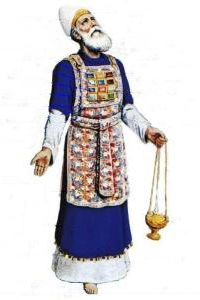
\includegraphics[width=50mm,scale=1.5]{Extras/Melchisedec.jpg}
\vspace{0.4in}  % Create a title for the document and write it in bold font
\LARGE{\textbf{\date}} % Again, do a line break
\linebreak 
% Create a subtitle \large{with Outlines, Statistics, Cross References, and Notes}
\vspace{0.5in}
\begin{flushleft}
\LARGE{Day \#55: Thursday, 24 February 2022  \\}\vspace{0.25in}
\LARGE{Deuteronomy 7-9 Psalm 55 Proverb 24}
\end{flushleft}
\vspace{0.6in}
\bigskip

\normalsize{Xenia, Oh.\\}
\normalsize{created: \today}
\vspace{1.3in}

\end{flushright}
\end{titlepage}

\newpage 
\tableofcontents\hypertarget{TOC}{}
\listoffigures
\listoftables

\hyphenation{A-bim-e-lech bre-thren E-phra-im  Gib-e-o-nites Jer-u-sa-lem through-out Phil-i-stines The-o-phil-us Am-a-le-kites ven-geance Mesh-el-e-mi-ah onan-ism Phar-a-oh thoughts grev-ous-ness Hach-a-liah adul-ter-er Shad-rach}

%%%%%%%%%%%%%%%%% EXTRA COLORS
%%%%%%%%%%%%%%%%% EXTRA COLORS
%%%%%%%%%%%%%%%%% EXTRA COLORS
\definecolor{champagne}{rgb}{0.97,0.91,0.81}
\definecolor{bone}{rgb}{0.89,0.85,0.79}

\definecolor{ForestGreen}{rgb}{0.00,0.29,0.098}
\definecolor{GIVING}{cmyk}{1,0.0,0.72,.1}

\definecolor{MLPE}{cmyk}{1,1,0,.45}
\definecolor{SOCCER}{cmyk}{.77, 0, .42, .49}
\definecolor{PAYBILL}{cmyk}{0,0.83,0.76,0.07}
\definecolor{SERMON}{cmyk}{.14,.9,0,.30} % aka seance \href{http://www.flatuicolorpicker.com/purple-cmyk-color-model/}{seance}
\definecolor{BIBLE}{cmyk}{0,.17,.74,.17}
\definecolor{WORKBLUE}{cmyk}{1, .5, 0, .6}
\definecolor{myOrange}{cmyk}{0, .4, .98, .03}
\definecolor{myTan}{cmyk}{0.0,.07,.17,.10}
\definecolor{myRed}{cmyk}{0,1,1,0}
\definecolor{myWhite}{cmyk}{0,0,0,0}
\definecolor{BLUESoD}{cmyk}{.97,.84,0,.04}
\definecolor{WHITE}{cmyk}{0,0,0,0}
\definecolor{OLDGOLD}{cmyk}{0.05,0.3,1.00,0}
\definecolor{CASTLETON}{cmyk}{1,0,0.31,0.66}
\definecolor{cadmiumgreen}{rgb}{0.0, 0.42, 0.24}
\definecolor{jungle}{rgb}{0.203,0.4882,0.1718}
\definecolor{MYGOLD}{rgb}{1,.84,0}

\definecolor{MYLIGHTGRAY}{rgb}{.85,.85,.85}

\definecolor{codegreen}{rgb}{0,0.6,0}
\definecolor{codegray}{rgb}{0.5,0.5,0.5}
\definecolor{codepurple}{rgb}{0.58,0,0.82}
\definecolor{backcolour}{rgb}{0.95,0.95,0.92}


\mdfdefinestyle{MyFrame}{%
    linecolor=blue,
    outerlinewidth=2pt,
    roundcorner=5pt,
    innertopmargin=\baselineskip,
    innerbottommargin=\baselineskip,
    innerrightmargin=10pt,
    innerleftmargin=10pt,
    backgroundcolor=gray!25!white}


\mdfdefinestyle{MyFrame2}{%
    linecolor=black,
    outerlinewidth=2pt,
    roundcorner=5pt,
    innertopmargin=\baselineskip,
    innerbottommargin=\baselineskip,
    innerrightmargin=10pt,
    innerleftmargin=10pt,
    backgroundcolor=yellow!25!white}


%%%%%
%% for PFTTIS list
%%%%%

%%% And Joseph said unto
\index[PFTTIS]{And Joseph said unto!Genesis!Gen 40:008}
\index[PFTTIS]{And Joseph said unto!Genesis!Gen 40:012}
\index[PFTTIS]{And Joseph said unto!Genesis!Gen 41:025}
\index[PFTTIS]{And Joseph said unto!Genesis!Gen 42:014}
\index[PFTTIS]{And Joseph said unto!Genesis!Gen 42:018}
\index[PFTTIS]{And Joseph said unto!Genesis!Gen 44:015}
\index[PFTTIS]{And Joseph said unto!Genesis!Gen 45:003}
\index[PFTTIS]{And Joseph said unto!Genesis!Gen 45:004}
\index[PFTTIS]{And Joseph said unto!Genesis!Gen 46:031}
\index[PFTTIS]{And Joseph said unto!Genesis!Gen 48:009}
\index[PFTTIS]{And Joseph said unto!Genesis!Gen 48:018}
\index[PFTTIS]{And Joseph said unto!Genesis!Gen 50:019}
\index[PFTTIS]{And Joseph said unto!Genesis!Gen 50:024}


%%% a shadow
\index[PFTTIS]{a shadow!1Chronicles!1Chr 029:15}
\index[PFTTIS]{a shadow!Job!Job 008:09}
\index[PFTTIS]{a shadow!Job!Job 014:02}
\index[PFTTIS]{a shadow!Job!Job 017:07}
\index[PFTTIS]{a shadow!Psalm!Psa 102:011}
\index[PFTTIS]{a shadow!Psalm!Psa 144:004}
\index[PFTTIS]{a shadow!Ecclesiastes!Eccl 006:012}
\index[PFTTIS]{a shadow!Ecclesiastes!Eccl 008:013}
\index[PFTTIS]{a shadow!Isaiah!Isa 04:006}
\index[PFTTIS]{a shadow!Isaiah!Isa 25:004}
\index[PFTTIS]{a shadow!Jonah!Jnh 04:06}
\index[PFTTIS]{a shadow!Colossians!Col 02:017}
\index[PFTTIS]{a shadow!Hebews!Heb 10:001}

%%% blessed is the man
\index[PFTTIS]{blessed is the man!Psalm!Psa 001:001}
\index[PFTTIS]{blessed is the man!Psalm!Psa 032:002}
\index[PFTTIS]{blessed is the man!Psalm!Psa 034:008}
\index[PFTTIS]{blessed is the man!Psalm!Psa 065:004}
\index[PFTTIS]{blessed is the man!Psalm!Psa 084:005}
\index[PFTTIS]{blessed is the man!Psalm!Psa 084:012}
\index[PFTTIS]{blessed is the man!Psalm!Psa 094:012}
\index[PFTTIS]{blessed is the man!Psalm!Psa 112:001}
\index[PFTTIS]{blessed is the man!Proverbs!Pro 008:034}
\index[PFTTIS]{blessed is the man!Isaiah!Isa 056:002}
\index[PFTTIS]{blessed is the man!Jeremiah!Jer 017:007}
\index[PFTTIS]{blessed is the man!Romans!Rom 004:008}
\index[PFTTIS]{blessed is the man!James!Jam 001:012}


%%% carry them
\index[PFTTIS]{carry them!Leviticus!Lev 14:045}
\index[PFTTIS]{carry them!Numbers!Num 11:012}
\index[PFTTIS]{carry them!Joshua!Jsh 04:003}
\index[PFTTIS]{carry them!1Samuel!1Sam 20:040}
\index[PFTTIS]{carry them!1Kings!1Kng 08:046}
\index[PFTTIS]{carry them!2Chronicles!2Chr 06:036}
\index[PFTTIS]{carry them!Ezra!Ezra 05:015}
\index[PFTTIS]{carry them!Isaiah!Isa 40:011}
\index[PFTTIS]{carry them!Isaiah!Isa 41:016}
\index[PFTTIS]{carry them!Isaiah!Isa 57:013}
\index[PFTTIS]{carry them!Jeremiah!Jer 20:004}
\index[PFTTIS]{carry them!Jeremiah!Jer 20:005}
\index[PFTTIS]{carry them!Jeremiah!Jer 43:012}


\index[PFTTIS]{good tidings!2Samuel!2Sam 18:027}
\index[PFTTIS]{good tidings!1Kings!1Ki 01:042}
\index[PFTTIS]{good tidings!2Kings!2Ki 07:009 (2x)}
\index[PFTTIS]{good tidings!Isaiah!Isa 40:009 (2x)}
\index[PFTTIS]{good tidings!Isaiah!Isa 41:007}
\index[PFTTIS]{good tidings!Isaiah!Isa 52:007}
\index[PFTTIS]{good tidings!Isaiah!Isa 61:001}
\index[PFTTIS]{good tidings!Nahum!Nah 01:005}
\index[PFTTIS]{good tidings!Luke!Lk 02:010}
\index[PFTTIS]{good tidings!1Thessalonians!1Thess 03:006}


%%% dead body
\index[PFTTIS]{dead body!Leviticus!Lev 21:011}
\index[PFTTIS]{dead body!Numbers!Num 06:006}
\index[PFTTIS]{dead body!Numbers!Num 09:006}
\index[PFTTIS]{dead body!Numbers!Num 09:007}
\index[PFTTIS]{dead body!Numbers!Num 09:010}
\index[PFTTIS]{dead body!Numbers!Num 09:011}
\index[PFTTIS]{dead body!Numbers!Num 09:013}
\index[PFTTIS]{dead body!Numbers!Num 09:016}
\index[PFTTIS]{dead body!2Kings!2Ki 08:005}
\index[PFTTIS]{dead body!Isaiah!Isa 26:019}
\index[PFTTIS]{dead body!Jeremiah!Jer 26:023}
\index[PFTTIS]{dead body!Jeremiah!Jer 36:030}
\index[PFTTIS]{dead body!Haggai!Hag 02:013}

%%% great sea
\index[PFTTIS]{great sea!Numbers!Num 34:006}
\index[PFTTIS]{great sea!Numbers!Num 34:007}
\index[PFTTIS]{great sea!Joshua!Jos 01:004}
\index[PFTTIS]{great sea!Joshua!Jos 09:001}
\index[PFTTIS]{great sea!Joshua!Jos 15:012}
\index[PFTTIS]{great sea!Joshua!Jos 15:047}
\index[PFTTIS]{great sea!Joshua!Jos 23:004}
\index[PFTTIS]{great sea!Ezekiel!Eze 47:010}
\index[PFTTIS]{great sea!Ezekiel!Eze 47:015}
\index[PFTTIS]{great sea!Ezekiel!Eze 47:019}
\index[PFTTIS]{great sea!Ezekiel!Eze 47:020}
\index[PFTTIS]{great sea!Ezekiel!Eze 48:028}
\index[PFTTIS]{great sea!Daniel!Dan 07:002}


%%% have forsaken me
\index[PFTTIS]{have forsaken me!Judges!Jdg 10:013}
\index[PFTTIS]{have forsaken me!1Samuel!1Sam 08:008}
\index[PFTTIS]{have forsaken me!1Kings!1Ki 11:033}
\index[PFTTIS]{have forsaken me!2Kings!2Ki 22:017}
\index[PFTTIS]{have forsaken me!2Chronicles!2Chr 12:005}
\index[PFTTIS]{have forsaken me!2Chronicles!2Chr 34:025}
\index[PFTTIS]{have forsaken me!Jeremiah!Jer 01:016}
\index[PFTTIS]{have forsaken me!Jeremiah!Jer 02:013}
\index[PFTTIS]{have forsaken me!Jeremiah!Jer 05:007}
\index[PFTTIS]{have forsaken me!Jeremiah!Jer 05:019}
\index[PFTTIS]{have forsaken me!Jeremiah!Jer 16:011 (2x)}
\index[PFTTIS]{have forsaken me!Jeremiah!Jer 19:004}

%%% no king
\index[PFTTIS]{no king!Judges!Jdg 17:06}
\index[PFTTIS]{no king!Judges!Jdg 18:01}
\index[PFTTIS]{no king!Judges!Jdg 19:01}
\index[PFTTIS]{no king!Judges!Jdg 21:25}
\index[PFTTIS]{no king!1Kings!1Ki 22:47}
\index[PFTTIS]{no king!2Kings!2Ki 23:25}
\index[PFTTIS]{no king!Nehemiah!Neh 13:26}
\index[PFTTIS]{no king!Psalms!Psa 033:016}
\index[PFTTIS]{no king!Proverbs!Pro 30:27}
\index[PFTTIS]{no king!Daniel!Dan 02:10}
\index[PFTTIS]{no king!Hosea!Hos 10:03}
\index[PFTTIS]{no king!Micah!Mic 04:09}
\index[PFTTIS]{no king!John!Jhn 19:15}


%%% rebellious house
\index[PFTTIS]{rebellious house!Exodus!Exo 02:005}
\index[PFTTIS]{rebellious house!Exodus!Exo 02:006}
\index[PFTTIS]{rebellious house!Exodus!Exo 02:008}
\index[PFTTIS]{rebellious house!Exodus!Exo 03:009}
\index[PFTTIS]{rebellious house!Exodus!Exo 03:026}
\index[PFTTIS]{rebellious house!Exodus!Exo 03:027}
\index[PFTTIS]{rebellious house!Exodus!Exo 12:002 (2x)}
\index[PFTTIS]{rebellious house!Exodus!Exo 12:003}
\index[PFTTIS]{rebellious house!Exodus!Exo 12:009}
\index[PFTTIS]{rebellious house!Exodus!Exo 12:025}
\index[PFTTIS]{rebellious house!Exodus!Exo 17:012}
\index[PFTTIS]{rebellious house!Exodus!Exo 24:003}

%%% seek him
\index[PFTTIS]{seek him!Deuteronomy!Deu 04:029}\index[PFTTIS]{seek him!1Samuel!1Sam 23:025}
\index[PFTTIS]{seek him!1Chronicles!1Chr 28:009}
\index[PFTTIS]{seek him!2Chronicles!1Chr 15:002}
\index[PFTTIS]{seek him!Ezra!Ezr 08:022}
\index[PFTTIS]{seek him!Psalms!Psa 022:026}
\index[PFTTIS]{seek him!Psalms!Psa 024:006}
\index[PFTTIS]{seek him!Psalms!Psa 119:002}
\index[PFTTIS]{seek him!SoS!SoS 03:002}
\index[PFTTIS]{seek him!SoS!SoS 06:001}
\index[PFTTIS]{seek him!Hosea!Hos 07:010}
\index[PFTTIS]{seek him!Amos!Amo 05:008}
\index[PFTTIS]{seek him!Hebrews!Heb 11:0063}


%%% seek ye
\index[PFTTIS]{seek ye!Isaiah!Isa 34:016}
\index[PFTTIS]{seek ye!Isaiah!Isa 45:019}
\index[PFTTIS]{seek ye!Isaiah!Isa 55:006}
\index[PFTTIS]{seek ye!Amos!Amos 5:004}
\index[PFTTIS]{seek ye!John!John 1:38}
\index[PFTTIS]{seek ye!John!John 18:4}
\index[PFTTIS]{seek ye!John!John 18:7}
\index[PFTTIS]{seek ye!Matthew!Matt 6:33}
\index[PFTTIS]{seek ye!Numbers!Num 16:10}
\index[PFTTIS]{seek ye!Luke!Luke 12:31}
\index[PFTTIS]{seek ye!Luke!Luke 24:5}
\index[PFTTIS]{seek ye!Psalm!Psa 27:8}
\index[PFTTIS]{seek ye!Zephaniah!Zeph 2:3}

%%% the uncircumcised
\index[PFTTIS]{the uncircumcised!Genesis!Gen 17:014}
\index[PFTTIS]{the uncircumcised!Judges!Jdg 14:003}
\index[PFTTIS]{the uncircumcised!Judges!Jdg 15:018}
\index[PFTTIS]{the uncircumcised!2Samuel!2Sam 01:020}
\index[PFTTIS]{the uncircumcised!Isaiah!Isa 02:001}
\index[PFTTIS]{the uncircumcised!Jeremiah!Jer 09:025}
\index[PFTTIS]{the uncircumcised!Ezekiel!Eze 28:010}
\index[PFTTIS]{the uncircumcised!Ezekiel!Eze 31:018}
\index[PFTTIS]{the uncircumcised!Ezekiel!Eze 32:019}
\index[PFTTIS]{the uncircumcised!Ezekiel!Eze 32:027}
\index[PFTTIS]{the uncircumcised!Ezekiel!Eze 32:028}
\index[PFTTIS]{the uncircumcised!Ezekiel!Eze 32:029}
\index[PFTTIS]{the uncircumcised!Ezekiel!Eze 32:032}

%%% worship him
\index[PFTTIS]{worship him!Psalms!Psa 97:007}
\index[PFTTIS]{worship him!Zephaniah!Zeph 02:011}
\index[PFTTIS]{worship him!Matthew!Matt 02:002}
\index[PFTTIS]{worship him!Matthew!Matt 02:008}
\index[PFTTIS]{worship him!John!John 04:023}
\index[PFTTIS]{worship him!John!John 04:024 (2x)} 
\index[PFTTIS]{worship him!Acts!Acts 17:023}
\index[PFTTIS]{worship him!Hebrews!Heb 01:006}
\index[PFTTIS]{worship him!Revelation!Rev 04:010}
\index[PFTTIS]{worship him!Revelation!Rev 13:008}
\index[PFTTIS]{worship him!Revelation!Rev 14:007}
\index[PFTTIS]{worship him!Revelation!Rev 19:010}


%%%%%
%% for PFTTIS list
%%%%%

%%% afflictions
\index[WFTTIS]{afflictions!Psalms!Psa 34:019}
\index[WFTTIS]{afflictions!Psalms!Psa 132:001}
\index[WFTTIS]{afflictions!Acts!Acts 07:010}
\index[WFTTIS]{afflictions!Acts!Acts 20:023}
\index[WFTTIS]{afflictions!2Corinthians!2Cor 06:004}
\index[WFTTIS]{afflictions!Colossians!Col 01:024}
\index[WFTTIS]{afflictions!1Thessalonians!1Thess 03:003}
\index[WFTTIS]{afflictions!2Timothy!2Tim 01:008}
\index[WFTTIS]{afflictions!2Timothy!2Tim 03:011}
\index[WFTTIS]{afflictions!2Timothy!2Tim 04:005}
\index[WFTTIS]{afflictions!Hebrews!Heb 10:032}
\index[WFTTIS]{afflictions!Hebrews!Heb 10:033}
\index[WFTTIS]{afflictions!1Peter!1Pet 05:009}

%%% acsend
\index[WFTTIS]{acsend!Joshua!Jos 06:05}
\index[WFTTIS]{acsend!Psalm!Psa 024:003}
\index[WFTTIS]{acsend!Psalm!Psa 135:007}
\index[WFTTIS]{acsend!Psalm!Psa 139:008}
\index[WFTTIS]{acsend!Isaiah!Isa 14:013}
\index[WFTTIS]{acsend!Isaiah!Isa 14:014}
\index[WFTTIS]{acsend!Jeremiah!Jer 10:013}
\index[WFTTIS]{acsend!Jeremiah!Jer 51:016}
\index[WFTTIS]{acsend!Ezekiel!Eze 38:009}
\index[WFTTIS]{acsend!John!John 06:062}
\index[WFTTIS]{acsend!John!John 20:017}
\index[WFTTIS]{acsend!Romans!Rom 10:006}
\index[WFTTIS]{acsend!Revelation!Rev 17:008}

%%% Assyrian
\index[WFTTIS]{Assyrian!Isaiah!Isa 10:005}
\index[WFTTIS]{Assyrian!Isaiah!Isa 10:024}
\index[WFTTIS]{Assyrian!Isaiah!Isa 14:025}
\index[WFTTIS]{Assyrian!Isaiah!Isa 19:023}
\index[WFTTIS]{Assyrian!Isaiah!Isa 23:013}
\index[WFTTIS]{Assyrian!Isaiah!Isa 30:031}
\index[WFTTIS]{Assyrian!Isaiah!Isa 31:008}
\index[WFTTIS]{Assyrian!Isaiah!Isa 52:004}
\index[WFTTIS]{Assyrian!Ezekiel!Eze 31:003}
\index[WFTTIS]{Assyrian!Hosea!Hos 05:013}
\index[WFTTIS]{Assyrian!Hosea!Hos 11:005}
\index[WFTTIS]{Assyrian!Micah!Hos 05:005}
\index[WFTTIS]{Assyrian!Micah!Hos 05:006}

%%% blot
\index[WFTTIS]{blot!Exodus!Exo 32:032}
\index[WFTTIS]{blot!Exodus!Exo 32:033}
\index[WFTTIS]{blot!Numbers!Num 05:026}
\index[WFTTIS]{blot!Deuteronomy!Deut 09:014}
\index[WFTTIS]{blot!Deuteronomy!Deut 25:019}
\index[WFTTIS]{blot!Deuteronomy!Deut 29:020}
\index[WFTTIS]{blot!2Kings!2Ki 14:027}
\index[WFTTIS]{blot!Job!Job 31:007}
\index[WFTTIS]{blot!Psalms!Psa 51:001}
\index[WFTTIS]{blot!Psalms!Psa 51:009}
\index[WFTTIS]{blot!Proverbs!Pro 09:007}
\index[WFTTIS]{blot!Jeremiah!Jer 18:023}
\index[WFTTIS]{blot!Revelation!Rev 03:005}


%%% chain
\index[WFTTIS]{chain!Genesis!Gen 41:042}
\index[WFTTIS]{chain!1Kings!1Ki 07:017}
\index[WFTTIS]{chain!Psalms!Psa 73:006}
\index[WFTTIS]{chain!SoS!Sos 04:009}
\index[WFTTIS]{chain!Lamentations!Lam 03:007}
\index[WFTTIS]{chain!Ezekiel!Eze 07:023}
\index[WFTTIS]{chain!Ezekiel!Eze 16:011}
\index[WFTTIS]{chain!Daniel!Dan 05:007}
\index[WFTTIS]{chain!Daniel!Dan 05:016}
\index[WFTTIS]{chain!Daniel!Dan 05:029}
\index[WFTTIS]{chain!Acts!Acts 28:020}
\index[WFTTIS]{chain!2Timothy!2Tim 01:016}
\index[WFTTIS]{chain!Revelation!Rev 20:001}


%%% controversy
\index[WFTTIS]{controversy!Deuteronomy!Deu 17:008}
\index[WFTTIS]{controversy!Deuteronomy!Deu 19:017}
\index[WFTTIS]{controversy!Deuteronomy!Deu 21:005}
\index[WFTTIS]{controversy!Deuteronomy!Deu 25:001}
\index[WFTTIS]{controversy!2Samuel!2Sam 15:002}
\index[WFTTIS]{controversy!Isaiah!Isa 34:008}
\index[WFTTIS]{controversy!Jeremiah!Jer 25:031}
\index[WFTTIS]{controversy!Ezekiel!Eze 44:024}
\index[WFTTIS]{controversy!Hosea!Hos 04:001}
\index[WFTTIS]{controversy!Hosea!Hos 12:002}
\index[WFTTIS]{controversy!Micah!Mic 06:002 (2x)}
\index[WFTTIS]{controversy!1Timothy!1Tim 03:016}


%%% Dagon/Dagon's
\index[WFTTIS]{Dagon!Judges!Jdg 16:023}
\index[WFTTIS]{Dagon!1Samuel!1Sam 05:002 (2x)}
\index[WFTTIS]{Dagon!1Samuel!1Sam 05:003 (2x)}
\index[WFTTIS]{Dagon!1Samuel!1Sam 05:004 (3x)}
\index[WFTTIS]{Dagon!1Samuel!1Sam 05:005 (3x)}
\index[WFTTIS]{Dagon!1Samuel!1Sam 05:007}
\index[WFTTIS]{Dagon!1Chronicles!1Chr 10:010}

%%% disobedient
\index[WFTTIS]{disobedient!1Kings!1Ki 13:026}
\index[WFTTIS]{disobedient!Nehemiah!Neh 09:026}
\index[WFTTIS]{disobedient!Luke!Luke 01:017}
\index[WFTTIS]{disobedient!Acts!Acts 26:019}
\index[WFTTIS]{disobedient!Romans!Rom 01:030}
\index[WFTTIS]{disobedient!Romans!Rom 10:021}
\index[WFTTIS]{disobedient!1Timothy!1Tim 01:009}
\index[WFTTIS]{disobedient!2Timothy!2Tim 03:002}
\index[WFTTIS]{disobedient!Titus!Titus 01:016}
\index[WFTTIS]{disobedient!Titus!Titus 03:003}
\index[WFTTIS]{disobedient!1Peter!1Pet 02:007}
\index[WFTTIS]{disobedient!1Peter!1Pet 02:008}
\index[WFTTIS]{disobedient!1Peter!1Pet 03:020}


%%% doubt
\index[WFTTIS]{doubt!Genesis!Gen 37:033}
\index[WFTTIS]{doubt!Deuteronomy!Deu 28:066}
\index[WFTTIS]{doubt!Job!Job 12:002}
\index[WFTTIS]{doubt!Matthew!Matt 14:031}
\index[WFTTIS]{doubt!Matthew!Matt 21:021}
\index[WFTTIS]{doubt!Mark!Mk 11:023}
\index[WFTTIS]{doubt!Luke!Lk 11:020}
\index[WFTTIS]{doubt!John!Jhn 10:024}
\index[WFTTIS]{doubt!Acts!Acts 02:012}
\index[WFTTIS]{doubt!Acts!Acts 28:004}
\index[WFTTIS]{doubt!1Corinthians!1Cor 09:010}
\index[WFTTIS]{doubt!Galatians!Gal 04:020}
\index[WFTTIS]{doubt!1John!1Jhn 02:019}


%%% dungeon
\index[WFTTIS]{dungeon!Genesis!Gen 40:015}
\index[WFTTIS]{dungeon!Genesis!Gen 41:014}
\index[WFTTIS]{dungeon!Exodus!Exo 12:029}
\index[WFTTIS]{dungeon!Jeremiah!Jer 37:016}
\index[WFTTIS]{dungeon!Jeremiah!Jer 38:006 (2x)}
\index[WFTTIS]{dungeon!Jeremiah!Jer 38:007}
\index[WFTTIS]{dungeon!Jeremiah!Jer 38:009}
\index[WFTTIS]{dungeon!Jeremiah!Jer 38:010}
\index[WFTTIS]{dungeon!Jeremiah!Jer 38:011}
\index[WFTTIS]{dungeon!Jeremiah!Jer 38:013}
\index[WFTTIS]{dungeon!Lamentations!Lam 03:053}
\index[WFTTIS]{dungeon!Lamentations!Lam 03:055}


%%% error
\index[WFTTIS]{error!2Samuel!2Sam 06:007}
\index[WFTTIS]{error!Job!Job 19:004}
\index[WFTTIS]{error!Ecclesiastes!Ecc 05:006}
\index[WFTTIS]{error!Ecclesiastes!Ecc 10:005}
\index[WFTTIS]{error!Isaiah!Isa 32:006}
\index[WFTTIS]{error!Daniel!Dan 06:004}
\index[WFTTIS]{error!Matthew!Matt 27:064}
\index[WFTTIS]{error!Romans!Rom 01:027}
\index[WFTTIS]{error!James!Jam 05:020}
\index[WFTTIS]{error!2Peter!2Pet 02:018}
\index[WFTTIS]{error!2Peter!2Pet 03:017}
\index[WFTTIS]{error!1John!1Jn 04:006}
\index[WFTTIS]{error!Jude!Jude 01:011}

%%% fourish
\index[WFTTIS]{fourish!Psalms!Psa 072:007}
\index[WFTTIS]{fourish!Psalms!Psa 072:016}
\index[WFTTIS]{fourish!Psalms!Psa 092:007}
\index[WFTTIS]{fourish!Psalms!Psa 092:012}
\index[WFTTIS]{fourish!Psalms!Psa 092:013}
\index[WFTTIS]{fourish!Psalms!Psa 132:018}
\index[WFTTIS]{fourish!Proverbs!Pro 11:28}
\index[WFTTIS]{fourish!Proverbs!Pro 14:11}
\index[WFTTIS]{fourish!Ecclesiastes!Ecc 12:05}
\index[WFTTIS]{fourish!SongOfSolomon!SOS 07:12}
\index[WFTTIS]{fourish!Isaiah!Isa 17:11}
\index[WFTTIS]{fourish!Isaiah!Isa 66:14}
\index[WFTTIS]{fourish!Ezekiel!Eze 17:24}




%%% giants
\index[WFTTIS]{giants!Genesis!Gen 06:004}
\index[WFTTIS]{giants!Numbers!Num 13:033}
\index[WFTTIS]{giants!Deuteronomy!Deut 02:011}
\index[WFTTIS]{giants!Deuteronomy!Deut 02:021}
\index[WFTTIS]{giants!Deuteronomy!Deut 03:011}
\index[WFTTIS]{giants!Deuteronomy!Deut 03:013}
\index[WFTTIS]{giants!Joshua!Josh 12:004}
\index[WFTTIS]{giants!Joshua!Josh 13:012}
\index[WFTTIS]{giants!Joshua!Josh 15:008}
\index[WFTTIS]{giants!Joshua!Josh 17:015}
\index[WFTTIS]{giants!Joshua!Josh 16:016}

%%% good man
\index[WFTTIS]{good man!2 Samuel!2Sa 18:27}
%(1) Psalms 37:23 [5]
%(1) Psalms 112:5 [2]
%(1) Proverbs 12:2 [2]
%(1) Proverbs 13:22 [2]
%(1) Proverbs 14:14 [14]
%(1) Micah 7:2 [2]
%(1) Matthew 12:35 [2]
%(1) Luke 6:45 [2]
%(1) Luke 23:50 [15]
%(1) John 7:12 [17]
%(1) Acts 11:24 [5]
%(1) Romans 5:7 [14]

%%% Hinnom
\index[WFTTIS]{Hinnom!Joshua!Jsh 15:008}
\index[WFTTIS]{Hinnom!Joshua!Jsh 18:016}
\index[WFTTIS]{Hinnom!2Kings!2Ki 23:010}
\index[WFTTIS]{Hinnom!2Chronicles!2Chr 28:003}
\index[WFTTIS]{Hinnom!2Chronicles!2Chr 33:006}
\index[WFTTIS]{Hinnom!Nehemiah!Neh 11:030}
\index[WFTTIS]{Hinnom!Jeremiah!Jer 07:031}
\index[WFTTIS]{Hinnom!Jeremiah!Jer 07:032}
\index[WFTTIS]{Hinnom!Jeremiah!Jer 19:002}
\index[WFTTIS]{Hinnom!Jeremiah!Jer 19:006}
\index[WFTTIS]{Hinnom!Jeremiah!Jer 32:035}

%%% inclined
\index[WFTTIS]{inclined!Judges!Jdg 09:003}
\index[WFTTIS]{inclined!Psalms!Psa 040:001}
\index[WFTTIS]{inclined!Psalms!Psa 116:002}
\index[WFTTIS]{inclined!Psalms!Psa 119:112}
\index[WFTTIS]{inclined!Proverbs!Pro 05:13}
\index[WFTTIS]{inclined!Jeremiah!Jer 07:24}
\index[WFTTIS]{inclined!Jeremiah!Jer 07:26}
\index[WFTTIS]{inclined!Jeremiah!Jer 11:08}
\index[WFTTIS]{inclined!Jeremiah!Jer 17:23}
\index[WFTTIS]{inclined!Jeremiah!Jer 25:04}
\index[WFTTIS]{inclined!Jeremiah!Jer 34:14}
\index[WFTTIS]{inclined!Jeremiah!Jer 35:15}
\index[WFTTIS]{inclined!Jeremiah!Jer 44:05}


%%% laughed
\index[WFTTIS]{laughed!Genesis!Gen 17:017}
\index[WFTTIS]{laughed!Genesis!Gen 18:012}
\index[WFTTIS]{laughed!Genesis!Gen 18:015}
\index[WFTTIS]{laughed!2Kings!2Ki 19:021}
\index[WFTTIS]{laughed!2Chronicles!2Chr 30:010}
\index[WFTTIS]{laughed!Nehemiah!Neh 02:019}
\index[WFTTIS]{laughed!Job!Job 12:004}
\index[WFTTIS]{laughed!Job!Job 29:024}
\index[WFTTIS]{laughed!Isaiah!Isa 37:022}
\index[WFTTIS]{laughed!Ezekiel!Ezek 23:032}
\index[WFTTIS]{laughed!Matthew!Matt 09:024}
\index[WFTTIS]{laughed!Mark!Mk 05:040}
\index[WFTTIS]{laughed!Luke!Lk 08:053}

%%% liar
\index[WFTTIS]{liar!Job!Job 24:025}
\index[WFTTIS]{liar!Proverbs!Pro 17:004}
\index[WFTTIS]{liar!Proverbs!Pro 19:022}
\index[WFTTIS]{liar!Proverbs!Pro 30:006}
\index[WFTTIS]{liar!Jeremiah!Jer 15:018}
\index[WFTTIS]{liar!John!Jhn 08:044}
\index[WFTTIS]{liar!John!Jhn 08:055}
\index[WFTTIS]{liar!Romans!Rom 03:004}
\index[WFTTIS]{liar!1John!1Jhn 01:010}
\index[WFTTIS]{liar!1John!1Jhn 02:004}
\index[WFTTIS]{liar!1John!1Jhn 02:022}
\index[WFTTIS]{liar!1John!1Jhn 04:020}
\index[WFTTIS]{liar!1John!1Jhn 05:010}

%%% palsy
\index[WFTTIS]{palsy!Matthew!Matt 04:024}
\index[WFTTIS]{palsy!Matthew!Matt 08:006}
\index[WFTTIS]{palsy!Matthew!Matt 09:002}
\index[WFTTIS]{palsy!Matthew!Matt 09:006}
\index[WFTTIS]{palsy!Mark!Mk 02:003}
\index[WFTTIS]{palsy!Mark!Mk 02:004}
\index[WFTTIS]{palsy!Mark!Mk 02:005}
\index[WFTTIS]{palsy!Mark!Mk 02:009}
\index[WFTTIS]{palsy!Mark!Mk 02:010}
\index[WFTTIS]{palsy!Luke!Lk 05:018}
\index[WFTTIS]{palsy!Luke!Lk 05:024}
\index[WFTTIS]{palsy!Acts!Acts 09:033}

%%% Profitable
\index[WFTTIS]{profitable!Job!Job 22:002 (2x)}
\index[WFTTIS]{profitable!Ecclesiastes!Ecc 10:010}
\index[WFTTIS]{profitable!Isaiah!Isa 44:010}
\index[WFTTIS]{profitable!Jeremiah!Jer 13:007}
\index[WFTTIS]{profitable!Matthew!Matt 05:029}
\index[WFTTIS]{profitable!Matthew!Matt 05:030}
\index[WFTTIS]{profitable!Acts!Acts 20:020}
\index[WFTTIS]{profitable!1Timothy!1Tim 04:008}
\index[WFTTIS]{profitable!2Timothy!2Tim 03:016}
\index[WFTTIS]{profitable!2Timothy!2Tim 04:011}
\index[WFTTIS]{profitable!Titus!Titus 03:008}
\index[WFTTIS]{profitable!Philemon!Phlm 01:011}

%%% Rechab
\index[WFTTIS]{Rechab!2Samuel!2Sam 04:002}
\index[WFTTIS]{Rechab!2Samuel!2Sam 04:005}
\index[WFTTIS]{Rechab!2Samuel!2Sam 04:006}
\index[WFTTIS]{Rechab!2Samuel!2Sam 04:009}
\index[WFTTIS]{Rechab!2KIngs!2Ki 10:015}
\index[WFTTIS]{Rechab!2KIngs!2Ki 10:023}
\index[WFTTIS]{Rechab!1Chronicles!1Chr 02:055}
\index[WFTTIS]{Rechab!Nehemiah!Neh 03:014}
\index[WFTTIS]{Rechab!Jeremiah!Jer 35:006}
\index[WFTTIS]{Rechab!Jeremiah!Jer 35:008}
\index[WFTTIS]{Rechab!Jeremiah!Jer 35:014}
\index[WFTTIS]{Rechab!Jeremiah!Jer 35:016}
\index[WFTTIS]{Rechab!Jeremiah!Jer 35:019}

%%% serpents
\index[WFTTIS]{serpents!Exodus!Exo 07:012}
\index[WFTTIS]{serpents!Numbers!Num 21:006}
\index[WFTTIS]{serpents!Numbers!Num 21:007}
\index[WFTTIS]{serpents!Deuteronomy!Deu 08:015}
\index[WFTTIS]{serpents!Deuteronomy!Deu 32:024}
\index[WFTTIS]{serpents!Jeremiah!Jer 08:017}
\index[WFTTIS]{serpents!Matthew!Matt 10:016}
\index[WFTTIS]{serpents!Matthew!Matt 23:033}
\index[WFTTIS]{serpents!Mark!Mk 16:018}
\index[WFTTIS]{serpents!Luke!Lk 10:019}
\index[WFTTIS]{serpents!1Corinthians!1Cor 10:009}
\index[WFTTIS]{serpents!James!Jas 03:007}
\index[WFTTIS]{serpents!Revelation!Rev 09:019}

%%% short
\index[WFTTIS]{short!Numbers!Num 11:023}
\index[WFTTIS]{short!2Kings!2Ki 10:032}
\index[WFTTIS]{short!Job!Job 17:012}
\index[WFTTIS]{short!Job!Job 20:005}
\index[WFTTIS]{short!Psalms!Psa 89:047}
\index[WFTTIS]{short!Romans!Rom 03:023}
\index[WFTTIS]{short!Romans!Rom 09:028  (2x)}
\index[WFTTIS]{short!1Corinthians!1Cor 07:029}
\index[WFTTIS]{short!1Thessalonians!1Thess 02:017}
\index[WFTTIS]{short!Hebrews!Heb 04:001}
\index[WFTTIS]{short!Revelation!Rev 12:012}
\index[WFTTIS]{short!Revelation!Rev 17:010}

%%% smiteth
\index[WFTTIS]{smiteth!Exodus!Exo 21:012}
\index[WFTTIS]{smiteth!Exodus!Exo 21:15}
\index[WFTTIS]{smiteth!Deuteronomy!Dt 25:11}
\index[WFTTIS]{smiteth!Deuteronomy!Dt 27:24}
\index[WFTTIS]{smiteth!Joshua!Jsh 15:16}
\index[WFTTIS]{smiteth!Judges!Jdg 15:16}
\index[WFTTIS]{smiteth!2 Samuel!2Sa 05:08}
\index[WFTTIS]{smiteth!1Chronicles!1Chr 11:06}
\index[WFTTIS]{smiteth!Job!1Chr 26:12}
\index[WFTTIS]{smiteth!Isaiah!Isa 09:13}
\index[WFTTIS]{smiteth!Lamentations!Lam 03:30}
\index[WFTTIS]{smiteth!Ezekiel!Eze 07:09}
\index[WFTTIS]{smiteth!Luke!Lk 06:29}



%%% vanities
\index[WFTTIS]{vanities!Deuteronomy!Deut 21:021}
\index[WFTTIS]{vanities!1Kings!1Ki 16:013}
\index[WFTTIS]{vanities!1Kings!1Ki 16:026}
\index[WFTTIS]{vanities!Psalms!Psa 031:006}
\index[WFTTIS]{vanities!Ecclesiastes!Ecc 01:002 (2x)}
\index[WFTTIS]{vanities!Ecclesiastes!Ecc 05:007}
\index[WFTTIS]{vanities!Ecclesiastes!Ecc 12:008}
\index[WFTTIS]{vanities!Jeremiah!Jer 08:019}
\index[WFTTIS]{vanities!Jeremiah!Jer 10:008}
\index[WFTTIS]{vanities!Jeremiah!Jer 14:022}
\index[WFTTIS]{vanities!Jonah!Jnh 02:008}
\index[WFTTIS]{vanities!Acts!Acts 14:015}



%%%%%
%% for PFTTIS list
%%%%%

%%% worm
\index[WFITV]{worm!Exodus!Exo 16:024}
\index[WFITV]{worm!Job!Job 17:014}
\index[WFITV]{worm!Job!Job 24:029}
\index[WFITV]{worm!Job!Job 25:005 (2x)}
\index[WFITV]{worm!Psalms!Psa 022:006}
\index[WFITV]{worm!Isaiah!Isa 14:011}
\index[WFITV]{worm!Isaiah!Isa 41:014}
\index[WFITV]{worm!Isaiah!Isa 51:008}
\index[WFITV]{worm!Isaiah!Isa 66:024}
\index[WFITV]{worm!Jonah!Jnh 04:007}
\index[WFITV]{worm!Mark!Mk 09:044}
\index[WFITV]{worm!Mark!Mk 09:046}
\index[WFITV]{worm!Mark!Mk 09:048}


%\subsubsection{Title}
%\textbf{Introduction:} Isaiah 46 
%\index[speaker]{Speaker!Isaiah 49 (Title}
%\index[series]{Book (Speaker)!IPassage (Title)}
%\index[date]{2017/07/09!Isaiah 49 (Title)}
%\begin{compactenum}[I.]
%    \item  \textbf{Point} \index[scripture]{Isaiah!IPassage} (IPassage)
%\end{compactenum}




  


%\input{02OT-Exodus/ExodusIntroduction}

%\newpage
%\begin{figure}
%\begin{center}
%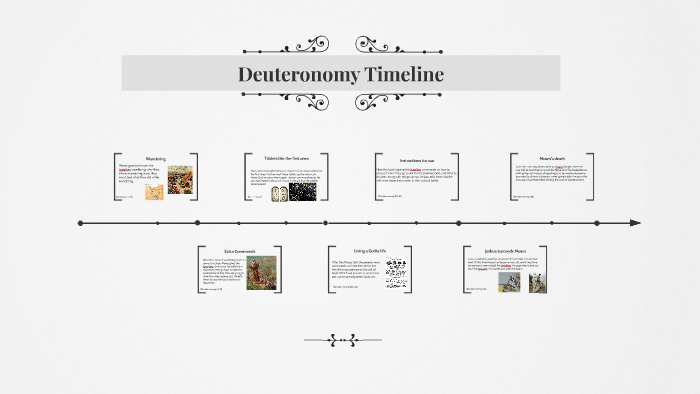
\includegraphics[scale=.7, angle=0]{05OT-Deuteronomy/References/AndrewSmithDeuteronomyTimeline.png}
%\caption[Deuteronomy Timeline by Andrew Smith]{Deuteronomy Timeline by Andrew %Smith}
%\label{fig:Deuteronomy Timeline by Andrew Smith}
%\end{center}
%\end{figure}

\newpage
\begin{figure}
\begin{center}
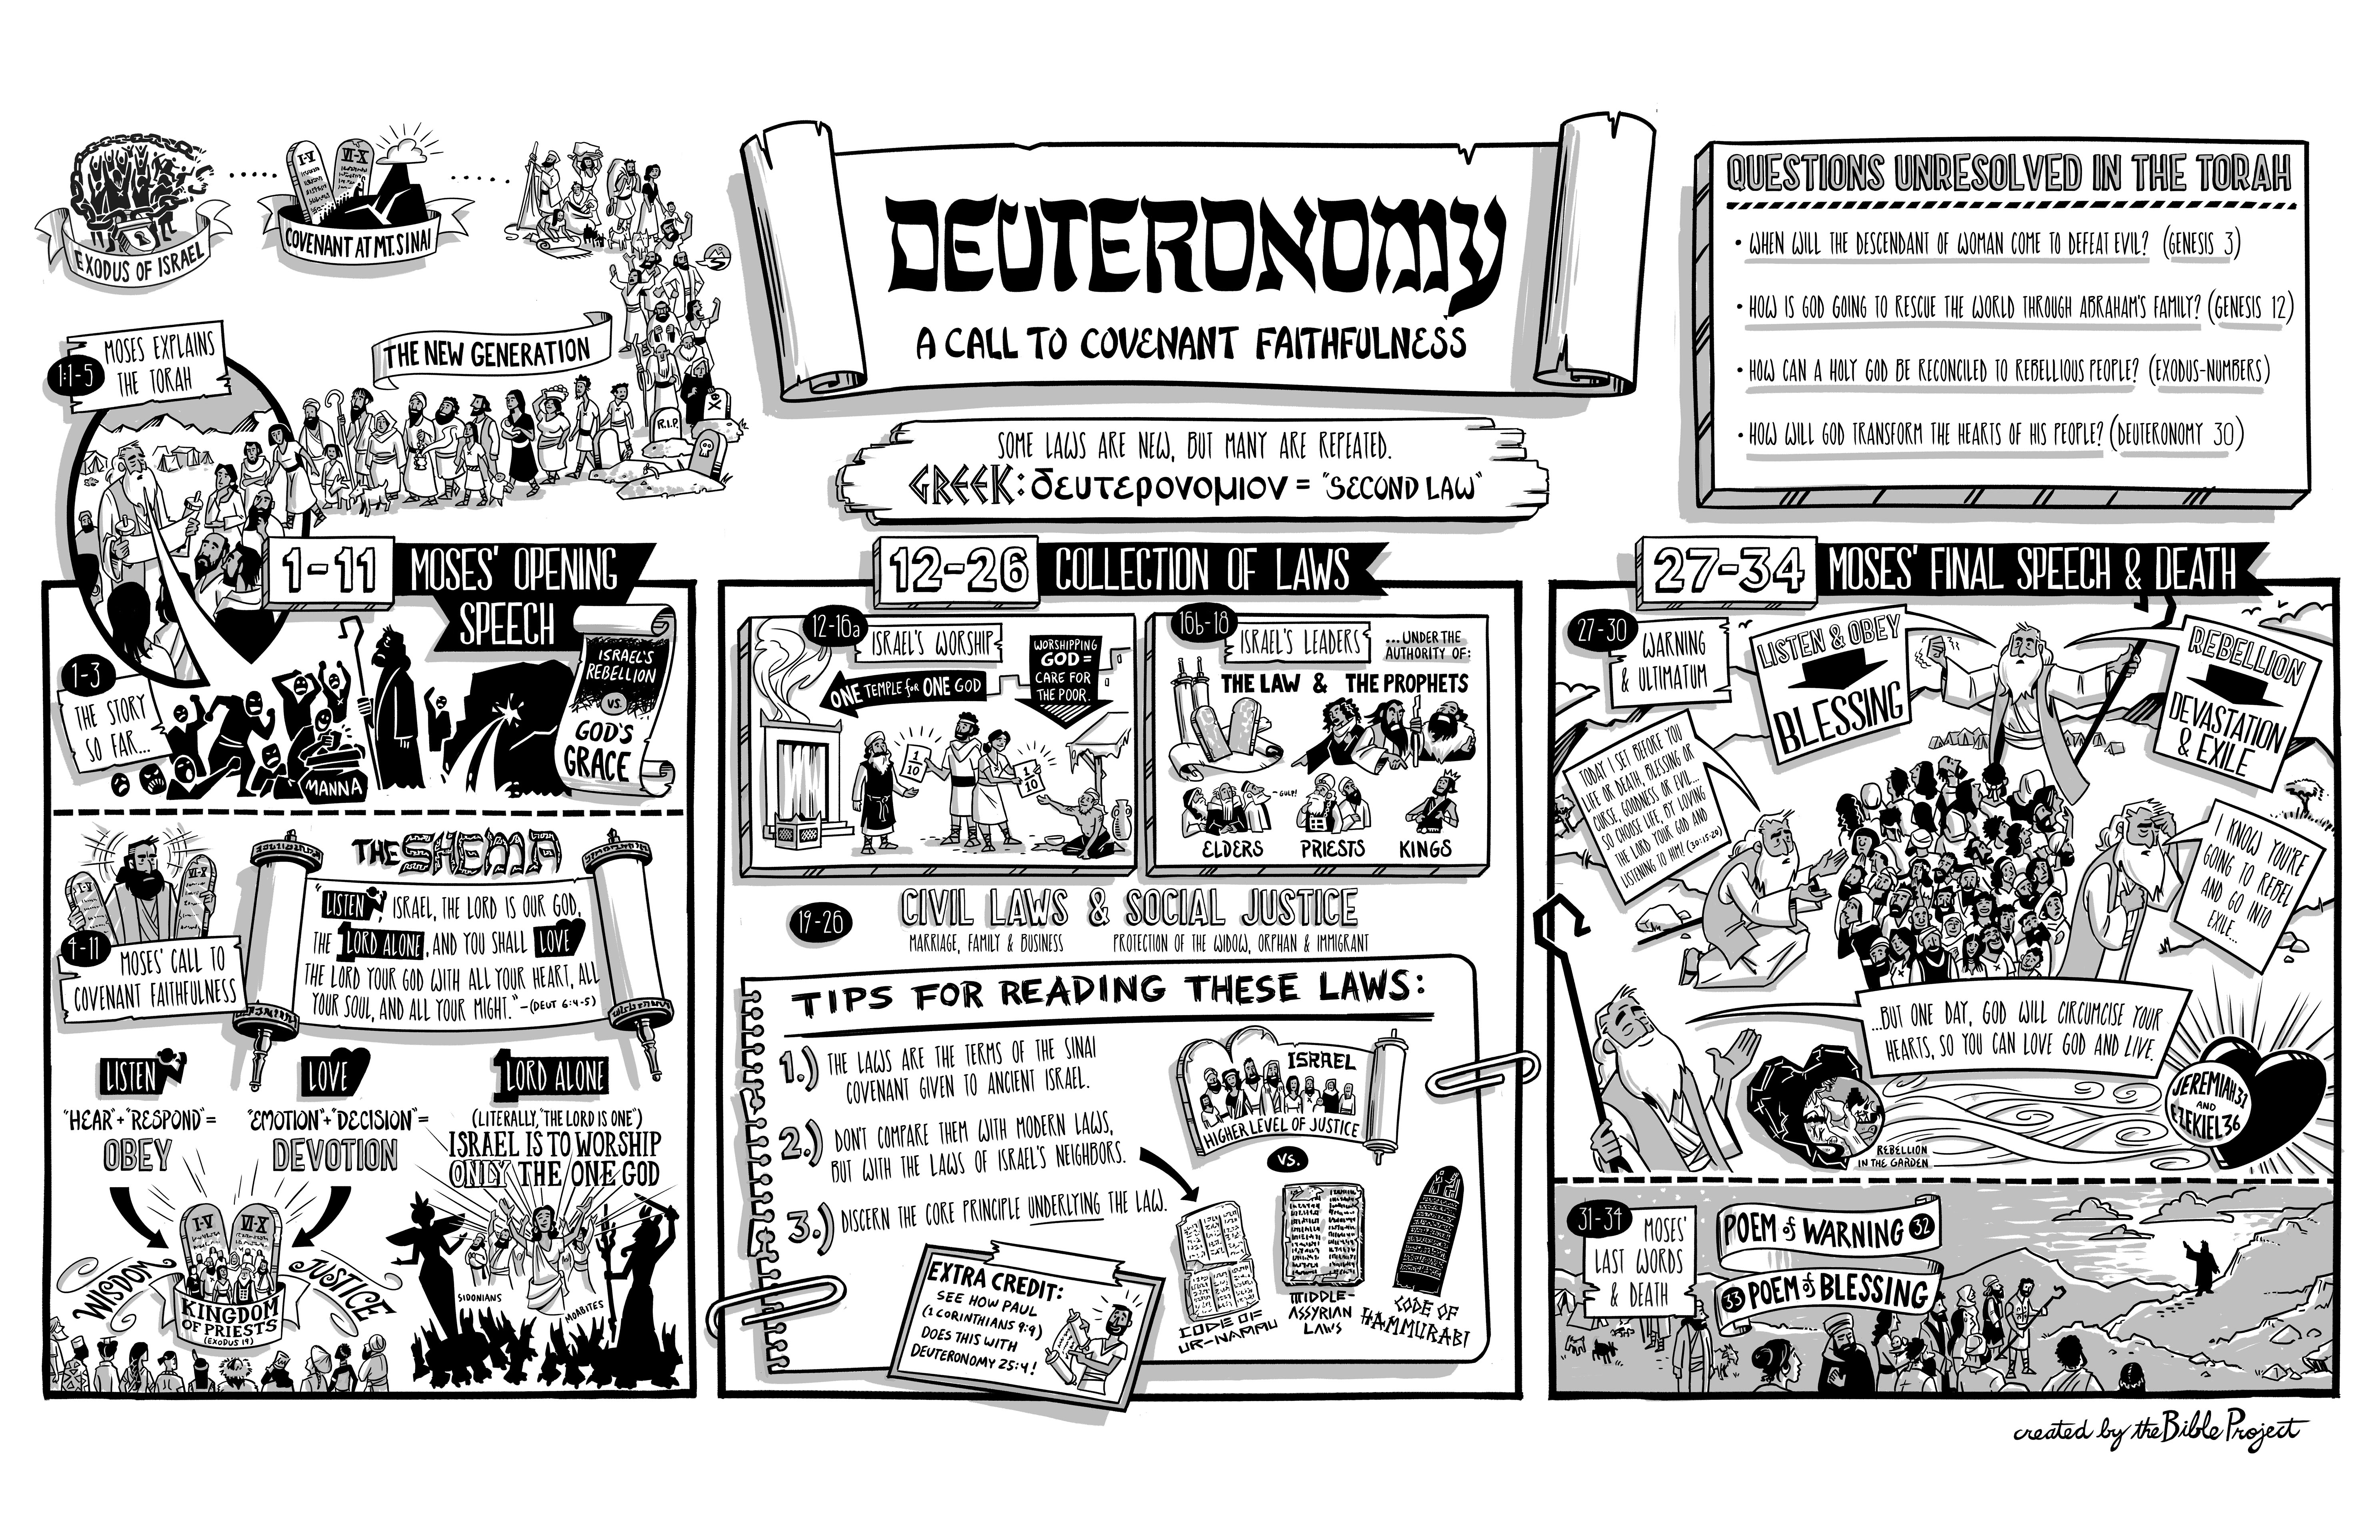
\includegraphics[scale=0.5, angle=90]{05OT-Deuteronomy/References/BibleProject-Deuteronomy.jpg}
\caption[Deuteronomy from the Bible Project]{Deuteronomy from the Bible Project}
\label{fig:Deuteronomy from the Bible Project}
\end{center}
\end{figure}

\newpage
\begin{figure}
\begin{center}
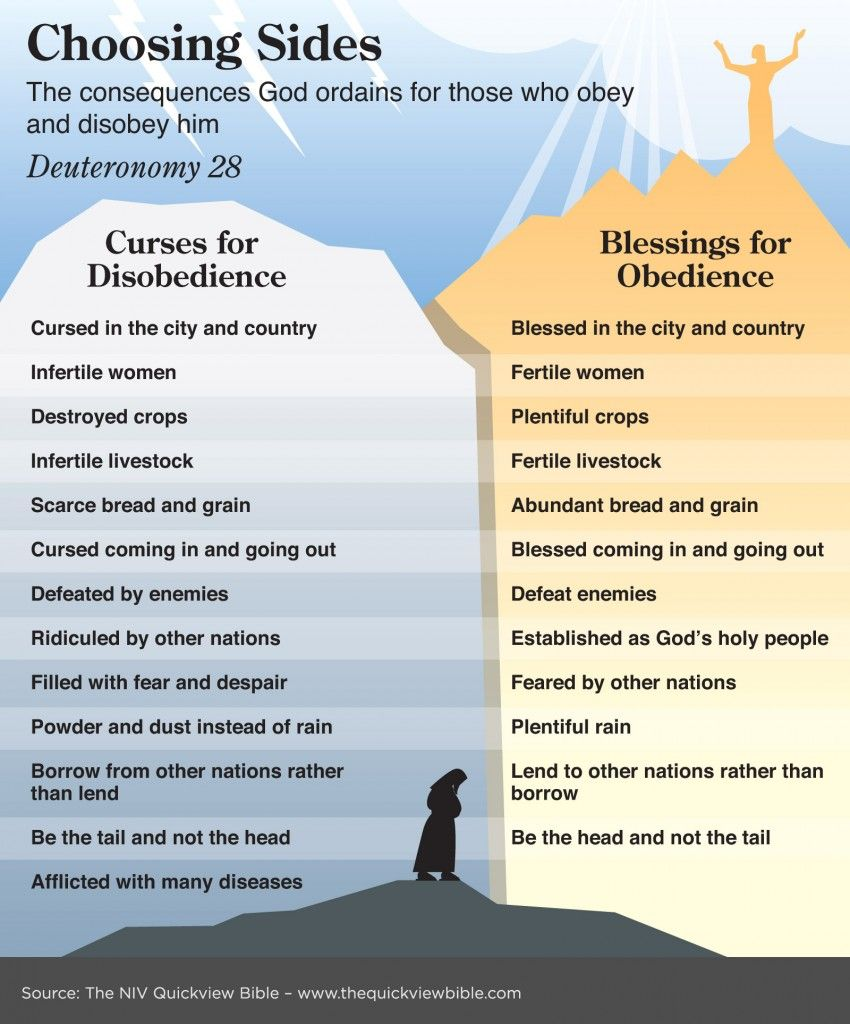
\includegraphics[scale=0.5, angle=0]{05OT-Deuteronomy/References/ChoosingSides.jpeg}
\caption[Choosing Sides]{Choosing Sides}
\label{fig:Choosing Sides}
\end{center}
\end{figure}

\newpage
\begin{figure}
\begin{center}
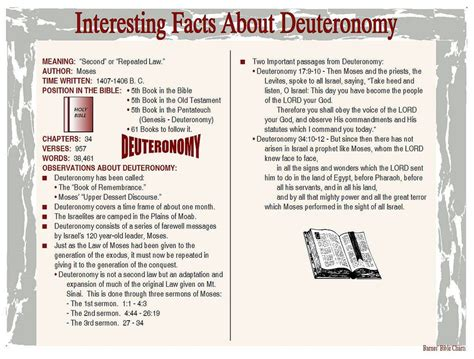
\includegraphics[scale=0.8, angle=90]{05OT-Deuteronomy/References/interestingfactsaboutdeuteronomy.jpeg}
\caption[Interesting Facts About Deuteronomy]{Interesting Facts About Deuteronomy}
\label{fig:Interesting Facts About Deuteronomy}
\end{center}
\end{figure}

\newpage
\begin{figure}
\begin{center}
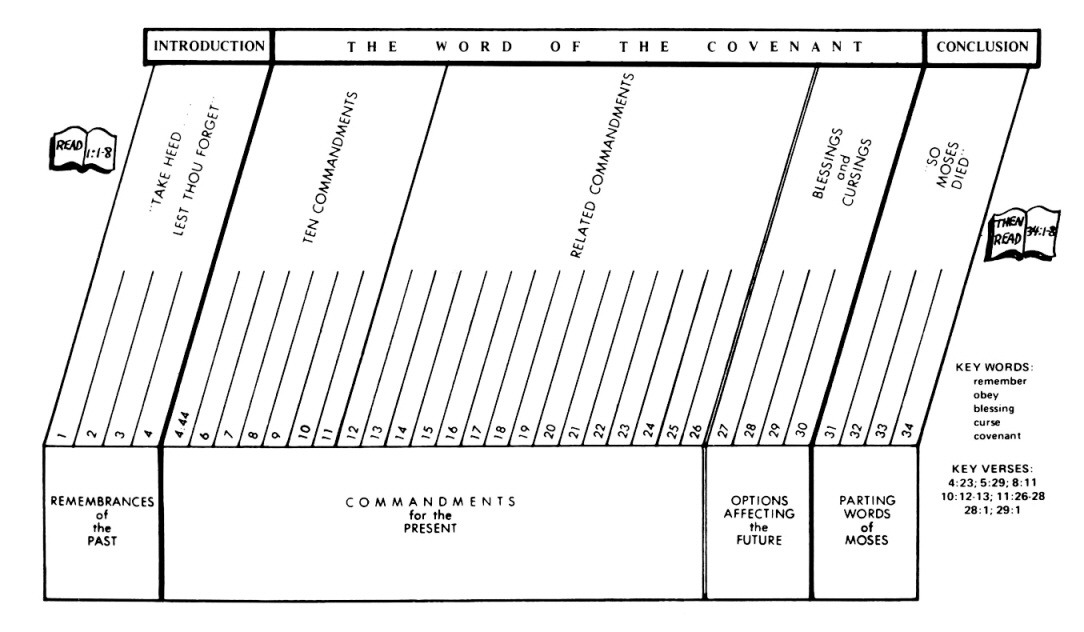
\includegraphics[scale=2.2, angle=90]{05OT-Deuteronomy/References/JensenDeuteronomy.png}
\caption[Deuteronomy by Jensen]{Deuteronomy by Jensen}
\label{fig:Deuteronomy by Jensen}
\end{center}
\end{figure}

\newpage
\begin{figure}
\begin{center}
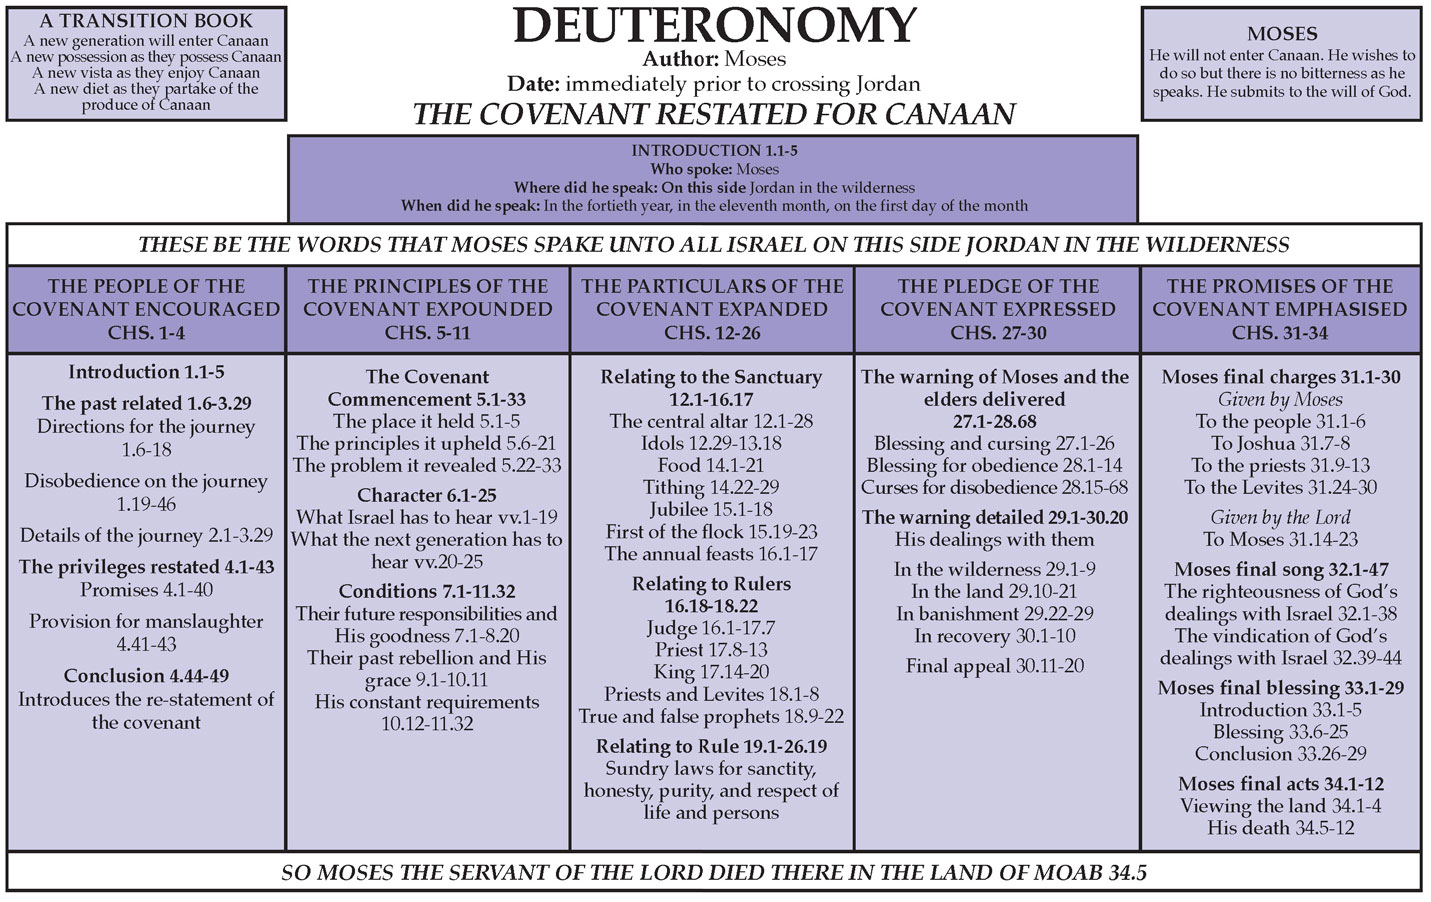
\includegraphics[scale=0.4, angle=90]{05OT-Deuteronomy/References/JohnGrantDeuteronomy.jpg}
\caption[Deuteronomy by John Grant]{Deuteronomy by John Grant}
\label{fig:Deuteronomy by John Grant}
\end{center}
\end{figure}

\newpage
\begin{figure}
\begin{center}
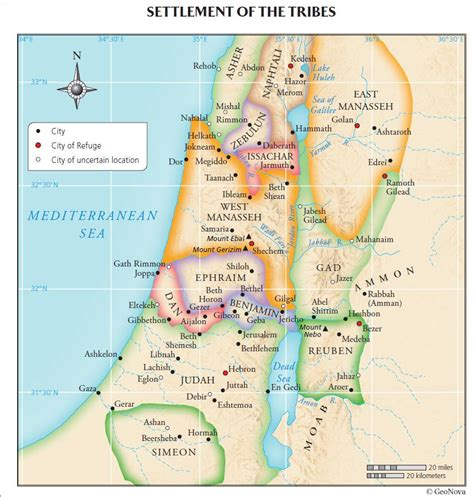
\includegraphics[scale=1, angle=0]{05OT-Deuteronomy/References/SettlementOfTheTribes.jpeg}
\caption[Settlement of the Tribes]{Settlement of the Tribes}
\label{fig:Settlement of the Tribes}
\end{center}
\end{figure}


\newpage
\begin{figure}
\begin{center}
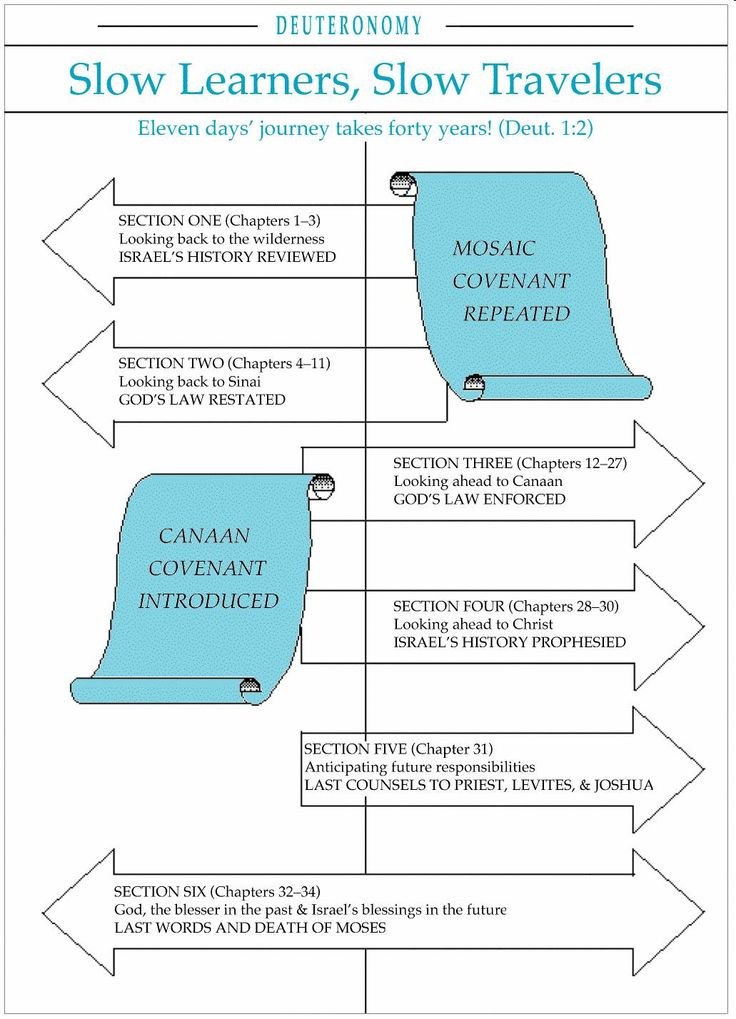
\includegraphics[scale=0.5, angle=0]{05OT-Deuteronomy/References/SlowLearners.jpeg}
\caption[Slow Learners in Deuteronomy]{Slow Learners in Deuteronomy}
\label{fig:Slow Learners in Deuteronomy}
\end{center}
\end{figure}


\newpage
\begin{figure}
\begin{center}
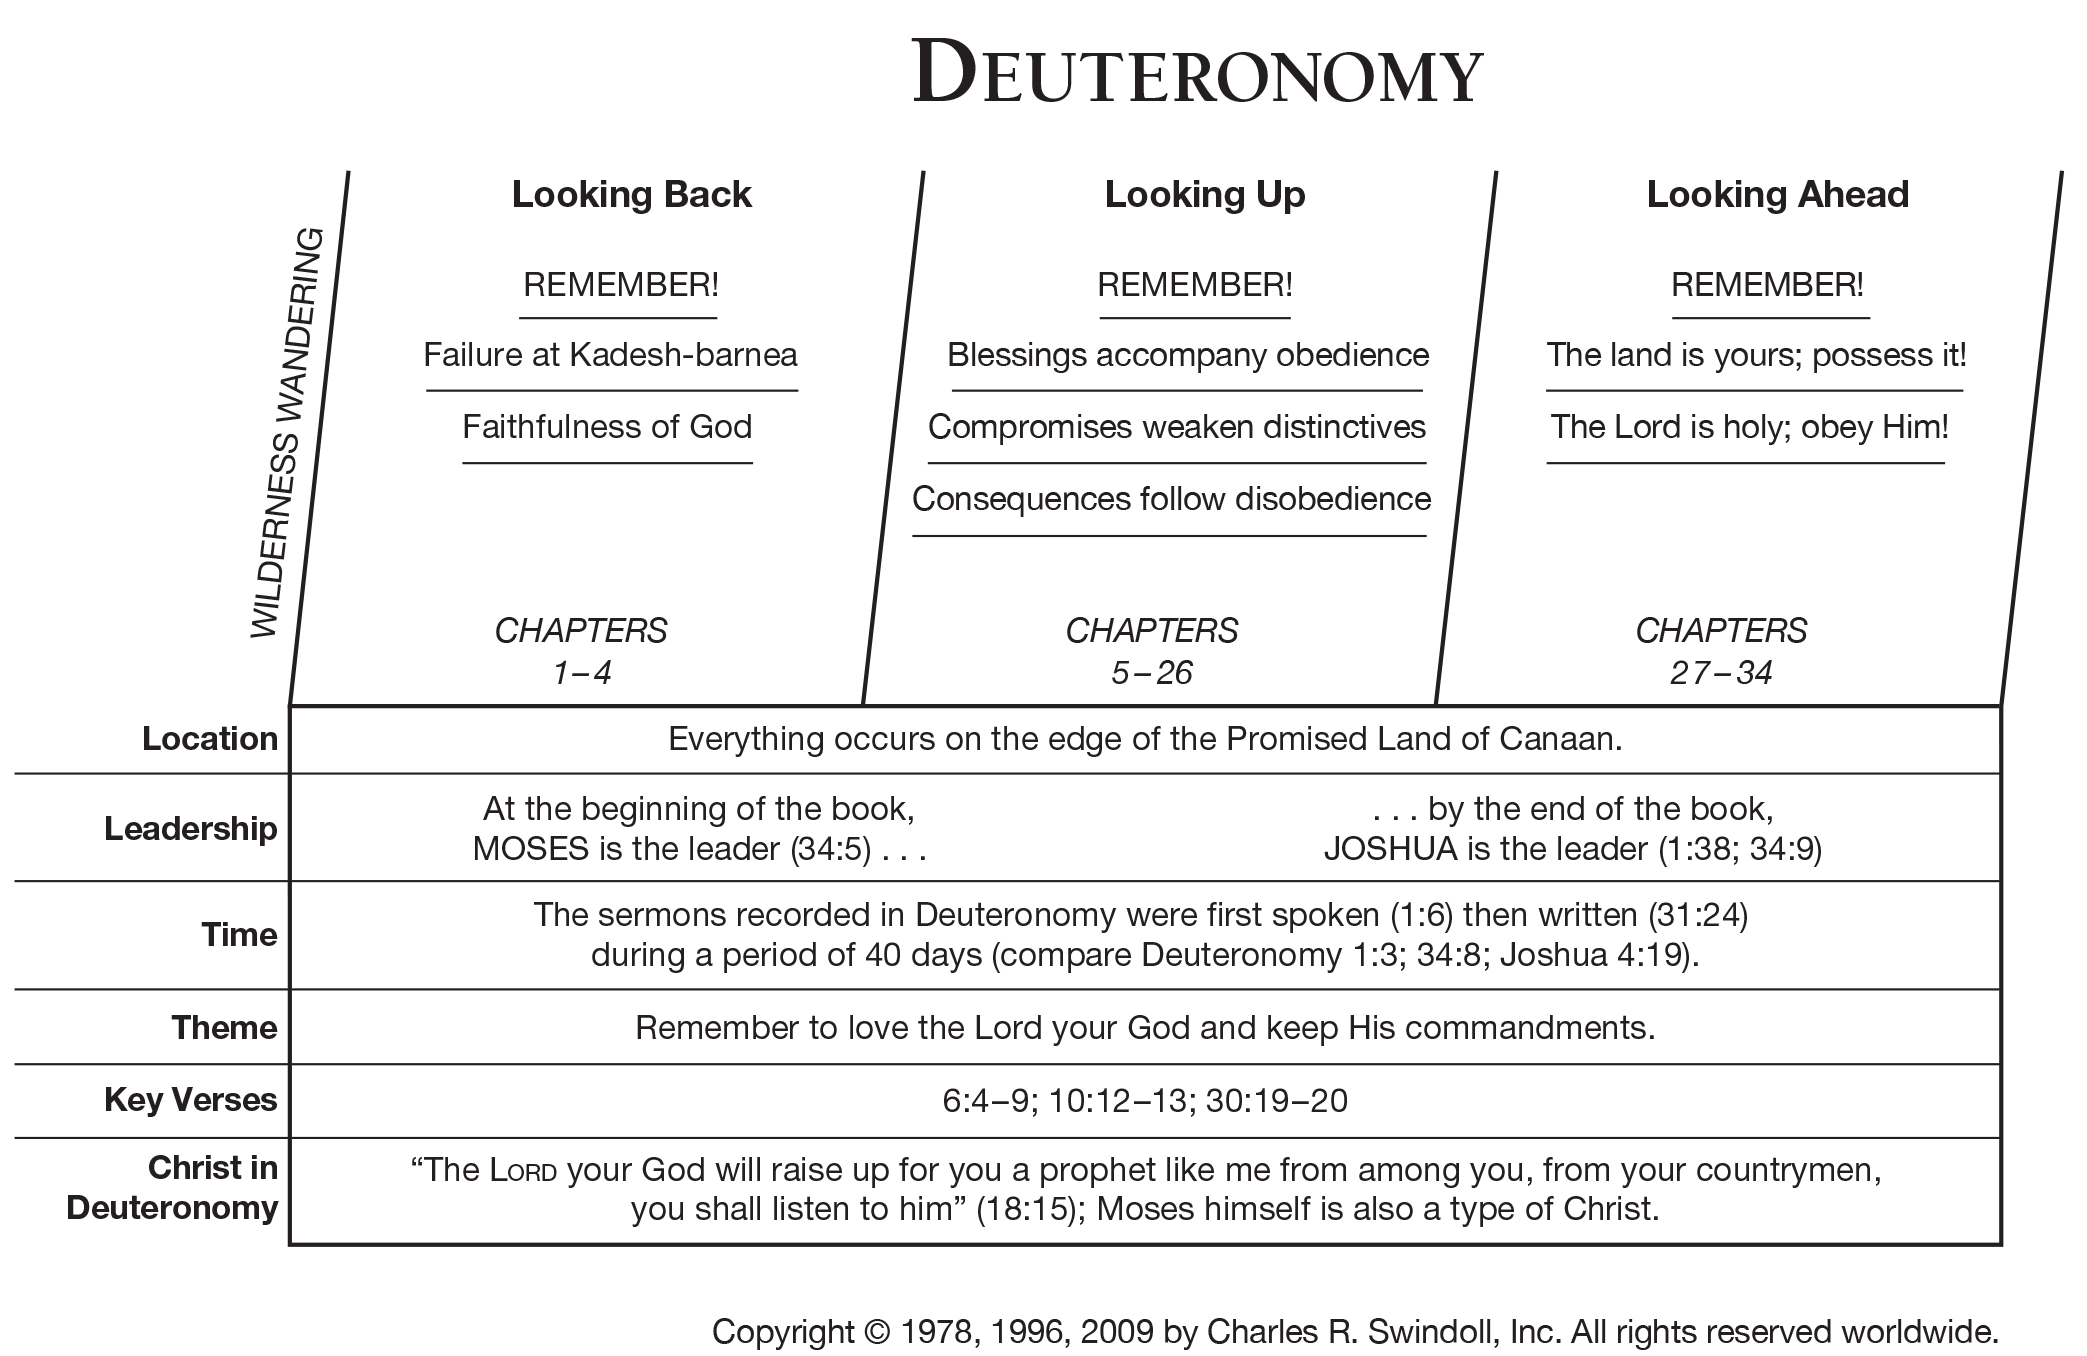
\includegraphics[scale=0.3, angle=90]{05OT-Deuteronomy/References/Swindoll-Deuteronomy.png}
\caption[Deuteronomy by Swindoll]{Deuteronomy by Swindoll}
\label{fig:Deuteronomy by Swindoll}
\end{center}
\end{figure}


\newpage
\begin{figure}
\begin{center}
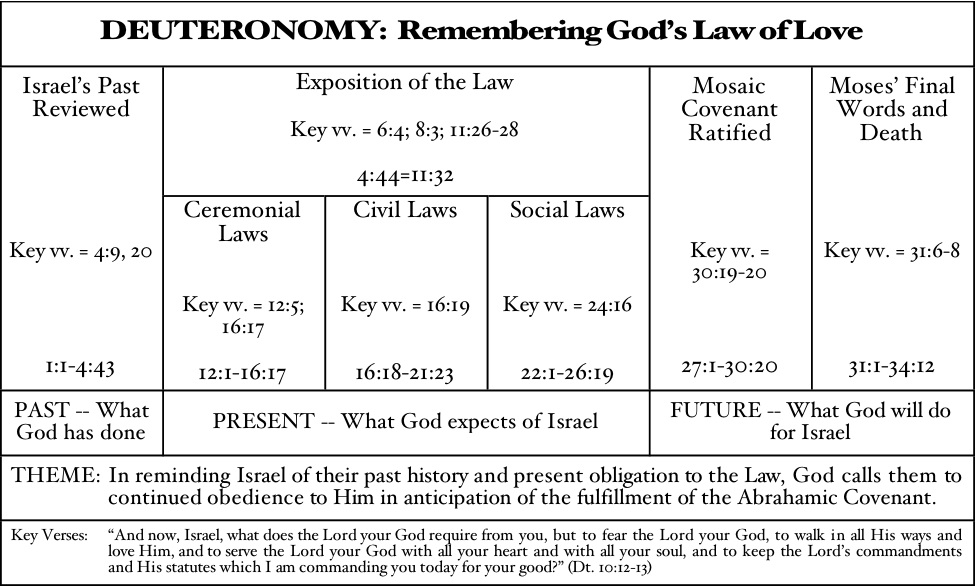
\includegraphics[scale=1, angle=90]{05OT-Deuteronomy/References/WordsOfGrace-Deuteronomy.jpg}
\caption[Deuteronomy from Words of Grace]{Deuteronomy from Words of Grace}
\label{fig:Deuteronomy from Words of Grace}
\end{center}
\end{figure}






\chapter{Deuteronomy 7}

\marginpar{\scriptsize \centering \fcolorbox{black}{lime}{\textbf{7 NATIONS TARGETED}}\\ (Deuteronomy 7:1-26) \begin{compactenum}[I.][8]
    \item  \textbf{Finally at the Land} \index[scripture]{Deuteronomy!Deu 07:01} (Deu 7:1)
    \item  \textbf{Foreigners Left Alone} \index[scripture]{Deuteronomy!Deu 07:03} (Deu 7:3)
    \item  No \textbf{Favor to the Locals} \index[scripture]{Deuteronomy!Deu 07:05} (Deu 7:5)
	\item  The \textbf{Faithfulness of the Lord} \index[scripture]{Deuteronomy!Deu 07:09} (Deu 7:9)
    \item  \textbf{Fear to be Lacking}
    \item  \textbf{False gods Eliminated} %\index[scripture]{Deuteronomy!Deu 07:21} (Deuteronomy 7:21)
    \item  \textbf{Fires Lit} \index[scripture]{Deuteronomy!Deu 07:05}\index[scripture]{Deuteronomy!Deu 07:25} (Deu 7:5, 25)
\end{compactenum}}

\footnote{\textcolor[cmyk]{0.99998,1,0,0}{\hyperlink{TOC}{Return to end of Table of Contents.}}}\footnote{\href{https://audiobible.com/bible/deuteronomy_7.html}{\textcolor[cmyk]{0.99998,1,0,0}{Deuteronomy 7 Audio}}}\textcolor[cmyk]{0.99998,1,0,0}{\fcolorbox{black}{lime}{When} the LORD thy God shall bring thee into the land whither thou goest \fcolorbox{bone}{bone}{to}possess it, and hath cast out many nations before thee, the Hittites, and the Girgashites, and the Amorites, and the Canaanites, and the Perizzites, and the Hivites, and the Jebusites, seven nations greater and mightier than thou;}\marginpar{\scriptsize \textcolor[rgb]{0.00,0.545,0.269}{$\rightarrow$The List of 7 nations: 
\begin{compactenum}
	\item Hittites
	\item Girgashites
	\item Amorites
	\item Canaanites
	\item Perizzites
	\item Hivites
	\item Jebusites
\end{compactenum}}}
[2] \textcolor[cmyk]{0.99998,1,0,0}{And when the LORD thy God shall deliver them before thee; thou shalt smite them, \emph{and} utterly destroy them; thou shalt make no covenant with them, nor shew mercy unto them:}
[3] \textcolor[cmyk]{0.99998,1,0,0}{\fcolorbox{black}{lime}{Neither} shalt thou make marriages with them; thy daughter thou shalt not give unto his son, nor his daughter shalt thou take unto thy son.}
[4] \textcolor[cmyk]{0.99998,1,0,0}{For they will turn away thy son from following me, that they may serve other gods: so will the anger of the LORD be kindled against you, and destroy thee suddenly.}
[5] \textcolor[cmyk]{0.99998,1,0,0}{But thus shall ye deal with them; ye shall \fcolorbox{black}{lime}{destroy} their altars, and \fcolorbox{black}{lime}{break} down their images, and \fcolorbox{black}{lime}{cut down} their groves, and \fcolorbox{black}{lime}{burn} their graven images with fire.}
[6] \textcolor[cmyk]{0.99998,1,0,0}{For thou \emph{art} an holy people unto the LORD thy God: the LORD thy God hath chosen thee \fcolorbox{bone}{bone}{to}be a special people unto himself, above all people that \emph{are} upon the face of the earth.}
[7] \textcolor[cmyk]{0.99998,1,0,0}{The LORD did not set his love upon you, nor choose you, because ye were more in number than any people; for ye \emph{were} the fewest of all people:}
[8] \textcolor[cmyk]{0.99998,1,0,0}{But because the LORD loved you, and because he would keep the oath which he had sworn unto your fathers, hath the LORD brought you out with a mighty hand, and redeemed you out of the house of bondmen, from the hand of Pharaoh king of Egypt.}
[9] \textcolor[cmyk]{0.99998,1,0,0}{Know therefore that the LORD thy God, he \emph{is} God, the \fcolorbox{black}{lime}{faithful} God, which keepeth covenant and mercy with them that love him and keep his commandments \fcolorbox{bone}{bone}{to}a thousand generations;}
[10] \textcolor[cmyk]{0.99998,1,0,0}{And repayeth them that hate him \fcolorbox{bone}{bone}{to}their face, \fcolorbox{bone}{bone}{to}destroy them: he will not be slack \fcolorbox{bone}{bone}{to}him that hateth him, he will repay him \fcolorbox{bone}{bone}{to}his face.}
[11] \textcolor[cmyk]{0.99998,1,0,0}{Thou shalt therefore keep the commandments, and the statutes, and the judgments, which I command thee this day, \fcolorbox{bone}{bone}{to}do them.}\\
\\
\P \textcolor[cmyk]{0.99998,1,0,0}{Wherefore it shall come \fcolorbox{bone}{bone}{to}pass, if ye hearken \fcolorbox{bone}{bone}{to}these judgments, and keep, and do them, that the LORD thy God shall keep unto thee the covenant and the mercy which he sware unto thy fathers:}
[13] \textcolor[cmyk]{0.99998,1,0,0}{And he will love thee, and bless thee, and multiply thee: he will also bless the fruit of thy womb, and the fruit of thy land, thy corn, and thy wine, and thine oil, the increase of thy kine, and the flocks of thy sheep, in the land which he sware unto thy fathers \fcolorbox{bone}{bone}{to}give thee.}
[14] \textcolor[cmyk]{0.99998,1,0,0}{Thou shalt be blessed above all people: there shall not be male or female barren among you, or among your cattle.}
[15] \textcolor[cmyk]{0.99998,1,0,0}{And the LORD will take away from thee all sickness, and will put none of the evil diseases of Egypt, which thou knowest, upon thee; but will lay them upon all \emph{them} that hate thee.}
[16] \textcolor[cmyk]{0.99998,1,0,0}{And thou shalt consume all the people which the LORD thy God shall deliver thee; thine eye shall have no pity upon them: neither shalt thou serve their gods; for that \emph{will} \emph{be} a snare unto thee.}
[17] \textcolor[cmyk]{0.99998,1,0,0}{If thou shalt say in thine heart, These nations \emph{are} more than I; how can I dispossess them?}
[18] \textcolor[cmyk]{0.99998,1,0,0}{Thou shalt not be afraid of them: \emph{but} shalt well remember what the LORD thy God did unto Pharaoh, and unto all Egypt;}
[19] \textcolor[cmyk]{0.99998,1,0,0}{The great temptations which thine eyes saw, and the signs, and the wonders, and the mighty hand, and the stretched out arm, whereby the LORD thy God brought thee out: so shall the LORD thy God do unto all the people of whom thou art afraid.}
[20] \textcolor[cmyk]{0.99998,1,0,0}{Moreover the LORD thy God will send the hornet among them, until they that are left, and hide themselves from thee, be destroyed.}
[21] \textcolor[cmyk]{0.99998,1,0,0}{Thou shalt not be affrighted at them: for the LORD thy God \emph{is} among you, a mighty God and terrible.}
[22] \textcolor[cmyk]{0.99998,1,0,0}{And the LORD thy God will put out those nations before thee by little and little: thou mayest not consume them at once, lest the beasts of the field increase upon thee.}
[23] \textcolor[cmyk]{0.99998,1,0,0}{But the LORD thy God shall deliver them unto thee, and shall destroy them with a mighty destruction, until they be destroyed.}
[24] \textcolor[cmyk]{0.99998,1,0,0}{And he shall deliver their kings into thine hand, and thou shalt destroy their name from under heaven: there shall no man be able \fcolorbox{bone}{bone}{to}stand before thee, until thou have destroyed them.}
[25] \textcolor[cmyk]{0.99998,1,0,0}{The graven images of their gods shall ye burn with fire: thou shalt not desire the silver or gold \emph{that} \emph{is} on them, nor take \emph{it} unto thee, lest thou be snared therein: for it \emph{is} an abomination \fcolorbox{bone}{bone}{to}the LORD thy God.}
[26] \textcolor[cmyk]{0.99998,1,0,0}{Neither shalt thou bring an abomination into thine house, lest thou be a cursed thing like it: \emph{but} thou shalt utterly detest it, and thou shalt utterly abhor it; for it \emph{is} a cursed thing.}
\index[NWIV]{52!Deuteronomy!Deu 7:1}\index[AWIP]{When!Deuteronomy!Deu 7:1}\index[AWIP]{the!Deuteronomy!Deu 7:1}\index[AWIP]{the!Deuteronomy!Deu 7:1 (2)}\index[AWIP]{the!Deuteronomy!Deu 7:1 (3)}\index[AWIP]{the!Deuteronomy!Deu 7:1 (4)}\index[AWIP]{the!Deuteronomy!Deu 7:1 (5)}\index[AWIP]{the!Deuteronomy!Deu 7:1 (6)}\index[AWIP]{the!Deuteronomy!Deu 7:1 (7)}\index[AWIP]{the!Deuteronomy!Deu 7:1 (8)}\index[AWIP]{the!Deuteronomy!Deu 7:1 (9)}\index[AWIP]{LORD!Deuteronomy!Deu 7:1}\index[AWIP]{thy!Deuteronomy!Deu 7:1}\index[AWIP]{God!Deuteronomy!Deu 7:1}\index[AWIP]{shall!Deuteronomy!Deu 7:1}\index[AWIP]{bring!Deuteronomy!Deu 7:1}\index[AWIP]{thee!Deuteronomy!Deu 7:1}\index[AWIP]{thee!Deuteronomy!Deu 7:1 (2)}\index[AWIP]{into!Deuteronomy!Deu 7:1}\index[AWIP]{land!Deuteronomy!Deu 7:1}\index[AWIP]{whither!Deuteronomy!Deu 7:1}\index[AWIP]{thou!Deuteronomy!Deu 7:1}\index[AWIP]{thou!Deuteronomy!Deu 7:1 (2)}\index[AWIP]{goest!Deuteronomy!Deu 7:1}\index[AWIP]{to!Deuteronomy!Deu 7:1}\index[AWIP]{possess!Deuteronomy!Deu 7:1}\index[AWIP]{it!Deuteronomy!Deu 7:1}\index[AWIP]{and!Deuteronomy!Deu 7:1}\index[AWIP]{and!Deuteronomy!Deu 7:1 (2)}\index[AWIP]{and!Deuteronomy!Deu 7:1 (3)}\index[AWIP]{and!Deuteronomy!Deu 7:1 (4)}\index[AWIP]{and!Deuteronomy!Deu 7:1 (5)}\index[AWIP]{and!Deuteronomy!Deu 7:1 (6)}\index[AWIP]{and!Deuteronomy!Deu 7:1 (7)}\index[AWIP]{and!Deuteronomy!Deu 7:1 (8)}\index[AWIP]{hath!Deuteronomy!Deu 7:1}\index[AWIP]{cast!Deuteronomy!Deu 7:1}\index[AWIP]{out!Deuteronomy!Deu 7:1}\index[AWIP]{many!Deuteronomy!Deu 7:1}\index[AWIP]{nations!Deuteronomy!Deu 7:1}\index[AWIP]{nations!Deuteronomy!Deu 7:1 (2)}\index[AWIP]{before!Deuteronomy!Deu 7:1}\index[AWIP]{Hittites!Deuteronomy!Deu 7:1}\index[AWIP]{Girgashites!Deuteronomy!Deu 7:1}\index[AWIP]{Amorites!Deuteronomy!Deu 7:1}\index[AWIP]{Canaanites!Deuteronomy!Deu 7:1}\index[AWIP]{Perizzites!Deuteronomy!Deu 7:1}\index[AWIP]{Hivites!Deuteronomy!Deu 7:1}\index[AWIP]{Jebusites!Deuteronomy!Deu 7:1}\index[AWIP]{seven!Deuteronomy!Deu 7:1}\index[AWIP]{greater!Deuteronomy!Deu 7:1}\index[AWIP]{mightier!Deuteronomy!Deu 7:1}\index[AWIP]{than!Deuteronomy!Deu 7:1}

\index[NWIV]{31!Deuteronomy!Deu 7:2}\index[AWIP]{And!Deuteronomy!Deu 7:2}\index[AWIP]{when!Deuteronomy!Deu 7:2}\index[AWIP]{the!Deuteronomy!Deu 7:2}\index[AWIP]{LORD!Deuteronomy!Deu 7:2}\index[AWIP]{thy!Deuteronomy!Deu 7:2}\index[AWIP]{God!Deuteronomy!Deu 7:2}\index[AWIP]{shall!Deuteronomy!Deu 7:2}\index[AWIP]{deliver!Deuteronomy!Deu 7:2}\index[AWIP]{them!Deuteronomy!Deu 7:2}\index[AWIP]{them!Deuteronomy!Deu 7:2 (2)}\index[AWIP]{them!Deuteronomy!Deu 7:2 (3)}\index[AWIP]{them!Deuteronomy!Deu 7:2 (4)}\index[AWIP]{them!Deuteronomy!Deu 7:2 (5)}\index[AWIP]{before!Deuteronomy!Deu 7:2}\index[AWIP]{thee!Deuteronomy!Deu 7:2}\index[AWIP]{thou!Deuteronomy!Deu 7:2}\index[AWIP]{thou!Deuteronomy!Deu 7:2 (2)}\index[AWIP]{shalt!Deuteronomy!Deu 7:2}\index[AWIP]{shalt!Deuteronomy!Deu 7:2 (2)}\index[AWIP]{smite!Deuteronomy!Deu 7:2}\index[AWIP]{\emph{and}!Deuteronomy!Deu 7:2}\index[AWIP]{utterly!Deuteronomy!Deu 7:2}\index[AWIP]{destroy!Deuteronomy!Deu 7:2}\index[AWIP]{make!Deuteronomy!Deu 7:2}\index[AWIP]{no!Deuteronomy!Deu 7:2}\index[AWIP]{covenant!Deuteronomy!Deu 7:2}\index[AWIP]{with!Deuteronomy!Deu 7:2}\index[AWIP]{nor!Deuteronomy!Deu 7:2}\index[AWIP]{shew!Deuteronomy!Deu 7:2}\index[AWIP]{mercy!Deuteronomy!Deu 7:2}\index[AWIP]{unto!Deuteronomy!Deu 7:2}\index[AWIP]{\emph{and}!Deuteronomy!Deu 7:2}

\index[NWIV]{25!Deuteronomy!Deu 7:3}\index[AWIP]{Neither!Deuteronomy!Deu 7:3}\index[AWIP]{shalt!Deuteronomy!Deu 7:3}\index[AWIP]{shalt!Deuteronomy!Deu 7:3 (2)}\index[AWIP]{shalt!Deuteronomy!Deu 7:3 (3)}\index[AWIP]{thou!Deuteronomy!Deu 7:3}\index[AWIP]{thou!Deuteronomy!Deu 7:3 (2)}\index[AWIP]{thou!Deuteronomy!Deu 7:3 (3)}\index[AWIP]{make!Deuteronomy!Deu 7:3}\index[AWIP]{marriages!Deuteronomy!Deu 7:3}\index[AWIP]{with!Deuteronomy!Deu 7:3}\index[AWIP]{them!Deuteronomy!Deu 7:3}\index[AWIP]{thy!Deuteronomy!Deu 7:3}\index[AWIP]{thy!Deuteronomy!Deu 7:3 (2)}\index[AWIP]{daughter!Deuteronomy!Deu 7:3}\index[AWIP]{daughter!Deuteronomy!Deu 7:3 (2)}\index[AWIP]{not!Deuteronomy!Deu 7:3}\index[AWIP]{give!Deuteronomy!Deu 7:3}\index[AWIP]{unto!Deuteronomy!Deu 7:3}\index[AWIP]{unto!Deuteronomy!Deu 7:3 (2)}\index[AWIP]{his!Deuteronomy!Deu 7:3}\index[AWIP]{his!Deuteronomy!Deu 7:3 (2)}\index[AWIP]{son!Deuteronomy!Deu 7:3}\index[AWIP]{son!Deuteronomy!Deu 7:3 (2)}\index[AWIP]{nor!Deuteronomy!Deu 7:3}\index[AWIP]{take!Deuteronomy!Deu 7:3}

\index[NWIV]{31!Deuteronomy!Deu 7:4}\index[AWIP]{For!Deuteronomy!Deu 7:4}\index[AWIP]{they!Deuteronomy!Deu 7:4}\index[AWIP]{they!Deuteronomy!Deu 7:4 (2)}\index[AWIP]{will!Deuteronomy!Deu 7:4}\index[AWIP]{will!Deuteronomy!Deu 7:4 (2)}\index[AWIP]{turn!Deuteronomy!Deu 7:4}\index[AWIP]{away!Deuteronomy!Deu 7:4}\index[AWIP]{thy!Deuteronomy!Deu 7:4}\index[AWIP]{son!Deuteronomy!Deu 7:4}\index[AWIP]{from!Deuteronomy!Deu 7:4}\index[AWIP]{following!Deuteronomy!Deu 7:4}\index[AWIP]{me!Deuteronomy!Deu 7:4}\index[AWIP]{that!Deuteronomy!Deu 7:4}\index[AWIP]{may!Deuteronomy!Deu 7:4}\index[AWIP]{serve!Deuteronomy!Deu 7:4}\index[AWIP]{other!Deuteronomy!Deu 7:4}\index[AWIP]{gods!Deuteronomy!Deu 7:4}\index[AWIP]{so!Deuteronomy!Deu 7:4}\index[AWIP]{the!Deuteronomy!Deu 7:4}\index[AWIP]{the!Deuteronomy!Deu 7:4 (2)}\index[AWIP]{anger!Deuteronomy!Deu 7:4}\index[AWIP]{of!Deuteronomy!Deu 7:4}\index[AWIP]{LORD!Deuteronomy!Deu 7:4}\index[AWIP]{be!Deuteronomy!Deu 7:4}\index[AWIP]{kindled!Deuteronomy!Deu 7:4}\index[AWIP]{against!Deuteronomy!Deu 7:4}\index[AWIP]{you!Deuteronomy!Deu 7:4}\index[AWIP]{and!Deuteronomy!Deu 7:4}\index[AWIP]{destroy!Deuteronomy!Deu 7:4}\index[AWIP]{thee!Deuteronomy!Deu 7:4}\index[AWIP]{suddenly!Deuteronomy!Deu 7:4}

\index[NWIV]{29!Deuteronomy!Deu 7:5}\index[AWIP]{But!Deuteronomy!Deu 7:5}\index[AWIP]{thus!Deuteronomy!Deu 7:5}\index[AWIP]{shall!Deuteronomy!Deu 7:5}\index[AWIP]{shall!Deuteronomy!Deu 7:5 (2)}\index[AWIP]{ye!Deuteronomy!Deu 7:5}\index[AWIP]{ye!Deuteronomy!Deu 7:5 (2)}\index[AWIP]{deal!Deuteronomy!Deu 7:5}\index[AWIP]{with!Deuteronomy!Deu 7:5}\index[AWIP]{with!Deuteronomy!Deu 7:5 (2)}\index[AWIP]{them!Deuteronomy!Deu 7:5}\index[AWIP]{destroy!Deuteronomy!Deu 7:5}\index[AWIP]{their!Deuteronomy!Deu 7:5}\index[AWIP]{their!Deuteronomy!Deu 7:5 (2)}\index[AWIP]{their!Deuteronomy!Deu 7:5 (3)}\index[AWIP]{their!Deuteronomy!Deu 7:5 (4)}\index[AWIP]{altars!Deuteronomy!Deu 7:5}\index[AWIP]{and!Deuteronomy!Deu 7:5}\index[AWIP]{and!Deuteronomy!Deu 7:5 (2)}\index[AWIP]{and!Deuteronomy!Deu 7:5 (3)}\index[AWIP]{break!Deuteronomy!Deu 7:5}\index[AWIP]{down!Deuteronomy!Deu 7:5}\index[AWIP]{down!Deuteronomy!Deu 7:5 (2)}\index[AWIP]{images!Deuteronomy!Deu 7:5}\index[AWIP]{images!Deuteronomy!Deu 7:5 (2)}\index[AWIP]{cut!Deuteronomy!Deu 7:5}\index[AWIP]{groves!Deuteronomy!Deu 7:5}\index[AWIP]{burn!Deuteronomy!Deu 7:5}\index[AWIP]{graven!Deuteronomy!Deu 7:5}\index[AWIP]{fire!Deuteronomy!Deu 7:5}

\index[NWIV]{36!Deuteronomy!Deu 7:6}\index[AWIP]{For!Deuteronomy!Deu 7:6}\index[AWIP]{thou!Deuteronomy!Deu 7:6}\index[AWIP]{\emph{art}!Deuteronomy!Deu 7:6}\index[AWIP]{an!Deuteronomy!Deu 7:6}\index[AWIP]{holy!Deuteronomy!Deu 7:6}\index[AWIP]{people!Deuteronomy!Deu 7:6}\index[AWIP]{people!Deuteronomy!Deu 7:6 (2)}\index[AWIP]{people!Deuteronomy!Deu 7:6 (3)}\index[AWIP]{unto!Deuteronomy!Deu 7:6}\index[AWIP]{unto!Deuteronomy!Deu 7:6 (2)}\index[AWIP]{the!Deuteronomy!Deu 7:6}\index[AWIP]{the!Deuteronomy!Deu 7:6 (2)}\index[AWIP]{the!Deuteronomy!Deu 7:6 (3)}\index[AWIP]{the!Deuteronomy!Deu 7:6 (4)}\index[AWIP]{LORD!Deuteronomy!Deu 7:6}\index[AWIP]{LORD!Deuteronomy!Deu 7:6 (2)}\index[AWIP]{thy!Deuteronomy!Deu 7:6}\index[AWIP]{thy!Deuteronomy!Deu 7:6 (2)}\index[AWIP]{God!Deuteronomy!Deu 7:6}\index[AWIP]{God!Deuteronomy!Deu 7:6 (2)}\index[AWIP]{hath!Deuteronomy!Deu 7:6}\index[AWIP]{chosen!Deuteronomy!Deu 7:6}\index[AWIP]{thee!Deuteronomy!Deu 7:6}\index[AWIP]{to!Deuteronomy!Deu 7:6}\index[AWIP]{be!Deuteronomy!Deu 7:6}\index[AWIP]{a!Deuteronomy!Deu 7:6}\index[AWIP]{special!Deuteronomy!Deu 7:6}\index[AWIP]{himself!Deuteronomy!Deu 7:6}\index[AWIP]{above!Deuteronomy!Deu 7:6}\index[AWIP]{all!Deuteronomy!Deu 7:6}\index[AWIP]{that!Deuteronomy!Deu 7:6}\index[AWIP]{\emph{are}!Deuteronomy!Deu 7:6}\index[AWIP]{upon!Deuteronomy!Deu 7:6}\index[AWIP]{face!Deuteronomy!Deu 7:6}\index[AWIP]{of!Deuteronomy!Deu 7:6}\index[AWIP]{earth!Deuteronomy!Deu 7:6}\index[AWIP]{\emph{art}!Deuteronomy!Deu 7:6}\index[AWIP]{\emph{are}!Deuteronomy!Deu 7:6}

\index[NWIV]{29!Deuteronomy!Deu 7:7}\index[AWIP]{The!Deuteronomy!Deu 7:7}\index[AWIP]{LORD!Deuteronomy!Deu 7:7}\index[AWIP]{did!Deuteronomy!Deu 7:7}\index[AWIP]{not!Deuteronomy!Deu 7:7}\index[AWIP]{set!Deuteronomy!Deu 7:7}\index[AWIP]{his!Deuteronomy!Deu 7:7}\index[AWIP]{love!Deuteronomy!Deu 7:7}\index[AWIP]{upon!Deuteronomy!Deu 7:7}\index[AWIP]{you!Deuteronomy!Deu 7:7}\index[AWIP]{you!Deuteronomy!Deu 7:7 (2)}\index[AWIP]{nor!Deuteronomy!Deu 7:7}\index[AWIP]{choose!Deuteronomy!Deu 7:7}\index[AWIP]{because!Deuteronomy!Deu 7:7}\index[AWIP]{ye!Deuteronomy!Deu 7:7}\index[AWIP]{ye!Deuteronomy!Deu 7:7 (2)}\index[AWIP]{were!Deuteronomy!Deu 7:7}\index[AWIP]{more!Deuteronomy!Deu 7:7}\index[AWIP]{in!Deuteronomy!Deu 7:7}\index[AWIP]{number!Deuteronomy!Deu 7:7}\index[AWIP]{than!Deuteronomy!Deu 7:7}\index[AWIP]{any!Deuteronomy!Deu 7:7}\index[AWIP]{people!Deuteronomy!Deu 7:7}\index[AWIP]{people!Deuteronomy!Deu 7:7 (2)}\index[AWIP]{for!Deuteronomy!Deu 7:7}\index[AWIP]{\emph{were}!Deuteronomy!Deu 7:7}\index[AWIP]{the!Deuteronomy!Deu 7:7}\index[AWIP]{fewest!Deuteronomy!Deu 7:7}\index[AWIP]{of!Deuteronomy!Deu 7:7}\index[AWIP]{all!Deuteronomy!Deu 7:7}\index[AWIP]{\emph{were}!Deuteronomy!Deu 7:7}

\index[NWIV]{47!Deuteronomy!Deu 7:8}\index[AWIP]{But!Deuteronomy!Deu 7:8}\index[AWIP]{because!Deuteronomy!Deu 7:8}\index[AWIP]{because!Deuteronomy!Deu 7:8 (2)}\index[AWIP]{the!Deuteronomy!Deu 7:8}\index[AWIP]{the!Deuteronomy!Deu 7:8 (2)}\index[AWIP]{the!Deuteronomy!Deu 7:8 (3)}\index[AWIP]{the!Deuteronomy!Deu 7:8 (4)}\index[AWIP]{the!Deuteronomy!Deu 7:8 (5)}\index[AWIP]{LORD!Deuteronomy!Deu 7:8}\index[AWIP]{LORD!Deuteronomy!Deu 7:8 (2)}\index[AWIP]{loved!Deuteronomy!Deu 7:8}\index[AWIP]{you!Deuteronomy!Deu 7:8}\index[AWIP]{you!Deuteronomy!Deu 7:8 (2)}\index[AWIP]{you!Deuteronomy!Deu 7:8 (3)}\index[AWIP]{and!Deuteronomy!Deu 7:8}\index[AWIP]{and!Deuteronomy!Deu 7:8 (2)}\index[AWIP]{he!Deuteronomy!Deu 7:8}\index[AWIP]{he!Deuteronomy!Deu 7:8 (2)}\index[AWIP]{would!Deuteronomy!Deu 7:8}\index[AWIP]{keep!Deuteronomy!Deu 7:8}\index[AWIP]{oath!Deuteronomy!Deu 7:8}\index[AWIP]{which!Deuteronomy!Deu 7:8}\index[AWIP]{had!Deuteronomy!Deu 7:8}\index[AWIP]{sworn!Deuteronomy!Deu 7:8}\index[AWIP]{unto!Deuteronomy!Deu 7:8}\index[AWIP]{your!Deuteronomy!Deu 7:8}\index[AWIP]{fathers!Deuteronomy!Deu 7:8}\index[AWIP]{hath!Deuteronomy!Deu 7:8}\index[AWIP]{brought!Deuteronomy!Deu 7:8}\index[AWIP]{out!Deuteronomy!Deu 7:8}\index[AWIP]{out!Deuteronomy!Deu 7:8 (2)}\index[AWIP]{with!Deuteronomy!Deu 7:8}\index[AWIP]{a!Deuteronomy!Deu 7:8}\index[AWIP]{mighty!Deuteronomy!Deu 7:8}\index[AWIP]{hand!Deuteronomy!Deu 7:8}\index[AWIP]{hand!Deuteronomy!Deu 7:8 (2)}\index[AWIP]{redeemed!Deuteronomy!Deu 7:8}\index[AWIP]{of!Deuteronomy!Deu 7:8}\index[AWIP]{of!Deuteronomy!Deu 7:8 (2)}\index[AWIP]{of!Deuteronomy!Deu 7:8 (3)}\index[AWIP]{of!Deuteronomy!Deu 7:8 (4)}\index[AWIP]{house!Deuteronomy!Deu 7:8}\index[AWIP]{bondmen!Deuteronomy!Deu 7:8}\index[AWIP]{from!Deuteronomy!Deu 7:8}\index[AWIP]{Pharaoh!Deuteronomy!Deu 7:8}\index[AWIP]{king!Deuteronomy!Deu 7:8}\index[AWIP]{Egypt!Deuteronomy!Deu 7:8}

\index[NWIV]{31!Deuteronomy!Deu 7:9}\index[AWIP]{Know!Deuteronomy!Deu 7:9}\index[AWIP]{therefore!Deuteronomy!Deu 7:9}\index[AWIP]{that!Deuteronomy!Deu 7:9}\index[AWIP]{that!Deuteronomy!Deu 7:9 (2)}\index[AWIP]{the!Deuteronomy!Deu 7:9}\index[AWIP]{the!Deuteronomy!Deu 7:9 (2)}\index[AWIP]{LORD!Deuteronomy!Deu 7:9}\index[AWIP]{thy!Deuteronomy!Deu 7:9}\index[AWIP]{God!Deuteronomy!Deu 7:9}\index[AWIP]{God!Deuteronomy!Deu 7:9 (2)}\index[AWIP]{God!Deuteronomy!Deu 7:9 (3)}\index[AWIP]{he!Deuteronomy!Deu 7:9}\index[AWIP]{\emph{is}!Deuteronomy!Deu 7:9}\index[AWIP]{faithful!Deuteronomy!Deu 7:9}\index[AWIP]{which!Deuteronomy!Deu 7:9}\index[AWIP]{keepeth!Deuteronomy!Deu 7:9}\index[AWIP]{covenant!Deuteronomy!Deu 7:9}\index[AWIP]{and!Deuteronomy!Deu 7:9}\index[AWIP]{and!Deuteronomy!Deu 7:9 (2)}\index[AWIP]{mercy!Deuteronomy!Deu 7:9}\index[AWIP]{with!Deuteronomy!Deu 7:9}\index[AWIP]{them!Deuteronomy!Deu 7:9}\index[AWIP]{love!Deuteronomy!Deu 7:9}\index[AWIP]{him!Deuteronomy!Deu 7:9}\index[AWIP]{keep!Deuteronomy!Deu 7:9}\index[AWIP]{his!Deuteronomy!Deu 7:9}\index[AWIP]{commandments!Deuteronomy!Deu 7:9}\index[AWIP]{to!Deuteronomy!Deu 7:9}\index[AWIP]{a!Deuteronomy!Deu 7:9}\index[AWIP]{thousand!Deuteronomy!Deu 7:9}\index[AWIP]{generations!Deuteronomy!Deu 7:9}\index[AWIP]{\emph{is}!Deuteronomy!Deu 7:9}

\index[NWIV]{29!Deuteronomy!Deu 7:10}\index[AWIP]{And!Deuteronomy!Deu 7:10}\index[AWIP]{repayeth!Deuteronomy!Deu 7:10}\index[AWIP]{them!Deuteronomy!Deu 7:10}\index[AWIP]{them!Deuteronomy!Deu 7:10 (2)}\index[AWIP]{that!Deuteronomy!Deu 7:10}\index[AWIP]{that!Deuteronomy!Deu 7:10 (2)}\index[AWIP]{hate!Deuteronomy!Deu 7:10}\index[AWIP]{him!Deuteronomy!Deu 7:10}\index[AWIP]{him!Deuteronomy!Deu 7:10 (2)}\index[AWIP]{him!Deuteronomy!Deu 7:10 (3)}\index[AWIP]{him!Deuteronomy!Deu 7:10 (4)}\index[AWIP]{to!Deuteronomy!Deu 7:10}\index[AWIP]{to!Deuteronomy!Deu 7:10 (2)}\index[AWIP]{to!Deuteronomy!Deu 7:10 (3)}\index[AWIP]{to!Deuteronomy!Deu 7:10 (4)}\index[AWIP]{their!Deuteronomy!Deu 7:10}\index[AWIP]{face!Deuteronomy!Deu 7:10}\index[AWIP]{face!Deuteronomy!Deu 7:10 (2)}\index[AWIP]{destroy!Deuteronomy!Deu 7:10}\index[AWIP]{he!Deuteronomy!Deu 7:10}\index[AWIP]{he!Deuteronomy!Deu 7:10 (2)}\index[AWIP]{will!Deuteronomy!Deu 7:10}\index[AWIP]{will!Deuteronomy!Deu 7:10 (2)}\index[AWIP]{not!Deuteronomy!Deu 7:10}\index[AWIP]{be!Deuteronomy!Deu 7:10}\index[AWIP]{slack!Deuteronomy!Deu 7:10}\index[AWIP]{hateth!Deuteronomy!Deu 7:10}\index[AWIP]{repay!Deuteronomy!Deu 7:10}\index[AWIP]{his!Deuteronomy!Deu 7:10}

\index[NWIV]{21!Deuteronomy!Deu 7:11}\index[AWIP]{Thou!Deuteronomy!Deu 7:11}\index[AWIP]{shalt!Deuteronomy!Deu 7:11}\index[AWIP]{therefore!Deuteronomy!Deu 7:11}\index[AWIP]{keep!Deuteronomy!Deu 7:11}\index[AWIP]{the!Deuteronomy!Deu 7:11}\index[AWIP]{the!Deuteronomy!Deu 7:11 (2)}\index[AWIP]{the!Deuteronomy!Deu 7:11 (3)}\index[AWIP]{commandments!Deuteronomy!Deu 7:11}\index[AWIP]{and!Deuteronomy!Deu 7:11}\index[AWIP]{and!Deuteronomy!Deu 7:11 (2)}\index[AWIP]{statutes!Deuteronomy!Deu 7:11}\index[AWIP]{judgments!Deuteronomy!Deu 7:11}\index[AWIP]{which!Deuteronomy!Deu 7:11}\index[AWIP]{I!Deuteronomy!Deu 7:11}\index[AWIP]{command!Deuteronomy!Deu 7:11}\index[AWIP]{thee!Deuteronomy!Deu 7:11}\index[AWIP]{this!Deuteronomy!Deu 7:11}\index[AWIP]{day!Deuteronomy!Deu 7:11}\index[AWIP]{to!Deuteronomy!Deu 7:11}\index[AWIP]{do!Deuteronomy!Deu 7:11}\index[AWIP]{them!Deuteronomy!Deu 7:11}

\index[NWIV]{37!Deuteronomy!Deu 7:12}\index[AWIP]{Wherefore!Deuteronomy!Deu 7:12}\index[AWIP]{it!Deuteronomy!Deu 7:12}\index[AWIP]{shall!Deuteronomy!Deu 7:12}\index[AWIP]{shall!Deuteronomy!Deu 7:12 (2)}\index[AWIP]{come!Deuteronomy!Deu 7:12}\index[AWIP]{to!Deuteronomy!Deu 7:12}\index[AWIP]{to!Deuteronomy!Deu 7:12 (2)}\index[AWIP]{pass!Deuteronomy!Deu 7:12}\index[AWIP]{if!Deuteronomy!Deu 7:12}\index[AWIP]{ye!Deuteronomy!Deu 7:12}\index[AWIP]{hearken!Deuteronomy!Deu 7:12}\index[AWIP]{these!Deuteronomy!Deu 7:12}\index[AWIP]{judgments!Deuteronomy!Deu 7:12}\index[AWIP]{and!Deuteronomy!Deu 7:12}\index[AWIP]{and!Deuteronomy!Deu 7:12 (2)}\index[AWIP]{and!Deuteronomy!Deu 7:12 (3)}\index[AWIP]{keep!Deuteronomy!Deu 7:12}\index[AWIP]{keep!Deuteronomy!Deu 7:12 (2)}\index[AWIP]{do!Deuteronomy!Deu 7:12}\index[AWIP]{them!Deuteronomy!Deu 7:12}\index[AWIP]{that!Deuteronomy!Deu 7:12}\index[AWIP]{the!Deuteronomy!Deu 7:12}\index[AWIP]{the!Deuteronomy!Deu 7:12 (2)}\index[AWIP]{the!Deuteronomy!Deu 7:12 (3)}\index[AWIP]{LORD!Deuteronomy!Deu 7:12}\index[AWIP]{thy!Deuteronomy!Deu 7:12}\index[AWIP]{thy!Deuteronomy!Deu 7:12 (2)}\index[AWIP]{God!Deuteronomy!Deu 7:12}\index[AWIP]{unto!Deuteronomy!Deu 7:12}\index[AWIP]{unto!Deuteronomy!Deu 7:12 (2)}\index[AWIP]{thee!Deuteronomy!Deu 7:12}\index[AWIP]{covenant!Deuteronomy!Deu 7:12}\index[AWIP]{mercy!Deuteronomy!Deu 7:12}\index[AWIP]{which!Deuteronomy!Deu 7:12}\index[AWIP]{he!Deuteronomy!Deu 7:12}\index[AWIP]{sware!Deuteronomy!Deu 7:12}\index[AWIP]{fathers!Deuteronomy!Deu 7:12}

\index[NWIV]{57!Deuteronomy!Deu 7:13}\index[AWIP]{And!Deuteronomy!Deu 7:13}\index[AWIP]{he!Deuteronomy!Deu 7:13}\index[AWIP]{he!Deuteronomy!Deu 7:13 (2)}\index[AWIP]{he!Deuteronomy!Deu 7:13 (3)}\index[AWIP]{will!Deuteronomy!Deu 7:13}\index[AWIP]{will!Deuteronomy!Deu 7:13 (2)}\index[AWIP]{love!Deuteronomy!Deu 7:13}\index[AWIP]{thee!Deuteronomy!Deu 7:13}\index[AWIP]{thee!Deuteronomy!Deu 7:13 (2)}\index[AWIP]{thee!Deuteronomy!Deu 7:13 (3)}\index[AWIP]{thee!Deuteronomy!Deu 7:13 (4)}\index[AWIP]{and!Deuteronomy!Deu 7:13}\index[AWIP]{and!Deuteronomy!Deu 7:13 (2)}\index[AWIP]{and!Deuteronomy!Deu 7:13 (3)}\index[AWIP]{and!Deuteronomy!Deu 7:13 (4)}\index[AWIP]{and!Deuteronomy!Deu 7:13 (5)}\index[AWIP]{and!Deuteronomy!Deu 7:13 (6)}\index[AWIP]{bless!Deuteronomy!Deu 7:13}\index[AWIP]{bless!Deuteronomy!Deu 7:13 (2)}\index[AWIP]{multiply!Deuteronomy!Deu 7:13}\index[AWIP]{also!Deuteronomy!Deu 7:13}\index[AWIP]{the!Deuteronomy!Deu 7:13}\index[AWIP]{the!Deuteronomy!Deu 7:13 (2)}\index[AWIP]{the!Deuteronomy!Deu 7:13 (3)}\index[AWIP]{the!Deuteronomy!Deu 7:13 (4)}\index[AWIP]{the!Deuteronomy!Deu 7:13 (5)}\index[AWIP]{fruit!Deuteronomy!Deu 7:13}\index[AWIP]{fruit!Deuteronomy!Deu 7:13 (2)}\index[AWIP]{of!Deuteronomy!Deu 7:13}\index[AWIP]{of!Deuteronomy!Deu 7:13 (2)}\index[AWIP]{of!Deuteronomy!Deu 7:13 (3)}\index[AWIP]{of!Deuteronomy!Deu 7:13 (4)}\index[AWIP]{thy!Deuteronomy!Deu 7:13}\index[AWIP]{thy!Deuteronomy!Deu 7:13 (2)}\index[AWIP]{thy!Deuteronomy!Deu 7:13 (3)}\index[AWIP]{thy!Deuteronomy!Deu 7:13 (4)}\index[AWIP]{thy!Deuteronomy!Deu 7:13 (5)}\index[AWIP]{thy!Deuteronomy!Deu 7:13 (6)}\index[AWIP]{thy!Deuteronomy!Deu 7:13 (7)}\index[AWIP]{womb!Deuteronomy!Deu 7:13}\index[AWIP]{land!Deuteronomy!Deu 7:13}\index[AWIP]{land!Deuteronomy!Deu 7:13 (2)}\index[AWIP]{corn!Deuteronomy!Deu 7:13}\index[AWIP]{wine!Deuteronomy!Deu 7:13}\index[AWIP]{thine!Deuteronomy!Deu 7:13}\index[AWIP]{oil!Deuteronomy!Deu 7:13}\index[AWIP]{increase!Deuteronomy!Deu 7:13}\index[AWIP]{kine!Deuteronomy!Deu 7:13}\index[AWIP]{flocks!Deuteronomy!Deu 7:13}\index[AWIP]{sheep!Deuteronomy!Deu 7:13}\index[AWIP]{in!Deuteronomy!Deu 7:13}\index[AWIP]{which!Deuteronomy!Deu 7:13}\index[AWIP]{sware!Deuteronomy!Deu 7:13}\index[AWIP]{unto!Deuteronomy!Deu 7:13}\index[AWIP]{fathers!Deuteronomy!Deu 7:13}\index[AWIP]{to!Deuteronomy!Deu 7:13}\index[AWIP]{give!Deuteronomy!Deu 7:13}

\index[NWIV]{21!Deuteronomy!Deu 7:14}\index[AWIP]{Thou!Deuteronomy!Deu 7:14}\index[AWIP]{shalt!Deuteronomy!Deu 7:14}\index[AWIP]{be!Deuteronomy!Deu 7:14}\index[AWIP]{be!Deuteronomy!Deu 7:14 (2)}\index[AWIP]{blessed!Deuteronomy!Deu 7:14}\index[AWIP]{above!Deuteronomy!Deu 7:14}\index[AWIP]{all!Deuteronomy!Deu 7:14}\index[AWIP]{people!Deuteronomy!Deu 7:14}\index[AWIP]{there!Deuteronomy!Deu 7:14}\index[AWIP]{shall!Deuteronomy!Deu 7:14}\index[AWIP]{not!Deuteronomy!Deu 7:14}\index[AWIP]{male!Deuteronomy!Deu 7:14}\index[AWIP]{or!Deuteronomy!Deu 7:14}\index[AWIP]{or!Deuteronomy!Deu 7:14 (2)}\index[AWIP]{female!Deuteronomy!Deu 7:14}\index[AWIP]{barren!Deuteronomy!Deu 7:14}\index[AWIP]{among!Deuteronomy!Deu 7:14}\index[AWIP]{among!Deuteronomy!Deu 7:14 (2)}\index[AWIP]{you!Deuteronomy!Deu 7:14}\index[AWIP]{your!Deuteronomy!Deu 7:14}\index[AWIP]{cattle!Deuteronomy!Deu 7:14}

\index[NWIV]{35!Deuteronomy!Deu 7:15}\index[AWIP]{And!Deuteronomy!Deu 7:15}\index[AWIP]{the!Deuteronomy!Deu 7:15}\index[AWIP]{the!Deuteronomy!Deu 7:15 (2)}\index[AWIP]{LORD!Deuteronomy!Deu 7:15}\index[AWIP]{will!Deuteronomy!Deu 7:15}\index[AWIP]{will!Deuteronomy!Deu 7:15 (2)}\index[AWIP]{will!Deuteronomy!Deu 7:15 (3)}\index[AWIP]{take!Deuteronomy!Deu 7:15}\index[AWIP]{away!Deuteronomy!Deu 7:15}\index[AWIP]{from!Deuteronomy!Deu 7:15}\index[AWIP]{thee!Deuteronomy!Deu 7:15}\index[AWIP]{thee!Deuteronomy!Deu 7:15 (2)}\index[AWIP]{thee!Deuteronomy!Deu 7:15 (3)}\index[AWIP]{all!Deuteronomy!Deu 7:15}\index[AWIP]{all!Deuteronomy!Deu 7:15 (2)}\index[AWIP]{sickness!Deuteronomy!Deu 7:15}\index[AWIP]{and!Deuteronomy!Deu 7:15}\index[AWIP]{put!Deuteronomy!Deu 7:15}\index[AWIP]{none!Deuteronomy!Deu 7:15}\index[AWIP]{of!Deuteronomy!Deu 7:15}\index[AWIP]{of!Deuteronomy!Deu 7:15 (2)}\index[AWIP]{evil!Deuteronomy!Deu 7:15}\index[AWIP]{diseases!Deuteronomy!Deu 7:15}\index[AWIP]{Egypt!Deuteronomy!Deu 7:15}\index[AWIP]{which!Deuteronomy!Deu 7:15}\index[AWIP]{thou!Deuteronomy!Deu 7:15}\index[AWIP]{knowest!Deuteronomy!Deu 7:15}\index[AWIP]{upon!Deuteronomy!Deu 7:15}\index[AWIP]{upon!Deuteronomy!Deu 7:15 (2)}\index[AWIP]{but!Deuteronomy!Deu 7:15}\index[AWIP]{lay!Deuteronomy!Deu 7:15}\index[AWIP]{them!Deuteronomy!Deu 7:15}\index[AWIP]{\emph{them}!Deuteronomy!Deu 7:15}\index[AWIP]{that!Deuteronomy!Deu 7:15}\index[AWIP]{hate!Deuteronomy!Deu 7:15}\index[AWIP]{\emph{them}!Deuteronomy!Deu 7:15}

\index[NWIV]{37!Deuteronomy!Deu 7:16}\index[AWIP]{And!Deuteronomy!Deu 7:16}\index[AWIP]{thou!Deuteronomy!Deu 7:16}\index[AWIP]{thou!Deuteronomy!Deu 7:16 (2)}\index[AWIP]{shalt!Deuteronomy!Deu 7:16}\index[AWIP]{shalt!Deuteronomy!Deu 7:16 (2)}\index[AWIP]{consume!Deuteronomy!Deu 7:16}\index[AWIP]{all!Deuteronomy!Deu 7:16}\index[AWIP]{the!Deuteronomy!Deu 7:16}\index[AWIP]{the!Deuteronomy!Deu 7:16 (2)}\index[AWIP]{people!Deuteronomy!Deu 7:16}\index[AWIP]{which!Deuteronomy!Deu 7:16}\index[AWIP]{LORD!Deuteronomy!Deu 7:16}\index[AWIP]{thy!Deuteronomy!Deu 7:16}\index[AWIP]{God!Deuteronomy!Deu 7:16}\index[AWIP]{shall!Deuteronomy!Deu 7:16}\index[AWIP]{shall!Deuteronomy!Deu 7:16 (2)}\index[AWIP]{deliver!Deuteronomy!Deu 7:16}\index[AWIP]{thee!Deuteronomy!Deu 7:16}\index[AWIP]{thee!Deuteronomy!Deu 7:16 (2)}\index[AWIP]{thine!Deuteronomy!Deu 7:16}\index[AWIP]{eye!Deuteronomy!Deu 7:16}\index[AWIP]{have!Deuteronomy!Deu 7:16}\index[AWIP]{no!Deuteronomy!Deu 7:16}\index[AWIP]{pity!Deuteronomy!Deu 7:16}\index[AWIP]{upon!Deuteronomy!Deu 7:16}\index[AWIP]{them!Deuteronomy!Deu 7:16}\index[AWIP]{neither!Deuteronomy!Deu 7:16}\index[AWIP]{serve!Deuteronomy!Deu 7:16}\index[AWIP]{their!Deuteronomy!Deu 7:16}\index[AWIP]{gods!Deuteronomy!Deu 7:16}\index[AWIP]{for!Deuteronomy!Deu 7:16}\index[AWIP]{that!Deuteronomy!Deu 7:16}\index[AWIP]{\emph{will}!Deuteronomy!Deu 7:16}\index[AWIP]{\emph{be}!Deuteronomy!Deu 7:16}\index[AWIP]{a!Deuteronomy!Deu 7:16}\index[AWIP]{snare!Deuteronomy!Deu 7:16}\index[AWIP]{unto!Deuteronomy!Deu 7:16}\index[AWIP]{\emph{will}!Deuteronomy!Deu 7:16}\index[AWIP]{\emph{be}!Deuteronomy!Deu 7:16}

\index[NWIV]{18!Deuteronomy!Deu 7:17}\index[AWIP]{If!Deuteronomy!Deu 7:17}\index[AWIP]{thou!Deuteronomy!Deu 7:17}\index[AWIP]{shalt!Deuteronomy!Deu 7:17}\index[AWIP]{say!Deuteronomy!Deu 7:17}\index[AWIP]{in!Deuteronomy!Deu 7:17}\index[AWIP]{thine!Deuteronomy!Deu 7:17}\index[AWIP]{heart!Deuteronomy!Deu 7:17}\index[AWIP]{These!Deuteronomy!Deu 7:17}\index[AWIP]{nations!Deuteronomy!Deu 7:17}\index[AWIP]{\emph{are}!Deuteronomy!Deu 7:17}\index[AWIP]{more!Deuteronomy!Deu 7:17}\index[AWIP]{than!Deuteronomy!Deu 7:17}\index[AWIP]{I!Deuteronomy!Deu 7:17}\index[AWIP]{I!Deuteronomy!Deu 7:17 (2)}\index[AWIP]{how!Deuteronomy!Deu 7:17}\index[AWIP]{can!Deuteronomy!Deu 7:17}\index[AWIP]{dispossess!Deuteronomy!Deu 7:17}\index[AWIP]{them?!Deuteronomy!Deu 7:17}\index[AWIP]{\emph{are}!Deuteronomy!Deu 7:17}

\index[NWIV]{23!Deuteronomy!Deu 7:18}\index[AWIP]{Thou!Deuteronomy!Deu 7:18}\index[AWIP]{shalt!Deuteronomy!Deu 7:18}\index[AWIP]{shalt!Deuteronomy!Deu 7:18 (2)}\index[AWIP]{not!Deuteronomy!Deu 7:18}\index[AWIP]{be!Deuteronomy!Deu 7:18}\index[AWIP]{afraid!Deuteronomy!Deu 7:18}\index[AWIP]{of!Deuteronomy!Deu 7:18}\index[AWIP]{them!Deuteronomy!Deu 7:18}\index[AWIP]{\emph{but}!Deuteronomy!Deu 7:18}\index[AWIP]{well!Deuteronomy!Deu 7:18}\index[AWIP]{remember!Deuteronomy!Deu 7:18}\index[AWIP]{what!Deuteronomy!Deu 7:18}\index[AWIP]{the!Deuteronomy!Deu 7:18}\index[AWIP]{LORD!Deuteronomy!Deu 7:18}\index[AWIP]{thy!Deuteronomy!Deu 7:18}\index[AWIP]{God!Deuteronomy!Deu 7:18}\index[AWIP]{did!Deuteronomy!Deu 7:18}\index[AWIP]{unto!Deuteronomy!Deu 7:18}\index[AWIP]{unto!Deuteronomy!Deu 7:18 (2)}\index[AWIP]{Pharaoh!Deuteronomy!Deu 7:18}\index[AWIP]{and!Deuteronomy!Deu 7:18}\index[AWIP]{all!Deuteronomy!Deu 7:18}\index[AWIP]{Egypt!Deuteronomy!Deu 7:18}\index[AWIP]{\emph{but}!Deuteronomy!Deu 7:18}

\index[NWIV]{46!Deuteronomy!Deu 7:19}\index[AWIP]{The!Deuteronomy!Deu 7:19}\index[AWIP]{great!Deuteronomy!Deu 7:19}\index[AWIP]{temptations!Deuteronomy!Deu 7:19}\index[AWIP]{which!Deuteronomy!Deu 7:19}\index[AWIP]{thine!Deuteronomy!Deu 7:19}\index[AWIP]{eyes!Deuteronomy!Deu 7:19}\index[AWIP]{saw!Deuteronomy!Deu 7:19}\index[AWIP]{and!Deuteronomy!Deu 7:19}\index[AWIP]{and!Deuteronomy!Deu 7:19 (2)}\index[AWIP]{and!Deuteronomy!Deu 7:19 (3)}\index[AWIP]{and!Deuteronomy!Deu 7:19 (4)}\index[AWIP]{the!Deuteronomy!Deu 7:19}\index[AWIP]{the!Deuteronomy!Deu 7:19 (2)}\index[AWIP]{the!Deuteronomy!Deu 7:19 (3)}\index[AWIP]{the!Deuteronomy!Deu 7:19 (4)}\index[AWIP]{the!Deuteronomy!Deu 7:19 (5)}\index[AWIP]{the!Deuteronomy!Deu 7:19 (6)}\index[AWIP]{the!Deuteronomy!Deu 7:19 (7)}\index[AWIP]{signs!Deuteronomy!Deu 7:19}\index[AWIP]{wonders!Deuteronomy!Deu 7:19}\index[AWIP]{mighty!Deuteronomy!Deu 7:19}\index[AWIP]{hand!Deuteronomy!Deu 7:19}\index[AWIP]{stretched!Deuteronomy!Deu 7:19}\index[AWIP]{out!Deuteronomy!Deu 7:19}\index[AWIP]{out!Deuteronomy!Deu 7:19 (2)}\index[AWIP]{arm!Deuteronomy!Deu 7:19}\index[AWIP]{whereby!Deuteronomy!Deu 7:19}\index[AWIP]{LORD!Deuteronomy!Deu 7:19}\index[AWIP]{LORD!Deuteronomy!Deu 7:19 (2)}\index[AWIP]{thy!Deuteronomy!Deu 7:19}\index[AWIP]{thy!Deuteronomy!Deu 7:19 (2)}\index[AWIP]{God!Deuteronomy!Deu 7:19}\index[AWIP]{God!Deuteronomy!Deu 7:19 (2)}\index[AWIP]{brought!Deuteronomy!Deu 7:19}\index[AWIP]{thee!Deuteronomy!Deu 7:19}\index[AWIP]{so!Deuteronomy!Deu 7:19}\index[AWIP]{shall!Deuteronomy!Deu 7:19}\index[AWIP]{do!Deuteronomy!Deu 7:19}\index[AWIP]{unto!Deuteronomy!Deu 7:19}\index[AWIP]{all!Deuteronomy!Deu 7:19}\index[AWIP]{people!Deuteronomy!Deu 7:19}\index[AWIP]{of!Deuteronomy!Deu 7:19}\index[AWIP]{whom!Deuteronomy!Deu 7:19}\index[AWIP]{thou!Deuteronomy!Deu 7:19}\index[AWIP]{art!Deuteronomy!Deu 7:19}\index[AWIP]{afraid!Deuteronomy!Deu 7:19}

\index[NWIV]{23!Deuteronomy!Deu 7:20}\index[AWIP]{Moreover!Deuteronomy!Deu 7:20}\index[AWIP]{the!Deuteronomy!Deu 7:20}\index[AWIP]{the!Deuteronomy!Deu 7:20 (2)}\index[AWIP]{LORD!Deuteronomy!Deu 7:20}\index[AWIP]{thy!Deuteronomy!Deu 7:20}\index[AWIP]{God!Deuteronomy!Deu 7:20}\index[AWIP]{will!Deuteronomy!Deu 7:20}\index[AWIP]{send!Deuteronomy!Deu 7:20}\index[AWIP]{hornet!Deuteronomy!Deu 7:20}\index[AWIP]{among!Deuteronomy!Deu 7:20}\index[AWIP]{them!Deuteronomy!Deu 7:20}\index[AWIP]{until!Deuteronomy!Deu 7:20}\index[AWIP]{they!Deuteronomy!Deu 7:20}\index[AWIP]{that!Deuteronomy!Deu 7:20}\index[AWIP]{are!Deuteronomy!Deu 7:20}\index[AWIP]{left!Deuteronomy!Deu 7:20}\index[AWIP]{and!Deuteronomy!Deu 7:20}\index[AWIP]{hide!Deuteronomy!Deu 7:20}\index[AWIP]{themselves!Deuteronomy!Deu 7:20}\index[AWIP]{from!Deuteronomy!Deu 7:20}\index[AWIP]{thee!Deuteronomy!Deu 7:20}\index[AWIP]{be!Deuteronomy!Deu 7:20}\index[AWIP]{destroyed!Deuteronomy!Deu 7:20}

\index[NWIV]{20!Deuteronomy!Deu 7:21}\index[AWIP]{Thou!Deuteronomy!Deu 7:21}\index[AWIP]{shalt!Deuteronomy!Deu 7:21}\index[AWIP]{not!Deuteronomy!Deu 7:21}\index[AWIP]{be!Deuteronomy!Deu 7:21}\index[AWIP]{affrighted!Deuteronomy!Deu 7:21}\index[AWIP]{at!Deuteronomy!Deu 7:21}\index[AWIP]{them!Deuteronomy!Deu 7:21}\index[AWIP]{for!Deuteronomy!Deu 7:21}\index[AWIP]{the!Deuteronomy!Deu 7:21}\index[AWIP]{LORD!Deuteronomy!Deu 7:21}\index[AWIP]{thy!Deuteronomy!Deu 7:21}\index[AWIP]{God!Deuteronomy!Deu 7:21}\index[AWIP]{God!Deuteronomy!Deu 7:21 (2)}\index[AWIP]{\emph{is}!Deuteronomy!Deu 7:21}\index[AWIP]{among!Deuteronomy!Deu 7:21}\index[AWIP]{you!Deuteronomy!Deu 7:21}\index[AWIP]{a!Deuteronomy!Deu 7:21}\index[AWIP]{mighty!Deuteronomy!Deu 7:21}\index[AWIP]{and!Deuteronomy!Deu 7:21}\index[AWIP]{terrible!Deuteronomy!Deu 7:21}\index[AWIP]{\emph{is}!Deuteronomy!Deu 7:21}

\index[NWIV]{32!Deuteronomy!Deu 7:22}\index[AWIP]{And!Deuteronomy!Deu 7:22}\index[AWIP]{the!Deuteronomy!Deu 7:22}\index[AWIP]{the!Deuteronomy!Deu 7:22 (2)}\index[AWIP]{the!Deuteronomy!Deu 7:22 (3)}\index[AWIP]{LORD!Deuteronomy!Deu 7:22}\index[AWIP]{thy!Deuteronomy!Deu 7:22}\index[AWIP]{God!Deuteronomy!Deu 7:22}\index[AWIP]{will!Deuteronomy!Deu 7:22}\index[AWIP]{put!Deuteronomy!Deu 7:22}\index[AWIP]{out!Deuteronomy!Deu 7:22}\index[AWIP]{those!Deuteronomy!Deu 7:22}\index[AWIP]{nations!Deuteronomy!Deu 7:22}\index[AWIP]{before!Deuteronomy!Deu 7:22}\index[AWIP]{thee!Deuteronomy!Deu 7:22}\index[AWIP]{thee!Deuteronomy!Deu 7:22 (2)}\index[AWIP]{by!Deuteronomy!Deu 7:22}\index[AWIP]{little!Deuteronomy!Deu 7:22}\index[AWIP]{little!Deuteronomy!Deu 7:22 (2)}\index[AWIP]{and!Deuteronomy!Deu 7:22}\index[AWIP]{thou!Deuteronomy!Deu 7:22}\index[AWIP]{mayest!Deuteronomy!Deu 7:22}\index[AWIP]{not!Deuteronomy!Deu 7:22}\index[AWIP]{consume!Deuteronomy!Deu 7:22}\index[AWIP]{them!Deuteronomy!Deu 7:22}\index[AWIP]{at!Deuteronomy!Deu 7:22}\index[AWIP]{once!Deuteronomy!Deu 7:22}\index[AWIP]{lest!Deuteronomy!Deu 7:22}\index[AWIP]{beasts!Deuteronomy!Deu 7:22}\index[AWIP]{of!Deuteronomy!Deu 7:22}\index[AWIP]{field!Deuteronomy!Deu 7:22}\index[AWIP]{increase!Deuteronomy!Deu 7:22}\index[AWIP]{upon!Deuteronomy!Deu 7:22}

\index[NWIV]{22!Deuteronomy!Deu 7:23}\index[AWIP]{But!Deuteronomy!Deu 7:23}\index[AWIP]{the!Deuteronomy!Deu 7:23}\index[AWIP]{LORD!Deuteronomy!Deu 7:23}\index[AWIP]{thy!Deuteronomy!Deu 7:23}\index[AWIP]{God!Deuteronomy!Deu 7:23}\index[AWIP]{shall!Deuteronomy!Deu 7:23}\index[AWIP]{shall!Deuteronomy!Deu 7:23 (2)}\index[AWIP]{deliver!Deuteronomy!Deu 7:23}\index[AWIP]{them!Deuteronomy!Deu 7:23}\index[AWIP]{them!Deuteronomy!Deu 7:23 (2)}\index[AWIP]{unto!Deuteronomy!Deu 7:23}\index[AWIP]{thee!Deuteronomy!Deu 7:23}\index[AWIP]{and!Deuteronomy!Deu 7:23}\index[AWIP]{destroy!Deuteronomy!Deu 7:23}\index[AWIP]{with!Deuteronomy!Deu 7:23}\index[AWIP]{a!Deuteronomy!Deu 7:23}\index[AWIP]{mighty!Deuteronomy!Deu 7:23}\index[AWIP]{destruction!Deuteronomy!Deu 7:23}\index[AWIP]{until!Deuteronomy!Deu 7:23}\index[AWIP]{they!Deuteronomy!Deu 7:23}\index[AWIP]{be!Deuteronomy!Deu 7:23}\index[AWIP]{destroyed!Deuteronomy!Deu 7:23}

\index[NWIV]{33!Deuteronomy!Deu 7:24}\index[AWIP]{And!Deuteronomy!Deu 7:24}\index[AWIP]{he!Deuteronomy!Deu 7:24}\index[AWIP]{shall!Deuteronomy!Deu 7:24}\index[AWIP]{shall!Deuteronomy!Deu 7:24 (2)}\index[AWIP]{deliver!Deuteronomy!Deu 7:24}\index[AWIP]{their!Deuteronomy!Deu 7:24}\index[AWIP]{their!Deuteronomy!Deu 7:24 (2)}\index[AWIP]{kings!Deuteronomy!Deu 7:24}\index[AWIP]{into!Deuteronomy!Deu 7:24}\index[AWIP]{thine!Deuteronomy!Deu 7:24}\index[AWIP]{hand!Deuteronomy!Deu 7:24}\index[AWIP]{and!Deuteronomy!Deu 7:24}\index[AWIP]{thou!Deuteronomy!Deu 7:24}\index[AWIP]{thou!Deuteronomy!Deu 7:24 (2)}\index[AWIP]{shalt!Deuteronomy!Deu 7:24}\index[AWIP]{destroy!Deuteronomy!Deu 7:24}\index[AWIP]{name!Deuteronomy!Deu 7:24}\index[AWIP]{from!Deuteronomy!Deu 7:24}\index[AWIP]{under!Deuteronomy!Deu 7:24}\index[AWIP]{heaven!Deuteronomy!Deu 7:24}\index[AWIP]{there!Deuteronomy!Deu 7:24}\index[AWIP]{no!Deuteronomy!Deu 7:24}\index[AWIP]{man!Deuteronomy!Deu 7:24}\index[AWIP]{be!Deuteronomy!Deu 7:24}\index[AWIP]{able!Deuteronomy!Deu 7:24}\index[AWIP]{to!Deuteronomy!Deu 7:24}\index[AWIP]{stand!Deuteronomy!Deu 7:24}\index[AWIP]{before!Deuteronomy!Deu 7:24}\index[AWIP]{thee!Deuteronomy!Deu 7:24}\index[AWIP]{until!Deuteronomy!Deu 7:24}\index[AWIP]{have!Deuteronomy!Deu 7:24}\index[AWIP]{destroyed!Deuteronomy!Deu 7:24}\index[AWIP]{them!Deuteronomy!Deu 7:24}

\index[NWIV]{43!Deuteronomy!Deu 7:25}\index[AWIP]{The!Deuteronomy!Deu 7:25}\index[AWIP]{graven!Deuteronomy!Deu 7:25}\index[AWIP]{images!Deuteronomy!Deu 7:25}\index[AWIP]{of!Deuteronomy!Deu 7:25}\index[AWIP]{their!Deuteronomy!Deu 7:25}\index[AWIP]{gods!Deuteronomy!Deu 7:25}\index[AWIP]{shall!Deuteronomy!Deu 7:25}\index[AWIP]{ye!Deuteronomy!Deu 7:25}\index[AWIP]{burn!Deuteronomy!Deu 7:25}\index[AWIP]{with!Deuteronomy!Deu 7:25}\index[AWIP]{fire!Deuteronomy!Deu 7:25}\index[AWIP]{thou!Deuteronomy!Deu 7:25}\index[AWIP]{thou!Deuteronomy!Deu 7:25 (2)}\index[AWIP]{shalt!Deuteronomy!Deu 7:25}\index[AWIP]{not!Deuteronomy!Deu 7:25}\index[AWIP]{desire!Deuteronomy!Deu 7:25}\index[AWIP]{the!Deuteronomy!Deu 7:25}\index[AWIP]{the!Deuteronomy!Deu 7:25 (2)}\index[AWIP]{silver!Deuteronomy!Deu 7:25}\index[AWIP]{or!Deuteronomy!Deu 7:25}\index[AWIP]{gold!Deuteronomy!Deu 7:25}\index[AWIP]{\emph{that}!Deuteronomy!Deu 7:25}\index[AWIP]{\emph{is}!Deuteronomy!Deu 7:25}\index[AWIP]{\emph{is}!Deuteronomy!Deu 7:25 (2)}\index[AWIP]{on!Deuteronomy!Deu 7:25}\index[AWIP]{them!Deuteronomy!Deu 7:25}\index[AWIP]{nor!Deuteronomy!Deu 7:25}\index[AWIP]{take!Deuteronomy!Deu 7:25}\index[AWIP]{\emph{it}!Deuteronomy!Deu 7:25}\index[AWIP]{unto!Deuteronomy!Deu 7:25}\index[AWIP]{thee!Deuteronomy!Deu 7:25}\index[AWIP]{lest!Deuteronomy!Deu 7:25}\index[AWIP]{be!Deuteronomy!Deu 7:25}\index[AWIP]{snared!Deuteronomy!Deu 7:25}\index[AWIP]{therein!Deuteronomy!Deu 7:25}\index[AWIP]{for!Deuteronomy!Deu 7:25}\index[AWIP]{it!Deuteronomy!Deu 7:25}\index[AWIP]{an!Deuteronomy!Deu 7:25}\index[AWIP]{abomination!Deuteronomy!Deu 7:25}\index[AWIP]{to!Deuteronomy!Deu 7:25}\index[AWIP]{LORD!Deuteronomy!Deu 7:25}\index[AWIP]{thy!Deuteronomy!Deu 7:25}\index[AWIP]{God!Deuteronomy!Deu 7:25}\index[AWIP]{\emph{that}!Deuteronomy!Deu 7:25}\index[AWIP]{\emph{is}!Deuteronomy!Deu 7:25}\index[AWIP]{\emph{is}!Deuteronomy!Deu 7:25 (2)}\index[AWIP]{\emph{it}!Deuteronomy!Deu 7:25}

\index[NWIV]{35!Deuteronomy!Deu 7:26}\index[AWIP]{Neither!Deuteronomy!Deu 7:26}\index[AWIP]{shalt!Deuteronomy!Deu 7:26}\index[AWIP]{shalt!Deuteronomy!Deu 7:26 (2)}\index[AWIP]{shalt!Deuteronomy!Deu 7:26 (3)}\index[AWIP]{thou!Deuteronomy!Deu 7:26}\index[AWIP]{thou!Deuteronomy!Deu 7:26 (2)}\index[AWIP]{thou!Deuteronomy!Deu 7:26 (3)}\index[AWIP]{thou!Deuteronomy!Deu 7:26 (4)}\index[AWIP]{bring!Deuteronomy!Deu 7:26}\index[AWIP]{an!Deuteronomy!Deu 7:26}\index[AWIP]{abomination!Deuteronomy!Deu 7:26}\index[AWIP]{into!Deuteronomy!Deu 7:26}\index[AWIP]{thine!Deuteronomy!Deu 7:26}\index[AWIP]{house!Deuteronomy!Deu 7:26}\index[AWIP]{lest!Deuteronomy!Deu 7:26}\index[AWIP]{be!Deuteronomy!Deu 7:26}\index[AWIP]{a!Deuteronomy!Deu 7:26}\index[AWIP]{a!Deuteronomy!Deu 7:26 (2)}\index[AWIP]{cursed!Deuteronomy!Deu 7:26}\index[AWIP]{cursed!Deuteronomy!Deu 7:26 (2)}\index[AWIP]{thing!Deuteronomy!Deu 7:26}\index[AWIP]{thing!Deuteronomy!Deu 7:26 (2)}\index[AWIP]{like!Deuteronomy!Deu 7:26}\index[AWIP]{it!Deuteronomy!Deu 7:26}\index[AWIP]{it!Deuteronomy!Deu 7:26 (2)}\index[AWIP]{it!Deuteronomy!Deu 7:26 (3)}\index[AWIP]{it!Deuteronomy!Deu 7:26 (4)}\index[AWIP]{\emph{but}!Deuteronomy!Deu 7:26}\index[AWIP]{utterly!Deuteronomy!Deu 7:26}\index[AWIP]{utterly!Deuteronomy!Deu 7:26 (2)}\index[AWIP]{detest!Deuteronomy!Deu 7:26}\index[AWIP]{and!Deuteronomy!Deu 7:26}\index[AWIP]{abhor!Deuteronomy!Deu 7:26}\index[AWIP]{for!Deuteronomy!Deu 7:26}\index[AWIP]{\emph{is}!Deuteronomy!Deu 7:26}\index[AWIP]{\emph{but}!Deuteronomy!Deu 7:26}\index[AWIP]{\emph{is}!Deuteronomy!Deu 7:26}


\section{Deuteronomy 7 Outlines}

\subsection{My Outlines}

\subsubsection{Seven Nations Targeted}
\index[speaker]{Keith Anthony!Deuteronomy 07 (Seven Nations Targeted)}
\index[series]{Deuteronomy (Keith Anthony)!Deuteronomy 07 (Seven Nations Targeted)}
\index[date]{2018/02/21!Deuteronomy 07 (Seven Nations Targeted) (Keith Anthony)}

\begin{compactenum}[I.] 
	\item  \textbf{Finally at the Land} \index[scripture]{Deuteronomy!Deu 07:01} (Deu 7:1)
    \item  \textbf{Foreigners Left Alone} \index[scripture]{Deuteronomy!Deu 07:03} (Deu 7:3)
    \item  No \textbf{Favor to the Locals} \index[scripture]{Deuteronomy!Deu 07:05} (Deu 7:5)
	\item  The \textbf{Faithfulness of the Lord} \index[scripture]{Deuteronomy!Deu 07:09} (Deu 7:9)
    \item  \textbf{Fear to be Lacking}
    \item  \textbf{False gods Eliminated} %\index[scripture]{Deuteronomy!Deu 07:21} (Deuteronomy 7:21)
    \item  \textbf{Fires Lit} \index[scripture]{Deuteronomy!Deu 07:05}\index[scripture]{Deuteronomy!Deu 07:25} (Deu 7:5, 25)
\end{compactenum}

\subsection{My Outlines from Others}


\section{Deuteronomy 7 Comments}

\subsection{Numeric Nuggets}
\textbf{13: } The word ``to'' is used 13 times in the chapter.
\subsection{Deuteronomy 7 Repeated Phrases}


%%%%%%%%%%
%%%%%%%%%%
\normalsize
 
\begin{center}
\begin{longtable}{|p{3.0in}|p{0.5in}|}
\caption[Deuteronomy 7 Repeated Phrases]{Deuteronomy 7 Repeated Phrases}\label{table:Repeated Phrases Deuteronomy 7} \\
\hline \multicolumn{1}{|c|}{\textbf{Phrase}} & \multicolumn{1}{c|}{\textbf{Frequency}} \\ \hline 
\endfirsthead
 
\multicolumn{2}{c}
{{\bfseries \tablename\ \thetable{} -- continued from previous page}} \\  
\hline \multicolumn{1}{|c|}{\textbf{Phrase}} & \multicolumn{1}{c|}{\textbf{Frequency}} \\ \hline 
\endhead
 
\hline \multicolumn{2}{c}{{ }} \\ \hline
\endfoot 
the LORD & 19\\ \hline 
the LORD thy & 15\\ \hline 
the LORD thy God & 15\\ \hline 
LORD thy & 15\\ \hline 
LORD thy God & 15\\ \hline 
thy God & 15\\ \hline 
and the & 15\\ \hline 
thou shalt & 9\\ \hline 
the LORD thy God shall & 5\\ \hline 
LORD thy God shall & 5\\ \hline 
thy God shall & 5\\ \hline 
God shall & 5\\ \hline 
of the & 5\\ \hline 
before thee & 4\\ \hline 
shall deliver & 4\\ \hline 
with them & 4\\ \hline 
shalt thou & 4\\ \hline 
shalt not & 4\\ \hline 
he will & 4\\ \hline 
not be & 4\\ \hline 
Thou shalt & 4\\ \hline 
unto thee & 4\\ \hline 
of thy & 4\\ \hline 
the LORD thy God shall deliver & 3\\ \hline 
LORD thy God shall deliver & 3\\ \hline 
thy God shall deliver & 3\\ \hline 
God shall deliver & 3\\ \hline 
destroy them & 3\\ \hline 
unto thy & 3\\ \hline 
all people & 3\\ \hline 
which he & 3\\ \hline 
a mighty & 3\\ \hline 
hand and & 3\\ \hline 
them that & 3\\ \hline 
thee and & 3\\ \hline 
\end{longtable}
\end{center}



%%%%%%%%%%
%%%%%%%%%%



\section{Deuteronomy 7 Statistics}

%%%%%%%%%%%%%%%%%%%%%%%%%%%
%%%%% Word Statistics
%%%%%%%%%%%%%%%%%%%%%%%%%%


\normalsize



\subsection{Chapter Word Statistics}


%%%%%%%%%%
%%%%%%%%%%
 
\begin{center}
\begin{longtable}{l|c|c|c|c}
\caption[Stats for Deuteronomy 7]{Stats for Deuteronomy 7} \label{table:Stats for Deuteronomy 7} \\ 
\hline \multicolumn{1}{|c|}{\textbf{Verse(s)}} & \multicolumn{1}{|c|}{\textbf{Count}} & \multicolumn{1}{|c|}{\textbf{Unique}} & \multicolumn{1}{|c|}{\textbf{Italics}} & \multicolumn{1}{|c|}{\textbf{Uniq Italic}}  \\ \hline 
\endfirsthead
 
\multicolumn{5}{c}
{{\bfseries \tablename\ \thetable{} -- continued from previous page}} \\  
\hline \multicolumn{1}{|c|}{\textbf{Verse(s)}} & \multicolumn{1}{|c|}{\textbf{Count}} & \multicolumn{1}{|c|}{\textbf{Unique}} & \multicolumn{1}{|c|}{\textbf{Italics}} & \multicolumn{1}{|c|}{\textbf{Uniq Italic}}  \\ \hline 
\endhead
 
\hline \multicolumn{5}{|r|}{{Continued if needed}} \\ \hline
\endfoot 
1 & 52 & 34 & 0 & 0\\ \hline
2 & 31 & 25 & 1 & 1\\ \hline
3 & 25 & 16 & 0 & 0\\ \hline
4 & 31 & 28 & 0 & 0\\ \hline
5 & 29 & 19 & 0 & 0\\ \hline
6 & 36 & 27 & 2 & 2\\ \hline
7 & 29 & 26 & 1 & 1\\ \hline
8 & 47 & 32 & 0 & 0\\ \hline
9 & 31 & 26 & 1 & 1\\ \hline
10 & 29 & 18 & 0 & 0\\ \hline
11 & 21 & 18 & 0 & 0\\ \hline
12 & 37 & 28 & 0 & 0\\ \hline
13 & 57 & 30 & 0 & 0\\ \hline
14 & 21 & 18 & 0 & 0\\ \hline
15 & 35 & 27 & 1 & 1\\ \hline
16 & 37 & 32 & 2 & 2\\ \hline
17 & 18 & 17 & 1 & 1\\ \hline
18 & 23 & 21 & 1 & 1\\ \hline
19 & 46 & 33 & 0 & 0\\ \hline
20 & 23 & 22 & 0 & 0\\ \hline
21 & 20 & 19 & 1 & 1\\ \hline
22 & 32 & 28 & 0 & 0\\ \hline
23 & 22 & 20 & 0 & 0\\ \hline
24 & 33 & 30 & 0 & 0\\ \hline
25 & 43 & 40 & 4 & 3\\ \hline
26 & 35 & 23 & 2 & 2\\ \hline
\hline \hline
Total & 843 & 273 & 17 & 11



\end{longtable}
\end{center}

%%%%%%%%%%
%%%%%%%%%%
 
\subsection{Words by Frequency}

\begin{center}
\begin{longtable}{l|r}
\caption[Word Frequencies in Deuteronomy 7]{Word Frequencies in Deuteronomy 7} \label{table:WordsIn-Deuteronomy-7} \\ 
\hline \multicolumn{1}{|c|}{\textbf{Word}} & \multicolumn{1}{c|}{\textbf{Frequency}} \\ \hline 
\endfirsthead
 
\multicolumn{2}{c}
{{\bfseries \tablename\ \thetable{} -- continued from previous page}} \\ 
\hline \multicolumn{1}{|c|}{\textbf{Word}} & \multicolumn{1}{c|}{\textbf{Frequency}} \\ \hline 
\endhead
 
\hline \multicolumn{2}{|r|}{{Continued if needed}} \\ \hline
\endfoot
 
\hline \hline
\endlastfoot
the & 56 \\ \hline
and & 39 \\ \hline
thy & 26 \\ \hline
thee & 23 \\ \hline
them & 23 \\ \hline
thou & 22 \\ \hline
LORD & 20 \\ \hline
God & 18 \\ \hline
shalt & 18 \\ \hline
of & 17 \\ \hline
shall & 15 \\ \hline
unto & 15 \\ \hline
to & 13 \\ \hline
be & 12 \\ \hline
will & 11 \\ \hline
that & 10 \\ \hline
he & 10 \\ \hline
their & 9 \\ \hline
with & 8 \\ \hline
not & 8 \\ \hline
you & 8 \\ \hline
people & 8 \\ \hline
a & 8 \\ \hline
all & 8 \\ \hline
which & 8 \\ \hline
it & 7 \\ \hline
And & 7 \\ \hline
out & 6 \\ \hline
destroy & 6 \\ \hline
ye & 6 \\ \hline
upon & 6 \\ \hline
thine & 6 \\ \hline
his & 5 \\ \hline
from & 5 \\ \hline
for & 5 \\ \hline
keep & 5 \\ \hline
\emph{is} & 5 \\ \hline
him & 5 \\ \hline
nations & 4 \\ \hline
before & 4 \\ \hline
deliver & 4 \\ \hline
nor & 4 \\ \hline
they & 4 \\ \hline
mighty & 4 \\ \hline
hand & 4 \\ \hline
Thou & 4 \\ \hline
among & 4 \\ \hline
into & 3 \\ \hline
land & 3 \\ \hline
hath & 3 \\ \hline
than & 3 \\ \hline
utterly & 3 \\ \hline
no & 3 \\ \hline
covenant & 3 \\ \hline
mercy & 3 \\ \hline
son & 3 \\ \hline
take & 3 \\ \hline
gods & 3 \\ \hline
But & 3 \\ \hline
images & 3 \\ \hline
an & 3 \\ \hline
face & 3 \\ \hline
The & 3 \\ \hline
love & 3 \\ \hline
because & 3 \\ \hline
in & 3 \\ \hline
fathers & 3 \\ \hline
Egypt & 3 \\ \hline
I & 3 \\ \hline
do & 3 \\ \hline
or & 3 \\ \hline
until & 3 \\ \hline
destroyed & 3 \\ \hline
lest & 3 \\ \hline
bring & 2 \\ \hline
make & 2 \\ \hline
Neither & 2 \\ \hline
daughter & 2 \\ \hline
give & 2 \\ \hline
For & 2 \\ \hline
away & 2 \\ \hline
serve & 2 \\ \hline
so & 2 \\ \hline
down & 2 \\ \hline
burn & 2 \\ \hline
graven & 2 \\ \hline
fire & 2 \\ \hline
above & 2 \\ \hline
\emph{are} & 2 \\ \hline
did & 2 \\ \hline
more & 2 \\ \hline
your & 2 \\ \hline
brought & 2 \\ \hline
house & 2 \\ \hline
Pharaoh & 2 \\ \hline
therefore & 2 \\ \hline
commandments & 2 \\ \hline
hate & 2 \\ \hline
judgments & 2 \\ \hline
sware & 2 \\ \hline
bless & 2 \\ \hline
fruit & 2 \\ \hline
increase & 2 \\ \hline
there & 2 \\ \hline
put & 2 \\ \hline
consume & 2 \\ \hline
have & 2 \\ \hline
afraid & 2 \\ \hline
\emph{but} & 2 \\ \hline
at & 2 \\ \hline
little & 2 \\ \hline
abomination & 2 \\ \hline
cursed & 2 \\ \hline
thing & 2 \\ \hline
When & 1 \\ \hline
whither & 1 \\ \hline
goest & 1 \\ \hline
possess & 1 \\ \hline
cast & 1 \\ \hline
many & 1 \\ \hline
Hittites & 1 \\ \hline
Girgashites & 1 \\ \hline
Amorites & 1 \\ \hline
Canaanites & 1 \\ \hline
Perizzites & 1 \\ \hline
Hivites & 1 \\ \hline
Jebusites & 1 \\ \hline
seven & 1 \\ \hline
greater & 1 \\ \hline
mightier & 1 \\ \hline
when & 1 \\ \hline
smite & 1 \\ \hline
\emph{and} & 1 \\ \hline
shew & 1 \\ \hline
marriages & 1 \\ \hline
turn & 1 \\ \hline
following & 1 \\ \hline
me & 1 \\ \hline
may & 1 \\ \hline
other & 1 \\ \hline
anger & 1 \\ \hline
kindled & 1 \\ \hline
against & 1 \\ \hline
suddenly & 1 \\ \hline
thus & 1 \\ \hline
deal & 1 \\ \hline
altars & 1 \\ \hline
break & 1 \\ \hline
cut & 1 \\ \hline
groves & 1 \\ \hline
\emph{art} & 1 \\ \hline
holy & 1 \\ \hline
chosen & 1 \\ \hline
special & 1 \\ \hline
himself & 1 \\ \hline
earth & 1 \\ \hline
set & 1 \\ \hline
choose & 1 \\ \hline
were & 1 \\ \hline
number & 1 \\ \hline
any & 1 \\ \hline
\emph{were} & 1 \\ \hline
fewest & 1 \\ \hline
loved & 1 \\ \hline
would & 1 \\ \hline
oath & 1 \\ \hline
had & 1 \\ \hline
sworn & 1 \\ \hline
redeemed & 1 \\ \hline
bondmen & 1 \\ \hline
king & 1 \\ \hline
Know & 1 \\ \hline
faithful & 1 \\ \hline
keepeth & 1 \\ \hline
thousand & 1 \\ \hline
generations & 1 \\ \hline
repayeth & 1 \\ \hline
slack & 1 \\ \hline
hateth & 1 \\ \hline
repay & 1 \\ \hline
statutes & 1 \\ \hline
command & 1 \\ \hline
this & 1 \\ \hline
day & 1 \\ \hline
Wherefore & 1 \\ \hline
come & 1 \\ \hline
pass & 1 \\ \hline
if & 1 \\ \hline
hearken & 1 \\ \hline
these & 1 \\ \hline
multiply & 1 \\ \hline
also & 1 \\ \hline
womb & 1 \\ \hline
corn & 1 \\ \hline
wine & 1 \\ \hline
oil & 1 \\ \hline
kine & 1 \\ \hline
flocks & 1 \\ \hline
sheep & 1 \\ \hline
blessed & 1 \\ \hline
male & 1 \\ \hline
female & 1 \\ \hline
barren & 1 \\ \hline
cattle & 1 \\ \hline
sickness & 1 \\ \hline
none & 1 \\ \hline
evil & 1 \\ \hline
diseases & 1 \\ \hline
knowest & 1 \\ \hline
but & 1 \\ \hline
lay & 1 \\ \hline
\emph{them} & 1 \\ \hline
eye & 1 \\ \hline
pity & 1 \\ \hline
neither & 1 \\ \hline
\emph{will} & 1 \\ \hline
\emph{be} & 1 \\ \hline
snare & 1 \\ \hline
If & 1 \\ \hline
say & 1 \\ \hline
heart & 1 \\ \hline
These & 1 \\ \hline
how & 1 \\ \hline
can & 1 \\ \hline
dispossess & 1 \\ \hline
well & 1 \\ \hline
remember & 1 \\ \hline
what & 1 \\ \hline
great & 1 \\ \hline
temptations & 1 \\ \hline
eyes & 1 \\ \hline
saw & 1 \\ \hline
signs & 1 \\ \hline
wonders & 1 \\ \hline
stretched & 1 \\ \hline
arm & 1 \\ \hline
whereby & 1 \\ \hline
whom & 1 \\ \hline
art & 1 \\ \hline
Moreover & 1 \\ \hline
send & 1 \\ \hline
hornet & 1 \\ \hline
are & 1 \\ \hline
left & 1 \\ \hline
hide & 1 \\ \hline
themselves & 1 \\ \hline
affrighted & 1 \\ \hline
terrible & 1 \\ \hline
those & 1 \\ \hline
by & 1 \\ \hline
mayest & 1 \\ \hline
once & 1 \\ \hline
beasts & 1 \\ \hline
field & 1 \\ \hline
destruction & 1 \\ \hline
kings & 1 \\ \hline
name & 1 \\ \hline
under & 1 \\ \hline
heaven & 1 \\ \hline
man & 1 \\ \hline
able & 1 \\ \hline
stand & 1 \\ \hline
desire & 1 \\ \hline
silver & 1 \\ \hline
gold & 1 \\ \hline
\emph{that} & 1 \\ \hline
on & 1 \\ \hline
\emph{it} & 1 \\ \hline
snared & 1 \\ \hline
therein & 1 \\ \hline
like & 1 \\ \hline
detest & 1 \\ \hline
abhor & 1 \\ \hline
\end{longtable}
\end{center}



\normalsize



\subsection{Words Alphabetically}

\begin{center}
\begin{longtable}{l|r}
\caption[Word Alphabetically in Deuteronomy 7]{Word Alphabetically in Deuteronomy 7} \label{table:WordsIn-Deuteronomy-7} \\ 
\hline \multicolumn{1}{|c|}{\textbf{Word}} & \multicolumn{1}{c|}{\textbf{Frequency}} \\ \hline 
\endfirsthead
 
\multicolumn{2}{c}
{{\bfseries \tablename\ \thetable{} -- continued from previous page}} \\ 
\hline \multicolumn{1}{|c|}{\textbf{Word}} & \multicolumn{1}{c|}{\textbf{Frequency}} \\ \hline 
\endhead
 
\hline \multicolumn{2}{|r|}{{Continued if needed}} \\ \hline
\endfoot
 
\hline \hline
\endlastfoot
Amorites & 1 \\ \hline
And & 7 \\ \hline
But & 3 \\ \hline
Canaanites & 1 \\ \hline
Egypt & 3 \\ \hline
For & 2 \\ \hline
Girgashites & 1 \\ \hline
God & 18 \\ \hline
Hittites & 1 \\ \hline
Hivites & 1 \\ \hline
I & 3 \\ \hline
If & 1 \\ \hline
Jebusites & 1 \\ \hline
Know & 1 \\ \hline
LORD & 20 \\ \hline
Moreover & 1 \\ \hline
Neither & 2 \\ \hline
Perizzites & 1 \\ \hline
Pharaoh & 2 \\ \hline
The & 3 \\ \hline
These & 1 \\ \hline
Thou & 4 \\ \hline
When & 1 \\ \hline
Wherefore & 1 \\ \hline
\emph{and} & 1 \\ \hline
\emph{are} & 2 \\ \hline
\emph{art} & 1 \\ \hline
\emph{be} & 1 \\ \hline
\emph{but} & 2 \\ \hline
\emph{is} & 5 \\ \hline
\emph{it} & 1 \\ \hline
\emph{that} & 1 \\ \hline
\emph{them} & 1 \\ \hline
\emph{were} & 1 \\ \hline
\emph{will} & 1 \\ \hline
a & 8 \\ \hline
abhor & 1 \\ \hline
able & 1 \\ \hline
abomination & 2 \\ \hline
above & 2 \\ \hline
affrighted & 1 \\ \hline
afraid & 2 \\ \hline
against & 1 \\ \hline
all & 8 \\ \hline
also & 1 \\ \hline
altars & 1 \\ \hline
among & 4 \\ \hline
an & 3 \\ \hline
and & 39 \\ \hline
anger & 1 \\ \hline
any & 1 \\ \hline
are & 1 \\ \hline
arm & 1 \\ \hline
art & 1 \\ \hline
at & 2 \\ \hline
away & 2 \\ \hline
barren & 1 \\ \hline
be & 12 \\ \hline
beasts & 1 \\ \hline
because & 3 \\ \hline
before & 4 \\ \hline
bless & 2 \\ \hline
blessed & 1 \\ \hline
bondmen & 1 \\ \hline
break & 1 \\ \hline
bring & 2 \\ \hline
brought & 2 \\ \hline
burn & 2 \\ \hline
but & 1 \\ \hline
by & 1 \\ \hline
can & 1 \\ \hline
cast & 1 \\ \hline
cattle & 1 \\ \hline
choose & 1 \\ \hline
chosen & 1 \\ \hline
come & 1 \\ \hline
command & 1 \\ \hline
commandments & 2 \\ \hline
consume & 2 \\ \hline
corn & 1 \\ \hline
covenant & 3 \\ \hline
cursed & 2 \\ \hline
cut & 1 \\ \hline
daughter & 2 \\ \hline
day & 1 \\ \hline
deal & 1 \\ \hline
deliver & 4 \\ \hline
desire & 1 \\ \hline
destroy & 6 \\ \hline
destroyed & 3 \\ \hline
destruction & 1 \\ \hline
detest & 1 \\ \hline
did & 2 \\ \hline
diseases & 1 \\ \hline
dispossess & 1 \\ \hline
do & 3 \\ \hline
down & 2 \\ \hline
earth & 1 \\ \hline
evil & 1 \\ \hline
eye & 1 \\ \hline
eyes & 1 \\ \hline
face & 3 \\ \hline
faithful & 1 \\ \hline
fathers & 3 \\ \hline
female & 1 \\ \hline
fewest & 1 \\ \hline
field & 1 \\ \hline
fire & 2 \\ \hline
flocks & 1 \\ \hline
following & 1 \\ \hline
for & 5 \\ \hline
from & 5 \\ \hline
fruit & 2 \\ \hline
generations & 1 \\ \hline
give & 2 \\ \hline
gods & 3 \\ \hline
goest & 1 \\ \hline
gold & 1 \\ \hline
graven & 2 \\ \hline
great & 1 \\ \hline
greater & 1 \\ \hline
groves & 1 \\ \hline
had & 1 \\ \hline
hand & 4 \\ \hline
hate & 2 \\ \hline
hateth & 1 \\ \hline
hath & 3 \\ \hline
have & 2 \\ \hline
he & 10 \\ \hline
hearken & 1 \\ \hline
heart & 1 \\ \hline
heaven & 1 \\ \hline
hide & 1 \\ \hline
him & 5 \\ \hline
himself & 1 \\ \hline
his & 5 \\ \hline
holy & 1 \\ \hline
hornet & 1 \\ \hline
house & 2 \\ \hline
how & 1 \\ \hline
if & 1 \\ \hline
images & 3 \\ \hline
in & 3 \\ \hline
increase & 2 \\ \hline
into & 3 \\ \hline
it & 7 \\ \hline
judgments & 2 \\ \hline
keep & 5 \\ \hline
keepeth & 1 \\ \hline
kindled & 1 \\ \hline
kine & 1 \\ \hline
king & 1 \\ \hline
kings & 1 \\ \hline
knowest & 1 \\ \hline
land & 3 \\ \hline
lay & 1 \\ \hline
left & 1 \\ \hline
lest & 3 \\ \hline
like & 1 \\ \hline
little & 2 \\ \hline
love & 3 \\ \hline
loved & 1 \\ \hline
make & 2 \\ \hline
male & 1 \\ \hline
man & 1 \\ \hline
many & 1 \\ \hline
marriages & 1 \\ \hline
may & 1 \\ \hline
mayest & 1 \\ \hline
me & 1 \\ \hline
mercy & 3 \\ \hline
mightier & 1 \\ \hline
mighty & 4 \\ \hline
more & 2 \\ \hline
multiply & 1 \\ \hline
name & 1 \\ \hline
nations & 4 \\ \hline
neither & 1 \\ \hline
no & 3 \\ \hline
none & 1 \\ \hline
nor & 4 \\ \hline
not & 8 \\ \hline
number & 1 \\ \hline
oath & 1 \\ \hline
of & 17 \\ \hline
oil & 1 \\ \hline
on & 1 \\ \hline
once & 1 \\ \hline
or & 3 \\ \hline
other & 1 \\ \hline
out & 6 \\ \hline
pass & 1 \\ \hline
people & 8 \\ \hline
pity & 1 \\ \hline
possess & 1 \\ \hline
put & 2 \\ \hline
redeemed & 1 \\ \hline
remember & 1 \\ \hline
repay & 1 \\ \hline
repayeth & 1 \\ \hline
saw & 1 \\ \hline
say & 1 \\ \hline
send & 1 \\ \hline
serve & 2 \\ \hline
set & 1 \\ \hline
seven & 1 \\ \hline
shall & 15 \\ \hline
shalt & 18 \\ \hline
sheep & 1 \\ \hline
shew & 1 \\ \hline
sickness & 1 \\ \hline
signs & 1 \\ \hline
silver & 1 \\ \hline
slack & 1 \\ \hline
smite & 1 \\ \hline
snare & 1 \\ \hline
snared & 1 \\ \hline
so & 2 \\ \hline
son & 3 \\ \hline
special & 1 \\ \hline
stand & 1 \\ \hline
statutes & 1 \\ \hline
stretched & 1 \\ \hline
suddenly & 1 \\ \hline
sware & 2 \\ \hline
sworn & 1 \\ \hline
take & 3 \\ \hline
temptations & 1 \\ \hline
terrible & 1 \\ \hline
than & 3 \\ \hline
that & 10 \\ \hline
the & 56 \\ \hline
thee & 23 \\ \hline
their & 9 \\ \hline
them & 23 \\ \hline
themselves & 1 \\ \hline
there & 2 \\ \hline
therefore & 2 \\ \hline
therein & 1 \\ \hline
these & 1 \\ \hline
they & 4 \\ \hline
thine & 6 \\ \hline
thing & 2 \\ \hline
this & 1 \\ \hline
those & 1 \\ \hline
thou & 22 \\ \hline
thousand & 1 \\ \hline
thus & 1 \\ \hline
thy & 26 \\ \hline
to & 13 \\ \hline
turn & 1 \\ \hline
under & 1 \\ \hline
until & 3 \\ \hline
unto & 15 \\ \hline
upon & 6 \\ \hline
utterly & 3 \\ \hline
well & 1 \\ \hline
were & 1 \\ \hline
what & 1 \\ \hline
when & 1 \\ \hline
whereby & 1 \\ \hline
which & 8 \\ \hline
whither & 1 \\ \hline
whom & 1 \\ \hline
will & 11 \\ \hline
wine & 1 \\ \hline
with & 8 \\ \hline
womb & 1 \\ \hline
wonders & 1 \\ \hline
would & 1 \\ \hline
ye & 6 \\ \hline
you & 8 \\ \hline
your & 2 \\ \hline
\end{longtable}
\end{center}



\normalsize



\subsection{Word Lengths in Chapter}
\normalsize
\begin{longtable}{l|p{3.75in}}
\caption[Words by Length in Deuteronomy 7]{Words by Length in Deuteronomy 7} \label{table:WordsIn-Deuteronomy-7} \\ 
\hline \multicolumn{1}{|c|}{\textbf{Length}} & \multicolumn{1}{c|}{\textbf{Words}} \\ \hline 
\endfirsthead
 
\multicolumn{2}{c}
{{\bfseries \tablename\ \thetable{} -- continued from previous page}} \\ 
\hline \multicolumn{1}{|c|}{\textbf{Length}} & \multicolumn{1}{c|}{\textbf{Words}} \\ \hline 
\endhead
 
\hline \multicolumn{2}{|r|}{{Continued if needed}} \\ \hline
\endfoot
 
\hline \hline
\endlastfoot
1 & a, I \\ \hline
2 & to, it, no, me, so, of, be, ye, an, in, he, \emph{is}, do, if, or, \emph{be}, If, at, by, on, \emph{it} \\ \hline
3 & the, thy, God, and, out, And, \emph{and}, nor, not, his, son, For, may, you, But, cut, \emph{art}, all, \emph{are}, The, did, set, any, for, had, him, day, oil, put, but, lay, eye, say, how, can, \emph{but}, saw, arm, art, are, man \\ \hline
4 & When, LORD, thee, into, land, thou, hath, cast, many, than, when, them, make, with, shew, unto, give, take, they, will, turn, away, from, that, gods, thus, deal, down, burn, fire, holy, upon, face, love, were, more, \emph{were}, keep, oath, your, hand, king, Know, hate, Thou, this, come, pass, also, womb, corn, wine, kine, male, none, evil, \emph{them}, have, pity, \emph{will}, well, what, eyes, whom, send, left, hide, once, lest, name, able, gold, \emph{that}, like \\ \hline
5 & shall, bring, goest, seven, shalt, smite, mercy, serve, other, anger, their, break, above, earth, loved, would, which, sworn, house, Egypt, slack, repay, these, sware, bless, fruit, thine, sheep, there, among, snare, heart, These, great, signs, until, those, field, kings, under, stand, thing, abhor \\ \hline
6 & before, altars, images, groves, graven, people, chosen, choose, number, fewest, mighty, hateth, flocks, female, barren, cattle, afraid, hornet, little, mayest, beasts, heaven, desire, silver, snared, cursed, detest \\ \hline
7 & whither, possess, nations, Hivites, greater, deliver, utterly, destroy, Neither, kindled, against, special, himself, because, fathers, brought, bondmen, Pharaoh, keepeth, command, hearken, blessed, knowest, consume, neither, wonders, whereby, therein \\ \hline
8 & Hittites, Amorites, mightier, covenant, daughter, suddenly, redeemed, faithful, thousand, repayeth, statutes, multiply, increase, sickness, diseases, remember, Moreover, terrible \\ \hline
9 & Jebusites, marriages, following, therefore, judgments, Wherefore, stretched, destroyed \\ \hline
10 & Canaanites, Perizzites, dispossess, themselves, affrighted \\ \hline
11 & Girgashites, generations, temptations, destruction, abomination \\ \hline
12 & commandments \\ \hline
\end{longtable}






%%%%%%%%%%
%%%%%%%%%%
 



%%%%%%%%%%
%%%%%%%%%%
\subsection{Verses with 18 Words in Chapter}
\normalsize
\begin{longtable}{l|p{3.75in}}
\caption[Verses with 18 Words  in Deuteronomy 7]{Verses with 18 Words  in Deuteronomy 7} \label{table:Verses with 18 Words in-Deuteronomy-7} \\ 
\hline \multicolumn{1}{|c|}{\textbf{Reference}} & \multicolumn{1}{c|}{\textbf{Verse}} \\ \hline 
\endfirsthead
 
\multicolumn{2}{c}
{{\bfseries \tablename\ \thetable{} -- continued from previous page}} \\ 
\hline \multicolumn{1}{|c|}{\textbf{Reference}} & \multicolumn{1}{c|}{\textbf{Verse}} \\ \hline 
\endhead
 
\hline \multicolumn{2}{|r|}{{Continued if needed}} \\ \hline
\endfoot
 
\hline \hline
\endlastfoot
Deuteronomy 07:17 & If thou shalt say in thine heart, These nations \emph{are} more than I; how can I dispossess them? \\ \hline
\end{longtable}






%%%%%%%%%%
%%%%%%%%%%

\chapter{Deuteronomy 8}



\marginpar{\scriptsize \centering \fcolorbox{bone}{lime}{\textbf{IMPORTANCE OF GOD'S WORDS}}\\ (Deuteronomy 8:1-20) \begin{compactenum}[I.][8]
    \item  This \textbf{Day Promised} \index[scripture]{Deuteronomy!Deu 08:01}\index[scripture]{Deuteronomy!Deu 08:11}\index[scripture]{Deuteronomy!Deu 08:18}\index[scripture]{Deuteronomy!Deu 08:19} (Deu 8:01, 11, 18,1 9)
    \item  A God that \textbf{Does Good} \index[scripture]{Deuteronomy!Deu 08:01}\index[scripture]{Deuteronomy!Deu 08:16}\index[scripture]{Deuteronomy!Deu 08:19} (Deu 8:01, 16, 19)
    \item  The \textbf{Depths that Give Water} \index[scripture]{Deuteronomy!Deu 08:07} (Deu 8:07)
    \item  \textbf{Dwellings Appreciated} \index[scripture]{Deuteronomy!Deu 08:12} (Deu 8:12)
    \item  The \textbf{Drought Relieved} \index[scripture]{Deuteronomy!Deu 08:15} (Deu 8:15)
    \item  \textbf{Disposessing the Natives} \index[scripture]{Deuteronomy!Deu 08:20} (Deu 8:20)
    \item  \textbf{Disobedience and Destruction} \index[scripture]{Deuteronomy!Deu 08:20} (Deu 8:20)
\end{compactenum}}


\footnote{\textcolor[cmyk]{0.99998,1,0,0}{\hyperlink{TOC}{Return to end of Table of Contents.}}}\footnote{\href{https://audiobible.com/bible/deuteronomy_8.html}{\textcolor[cmyk]{0.99998,1,0,0}{Deuteronomy 8 Audio}}}\textcolor[cmyk]{0.99998,1,0,0}{All the commandments which I command thee this day shall ye observe to do, that ye may live, and multiply, and go in and possess the land which  \fcolorbox{bone}{bone}{the LORD}  \fcolorbox{bone}{lime}{sware} unto your fathers.}
[2] \textcolor[cmyk]{0.99998,1,0,0}{And thou shalt remember all the way which  \fcolorbox{bone}{bone}{the LORD}  thy God led thee these forty years in the wilderness, to humble thee, \emph{and} to prove thee, to know what \emph{was} in thine heart, whether thou wouldest keep his commandments, or no.}
[3] \textcolor[cmyk]{0.99998,1,0,0}{And he humbled thee, and suffered thee to hunger, and fed thee with manna, which thou knewest not, neither did thy fathers know; that he might make thee know that man doth not live by bread only, but by every \emph{word} that proceedeth out of the mouth of  \fcolorbox{bone}{bone}{the LORD}  doth man live.}\footnote{\textbf{Matthew 4:4} - But he answered and said, It is written, Man shall not live by bread alone, but by every word that proceedeth out of the mouth of God.}\footnote{\textbf{Luke 4:4} - And Jesus answered him, saying, It is written, That man shall not live by bread alone, but by every word of God.}
[4] \textcolor[cmyk]{0.99998,1,0,0}{Thy raiment waxed not old upon thee, neither did thy foot swell, these forty years.}
[5] \textcolor[cmyk]{0.99998,1,0,0}{Thou shalt also consider in thine heart, that, as a man chasteneth his son, \emph{so}  \fcolorbox{bone}{bone}{the LORD}  thy God chasteneth thee.}
[6] \textcolor[cmyk]{0.99998,1,0,0}{Therefore thou shalt keep the commandments of  \fcolorbox{bone}{bone}{the LORD}  thy God, to walk in his ways, and to fear him.}
[7] \textcolor[cmyk]{0.99998,1,0,0}{For  \fcolorbox{bone}{bone}{the LORD}  thy God bringeth thee into a good land, a land of brooks of water, of fountains and \fcolorbox{bone}{lime}{depths} that spring out of valleys and hills;}
[8] \textcolor[cmyk]{0.99998,1,0,0}{A land of wheat, and barley, and vines, and fig trees, and pomegranates; a land of oil olive, and honey;}
[9] \textcolor[cmyk]{0.99998,1,0,0}{A land wherein thou shalt eat bread without scarceness, thou shalt not lack any \emph{thing} in it; a land whose stones \emph{are} iron, and out of whose hills thou mayest dig brass.}
[10] \textcolor[cmyk]{0.99998,1,0,0}{When thou hast eaten and art full, then thou shalt bless  \fcolorbox{bone}{bone}{the LORD}  thy God for the good land which he hath given thee.}
[11] \textcolor[cmyk]{0.99998,1,0,0}{Beware that thou forget not  \fcolorbox{bone}{bone}{the LORD}  thy God, in not keeping his commandments, and his judgments, and his statutes, which I command thee this day:}
[12] \textcolor[cmyk]{0.99998,1,0,0}{Lest \emph{when} thou hast eaten and art full, and hast built goodly \fcolorbox{bone}{lime}{houses}, and dwelt \emph{therein};}
[13] \textcolor[cmyk]{0.99998,1,0,0}{And \emph{when} thy herds and thy flocks multiply, and thy silver and thy gold is multiplied, and all that thou hast is multiplied;}
[14] \textcolor[cmyk]{0.99998,1,0,0}{Then thine heart be lifted up, and thou forget  \fcolorbox{bone}{bone}{the LORD}  thy God, which brought thee forth out of the land of Egypt, from the house of bondage;}
[15] \textcolor[cmyk]{0.99998,1,0,0}{Who led thee through that great and terrible wilderness, \emph{wherein} \emph{were} fiery serpents, and scorpions, and \fcolorbox{bone}{lime}{drought}, where \emph{there} \emph{was} no water; who brought thee forth water out of the rock of flint;}
[16] \textcolor[cmyk]{0.99998,1,0,0}{Who fed thee in the wilderness with manna, which thy fathers knew not, that he might humble thee, and that he might prove thee, to do thee good at thy latter end;}
[17] \textcolor[cmyk]{0.99998,1,0,0}{And thou say in thine heart, My power and the might of \emph{mine} hand hath gotten me this wealth.}
[18] \textcolor[cmyk]{0.99998,1,0,0}{But thou shalt remember  \fcolorbox{bone}{bone}{the LORD}  thy God: for \emph{it} \emph{is} he that giveth thee power to get wealth, that he may establish his covenant which he sware unto thy fathers, as \emph{it} \emph{is} this day.}
[19] \textcolor[cmyk]{0.99998,1,0,0}{And it shall be, if thou do at all forget  \fcolorbox{bone}{bone}{the LORD}  thy God, and walk after other gods, and serve them, and worship them, I testify against you this day that ye shall surely perish.}
[20] \textcolor[cmyk]{0.99998,1,0,0}{As the nations which  \fcolorbox{bone}{bone}{the LORD}  \fcolorbox{bone}{lime}{destroyeth} before your face, so shall ye perish; because ye would not be obedient unto the voice of  \fcolorbox{bone}{bone}{the LORD}  your God.}
\index[NWIV]{34!Deuteronomy!Deu 8:1}\index[AWIP]{All!Deuteronomy!Deu 8:1}\index[AWIP]{the!Deuteronomy!Deu 8:1}\index[AWIP]{the!Deuteronomy!Deu 8:1 (2)}\index[AWIP]{the!Deuteronomy!Deu 8:1 (3)}\index[AWIP]{commandments!Deuteronomy!Deu 8:1}\index[AWIP]{which!Deuteronomy!Deu 8:1}\index[AWIP]{which!Deuteronomy!Deu 8:1 (2)}\index[AWIP]{I!Deuteronomy!Deu 8:1}\index[AWIP]{command!Deuteronomy!Deu 8:1}\index[AWIP]{thee!Deuteronomy!Deu 8:1}\index[AWIP]{this!Deuteronomy!Deu 8:1}\index[AWIP]{day!Deuteronomy!Deu 8:1}\index[AWIP]{shall!Deuteronomy!Deu 8:1}\index[AWIP]{ye!Deuteronomy!Deu 8:1}\index[AWIP]{ye!Deuteronomy!Deu 8:1 (2)}\index[AWIP]{observe!Deuteronomy!Deu 8:1}\index[AWIP]{to!Deuteronomy!Deu 8:1}\index[AWIP]{do!Deuteronomy!Deu 8:1}\index[AWIP]{that!Deuteronomy!Deu 8:1}\index[AWIP]{may!Deuteronomy!Deu 8:1}\index[AWIP]{live!Deuteronomy!Deu 8:1}\index[AWIP]{and!Deuteronomy!Deu 8:1}\index[AWIP]{and!Deuteronomy!Deu 8:1 (2)}\index[AWIP]{and!Deuteronomy!Deu 8:1 (3)}\index[AWIP]{multiply!Deuteronomy!Deu 8:1}\index[AWIP]{go!Deuteronomy!Deu 8:1}\index[AWIP]{in!Deuteronomy!Deu 8:1}\index[AWIP]{possess!Deuteronomy!Deu 8:1}\index[AWIP]{land!Deuteronomy!Deu 8:1}\index[AWIP]{LORD!Deuteronomy!Deu 8:1}\index[AWIP]{sware!Deuteronomy!Deu 8:1}\index[AWIP]{unto!Deuteronomy!Deu 8:1}\index[AWIP]{your!Deuteronomy!Deu 8:1}\index[AWIP]{fathers!Deuteronomy!Deu 8:1}

\index[NWIV]{42!Deuteronomy!Deu 8:2}\index[AWIP]{And!Deuteronomy!Deu 8:2}\index[AWIP]{thou!Deuteronomy!Deu 8:2}\index[AWIP]{thou!Deuteronomy!Deu 8:2 (2)}\index[AWIP]{shalt!Deuteronomy!Deu 8:2}\index[AWIP]{remember!Deuteronomy!Deu 8:2}\index[AWIP]{all!Deuteronomy!Deu 8:2}\index[AWIP]{the!Deuteronomy!Deu 8:2}\index[AWIP]{the!Deuteronomy!Deu 8:2 (2)}\index[AWIP]{the!Deuteronomy!Deu 8:2 (3)}\index[AWIP]{way!Deuteronomy!Deu 8:2}\index[AWIP]{which!Deuteronomy!Deu 8:2}\index[AWIP]{LORD!Deuteronomy!Deu 8:2}\index[AWIP]{thy!Deuteronomy!Deu 8:2}\index[AWIP]{God!Deuteronomy!Deu 8:2}\index[AWIP]{led!Deuteronomy!Deu 8:2}\index[AWIP]{thee!Deuteronomy!Deu 8:2}\index[AWIP]{thee!Deuteronomy!Deu 8:2 (2)}\index[AWIP]{thee!Deuteronomy!Deu 8:2 (3)}\index[AWIP]{these!Deuteronomy!Deu 8:2}\index[AWIP]{forty!Deuteronomy!Deu 8:2}\index[AWIP]{years!Deuteronomy!Deu 8:2}\index[AWIP]{in!Deuteronomy!Deu 8:2}\index[AWIP]{in!Deuteronomy!Deu 8:2 (2)}\index[AWIP]{wilderness!Deuteronomy!Deu 8:2}\index[AWIP]{to!Deuteronomy!Deu 8:2}\index[AWIP]{to!Deuteronomy!Deu 8:2 (2)}\index[AWIP]{to!Deuteronomy!Deu 8:2 (3)}\index[AWIP]{humble!Deuteronomy!Deu 8:2}\index[AWIP]{\emph{and}!Deuteronomy!Deu 8:2}\index[AWIP]{prove!Deuteronomy!Deu 8:2}\index[AWIP]{know!Deuteronomy!Deu 8:2}\index[AWIP]{what!Deuteronomy!Deu 8:2}\index[AWIP]{\emph{was}!Deuteronomy!Deu 8:2}\index[AWIP]{thine!Deuteronomy!Deu 8:2}\index[AWIP]{heart!Deuteronomy!Deu 8:2}\index[AWIP]{whether!Deuteronomy!Deu 8:2}\index[AWIP]{wouldest!Deuteronomy!Deu 8:2}\index[AWIP]{keep!Deuteronomy!Deu 8:2}\index[AWIP]{his!Deuteronomy!Deu 8:2}\index[AWIP]{commandments!Deuteronomy!Deu 8:2}\index[AWIP]{or!Deuteronomy!Deu 8:2}\index[AWIP]{no!Deuteronomy!Deu 8:2}\index[AWIP]{\emph{and}!Deuteronomy!Deu 8:2}\index[AWIP]{\emph{was}!Deuteronomy!Deu 8:2}

\index[NWIV]{53!Deuteronomy!Deu 8:3}\index[AWIP]{And!Deuteronomy!Deu 8:3}\index[AWIP]{he!Deuteronomy!Deu 8:3}\index[AWIP]{he!Deuteronomy!Deu 8:3 (2)}\index[AWIP]{humbled!Deuteronomy!Deu 8:3}\index[AWIP]{thee!Deuteronomy!Deu 8:3}\index[AWIP]{thee!Deuteronomy!Deu 8:3 (2)}\index[AWIP]{thee!Deuteronomy!Deu 8:3 (3)}\index[AWIP]{thee!Deuteronomy!Deu 8:3 (4)}\index[AWIP]{and!Deuteronomy!Deu 8:3}\index[AWIP]{and!Deuteronomy!Deu 8:3 (2)}\index[AWIP]{suffered!Deuteronomy!Deu 8:3}\index[AWIP]{to!Deuteronomy!Deu 8:3}\index[AWIP]{hunger!Deuteronomy!Deu 8:3}\index[AWIP]{fed!Deuteronomy!Deu 8:3}\index[AWIP]{with!Deuteronomy!Deu 8:3}\index[AWIP]{manna!Deuteronomy!Deu 8:3}\index[AWIP]{which!Deuteronomy!Deu 8:3}\index[AWIP]{thou!Deuteronomy!Deu 8:3}\index[AWIP]{knewest!Deuteronomy!Deu 8:3}\index[AWIP]{not!Deuteronomy!Deu 8:3}\index[AWIP]{not!Deuteronomy!Deu 8:3 (2)}\index[AWIP]{neither!Deuteronomy!Deu 8:3}\index[AWIP]{did!Deuteronomy!Deu 8:3}\index[AWIP]{thy!Deuteronomy!Deu 8:3}\index[AWIP]{fathers!Deuteronomy!Deu 8:3}\index[AWIP]{know!Deuteronomy!Deu 8:3}\index[AWIP]{know!Deuteronomy!Deu 8:3 (2)}\index[AWIP]{that!Deuteronomy!Deu 8:3}\index[AWIP]{that!Deuteronomy!Deu 8:3 (2)}\index[AWIP]{that!Deuteronomy!Deu 8:3 (3)}\index[AWIP]{might!Deuteronomy!Deu 8:3}\index[AWIP]{make!Deuteronomy!Deu 8:3}\index[AWIP]{man!Deuteronomy!Deu 8:3}\index[AWIP]{man!Deuteronomy!Deu 8:3 (2)}\index[AWIP]{doth!Deuteronomy!Deu 8:3}\index[AWIP]{doth!Deuteronomy!Deu 8:3 (2)}\index[AWIP]{live!Deuteronomy!Deu 8:3}\index[AWIP]{live!Deuteronomy!Deu 8:3 (2)}\index[AWIP]{by!Deuteronomy!Deu 8:3}\index[AWIP]{by!Deuteronomy!Deu 8:3 (2)}\index[AWIP]{bread!Deuteronomy!Deu 8:3}\index[AWIP]{only!Deuteronomy!Deu 8:3}\index[AWIP]{but!Deuteronomy!Deu 8:3}\index[AWIP]{every!Deuteronomy!Deu 8:3}\index[AWIP]{\emph{word}!Deuteronomy!Deu 8:3}\index[AWIP]{proceedeth!Deuteronomy!Deu 8:3}\index[AWIP]{out!Deuteronomy!Deu 8:3}\index[AWIP]{of!Deuteronomy!Deu 8:3}\index[AWIP]{of!Deuteronomy!Deu 8:3 (2)}\index[AWIP]{the!Deuteronomy!Deu 8:3}\index[AWIP]{the!Deuteronomy!Deu 8:3 (2)}\index[AWIP]{mouth!Deuteronomy!Deu 8:3}\index[AWIP]{LORD!Deuteronomy!Deu 8:3}\index[AWIP]{\emph{word}!Deuteronomy!Deu 8:3}

\index[NWIV]{15!Deuteronomy!Deu 8:4}\index[AWIP]{Thy!Deuteronomy!Deu 8:4}\index[AWIP]{raiment!Deuteronomy!Deu 8:4}\index[AWIP]{waxed!Deuteronomy!Deu 8:4}\index[AWIP]{not!Deuteronomy!Deu 8:4}\index[AWIP]{old!Deuteronomy!Deu 8:4}\index[AWIP]{upon!Deuteronomy!Deu 8:4}\index[AWIP]{thee!Deuteronomy!Deu 8:4}\index[AWIP]{neither!Deuteronomy!Deu 8:4}\index[AWIP]{did!Deuteronomy!Deu 8:4}\index[AWIP]{thy!Deuteronomy!Deu 8:4}\index[AWIP]{foot!Deuteronomy!Deu 8:4}\index[AWIP]{swell!Deuteronomy!Deu 8:4}\index[AWIP]{these!Deuteronomy!Deu 8:4}\index[AWIP]{forty!Deuteronomy!Deu 8:4}\index[AWIP]{years!Deuteronomy!Deu 8:4}

\index[NWIV]{21!Deuteronomy!Deu 8:5}\index[AWIP]{Thou!Deuteronomy!Deu 8:5}\index[AWIP]{shalt!Deuteronomy!Deu 8:5}\index[AWIP]{also!Deuteronomy!Deu 8:5}\index[AWIP]{consider!Deuteronomy!Deu 8:5}\index[AWIP]{in!Deuteronomy!Deu 8:5}\index[AWIP]{thine!Deuteronomy!Deu 8:5}\index[AWIP]{heart!Deuteronomy!Deu 8:5}\index[AWIP]{that!Deuteronomy!Deu 8:5}\index[AWIP]{as!Deuteronomy!Deu 8:5}\index[AWIP]{a!Deuteronomy!Deu 8:5}\index[AWIP]{man!Deuteronomy!Deu 8:5}\index[AWIP]{chasteneth!Deuteronomy!Deu 8:5}\index[AWIP]{chasteneth!Deuteronomy!Deu 8:5 (2)}\index[AWIP]{his!Deuteronomy!Deu 8:5}\index[AWIP]{son!Deuteronomy!Deu 8:5}\index[AWIP]{\emph{so}!Deuteronomy!Deu 8:5}\index[AWIP]{the!Deuteronomy!Deu 8:5}\index[AWIP]{LORD!Deuteronomy!Deu 8:5}\index[AWIP]{thy!Deuteronomy!Deu 8:5}\index[AWIP]{God!Deuteronomy!Deu 8:5}\index[AWIP]{thee!Deuteronomy!Deu 8:5}\index[AWIP]{\emph{so}!Deuteronomy!Deu 8:5}

\index[NWIV]{20!Deuteronomy!Deu 8:6}\index[AWIP]{Therefore!Deuteronomy!Deu 8:6}\index[AWIP]{thou!Deuteronomy!Deu 8:6}\index[AWIP]{shalt!Deuteronomy!Deu 8:6}\index[AWIP]{keep!Deuteronomy!Deu 8:6}\index[AWIP]{the!Deuteronomy!Deu 8:6}\index[AWIP]{the!Deuteronomy!Deu 8:6 (2)}\index[AWIP]{commandments!Deuteronomy!Deu 8:6}\index[AWIP]{of!Deuteronomy!Deu 8:6}\index[AWIP]{LORD!Deuteronomy!Deu 8:6}\index[AWIP]{thy!Deuteronomy!Deu 8:6}\index[AWIP]{God!Deuteronomy!Deu 8:6}\index[AWIP]{to!Deuteronomy!Deu 8:6}\index[AWIP]{to!Deuteronomy!Deu 8:6 (2)}\index[AWIP]{walk!Deuteronomy!Deu 8:6}\index[AWIP]{in!Deuteronomy!Deu 8:6}\index[AWIP]{his!Deuteronomy!Deu 8:6}\index[AWIP]{ways!Deuteronomy!Deu 8:6}\index[AWIP]{and!Deuteronomy!Deu 8:6}\index[AWIP]{fear!Deuteronomy!Deu 8:6}\index[AWIP]{him!Deuteronomy!Deu 8:6}

\index[NWIV]{28!Deuteronomy!Deu 8:7}\index[AWIP]{For!Deuteronomy!Deu 8:7}\index[AWIP]{the!Deuteronomy!Deu 8:7}\index[AWIP]{LORD!Deuteronomy!Deu 8:7}\index[AWIP]{thy!Deuteronomy!Deu 8:7}\index[AWIP]{God!Deuteronomy!Deu 8:7}\index[AWIP]{bringeth!Deuteronomy!Deu 8:7}\index[AWIP]{thee!Deuteronomy!Deu 8:7}\index[AWIP]{into!Deuteronomy!Deu 8:7}\index[AWIP]{a!Deuteronomy!Deu 8:7}\index[AWIP]{a!Deuteronomy!Deu 8:7 (2)}\index[AWIP]{good!Deuteronomy!Deu 8:7}\index[AWIP]{land!Deuteronomy!Deu 8:7}\index[AWIP]{land!Deuteronomy!Deu 8:7 (2)}\index[AWIP]{of!Deuteronomy!Deu 8:7}\index[AWIP]{of!Deuteronomy!Deu 8:7 (2)}\index[AWIP]{of!Deuteronomy!Deu 8:7 (3)}\index[AWIP]{of!Deuteronomy!Deu 8:7 (4)}\index[AWIP]{brooks!Deuteronomy!Deu 8:7}\index[AWIP]{water!Deuteronomy!Deu 8:7}\index[AWIP]{fountains!Deuteronomy!Deu 8:7}\index[AWIP]{and!Deuteronomy!Deu 8:7}\index[AWIP]{and!Deuteronomy!Deu 8:7 (2)}\index[AWIP]{depths!Deuteronomy!Deu 8:7}\index[AWIP]{that!Deuteronomy!Deu 8:7}\index[AWIP]{spring!Deuteronomy!Deu 8:7}\index[AWIP]{out!Deuteronomy!Deu 8:7}\index[AWIP]{valleys!Deuteronomy!Deu 8:7}\index[AWIP]{hills!Deuteronomy!Deu 8:7}

\index[NWIV]{20!Deuteronomy!Deu 8:8}\index[AWIP]{A!Deuteronomy!Deu 8:8}\index[AWIP]{land!Deuteronomy!Deu 8:8}\index[AWIP]{land!Deuteronomy!Deu 8:8 (2)}\index[AWIP]{of!Deuteronomy!Deu 8:8}\index[AWIP]{of!Deuteronomy!Deu 8:8 (2)}\index[AWIP]{wheat!Deuteronomy!Deu 8:8}\index[AWIP]{and!Deuteronomy!Deu 8:8}\index[AWIP]{and!Deuteronomy!Deu 8:8 (2)}\index[AWIP]{and!Deuteronomy!Deu 8:8 (3)}\index[AWIP]{and!Deuteronomy!Deu 8:8 (4)}\index[AWIP]{and!Deuteronomy!Deu 8:8 (5)}\index[AWIP]{barley!Deuteronomy!Deu 8:8}\index[AWIP]{vines!Deuteronomy!Deu 8:8}\index[AWIP]{fig!Deuteronomy!Deu 8:8}\index[AWIP]{trees!Deuteronomy!Deu 8:8}\index[AWIP]{pomegranates!Deuteronomy!Deu 8:8}\index[AWIP]{a!Deuteronomy!Deu 8:8}\index[AWIP]{oil!Deuteronomy!Deu 8:8}\index[AWIP]{olive!Deuteronomy!Deu 8:8}\index[AWIP]{honey!Deuteronomy!Deu 8:8}

\index[NWIV]{32!Deuteronomy!Deu 8:9}\index[AWIP]{A!Deuteronomy!Deu 8:9}\index[AWIP]{land!Deuteronomy!Deu 8:9}\index[AWIP]{land!Deuteronomy!Deu 8:9 (2)}\index[AWIP]{wherein!Deuteronomy!Deu 8:9}\index[AWIP]{thou!Deuteronomy!Deu 8:9}\index[AWIP]{thou!Deuteronomy!Deu 8:9 (2)}\index[AWIP]{thou!Deuteronomy!Deu 8:9 (3)}\index[AWIP]{shalt!Deuteronomy!Deu 8:9}\index[AWIP]{shalt!Deuteronomy!Deu 8:9 (2)}\index[AWIP]{eat!Deuteronomy!Deu 8:9}\index[AWIP]{bread!Deuteronomy!Deu 8:9}\index[AWIP]{without!Deuteronomy!Deu 8:9}\index[AWIP]{scarceness!Deuteronomy!Deu 8:9}\index[AWIP]{not!Deuteronomy!Deu 8:9}\index[AWIP]{lack!Deuteronomy!Deu 8:9}\index[AWIP]{any!Deuteronomy!Deu 8:9}\index[AWIP]{\emph{thing}!Deuteronomy!Deu 8:9}\index[AWIP]{in!Deuteronomy!Deu 8:9}\index[AWIP]{it!Deuteronomy!Deu 8:9}\index[AWIP]{a!Deuteronomy!Deu 8:9}\index[AWIP]{whose!Deuteronomy!Deu 8:9}\index[AWIP]{whose!Deuteronomy!Deu 8:9 (2)}\index[AWIP]{stones!Deuteronomy!Deu 8:9}\index[AWIP]{\emph{are}!Deuteronomy!Deu 8:9}\index[AWIP]{iron!Deuteronomy!Deu 8:9}\index[AWIP]{and!Deuteronomy!Deu 8:9}\index[AWIP]{out!Deuteronomy!Deu 8:9}\index[AWIP]{of!Deuteronomy!Deu 8:9}\index[AWIP]{hills!Deuteronomy!Deu 8:9}\index[AWIP]{mayest!Deuteronomy!Deu 8:9}\index[AWIP]{dig!Deuteronomy!Deu 8:9}\index[AWIP]{brass!Deuteronomy!Deu 8:9}\index[AWIP]{\emph{thing}!Deuteronomy!Deu 8:9}\index[AWIP]{\emph{are}!Deuteronomy!Deu 8:9}

\index[NWIV]{24!Deuteronomy!Deu 8:10}\index[AWIP]{When!Deuteronomy!Deu 8:10}\index[AWIP]{thou!Deuteronomy!Deu 8:10}\index[AWIP]{thou!Deuteronomy!Deu 8:10 (2)}\index[AWIP]{hast!Deuteronomy!Deu 8:10}\index[AWIP]{eaten!Deuteronomy!Deu 8:10}\index[AWIP]{and!Deuteronomy!Deu 8:10}\index[AWIP]{art!Deuteronomy!Deu 8:10}\index[AWIP]{full!Deuteronomy!Deu 8:10}\index[AWIP]{then!Deuteronomy!Deu 8:10}\index[AWIP]{shalt!Deuteronomy!Deu 8:10}\index[AWIP]{bless!Deuteronomy!Deu 8:10}\index[AWIP]{the!Deuteronomy!Deu 8:10}\index[AWIP]{the!Deuteronomy!Deu 8:10 (2)}\index[AWIP]{LORD!Deuteronomy!Deu 8:10}\index[AWIP]{thy!Deuteronomy!Deu 8:10}\index[AWIP]{God!Deuteronomy!Deu 8:10}\index[AWIP]{for!Deuteronomy!Deu 8:10}\index[AWIP]{good!Deuteronomy!Deu 8:10}\index[AWIP]{land!Deuteronomy!Deu 8:10}\index[AWIP]{which!Deuteronomy!Deu 8:10}\index[AWIP]{he!Deuteronomy!Deu 8:10}\index[AWIP]{hath!Deuteronomy!Deu 8:10}\index[AWIP]{given!Deuteronomy!Deu 8:10}\index[AWIP]{thee!Deuteronomy!Deu 8:10}

\index[NWIV]{26!Deuteronomy!Deu 8:11}\index[AWIP]{Beware!Deuteronomy!Deu 8:11}\index[AWIP]{that!Deuteronomy!Deu 8:11}\index[AWIP]{thou!Deuteronomy!Deu 8:11}\index[AWIP]{forget!Deuteronomy!Deu 8:11}\index[AWIP]{not!Deuteronomy!Deu 8:11}\index[AWIP]{not!Deuteronomy!Deu 8:11 (2)}\index[AWIP]{the!Deuteronomy!Deu 8:11}\index[AWIP]{LORD!Deuteronomy!Deu 8:11}\index[AWIP]{thy!Deuteronomy!Deu 8:11}\index[AWIP]{God!Deuteronomy!Deu 8:11}\index[AWIP]{in!Deuteronomy!Deu 8:11}\index[AWIP]{keeping!Deuteronomy!Deu 8:11}\index[AWIP]{his!Deuteronomy!Deu 8:11}\index[AWIP]{his!Deuteronomy!Deu 8:11 (2)}\index[AWIP]{his!Deuteronomy!Deu 8:11 (3)}\index[AWIP]{commandments!Deuteronomy!Deu 8:11}\index[AWIP]{and!Deuteronomy!Deu 8:11}\index[AWIP]{and!Deuteronomy!Deu 8:11 (2)}\index[AWIP]{judgments!Deuteronomy!Deu 8:11}\index[AWIP]{statutes!Deuteronomy!Deu 8:11}\index[AWIP]{which!Deuteronomy!Deu 8:11}\index[AWIP]{I!Deuteronomy!Deu 8:11}\index[AWIP]{command!Deuteronomy!Deu 8:11}\index[AWIP]{thee!Deuteronomy!Deu 8:11}\index[AWIP]{this!Deuteronomy!Deu 8:11}\index[AWIP]{day!Deuteronomy!Deu 8:11}

\index[NWIV]{16!Deuteronomy!Deu 8:12}\index[AWIP]{Lest!Deuteronomy!Deu 8:12}\index[AWIP]{\emph{when}!Deuteronomy!Deu 8:12}\index[AWIP]{thou!Deuteronomy!Deu 8:12}\index[AWIP]{hast!Deuteronomy!Deu 8:12}\index[AWIP]{hast!Deuteronomy!Deu 8:12 (2)}\index[AWIP]{eaten!Deuteronomy!Deu 8:12}\index[AWIP]{and!Deuteronomy!Deu 8:12}\index[AWIP]{and!Deuteronomy!Deu 8:12 (2)}\index[AWIP]{and!Deuteronomy!Deu 8:12 (3)}\index[AWIP]{art!Deuteronomy!Deu 8:12}\index[AWIP]{full!Deuteronomy!Deu 8:12}\index[AWIP]{built!Deuteronomy!Deu 8:12}\index[AWIP]{goodly!Deuteronomy!Deu 8:12}\index[AWIP]{houses!Deuteronomy!Deu 8:12}\index[AWIP]{dwelt!Deuteronomy!Deu 8:12}\index[AWIP]{\emph{therein}!Deuteronomy!Deu 8:12}\index[AWIP]{\emph{when}!Deuteronomy!Deu 8:12}\index[AWIP]{\emph{therein}!Deuteronomy!Deu 8:12}

\index[NWIV]{23!Deuteronomy!Deu 8:13}\index[AWIP]{And!Deuteronomy!Deu 8:13}\index[AWIP]{\emph{when}!Deuteronomy!Deu 8:13}\index[AWIP]{thy!Deuteronomy!Deu 8:13}\index[AWIP]{thy!Deuteronomy!Deu 8:13 (2)}\index[AWIP]{thy!Deuteronomy!Deu 8:13 (3)}\index[AWIP]{thy!Deuteronomy!Deu 8:13 (4)}\index[AWIP]{herds!Deuteronomy!Deu 8:13}\index[AWIP]{and!Deuteronomy!Deu 8:13}\index[AWIP]{and!Deuteronomy!Deu 8:13 (2)}\index[AWIP]{and!Deuteronomy!Deu 8:13 (3)}\index[AWIP]{and!Deuteronomy!Deu 8:13 (4)}\index[AWIP]{flocks!Deuteronomy!Deu 8:13}\index[AWIP]{multiply!Deuteronomy!Deu 8:13}\index[AWIP]{silver!Deuteronomy!Deu 8:13}\index[AWIP]{gold!Deuteronomy!Deu 8:13}\index[AWIP]{is!Deuteronomy!Deu 8:13}\index[AWIP]{is!Deuteronomy!Deu 8:13 (2)}\index[AWIP]{multiplied!Deuteronomy!Deu 8:13}\index[AWIP]{multiplied!Deuteronomy!Deu 8:13 (2)}\index[AWIP]{all!Deuteronomy!Deu 8:13}\index[AWIP]{that!Deuteronomy!Deu 8:13}\index[AWIP]{thou!Deuteronomy!Deu 8:13}\index[AWIP]{hast!Deuteronomy!Deu 8:13}\index[AWIP]{\emph{when}!Deuteronomy!Deu 8:13}

\index[NWIV]{28!Deuteronomy!Deu 8:14}\index[AWIP]{Then!Deuteronomy!Deu 8:14}\index[AWIP]{thine!Deuteronomy!Deu 8:14}\index[AWIP]{heart!Deuteronomy!Deu 8:14}\index[AWIP]{be!Deuteronomy!Deu 8:14}\index[AWIP]{lifted!Deuteronomy!Deu 8:14}\index[AWIP]{up!Deuteronomy!Deu 8:14}\index[AWIP]{and!Deuteronomy!Deu 8:14}\index[AWIP]{thou!Deuteronomy!Deu 8:14}\index[AWIP]{forget!Deuteronomy!Deu 8:14}\index[AWIP]{the!Deuteronomy!Deu 8:14}\index[AWIP]{the!Deuteronomy!Deu 8:14 (2)}\index[AWIP]{the!Deuteronomy!Deu 8:14 (3)}\index[AWIP]{LORD!Deuteronomy!Deu 8:14}\index[AWIP]{thy!Deuteronomy!Deu 8:14}\index[AWIP]{God!Deuteronomy!Deu 8:14}\index[AWIP]{which!Deuteronomy!Deu 8:14}\index[AWIP]{brought!Deuteronomy!Deu 8:14}\index[AWIP]{thee!Deuteronomy!Deu 8:14}\index[AWIP]{forth!Deuteronomy!Deu 8:14}\index[AWIP]{out!Deuteronomy!Deu 8:14}\index[AWIP]{of!Deuteronomy!Deu 8:14}\index[AWIP]{of!Deuteronomy!Deu 8:14 (2)}\index[AWIP]{of!Deuteronomy!Deu 8:14 (3)}\index[AWIP]{land!Deuteronomy!Deu 8:14}\index[AWIP]{Egypt!Deuteronomy!Deu 8:14}\index[AWIP]{from!Deuteronomy!Deu 8:14}\index[AWIP]{house!Deuteronomy!Deu 8:14}\index[AWIP]{bondage!Deuteronomy!Deu 8:14}

\index[NWIV]{33!Deuteronomy!Deu 8:15}\index[AWIP]{Who!Deuteronomy!Deu 8:15}\index[AWIP]{led!Deuteronomy!Deu 8:15}\index[AWIP]{thee!Deuteronomy!Deu 8:15}\index[AWIP]{thee!Deuteronomy!Deu 8:15 (2)}\index[AWIP]{through!Deuteronomy!Deu 8:15}\index[AWIP]{that!Deuteronomy!Deu 8:15}\index[AWIP]{great!Deuteronomy!Deu 8:15}\index[AWIP]{and!Deuteronomy!Deu 8:15}\index[AWIP]{and!Deuteronomy!Deu 8:15 (2)}\index[AWIP]{and!Deuteronomy!Deu 8:15 (3)}\index[AWIP]{terrible!Deuteronomy!Deu 8:15}\index[AWIP]{wilderness!Deuteronomy!Deu 8:15}\index[AWIP]{\emph{wherein}!Deuteronomy!Deu 8:15}\index[AWIP]{\emph{were}!Deuteronomy!Deu 8:15}\index[AWIP]{fiery!Deuteronomy!Deu 8:15}\index[AWIP]{serpents!Deuteronomy!Deu 8:15}\index[AWIP]{scorpions!Deuteronomy!Deu 8:15}\index[AWIP]{drought!Deuteronomy!Deu 8:15}\index[AWIP]{where!Deuteronomy!Deu 8:15}\index[AWIP]{\emph{there}!Deuteronomy!Deu 8:15}\index[AWIP]{\emph{was}!Deuteronomy!Deu 8:15}\index[AWIP]{no!Deuteronomy!Deu 8:15}\index[AWIP]{water!Deuteronomy!Deu 8:15}\index[AWIP]{water!Deuteronomy!Deu 8:15 (2)}\index[AWIP]{who!Deuteronomy!Deu 8:15}\index[AWIP]{brought!Deuteronomy!Deu 8:15}\index[AWIP]{forth!Deuteronomy!Deu 8:15}\index[AWIP]{out!Deuteronomy!Deu 8:15}\index[AWIP]{of!Deuteronomy!Deu 8:15}\index[AWIP]{of!Deuteronomy!Deu 8:15 (2)}\index[AWIP]{the!Deuteronomy!Deu 8:15}\index[AWIP]{rock!Deuteronomy!Deu 8:15}\index[AWIP]{flint!Deuteronomy!Deu 8:15}\index[AWIP]{\emph{wherein}!Deuteronomy!Deu 8:15}\index[AWIP]{\emph{were}!Deuteronomy!Deu 8:15}\index[AWIP]{\emph{there}!Deuteronomy!Deu 8:15}\index[AWIP]{\emph{was}!Deuteronomy!Deu 8:15}

\index[NWIV]{32!Deuteronomy!Deu 8:16}\index[AWIP]{Who!Deuteronomy!Deu 8:16}\index[AWIP]{fed!Deuteronomy!Deu 8:16}\index[AWIP]{thee!Deuteronomy!Deu 8:16}\index[AWIP]{thee!Deuteronomy!Deu 8:16 (2)}\index[AWIP]{thee!Deuteronomy!Deu 8:16 (3)}\index[AWIP]{thee!Deuteronomy!Deu 8:16 (4)}\index[AWIP]{in!Deuteronomy!Deu 8:16}\index[AWIP]{the!Deuteronomy!Deu 8:16}\index[AWIP]{wilderness!Deuteronomy!Deu 8:16}\index[AWIP]{with!Deuteronomy!Deu 8:16}\index[AWIP]{manna!Deuteronomy!Deu 8:16}\index[AWIP]{which!Deuteronomy!Deu 8:16}\index[AWIP]{thy!Deuteronomy!Deu 8:16}\index[AWIP]{thy!Deuteronomy!Deu 8:16 (2)}\index[AWIP]{fathers!Deuteronomy!Deu 8:16}\index[AWIP]{knew!Deuteronomy!Deu 8:16}\index[AWIP]{not!Deuteronomy!Deu 8:16}\index[AWIP]{that!Deuteronomy!Deu 8:16}\index[AWIP]{that!Deuteronomy!Deu 8:16 (2)}\index[AWIP]{he!Deuteronomy!Deu 8:16}\index[AWIP]{he!Deuteronomy!Deu 8:16 (2)}\index[AWIP]{might!Deuteronomy!Deu 8:16}\index[AWIP]{might!Deuteronomy!Deu 8:16 (2)}\index[AWIP]{humble!Deuteronomy!Deu 8:16}\index[AWIP]{and!Deuteronomy!Deu 8:16}\index[AWIP]{prove!Deuteronomy!Deu 8:16}\index[AWIP]{to!Deuteronomy!Deu 8:16}\index[AWIP]{do!Deuteronomy!Deu 8:16}\index[AWIP]{good!Deuteronomy!Deu 8:16}\index[AWIP]{at!Deuteronomy!Deu 8:16}\index[AWIP]{latter!Deuteronomy!Deu 8:16}\index[AWIP]{end!Deuteronomy!Deu 8:16}

\index[NWIV]{19!Deuteronomy!Deu 8:17}\index[AWIP]{And!Deuteronomy!Deu 8:17}\index[AWIP]{thou!Deuteronomy!Deu 8:17}\index[AWIP]{say!Deuteronomy!Deu 8:17}\index[AWIP]{in!Deuteronomy!Deu 8:17}\index[AWIP]{thine!Deuteronomy!Deu 8:17}\index[AWIP]{heart!Deuteronomy!Deu 8:17}\index[AWIP]{My!Deuteronomy!Deu 8:17}\index[AWIP]{power!Deuteronomy!Deu 8:17}\index[AWIP]{and!Deuteronomy!Deu 8:17}\index[AWIP]{the!Deuteronomy!Deu 8:17}\index[AWIP]{might!Deuteronomy!Deu 8:17}\index[AWIP]{of!Deuteronomy!Deu 8:17}\index[AWIP]{\emph{mine}!Deuteronomy!Deu 8:17}\index[AWIP]{hand!Deuteronomy!Deu 8:17}\index[AWIP]{hath!Deuteronomy!Deu 8:17}\index[AWIP]{gotten!Deuteronomy!Deu 8:17}\index[AWIP]{me!Deuteronomy!Deu 8:17}\index[AWIP]{this!Deuteronomy!Deu 8:17}\index[AWIP]{wealth!Deuteronomy!Deu 8:17}\index[AWIP]{\emph{mine}!Deuteronomy!Deu 8:17}

\index[NWIV]{36!Deuteronomy!Deu 8:18}\index[AWIP]{But!Deuteronomy!Deu 8:18}\index[AWIP]{thou!Deuteronomy!Deu 8:18}\index[AWIP]{shalt!Deuteronomy!Deu 8:18}\index[AWIP]{remember!Deuteronomy!Deu 8:18}\index[AWIP]{the!Deuteronomy!Deu 8:18}\index[AWIP]{LORD!Deuteronomy!Deu 8:18}\index[AWIP]{thy!Deuteronomy!Deu 8:18}\index[AWIP]{thy!Deuteronomy!Deu 8:18 (2)}\index[AWIP]{God!Deuteronomy!Deu 8:18}\index[AWIP]{for!Deuteronomy!Deu 8:18}\index[AWIP]{\emph{it}!Deuteronomy!Deu 8:18}\index[AWIP]{\emph{it}!Deuteronomy!Deu 8:18 (2)}\index[AWIP]{\emph{is}!Deuteronomy!Deu 8:18}\index[AWIP]{\emph{is}!Deuteronomy!Deu 8:18 (2)}\index[AWIP]{he!Deuteronomy!Deu 8:18}\index[AWIP]{he!Deuteronomy!Deu 8:18 (2)}\index[AWIP]{he!Deuteronomy!Deu 8:18 (3)}\index[AWIP]{that!Deuteronomy!Deu 8:18}\index[AWIP]{that!Deuteronomy!Deu 8:18 (2)}\index[AWIP]{giveth!Deuteronomy!Deu 8:18}\index[AWIP]{thee!Deuteronomy!Deu 8:18}\index[AWIP]{power!Deuteronomy!Deu 8:18}\index[AWIP]{to!Deuteronomy!Deu 8:18}\index[AWIP]{get!Deuteronomy!Deu 8:18}\index[AWIP]{wealth!Deuteronomy!Deu 8:18}\index[AWIP]{may!Deuteronomy!Deu 8:18}\index[AWIP]{establish!Deuteronomy!Deu 8:18}\index[AWIP]{his!Deuteronomy!Deu 8:18}\index[AWIP]{covenant!Deuteronomy!Deu 8:18}\index[AWIP]{which!Deuteronomy!Deu 8:18}\index[AWIP]{sware!Deuteronomy!Deu 8:18}\index[AWIP]{unto!Deuteronomy!Deu 8:18}\index[AWIP]{fathers!Deuteronomy!Deu 8:18}\index[AWIP]{as!Deuteronomy!Deu 8:18}\index[AWIP]{this!Deuteronomy!Deu 8:18}\index[AWIP]{day!Deuteronomy!Deu 8:18}\index[AWIP]{\emph{it}!Deuteronomy!Deu 8:18}\index[AWIP]{\emph{it}!Deuteronomy!Deu 8:18 (2)}\index[AWIP]{\emph{is}!Deuteronomy!Deu 8:18}\index[AWIP]{\emph{is}!Deuteronomy!Deu 8:18 (2)}

\index[NWIV]{36!Deuteronomy!Deu 8:19}\index[AWIP]{And!Deuteronomy!Deu 8:19}\index[AWIP]{it!Deuteronomy!Deu 8:19}\index[AWIP]{shall!Deuteronomy!Deu 8:19}\index[AWIP]{shall!Deuteronomy!Deu 8:19 (2)}\index[AWIP]{be!Deuteronomy!Deu 8:19}\index[AWIP]{if!Deuteronomy!Deu 8:19}\index[AWIP]{thou!Deuteronomy!Deu 8:19}\index[AWIP]{do!Deuteronomy!Deu 8:19}\index[AWIP]{at!Deuteronomy!Deu 8:19}\index[AWIP]{all!Deuteronomy!Deu 8:19}\index[AWIP]{forget!Deuteronomy!Deu 8:19}\index[AWIP]{the!Deuteronomy!Deu 8:19}\index[AWIP]{LORD!Deuteronomy!Deu 8:19}\index[AWIP]{thy!Deuteronomy!Deu 8:19}\index[AWIP]{God!Deuteronomy!Deu 8:19}\index[AWIP]{and!Deuteronomy!Deu 8:19}\index[AWIP]{and!Deuteronomy!Deu 8:19 (2)}\index[AWIP]{and!Deuteronomy!Deu 8:19 (3)}\index[AWIP]{walk!Deuteronomy!Deu 8:19}\index[AWIP]{after!Deuteronomy!Deu 8:19}\index[AWIP]{other!Deuteronomy!Deu 8:19}\index[AWIP]{gods!Deuteronomy!Deu 8:19}\index[AWIP]{serve!Deuteronomy!Deu 8:19}\index[AWIP]{them!Deuteronomy!Deu 8:19}\index[AWIP]{them!Deuteronomy!Deu 8:19 (2)}\index[AWIP]{worship!Deuteronomy!Deu 8:19}\index[AWIP]{I!Deuteronomy!Deu 8:19}\index[AWIP]{testify!Deuteronomy!Deu 8:19}\index[AWIP]{against!Deuteronomy!Deu 8:19}\index[AWIP]{you!Deuteronomy!Deu 8:19}\index[AWIP]{this!Deuteronomy!Deu 8:19}\index[AWIP]{day!Deuteronomy!Deu 8:19}\index[AWIP]{that!Deuteronomy!Deu 8:19}\index[AWIP]{ye!Deuteronomy!Deu 8:19}\index[AWIP]{surely!Deuteronomy!Deu 8:19}\index[AWIP]{perish!Deuteronomy!Deu 8:19}

\index[NWIV]{28!Deuteronomy!Deu 8:20}\index[AWIP]{As!Deuteronomy!Deu 8:20}\index[AWIP]{the!Deuteronomy!Deu 8:20}\index[AWIP]{the!Deuteronomy!Deu 8:20 (2)}\index[AWIP]{the!Deuteronomy!Deu 8:20 (3)}\index[AWIP]{the!Deuteronomy!Deu 8:20 (4)}\index[AWIP]{nations!Deuteronomy!Deu 8:20}\index[AWIP]{which!Deuteronomy!Deu 8:20}\index[AWIP]{LORD!Deuteronomy!Deu 8:20}\index[AWIP]{LORD!Deuteronomy!Deu 8:20 (2)}\index[AWIP]{destroyeth!Deuteronomy!Deu 8:20}\index[AWIP]{before!Deuteronomy!Deu 8:20}\index[AWIP]{your!Deuteronomy!Deu 8:20}\index[AWIP]{your!Deuteronomy!Deu 8:20 (2)}\index[AWIP]{face!Deuteronomy!Deu 8:20}\index[AWIP]{so!Deuteronomy!Deu 8:20}\index[AWIP]{shall!Deuteronomy!Deu 8:20}\index[AWIP]{ye!Deuteronomy!Deu 8:20}\index[AWIP]{ye!Deuteronomy!Deu 8:20 (2)}\index[AWIP]{perish!Deuteronomy!Deu 8:20}\index[AWIP]{because!Deuteronomy!Deu 8:20}\index[AWIP]{would!Deuteronomy!Deu 8:20}\index[AWIP]{not!Deuteronomy!Deu 8:20}\index[AWIP]{be!Deuteronomy!Deu 8:20}\index[AWIP]{obedient!Deuteronomy!Deu 8:20}\index[AWIP]{unto!Deuteronomy!Deu 8:20}\index[AWIP]{voice!Deuteronomy!Deu 8:20}\index[AWIP]{of!Deuteronomy!Deu 8:20}\index[AWIP]{God!Deuteronomy!Deu 8:20}


\section{Deuteronomy 8 Outlines}

\subsection{My Outlines}

\subsubsection{Importance of God's Words}
\index[speaker]{Keith Anthony!Deuteronomy 08 (Importance of God's Words)}
\index[series]{Deuteronomy (Keith Anthony)!Deuteronomy 08 (Importance of God's Words)}
\index[date]{2018/02/21!Deuteronomy 08 (Importance of God's Words) (Keith Anthony)}

\begin{compactenum}[I.] 
    \item  This \textbf{Day Promised} \index[scripture]{Deuteronomy!Deu 08:01}\index[scripture]{Deuteronomy!Deu 08:11}\index[scripture]{Deuteronomy!Deu 08:18}\index[scripture]{Deuteronomy!Deu 08:19} (Deu 8:01, 11, 18,1 9)
    \item  A God that \textbf{Does Good} \index[scripture]{Deuteronomy!Deu 08:01}\index[scripture]{Deuteronomy!Deu 08:16}\index[scripture]{Deuteronomy!Deu 08:19} (Deu 8:01, 16, 19)
    \item  The \textbf{Depths that Give Water} \index[scripture]{Deuteronomy!Deu 08:07} (Deu 8:07)
    \item  \textbf{Dwellings Appreciated} \index[scripture]{Deuteronomy!Deu 08:12} (Deu 8:12)
    \item  The \textbf{Drought Relieved} \index[scripture]{Deuteronomy!Deu 08:15} (Deu 8:15)
    \item  \textbf{Disposessing the Natives} \index[scripture]{Deuteronomy!Deu 08:20} (Deu 8:20)
    \item  \textbf{Disobedience and Destruction} \index[scripture]{Deuteronomy!Deu 08:20} (Deu 8:20)
\end{compactenum}

\subsection{My Outlines from Others}


\section{Deuteronomy 8 Comments}

\subsection{Numeric Nuggets}
\textbf{13: } The phrase ``the LORD'' is used 13 times in the chapter.
\subsection{Deuteronomy8 Repeated Phrases}


%%%%%%%%%%
%%%%%%%%%%
\normalsize
 
\begin{center}
\begin{longtable}{|p{3.0in}|p{0.5in}|}
\caption[Deuteronomy8 Repeated Phrases]{Deuteronomy8 Repeated Phrases}\label{table:Repeated Phrases Deuteronomy8} \\
\hline \multicolumn{1}{|c|}{\textbf{Phrase}} & \multicolumn{1}{c|}{\textbf{Frequency}} \\ \hline 
\endfirsthead
 
\multicolumn{2}{c}
{{\bfseries \tablename\ \thetable{} -- continued from previous page}} \\  
\hline \multicolumn{1}{|c|}{\textbf{Phrase}} & \multicolumn{1}{c|}{\textbf{Frequency}} \\ \hline 
\endhead
 
\hline \multicolumn{2}{c}{{ }} \\ \hline
\endfoot 
the LORD & 13\\ \hline 
the LORD thy & 9\\ \hline 
the LORD thy God & 9\\ \hline 
LORD thy & 9\\ \hline 
LORD thy God & 9\\ \hline 
thy God & 9\\ \hline 
thou shalt & 6\\ \hline 
of the & 6\\ \hline 
out of & 5\\ \hline 
this day & 4\\ \hline 
thine heart & 4\\ \hline 
that he & 4\\ \hline 
land of & 4\\ \hline 
which the & 3\\ \hline 
which the LORD & 3\\ \hline 
thee to & 3\\ \hline 
in thine & 3\\ \hline 
in thine heart & 3\\ \hline 
thy fathers & 3\\ \hline 
that he might & 3\\ \hline 
he might & 3\\ \hline 
out of the & 3\\ \hline 
of the LORD & 3\\ \hline 
a land & 3\\ \hline 
thou hast & 3\\ \hline 
and thy & 3\\ \hline 
\end{longtable}
\end{center}



%%%%%%%%%%
%%%%%%%%%%



\section{Deuteronomy 8 Statistics}

%%%%%%%%%%%%%%%%%%%%%%%%%%%
%%%%% Word Statistics
%%%%%%%%%%%%%%%%%%%%%%%%%%


\normalsize



\subsection{Chapter Word Statistics}


%%%%%%%%%%
%%%%%%%%%%
 
\begin{center}
\begin{longtable}{l|c|c|c|c}
\caption[Stats for Deuteronomy 8]{Stats for Deuteronomy 8} \label{table:Stats for Deuteronomy 8} \\ 
\hline \multicolumn{1}{|c|}{\textbf{Verse(s)}} & \multicolumn{1}{|c|}{\textbf{Count}} & \multicolumn{1}{|c|}{\textbf{Unique}} & \multicolumn{1}{|c|}{\textbf{Italics}} & \multicolumn{1}{|c|}{\textbf{Uniq Italic}}  \\ \hline 
\endfirsthead
 
\multicolumn{5}{c}
{{\bfseries \tablename\ \thetable{} -- continued from previous page}} \\  
\hline \multicolumn{1}{|c|}{\textbf{Verse(s)}} & \multicolumn{1}{|c|}{\textbf{Count}} & \multicolumn{1}{|c|}{\textbf{Unique}} & \multicolumn{1}{|c|}{\textbf{Italics}} & \multicolumn{1}{|c|}{\textbf{Uniq Italic}}  \\ \hline 
\endhead
 
\hline \multicolumn{5}{|r|}{{Continued if needed}} \\ \hline
\endfoot 
1 & 34 & 28 & 0 & 0\\ \hline
2 & 42 & 34 & 2 & 2\\ \hline
3 & 53 & 38 & 1 & 1\\ \hline
4 & 15 & 15 & 0 & 0\\ \hline
5 & 21 & 20 & 1 & 1\\ \hline
6 & 20 & 18 & 0 & 0\\ \hline
7 & 28 & 22 & 0 & 0\\ \hline
8 & 20 & 14 & 0 & 0\\ \hline
9 & 32 & 27 & 2 & 2\\ \hline
10 & 24 & 22 & 0 & 0\\ \hline
11 & 26 & 22 & 0 & 0\\ \hline
12 & 16 & 13 & 2 & 2\\ \hline
13 & 23 & 15 & 1 & 1\\ \hline
14 & 28 & 24 & 0 & 0\\ \hline
15 & 33 & 28 & 4 & 4\\ \hline
16 & 32 & 25 & 0 & 0\\ \hline
17 & 19 & 19 & 1 & 1\\ \hline
18 & 36 & 30 & 4 & 2\\ \hline
19 & 36 & 32 & 0 & 0\\ \hline
20 & 28 & 22 & 0 & 0\\ \hline
\hline \hline
Total & 566 & 230 & 18 & 14



\end{longtable}
\end{center}

%%%%%%%%%%
%%%%%%%%%%
 
\subsection{Words by Frequency}

\begin{center}
\begin{longtable}{l|r}
\caption[Word Frequencies in Deuteronomy 8]{Word Frequencies in Deuteronomy 8} \label{table:WordsIn-Deuteronomy-8} \\ 
\hline \multicolumn{1}{|c|}{\textbf{Word}} & \multicolumn{1}{c|}{\textbf{Frequency}} \\ \hline 
\endfirsthead
 
\multicolumn{2}{c}
{{\bfseries \tablename\ \thetable{} -- continued from previous page}} \\ 
\hline \multicolumn{1}{|c|}{\textbf{Word}} & \multicolumn{1}{c|}{\textbf{Frequency}} \\ \hline 
\endhead
 
\hline \multicolumn{2}{|r|}{{Continued if needed}} \\ \hline
\endfoot
 
\hline \hline
\endlastfoot
and & 33 \\ \hline
the & 27 \\ \hline
thee & 21 \\ \hline
thy & 18 \\ \hline
of & 17 \\ \hline
thou & 16 \\ \hline
that & 14 \\ \hline
LORD & 13 \\ \hline
which & 10 \\ \hline
God & 10 \\ \hline
to & 9 \\ \hline
in & 9 \\ \hline
land & 9 \\ \hline
he & 8 \\ \hline
not & 8 \\ \hline
shalt & 7 \\ \hline
his & 7 \\ \hline
this & 5 \\ \hline
ye & 5 \\ \hline
And & 5 \\ \hline
out & 5 \\ \hline
a & 5 \\ \hline
commandments & 4 \\ \hline
day & 4 \\ \hline
shall & 4 \\ \hline
fathers & 4 \\ \hline
thine & 4 \\ \hline
heart & 4 \\ \hline
might & 4 \\ \hline
hast & 4 \\ \hline
I & 3 \\ \hline
do & 3 \\ \hline
live & 3 \\ \hline
unto & 3 \\ \hline
your & 3 \\ \hline
all & 3 \\ \hline
wilderness & 3 \\ \hline
know & 3 \\ \hline
man & 3 \\ \hline
good & 3 \\ \hline
water & 3 \\ \hline
forget & 3 \\ \hline
be & 3 \\ \hline
command & 2 \\ \hline
may & 2 \\ \hline
multiply & 2 \\ \hline
sware & 2 \\ \hline
remember & 2 \\ \hline
led & 2 \\ \hline
these & 2 \\ \hline
forty & 2 \\ \hline
years & 2 \\ \hline
humble & 2 \\ \hline
prove & 2 \\ \hline
\emph{was} & 2 \\ \hline
keep & 2 \\ \hline
no & 2 \\ \hline
fed & 2 \\ \hline
with & 2 \\ \hline
manna & 2 \\ \hline
neither & 2 \\ \hline
did & 2 \\ \hline
doth & 2 \\ \hline
by & 2 \\ \hline
bread & 2 \\ \hline
as & 2 \\ \hline
chasteneth & 2 \\ \hline
walk & 2 \\ \hline
hills & 2 \\ \hline
A & 2 \\ \hline
it & 2 \\ \hline
whose & 2 \\ \hline
eaten & 2 \\ \hline
art & 2 \\ \hline
full & 2 \\ \hline
for & 2 \\ \hline
hath & 2 \\ \hline
\emph{when} & 2 \\ \hline
is & 2 \\ \hline
multiplied & 2 \\ \hline
brought & 2 \\ \hline
forth & 2 \\ \hline
Who & 2 \\ \hline
at & 2 \\ \hline
power & 2 \\ \hline
wealth & 2 \\ \hline
\emph{it} & 2 \\ \hline
\emph{is} & 2 \\ \hline
them & 2 \\ \hline
perish & 2 \\ \hline
All & 1 \\ \hline
observe & 1 \\ \hline
go & 1 \\ \hline
possess & 1 \\ \hline
way & 1 \\ \hline
\emph{and} & 1 \\ \hline
what & 1 \\ \hline
whether & 1 \\ \hline
wouldest & 1 \\ \hline
or & 1 \\ \hline
humbled & 1 \\ \hline
suffered & 1 \\ \hline
hunger & 1 \\ \hline
knewest & 1 \\ \hline
make & 1 \\ \hline
only & 1 \\ \hline
but & 1 \\ \hline
every & 1 \\ \hline
\emph{word} & 1 \\ \hline
proceedeth & 1 \\ \hline
mouth & 1 \\ \hline
Thy & 1 \\ \hline
raiment & 1 \\ \hline
waxed & 1 \\ \hline
old & 1 \\ \hline
upon & 1 \\ \hline
foot & 1 \\ \hline
swell & 1 \\ \hline
Thou & 1 \\ \hline
also & 1 \\ \hline
consider & 1 \\ \hline
son & 1 \\ \hline
\emph{so} & 1 \\ \hline
Therefore & 1 \\ \hline
ways & 1 \\ \hline
fear & 1 \\ \hline
him & 1 \\ \hline
For & 1 \\ \hline
bringeth & 1 \\ \hline
into & 1 \\ \hline
brooks & 1 \\ \hline
fountains & 1 \\ \hline
depths & 1 \\ \hline
spring & 1 \\ \hline
valleys & 1 \\ \hline
wheat & 1 \\ \hline
barley & 1 \\ \hline
vines & 1 \\ \hline
fig & 1 \\ \hline
trees & 1 \\ \hline
pomegranates & 1 \\ \hline
oil & 1 \\ \hline
olive & 1 \\ \hline
honey & 1 \\ \hline
wherein & 1 \\ \hline
eat & 1 \\ \hline
without & 1 \\ \hline
scarceness & 1 \\ \hline
lack & 1 \\ \hline
any & 1 \\ \hline
\emph{thing} & 1 \\ \hline
stones & 1 \\ \hline
\emph{are} & 1 \\ \hline
iron & 1 \\ \hline
mayest & 1 \\ \hline
dig & 1 \\ \hline
brass & 1 \\ \hline
When & 1 \\ \hline
then & 1 \\ \hline
bless & 1 \\ \hline
given & 1 \\ \hline
Beware & 1 \\ \hline
keeping & 1 \\ \hline
judgments & 1 \\ \hline
statutes & 1 \\ \hline
Lest & 1 \\ \hline
built & 1 \\ \hline
goodly & 1 \\ \hline
houses & 1 \\ \hline
dwelt & 1 \\ \hline
\emph{therein} & 1 \\ \hline
herds & 1 \\ \hline
flocks & 1 \\ \hline
silver & 1 \\ \hline
gold & 1 \\ \hline
Then & 1 \\ \hline
lifted & 1 \\ \hline
up & 1 \\ \hline
Egypt & 1 \\ \hline
from & 1 \\ \hline
house & 1 \\ \hline
bondage & 1 \\ \hline
through & 1 \\ \hline
great & 1 \\ \hline
terrible & 1 \\ \hline
\emph{wherein} & 1 \\ \hline
\emph{were} & 1 \\ \hline
fiery & 1 \\ \hline
serpents & 1 \\ \hline
scorpions & 1 \\ \hline
drought & 1 \\ \hline
where & 1 \\ \hline
\emph{there} & 1 \\ \hline
who & 1 \\ \hline
rock & 1 \\ \hline
flint & 1 \\ \hline
knew & 1 \\ \hline
latter & 1 \\ \hline
end & 1 \\ \hline
say & 1 \\ \hline
My & 1 \\ \hline
\emph{mine} & 1 \\ \hline
hand & 1 \\ \hline
gotten & 1 \\ \hline
me & 1 \\ \hline
But & 1 \\ \hline
giveth & 1 \\ \hline
get & 1 \\ \hline
establish & 1 \\ \hline
covenant & 1 \\ \hline
if & 1 \\ \hline
after & 1 \\ \hline
other & 1 \\ \hline
gods & 1 \\ \hline
serve & 1 \\ \hline
worship & 1 \\ \hline
testify & 1 \\ \hline
against & 1 \\ \hline
you & 1 \\ \hline
surely & 1 \\ \hline
As & 1 \\ \hline
nations & 1 \\ \hline
destroyeth & 1 \\ \hline
before & 1 \\ \hline
face & 1 \\ \hline
so & 1 \\ \hline
because & 1 \\ \hline
would & 1 \\ \hline
obedient & 1 \\ \hline
voice & 1 \\ \hline
\end{longtable}
\end{center}



\normalsize



\subsection{Words Alphabetically}

\begin{center}
\begin{longtable}{l|r}
\caption[Word Alphabetically in Deuteronomy 8]{Word Alphabetically in Deuteronomy 8} \label{table:WordsIn-Deuteronomy-8} \\ 
\hline \multicolumn{1}{|c|}{\textbf{Word}} & \multicolumn{1}{c|}{\textbf{Frequency}} \\ \hline 
\endfirsthead
 
\multicolumn{2}{c}
{{\bfseries \tablename\ \thetable{} -- continued from previous page}} \\ 
\hline \multicolumn{1}{|c|}{\textbf{Word}} & \multicolumn{1}{c|}{\textbf{Frequency}} \\ \hline 
\endhead
 
\hline \multicolumn{2}{|r|}{{Continued if needed}} \\ \hline
\endfoot
 
\hline \hline
\endlastfoot
A & 2 \\ \hline
All & 1 \\ \hline
And & 5 \\ \hline
As & 1 \\ \hline
Beware & 1 \\ \hline
But & 1 \\ \hline
Egypt & 1 \\ \hline
For & 1 \\ \hline
God & 10 \\ \hline
I & 3 \\ \hline
LORD & 13 \\ \hline
Lest & 1 \\ \hline
My & 1 \\ \hline
Then & 1 \\ \hline
Therefore & 1 \\ \hline
Thou & 1 \\ \hline
Thy & 1 \\ \hline
When & 1 \\ \hline
Who & 2 \\ \hline
\emph{and} & 1 \\ \hline
\emph{are} & 1 \\ \hline
\emph{is} & 2 \\ \hline
\emph{it} & 2 \\ \hline
\emph{mine} & 1 \\ \hline
\emph{so} & 1 \\ \hline
\emph{therein} & 1 \\ \hline
\emph{there} & 1 \\ \hline
\emph{thing} & 1 \\ \hline
\emph{was} & 2 \\ \hline
\emph{were} & 1 \\ \hline
\emph{when} & 2 \\ \hline
\emph{wherein} & 1 \\ \hline
\emph{word} & 1 \\ \hline
a & 5 \\ \hline
after & 1 \\ \hline
against & 1 \\ \hline
all & 3 \\ \hline
also & 1 \\ \hline
and & 33 \\ \hline
any & 1 \\ \hline
art & 2 \\ \hline
as & 2 \\ \hline
at & 2 \\ \hline
barley & 1 \\ \hline
be & 3 \\ \hline
because & 1 \\ \hline
before & 1 \\ \hline
bless & 1 \\ \hline
bondage & 1 \\ \hline
brass & 1 \\ \hline
bread & 2 \\ \hline
bringeth & 1 \\ \hline
brooks & 1 \\ \hline
brought & 2 \\ \hline
built & 1 \\ \hline
but & 1 \\ \hline
by & 2 \\ \hline
chasteneth & 2 \\ \hline
command & 2 \\ \hline
commandments & 4 \\ \hline
consider & 1 \\ \hline
covenant & 1 \\ \hline
day & 4 \\ \hline
depths & 1 \\ \hline
destroyeth & 1 \\ \hline
did & 2 \\ \hline
dig & 1 \\ \hline
do & 3 \\ \hline
doth & 2 \\ \hline
drought & 1 \\ \hline
dwelt & 1 \\ \hline
eat & 1 \\ \hline
eaten & 2 \\ \hline
end & 1 \\ \hline
establish & 1 \\ \hline
every & 1 \\ \hline
face & 1 \\ \hline
fathers & 4 \\ \hline
fear & 1 \\ \hline
fed & 2 \\ \hline
fiery & 1 \\ \hline
fig & 1 \\ \hline
flint & 1 \\ \hline
flocks & 1 \\ \hline
foot & 1 \\ \hline
for & 2 \\ \hline
forget & 3 \\ \hline
forth & 2 \\ \hline
forty & 2 \\ \hline
fountains & 1 \\ \hline
from & 1 \\ \hline
full & 2 \\ \hline
get & 1 \\ \hline
given & 1 \\ \hline
giveth & 1 \\ \hline
go & 1 \\ \hline
gods & 1 \\ \hline
gold & 1 \\ \hline
good & 3 \\ \hline
goodly & 1 \\ \hline
gotten & 1 \\ \hline
great & 1 \\ \hline
hand & 1 \\ \hline
hast & 4 \\ \hline
hath & 2 \\ \hline
he & 8 \\ \hline
heart & 4 \\ \hline
herds & 1 \\ \hline
hills & 2 \\ \hline
him & 1 \\ \hline
his & 7 \\ \hline
honey & 1 \\ \hline
house & 1 \\ \hline
houses & 1 \\ \hline
humble & 2 \\ \hline
humbled & 1 \\ \hline
hunger & 1 \\ \hline
if & 1 \\ \hline
in & 9 \\ \hline
into & 1 \\ \hline
iron & 1 \\ \hline
is & 2 \\ \hline
it & 2 \\ \hline
judgments & 1 \\ \hline
keep & 2 \\ \hline
keeping & 1 \\ \hline
knew & 1 \\ \hline
knewest & 1 \\ \hline
know & 3 \\ \hline
lack & 1 \\ \hline
land & 9 \\ \hline
latter & 1 \\ \hline
led & 2 \\ \hline
lifted & 1 \\ \hline
live & 3 \\ \hline
make & 1 \\ \hline
man & 3 \\ \hline
manna & 2 \\ \hline
may & 2 \\ \hline
mayest & 1 \\ \hline
me & 1 \\ \hline
might & 4 \\ \hline
mouth & 1 \\ \hline
multiplied & 2 \\ \hline
multiply & 2 \\ \hline
nations & 1 \\ \hline
neither & 2 \\ \hline
no & 2 \\ \hline
not & 8 \\ \hline
obedient & 1 \\ \hline
observe & 1 \\ \hline
of & 17 \\ \hline
oil & 1 \\ \hline
old & 1 \\ \hline
olive & 1 \\ \hline
only & 1 \\ \hline
or & 1 \\ \hline
other & 1 \\ \hline
out & 5 \\ \hline
perish & 2 \\ \hline
pomegranates & 1 \\ \hline
possess & 1 \\ \hline
power & 2 \\ \hline
proceedeth & 1 \\ \hline
prove & 2 \\ \hline
raiment & 1 \\ \hline
remember & 2 \\ \hline
rock & 1 \\ \hline
say & 1 \\ \hline
scarceness & 1 \\ \hline
scorpions & 1 \\ \hline
serpents & 1 \\ \hline
serve & 1 \\ \hline
shall & 4 \\ \hline
shalt & 7 \\ \hline
silver & 1 \\ \hline
so & 1 \\ \hline
son & 1 \\ \hline
spring & 1 \\ \hline
statutes & 1 \\ \hline
stones & 1 \\ \hline
suffered & 1 \\ \hline
surely & 1 \\ \hline
sware & 2 \\ \hline
swell & 1 \\ \hline
terrible & 1 \\ \hline
testify & 1 \\ \hline
that & 14 \\ \hline
the & 27 \\ \hline
thee & 21 \\ \hline
them & 2 \\ \hline
then & 1 \\ \hline
these & 2 \\ \hline
thine & 4 \\ \hline
this & 5 \\ \hline
thou & 16 \\ \hline
through & 1 \\ \hline
thy & 18 \\ \hline
to & 9 \\ \hline
trees & 1 \\ \hline
unto & 3 \\ \hline
up & 1 \\ \hline
upon & 1 \\ \hline
valleys & 1 \\ \hline
vines & 1 \\ \hline
voice & 1 \\ \hline
walk & 2 \\ \hline
water & 3 \\ \hline
waxed & 1 \\ \hline
way & 1 \\ \hline
ways & 1 \\ \hline
wealth & 2 \\ \hline
what & 1 \\ \hline
wheat & 1 \\ \hline
where & 1 \\ \hline
wherein & 1 \\ \hline
whether & 1 \\ \hline
which & 10 \\ \hline
who & 1 \\ \hline
whose & 2 \\ \hline
wilderness & 3 \\ \hline
with & 2 \\ \hline
without & 1 \\ \hline
worship & 1 \\ \hline
would & 1 \\ \hline
wouldest & 1 \\ \hline
ye & 5 \\ \hline
years & 2 \\ \hline
you & 1 \\ \hline
your & 3 \\ \hline
\end{longtable}
\end{center}



\normalsize



\subsection{Word Lengths in Chapter}
\normalsize
\begin{longtable}{l|p{3.75in}}
\caption[Words by Length in Deuteronomy 8]{Words by Length in Deuteronomy 8} \label{table:WordsIn-Deuteronomy-8} \\ 
\hline \multicolumn{1}{|c|}{\textbf{Length}} & \multicolumn{1}{c|}{\textbf{Words}} \\ \hline 
\endfirsthead
 
\multicolumn{2}{c}
{{\bfseries \tablename\ \thetable{} -- continued from previous page}} \\ 
\hline \multicolumn{1}{|c|}{\textbf{Length}} & \multicolumn{1}{c|}{\textbf{Words}} \\ \hline 
\endhead
 
\hline \multicolumn{2}{|r|}{{Continued if needed}} \\ \hline
\endfoot
 
\hline \hline
\endlastfoot
1 & I, a, A \\ \hline
2 & ye, to, do, go, in, or, no, he, by, of, as, \emph{so}, it, is, be, up, at, My, me, \emph{it}, \emph{is}, if, As, so \\ \hline
3 & All, the, day, may, and, And, all, way, thy, God, led, \emph{and}, \emph{was}, his, fed, not, did, man, but, out, Thy, old, son, him, For, fig, oil, eat, any, \emph{are}, dig, art, for, Who, who, end, say, But, get, you \\ \hline
4 & thee, this, that, live, land, LORD, unto, your, thou, know, what, keep, with, make, doth, only, \emph{word}, upon, foot, Thou, also, walk, ways, fear, into, good, lack, iron, When, hast, full, then, hath, Lest, \emph{when}, gold, Then, from, \emph{were}, rock, knew, \emph{mine}, hand, gods, them, face \\ \hline
5 & which, shall, sware, shalt, these, forty, years, prove, thine, heart, manna, might, bread, every, mouth, waxed, swell, water, hills, wheat, vines, trees, olive, honey, \emph{thing}, whose, brass, eaten, bless, given, built, dwelt, herds, forth, Egypt, house, great, fiery, where, \emph{there}, flint, power, after, other, serve, would, voice \\ \hline
6 & humble, hunger, brooks, depths, spring, barley, stones, mayest, Beware, forget, goodly, houses, flocks, silver, lifted, latter, gotten, wealth, giveth, surely, perish, before \\ \hline
7 & command, observe, possess, fathers, whether, humbled, knewest, neither, raiment, valleys, wherein, without, keeping, \emph{therein}, brought, bondage, through, \emph{wherein}, drought, worship, testify, against, nations, because \\ \hline
8 & multiply, remember, wouldest, suffered, consider, bringeth, statutes, terrible, serpents, covenant, obedient \\ \hline
9 & Therefore, fountains, judgments, scorpions, establish \\ \hline
10 & wilderness, proceedeth, chasteneth, scarceness, multiplied, destroyeth \\ \hline
12 & commandments, pomegranates \\ \hline
\end{longtable}






%%%%%%%%%%
%%%%%%%%%%

\chapter{Deuteronomy 9}

\marginpar{\scriptsize \centering \fcolorbox{bone}{lime}{\textbf{STILL UNCONDITIONAL}}\\ (Deuteronomy 9) \begin{compactenum}[I.][8]
    \item  \textbf{Possess with the RIght Attitude} \index[scripture]{Deuteronomy!Deu 09:05} (Deu 9:5)
    \item  A \textbf{Prayer for Aaron} \index[scripture]{Deuteronomy!Deu 09:20} (Deu 9:20)
    \item  \textbf{Provoked God to Anger} \index[scripture]{Deuteronomy!Deu 09:08, 22} (Deu 9:8, 22)
    \item  A \textbf{Prayer of Appeal} \index[scripture]{Deuteronomy!Deu 09:26--29} (Deu 9:26--29)
    \item  \textbf{Prone to Antagonize} \index[scripture]{Deuteronomy!Deu 09:27} (Deu 9:27)
     \item  A \textbf{Prophet who was Aware} \index[scripture]{Deuteronomy!Deu 09:28} (Deu 9:28)
   \item  A \textbf{Promise of Action} \index[scripture]{Deuteronomy!Deu 09:28} (Deu 9:28)
\end{compactenum}}

\footnote{\textcolor[cmyk]{0.99998,1,0,0}{\hyperlink{TOC}{Return to end of Table of Contents.}}}\footnote{\href{https://audiobible.com/bible/deuteronomy_9.html}{\textcolor[cmyk]{0.99998,1,0,0}{Deuteronomy 9 Audio}}}\textcolor[cmyk]{0.99998,1,0,0}{Hear, O Israel: Thou \emph{art} to pass over Jordan this day, to go in to possess nations greater and mightier than thyself, cities great and fenced up to heaven,}
[2] \textcolor[cmyk]{0.99998,1,0,0}{A people great and tall, the children of the Anakims, whom \fcolorbox{bone}{bone}{thou} knowest, and \emph{of} \emph{whom} \fcolorbox{bone}{bone}{thou} hast heard \emph{say}, Who can stand before the children of Anak!}
[3] \textcolor[cmyk]{0.99998,1,0,0}{Understand therefore this day, that the LORD thy God \emph{is} he which goeth over before thee; \emph{as} a consuming fire he shall destroy them, and he shall bring them down before thy face: so shalt \fcolorbox{bone}{bone}{thou} drive them out, and destroy them quickly, as the LORD hath said unto thee.}
[4] \textcolor[cmyk]{0.99998,1,0,0}{Speak not \fcolorbox{bone}{bone}{thou} in thine heart, after that the LORD thy God hath cast them out from before thee, saying, For my righteousness the LORD hath brought me in to possess this land: but for the wickedness of these nations the LORD doth drive them out from before thee.}
[5] \textcolor[cmyk]{0.99998,1,0,0}{Not for thy righteousness, or for the uprightness of thine heart, dost \fcolorbox{bone}{bone}{thou} go to possess their land: but for the \fcolorbox{bone}{lime}{wickedness of these nations} the LORD thy God doth drive them out from before thee, and that he may perform the word which the LORD sware unto thy fathers, Abraham, Isaac, and Jacob.}
[6] \textcolor[cmyk]{0.99998,1,0,0}{Understand therefore, that the LORD thy God giveth thee not this good land to possess it for thy righteousness; for \fcolorbox{bone}{bone}{thou} \emph{art} a stiffnecked people.}
[7] \textcolor[cmyk]{0.99998,1,0,0}{Remember, \emph{and} forget not, how \fcolorbox{bone}{bone}{thou} provokedst the LORD thy God to wrath in the wilderness: from the day that \fcolorbox{bone}{bone}{thou} didst depart out of the land of Egypt, until ye came unto this place, ye have been rebellious against the LORD.}
[8] \textcolor[cmyk]{0.99998,1,0,0}{Also in Horeb ye \fcolorbox{bone}{lime}{provoked} the LORD to wrath, so that the LORD was angry with you to have destroyed you.}
[9] \textcolor[cmyk]{0.99998,1,0,0}{When I was gone up into the mount to receive the tables of stone, \emph{even} the tables of the covenant which the LORD made with you, then I abode in the mount forty days and forty nights, I neither did eat bread nor drink water:}
[10] \textcolor[cmyk]{0.99998,1,0,0}{And the LORD delivered unto me two tables of stone written with the finger of God; and on them \emph{was} \emph{written} according to all the words, which the LORD spake with you in the mount out of the midst of the fire in the day of the assembly.}
[11] \textcolor[cmyk]{0.99998,1,0,0}{And it came to pass at the end of forty days and forty nights, \emph{that} the LORD gave me the two tables of stone, \emph{even} the tables of the covenant.}
[12] \textcolor[cmyk]{0.99998,1,0,0}{And the LORD said unto me, Arise, get thee down quickly from hence; for thy people which \fcolorbox{bone}{bone}{thou} hast brought forth out of Egypt have corrupted \emph{themselves}; they are quickly turned aside out of the way which I commanded them; they have made them a molten image.}
[13] \textcolor[cmyk]{0.99998,1,0,0}{Furthermore the LORD spake unto me, saying, I have seen this people, and, behold, it \emph{is} a stiffnecked people:}
[14] \textcolor[cmyk]{0.99998,1,0,0}{Let me alone, that I may destroy them, and blot out their name from under heaven: and I will make of thee a nation mightier and greater than they.}
[15] \textcolor[cmyk]{0.99998,1,0,0}{So I turned and came down from the mount, and the mount burned with fire: and the two tables of the covenant \emph{were} in my two hands.}
[16] \textcolor[cmyk]{0.99998,1,0,0}{And I looked, and, behold, ye had sinned against the LORD your God, \emph{and} had made you a molten calf: ye had turned aside quickly out of the way which the LORD had commanded you.}
[17] \textcolor[cmyk]{0.99998,1,0,0}{And I took the two tables, and cast them out of my two hands, and brake them before your eyes.}
[18] \textcolor[cmyk]{0.99998,1,0,0}{And I fell down before the LORD, as at the first, forty days and forty nights: I did neither eat bread, nor drink water, because of all your sins which ye sinned, in doing wickedly in the sight of the LORD, to provoke him to anger.}
[19] \textcolor[cmyk]{0.99998,1,0,0}{For I was afraid of the anger and hot displeasure, wherewith the LORD was wroth against you to destroy you. But the LORD hearkened unto me at that time also.}
[20] \textcolor[cmyk]{0.99998,1,0,0}{And the LORD was very angry with Aaron to have destroyed him: and I \fcolorbox{bone}{lime}{prayed for Aaron} also the same time.}
[21] \textcolor[cmyk]{0.99998,1,0,0}{And I took your sin, the calf which ye had made, and burnt it with fire, and stamped it, \emph{and} ground \emph{it} very small, \emph{even} until it was as small as dust: and I cast the dust thereof into the brook that descended out of the mount.}
[22] \textcolor[cmyk]{0.99998,1,0,0}{And at Taberah, and at Massah, and at Kibroth-hattaavah, ye \fcolorbox{bone}{lime}{provoked} the LORD to wrath.}
[23] \textcolor[cmyk]{0.99998,1,0,0}{Likewise when the LORD sent you from Kadesh-barnea, saying, Go up and possess the land which I have given you; then ye rebelled against the commandment of the LORD your God, and ye believed him not, nor hearkened to his voice.}
[24] \textcolor[cmyk]{0.99998,1,0,0}{Ye have been rebellious against the LORD from the day that I knew you.}
[25] \textcolor[cmyk]{0.99998,1,0,0}{Thus I fell down before the LORD forty days and forty nights, as I fell down \emph{at} \emph{the} \emph{first}; because the LORD had said he would destroy you.}
[26] \textcolor[cmyk]{0.99998,1,0,0}{I prayed therefore unto the LORD, and said, O Lord GOD, \fcolorbox{bone}{lime}{destroy} \fcolorbox{bone}{lime}{not} thy people and thine inheritance, which \fcolorbox{bone}{bone}{thou} hast redeemed through thy greatness, which \fcolorbox{bone}{bone}{thou} hast brought forth out of Egypt with a mighty hand.}
[27] \textcolor[cmyk]{0.99998,1,0,0}{Remember thy servants, Abraham, Isaac, and Jacob; look not unto the \fcolorbox{bone}{lime}{stubbornness} of this people, nor to their wickedness, nor to their sin:}
[28] \textcolor[cmyk]{0.99998,1,0,0}{\fcolorbox{bone}{lime}{Lest the land} whence \fcolorbox{bone}{bone}{thou} broughtest us out say, Because the LORD was not able to bring them into the land which he promised them, and because he hated them, he hath brought them out to slay them in the wilderness.}
[29] \textcolor[cmyk]{0.99998,1,0,0}{Yet they \emph{are} thy people and thine inheritance, which \fcolorbox{bone}{lime}{\fcolorbox{bone}{bone}{thou} broughtest out} by thy mighty power and by thy stretched out arm.}
\index[NWIV]{29!Deuteronomy!Deu 9:1}\index[AWIP]{Hear!Deuteronomy!Deu 9:1}\index[AWIP]{O!Deuteronomy!Deu 9:1}\index[AWIP]{Israel!Deuteronomy!Deu 9:1}\index[AWIP]{Thou!Deuteronomy!Deu 9:1}\index[AWIP]{\emph{art}!Deuteronomy!Deu 9:1}\index[AWIP]{to!Deuteronomy!Deu 9:1}\index[AWIP]{to!Deuteronomy!Deu 9:1 (2)}\index[AWIP]{to!Deuteronomy!Deu 9:1 (3)}\index[AWIP]{to!Deuteronomy!Deu 9:1 (4)}\index[AWIP]{pass!Deuteronomy!Deu 9:1}\index[AWIP]{over!Deuteronomy!Deu 9:1}\index[AWIP]{Jordan!Deuteronomy!Deu 9:1}\index[AWIP]{this!Deuteronomy!Deu 9:1}\index[AWIP]{day!Deuteronomy!Deu 9:1}\index[AWIP]{go!Deuteronomy!Deu 9:1}\index[AWIP]{in!Deuteronomy!Deu 9:1}\index[AWIP]{possess!Deuteronomy!Deu 9:1}\index[AWIP]{nations!Deuteronomy!Deu 9:1}\index[AWIP]{greater!Deuteronomy!Deu 9:1}\index[AWIP]{and!Deuteronomy!Deu 9:1}\index[AWIP]{and!Deuteronomy!Deu 9:1 (2)}\index[AWIP]{mightier!Deuteronomy!Deu 9:1}\index[AWIP]{than!Deuteronomy!Deu 9:1}\index[AWIP]{thyself!Deuteronomy!Deu 9:1}\index[AWIP]{cities!Deuteronomy!Deu 9:1}\index[AWIP]{great!Deuteronomy!Deu 9:1}\index[AWIP]{fenced!Deuteronomy!Deu 9:1}\index[AWIP]{up!Deuteronomy!Deu 9:1}\index[AWIP]{heaven!Deuteronomy!Deu 9:1}\index[AWIP]{\emph{art}!Deuteronomy!Deu 9:1}

\index[NWIV]{28!Deuteronomy!Deu 9:2}\index[AWIP]{A!Deuteronomy!Deu 9:2}\index[AWIP]{people!Deuteronomy!Deu 9:2}\index[AWIP]{great!Deuteronomy!Deu 9:2}\index[AWIP]{and!Deuteronomy!Deu 9:2}\index[AWIP]{and!Deuteronomy!Deu 9:2 (2)}\index[AWIP]{tall!Deuteronomy!Deu 9:2}\index[AWIP]{the!Deuteronomy!Deu 9:2}\index[AWIP]{the!Deuteronomy!Deu 9:2 (2)}\index[AWIP]{the!Deuteronomy!Deu 9:2 (3)}\index[AWIP]{children!Deuteronomy!Deu 9:2}\index[AWIP]{children!Deuteronomy!Deu 9:2 (2)}\index[AWIP]{of!Deuteronomy!Deu 9:2}\index[AWIP]{of!Deuteronomy!Deu 9:2 (2)}\index[AWIP]{Anakims!Deuteronomy!Deu 9:2}\index[AWIP]{whom!Deuteronomy!Deu 9:2}\index[AWIP]{thou!Deuteronomy!Deu 9:2}\index[AWIP]{thou!Deuteronomy!Deu 9:2 (2)}\index[AWIP]{knowest!Deuteronomy!Deu 9:2}\index[AWIP]{\emph{of}!Deuteronomy!Deu 9:2}\index[AWIP]{\emph{whom}!Deuteronomy!Deu 9:2}\index[AWIP]{hast!Deuteronomy!Deu 9:2}\index[AWIP]{heard!Deuteronomy!Deu 9:2}\index[AWIP]{\emph{say}!Deuteronomy!Deu 9:2}\index[AWIP]{Who!Deuteronomy!Deu 9:2}\index[AWIP]{can!Deuteronomy!Deu 9:2}\index[AWIP]{stand!Deuteronomy!Deu 9:2}\index[AWIP]{before!Deuteronomy!Deu 9:2}\index[AWIP]{Anak!!Deuteronomy!Deu 9:2}\index[AWIP]{\emph{of}!Deuteronomy!Deu 9:2}\index[AWIP]{\emph{whom}!Deuteronomy!Deu 9:2}\index[AWIP]{\emph{say}!Deuteronomy!Deu 9:2}

\index[NWIV]{50!Deuteronomy!Deu 9:3}\index[AWIP]{Understand!Deuteronomy!Deu 9:3}\index[AWIP]{therefore!Deuteronomy!Deu 9:3}\index[AWIP]{this!Deuteronomy!Deu 9:3}\index[AWIP]{day!Deuteronomy!Deu 9:3}\index[AWIP]{that!Deuteronomy!Deu 9:3}\index[AWIP]{the!Deuteronomy!Deu 9:3}\index[AWIP]{the!Deuteronomy!Deu 9:3 (2)}\index[AWIP]{LORD!Deuteronomy!Deu 9:3}\index[AWIP]{LORD!Deuteronomy!Deu 9:3 (2)}\index[AWIP]{thy!Deuteronomy!Deu 9:3}\index[AWIP]{thy!Deuteronomy!Deu 9:3 (2)}\index[AWIP]{God!Deuteronomy!Deu 9:3}\index[AWIP]{\emph{is}!Deuteronomy!Deu 9:3}\index[AWIP]{he!Deuteronomy!Deu 9:3}\index[AWIP]{he!Deuteronomy!Deu 9:3 (2)}\index[AWIP]{he!Deuteronomy!Deu 9:3 (3)}\index[AWIP]{which!Deuteronomy!Deu 9:3}\index[AWIP]{goeth!Deuteronomy!Deu 9:3}\index[AWIP]{over!Deuteronomy!Deu 9:3}\index[AWIP]{before!Deuteronomy!Deu 9:3}\index[AWIP]{before!Deuteronomy!Deu 9:3 (2)}\index[AWIP]{thee!Deuteronomy!Deu 9:3}\index[AWIP]{thee!Deuteronomy!Deu 9:3 (2)}\index[AWIP]{\emph{as}!Deuteronomy!Deu 9:3}\index[AWIP]{a!Deuteronomy!Deu 9:3}\index[AWIP]{consuming!Deuteronomy!Deu 9:3}\index[AWIP]{fire!Deuteronomy!Deu 9:3}\index[AWIP]{shall!Deuteronomy!Deu 9:3}\index[AWIP]{shall!Deuteronomy!Deu 9:3 (2)}\index[AWIP]{destroy!Deuteronomy!Deu 9:3}\index[AWIP]{destroy!Deuteronomy!Deu 9:3 (2)}\index[AWIP]{them!Deuteronomy!Deu 9:3}\index[AWIP]{them!Deuteronomy!Deu 9:3 (2)}\index[AWIP]{them!Deuteronomy!Deu 9:3 (3)}\index[AWIP]{them!Deuteronomy!Deu 9:3 (4)}\index[AWIP]{and!Deuteronomy!Deu 9:3}\index[AWIP]{and!Deuteronomy!Deu 9:3 (2)}\index[AWIP]{bring!Deuteronomy!Deu 9:3}\index[AWIP]{down!Deuteronomy!Deu 9:3}\index[AWIP]{face!Deuteronomy!Deu 9:3}\index[AWIP]{so!Deuteronomy!Deu 9:3}\index[AWIP]{shalt!Deuteronomy!Deu 9:3}\index[AWIP]{thou!Deuteronomy!Deu 9:3}\index[AWIP]{drive!Deuteronomy!Deu 9:3}\index[AWIP]{out!Deuteronomy!Deu 9:3}\index[AWIP]{quickly!Deuteronomy!Deu 9:3}\index[AWIP]{as!Deuteronomy!Deu 9:3}\index[AWIP]{hath!Deuteronomy!Deu 9:3}\index[AWIP]{said!Deuteronomy!Deu 9:3}\index[AWIP]{unto!Deuteronomy!Deu 9:3}\index[AWIP]{\emph{is}!Deuteronomy!Deu 9:3}\index[AWIP]{\emph{as}!Deuteronomy!Deu 9:3}

\index[NWIV]{49!Deuteronomy!Deu 9:4}\index[AWIP]{Speak!Deuteronomy!Deu 9:4}\index[AWIP]{not!Deuteronomy!Deu 9:4}\index[AWIP]{thou!Deuteronomy!Deu 9:4}\index[AWIP]{in!Deuteronomy!Deu 9:4}\index[AWIP]{in!Deuteronomy!Deu 9:4 (2)}\index[AWIP]{thine!Deuteronomy!Deu 9:4}\index[AWIP]{heart!Deuteronomy!Deu 9:4}\index[AWIP]{after!Deuteronomy!Deu 9:4}\index[AWIP]{that!Deuteronomy!Deu 9:4}\index[AWIP]{the!Deuteronomy!Deu 9:4}\index[AWIP]{the!Deuteronomy!Deu 9:4 (2)}\index[AWIP]{the!Deuteronomy!Deu 9:4 (3)}\index[AWIP]{the!Deuteronomy!Deu 9:4 (4)}\index[AWIP]{LORD!Deuteronomy!Deu 9:4}\index[AWIP]{LORD!Deuteronomy!Deu 9:4 (2)}\index[AWIP]{LORD!Deuteronomy!Deu 9:4 (3)}\index[AWIP]{thy!Deuteronomy!Deu 9:4}\index[AWIP]{God!Deuteronomy!Deu 9:4}\index[AWIP]{hath!Deuteronomy!Deu 9:4}\index[AWIP]{hath!Deuteronomy!Deu 9:4 (2)}\index[AWIP]{cast!Deuteronomy!Deu 9:4}\index[AWIP]{them!Deuteronomy!Deu 9:4}\index[AWIP]{them!Deuteronomy!Deu 9:4 (2)}\index[AWIP]{out!Deuteronomy!Deu 9:4}\index[AWIP]{out!Deuteronomy!Deu 9:4 (2)}\index[AWIP]{from!Deuteronomy!Deu 9:4}\index[AWIP]{from!Deuteronomy!Deu 9:4 (2)}\index[AWIP]{before!Deuteronomy!Deu 9:4}\index[AWIP]{before!Deuteronomy!Deu 9:4 (2)}\index[AWIP]{thee!Deuteronomy!Deu 9:4}\index[AWIP]{thee!Deuteronomy!Deu 9:4 (2)}\index[AWIP]{saying!Deuteronomy!Deu 9:4}\index[AWIP]{For!Deuteronomy!Deu 9:4}\index[AWIP]{my!Deuteronomy!Deu 9:4}\index[AWIP]{righteousness!Deuteronomy!Deu 9:4}\index[AWIP]{brought!Deuteronomy!Deu 9:4}\index[AWIP]{me!Deuteronomy!Deu 9:4}\index[AWIP]{to!Deuteronomy!Deu 9:4}\index[AWIP]{possess!Deuteronomy!Deu 9:4}\index[AWIP]{this!Deuteronomy!Deu 9:4}\index[AWIP]{land!Deuteronomy!Deu 9:4}\index[AWIP]{but!Deuteronomy!Deu 9:4}\index[AWIP]{for!Deuteronomy!Deu 9:4}\index[AWIP]{wickedness!Deuteronomy!Deu 9:4}\index[AWIP]{of!Deuteronomy!Deu 9:4}\index[AWIP]{these!Deuteronomy!Deu 9:4}\index[AWIP]{nations!Deuteronomy!Deu 9:4}\index[AWIP]{doth!Deuteronomy!Deu 9:4}\index[AWIP]{drive!Deuteronomy!Deu 9:4}

\index[NWIV]{54!Deuteronomy!Deu 9:5}\index[AWIP]{Not!Deuteronomy!Deu 9:5}\index[AWIP]{for!Deuteronomy!Deu 9:5}\index[AWIP]{for!Deuteronomy!Deu 9:5 (2)}\index[AWIP]{for!Deuteronomy!Deu 9:5 (3)}\index[AWIP]{thy!Deuteronomy!Deu 9:5}\index[AWIP]{thy!Deuteronomy!Deu 9:5 (2)}\index[AWIP]{thy!Deuteronomy!Deu 9:5 (3)}\index[AWIP]{righteousness!Deuteronomy!Deu 9:5}\index[AWIP]{or!Deuteronomy!Deu 9:5}\index[AWIP]{the!Deuteronomy!Deu 9:5}\index[AWIP]{the!Deuteronomy!Deu 9:5 (2)}\index[AWIP]{the!Deuteronomy!Deu 9:5 (3)}\index[AWIP]{the!Deuteronomy!Deu 9:5 (4)}\index[AWIP]{the!Deuteronomy!Deu 9:5 (5)}\index[AWIP]{uprightness!Deuteronomy!Deu 9:5}\index[AWIP]{of!Deuteronomy!Deu 9:5}\index[AWIP]{of!Deuteronomy!Deu 9:5 (2)}\index[AWIP]{thine!Deuteronomy!Deu 9:5}\index[AWIP]{heart!Deuteronomy!Deu 9:5}\index[AWIP]{dost!Deuteronomy!Deu 9:5}\index[AWIP]{thou!Deuteronomy!Deu 9:5}\index[AWIP]{go!Deuteronomy!Deu 9:5}\index[AWIP]{to!Deuteronomy!Deu 9:5}\index[AWIP]{possess!Deuteronomy!Deu 9:5}\index[AWIP]{their!Deuteronomy!Deu 9:5}\index[AWIP]{land!Deuteronomy!Deu 9:5}\index[AWIP]{but!Deuteronomy!Deu 9:5}\index[AWIP]{wickedness!Deuteronomy!Deu 9:5}\index[AWIP]{these!Deuteronomy!Deu 9:5}\index[AWIP]{nations!Deuteronomy!Deu 9:5}\index[AWIP]{LORD!Deuteronomy!Deu 9:5}\index[AWIP]{LORD!Deuteronomy!Deu 9:5 (2)}\index[AWIP]{God!Deuteronomy!Deu 9:5}\index[AWIP]{doth!Deuteronomy!Deu 9:5}\index[AWIP]{drive!Deuteronomy!Deu 9:5}\index[AWIP]{them!Deuteronomy!Deu 9:5}\index[AWIP]{out!Deuteronomy!Deu 9:5}\index[AWIP]{from!Deuteronomy!Deu 9:5}\index[AWIP]{before!Deuteronomy!Deu 9:5}\index[AWIP]{thee!Deuteronomy!Deu 9:5}\index[AWIP]{and!Deuteronomy!Deu 9:5}\index[AWIP]{and!Deuteronomy!Deu 9:5 (2)}\index[AWIP]{that!Deuteronomy!Deu 9:5}\index[AWIP]{he!Deuteronomy!Deu 9:5}\index[AWIP]{may!Deuteronomy!Deu 9:5}\index[AWIP]{perform!Deuteronomy!Deu 9:5}\index[AWIP]{word!Deuteronomy!Deu 9:5}\index[AWIP]{which!Deuteronomy!Deu 9:5}\index[AWIP]{sware!Deuteronomy!Deu 9:5}\index[AWIP]{unto!Deuteronomy!Deu 9:5}\index[AWIP]{fathers!Deuteronomy!Deu 9:5}\index[AWIP]{Abraham!Deuteronomy!Deu 9:5}\index[AWIP]{Isaac!Deuteronomy!Deu 9:5}\index[AWIP]{Jacob!Deuteronomy!Deu 9:5}

\index[NWIV]{25!Deuteronomy!Deu 9:6}\index[AWIP]{Understand!Deuteronomy!Deu 9:6}\index[AWIP]{therefore!Deuteronomy!Deu 9:6}\index[AWIP]{that!Deuteronomy!Deu 9:6}\index[AWIP]{the!Deuteronomy!Deu 9:6}\index[AWIP]{LORD!Deuteronomy!Deu 9:6}\index[AWIP]{thy!Deuteronomy!Deu 9:6}\index[AWIP]{thy!Deuteronomy!Deu 9:6 (2)}\index[AWIP]{God!Deuteronomy!Deu 9:6}\index[AWIP]{giveth!Deuteronomy!Deu 9:6}\index[AWIP]{thee!Deuteronomy!Deu 9:6}\index[AWIP]{not!Deuteronomy!Deu 9:6}\index[AWIP]{this!Deuteronomy!Deu 9:6}\index[AWIP]{good!Deuteronomy!Deu 9:6}\index[AWIP]{land!Deuteronomy!Deu 9:6}\index[AWIP]{to!Deuteronomy!Deu 9:6}\index[AWIP]{possess!Deuteronomy!Deu 9:6}\index[AWIP]{it!Deuteronomy!Deu 9:6}\index[AWIP]{for!Deuteronomy!Deu 9:6}\index[AWIP]{for!Deuteronomy!Deu 9:6 (2)}\index[AWIP]{righteousness!Deuteronomy!Deu 9:6}\index[AWIP]{thou!Deuteronomy!Deu 9:6}\index[AWIP]{\emph{art}!Deuteronomy!Deu 9:6}\index[AWIP]{a!Deuteronomy!Deu 9:6}\index[AWIP]{stiffnecked!Deuteronomy!Deu 9:6}\index[AWIP]{people!Deuteronomy!Deu 9:6}\index[AWIP]{\emph{art}!Deuteronomy!Deu 9:6}

\index[NWIV]{42!Deuteronomy!Deu 9:7}\index[AWIP]{Remember!Deuteronomy!Deu 9:7}\index[AWIP]{\emph{and}!Deuteronomy!Deu 9:7}\index[AWIP]{forget!Deuteronomy!Deu 9:7}\index[AWIP]{not!Deuteronomy!Deu 9:7}\index[AWIP]{how!Deuteronomy!Deu 9:7}\index[AWIP]{thou!Deuteronomy!Deu 9:7}\index[AWIP]{thou!Deuteronomy!Deu 9:7 (2)}\index[AWIP]{provokedst!Deuteronomy!Deu 9:7}\index[AWIP]{the!Deuteronomy!Deu 9:7}\index[AWIP]{the!Deuteronomy!Deu 9:7 (2)}\index[AWIP]{the!Deuteronomy!Deu 9:7 (3)}\index[AWIP]{the!Deuteronomy!Deu 9:7 (4)}\index[AWIP]{the!Deuteronomy!Deu 9:7 (5)}\index[AWIP]{LORD!Deuteronomy!Deu 9:7}\index[AWIP]{LORD!Deuteronomy!Deu 9:7 (2)}\index[AWIP]{thy!Deuteronomy!Deu 9:7}\index[AWIP]{God!Deuteronomy!Deu 9:7}\index[AWIP]{to!Deuteronomy!Deu 9:7}\index[AWIP]{wrath!Deuteronomy!Deu 9:7}\index[AWIP]{in!Deuteronomy!Deu 9:7}\index[AWIP]{wilderness!Deuteronomy!Deu 9:7}\index[AWIP]{from!Deuteronomy!Deu 9:7}\index[AWIP]{day!Deuteronomy!Deu 9:7}\index[AWIP]{that!Deuteronomy!Deu 9:7}\index[AWIP]{didst!Deuteronomy!Deu 9:7}\index[AWIP]{depart!Deuteronomy!Deu 9:7}\index[AWIP]{out!Deuteronomy!Deu 9:7}\index[AWIP]{of!Deuteronomy!Deu 9:7}\index[AWIP]{of!Deuteronomy!Deu 9:7 (2)}\index[AWIP]{land!Deuteronomy!Deu 9:7}\index[AWIP]{Egypt!Deuteronomy!Deu 9:7}\index[AWIP]{until!Deuteronomy!Deu 9:7}\index[AWIP]{ye!Deuteronomy!Deu 9:7}\index[AWIP]{ye!Deuteronomy!Deu 9:7 (2)}\index[AWIP]{came!Deuteronomy!Deu 9:7}\index[AWIP]{unto!Deuteronomy!Deu 9:7}\index[AWIP]{this!Deuteronomy!Deu 9:7}\index[AWIP]{place!Deuteronomy!Deu 9:7}\index[AWIP]{have!Deuteronomy!Deu 9:7}\index[AWIP]{been!Deuteronomy!Deu 9:7}\index[AWIP]{rebellious!Deuteronomy!Deu 9:7}\index[AWIP]{against!Deuteronomy!Deu 9:7}\index[AWIP]{\emph{and}!Deuteronomy!Deu 9:7}

\index[NWIV]{21!Deuteronomy!Deu 9:8}\index[AWIP]{Also!Deuteronomy!Deu 9:8}\index[AWIP]{in!Deuteronomy!Deu 9:8}\index[AWIP]{Horeb!Deuteronomy!Deu 9:8}\index[AWIP]{ye!Deuteronomy!Deu 9:8}\index[AWIP]{provoked!Deuteronomy!Deu 9:8}\index[AWIP]{the!Deuteronomy!Deu 9:8}\index[AWIP]{the!Deuteronomy!Deu 9:8 (2)}\index[AWIP]{LORD!Deuteronomy!Deu 9:8}\index[AWIP]{LORD!Deuteronomy!Deu 9:8 (2)}\index[AWIP]{to!Deuteronomy!Deu 9:8}\index[AWIP]{to!Deuteronomy!Deu 9:8 (2)}\index[AWIP]{wrath!Deuteronomy!Deu 9:8}\index[AWIP]{so!Deuteronomy!Deu 9:8}\index[AWIP]{that!Deuteronomy!Deu 9:8}\index[AWIP]{was!Deuteronomy!Deu 9:8}\index[AWIP]{angry!Deuteronomy!Deu 9:8}\index[AWIP]{with!Deuteronomy!Deu 9:8}\index[AWIP]{you!Deuteronomy!Deu 9:8}\index[AWIP]{you!Deuteronomy!Deu 9:8 (2)}\index[AWIP]{have!Deuteronomy!Deu 9:8}\index[AWIP]{destroyed!Deuteronomy!Deu 9:8}

\index[NWIV]{45!Deuteronomy!Deu 9:9}\index[AWIP]{When!Deuteronomy!Deu 9:9}\index[AWIP]{I!Deuteronomy!Deu 9:9}\index[AWIP]{I!Deuteronomy!Deu 9:9 (2)}\index[AWIP]{I!Deuteronomy!Deu 9:9 (3)}\index[AWIP]{was!Deuteronomy!Deu 9:9}\index[AWIP]{gone!Deuteronomy!Deu 9:9}\index[AWIP]{up!Deuteronomy!Deu 9:9}\index[AWIP]{into!Deuteronomy!Deu 9:9}\index[AWIP]{the!Deuteronomy!Deu 9:9}\index[AWIP]{the!Deuteronomy!Deu 9:9 (2)}\index[AWIP]{the!Deuteronomy!Deu 9:9 (3)}\index[AWIP]{the!Deuteronomy!Deu 9:9 (4)}\index[AWIP]{the!Deuteronomy!Deu 9:9 (5)}\index[AWIP]{the!Deuteronomy!Deu 9:9 (6)}\index[AWIP]{mount!Deuteronomy!Deu 9:9}\index[AWIP]{mount!Deuteronomy!Deu 9:9 (2)}\index[AWIP]{to!Deuteronomy!Deu 9:9}\index[AWIP]{receive!Deuteronomy!Deu 9:9}\index[AWIP]{tables!Deuteronomy!Deu 9:9}\index[AWIP]{tables!Deuteronomy!Deu 9:9 (2)}\index[AWIP]{of!Deuteronomy!Deu 9:9}\index[AWIP]{of!Deuteronomy!Deu 9:9 (2)}\index[AWIP]{stone!Deuteronomy!Deu 9:9}\index[AWIP]{\emph{even}!Deuteronomy!Deu 9:9}\index[AWIP]{covenant!Deuteronomy!Deu 9:9}\index[AWIP]{which!Deuteronomy!Deu 9:9}\index[AWIP]{LORD!Deuteronomy!Deu 9:9}\index[AWIP]{made!Deuteronomy!Deu 9:9}\index[AWIP]{with!Deuteronomy!Deu 9:9}\index[AWIP]{you!Deuteronomy!Deu 9:9}\index[AWIP]{then!Deuteronomy!Deu 9:9}\index[AWIP]{abode!Deuteronomy!Deu 9:9}\index[AWIP]{in!Deuteronomy!Deu 9:9}\index[AWIP]{forty!Deuteronomy!Deu 9:9}\index[AWIP]{forty!Deuteronomy!Deu 9:9 (2)}\index[AWIP]{days!Deuteronomy!Deu 9:9}\index[AWIP]{and!Deuteronomy!Deu 9:9}\index[AWIP]{nights!Deuteronomy!Deu 9:9}\index[AWIP]{neither!Deuteronomy!Deu 9:9}\index[AWIP]{did!Deuteronomy!Deu 9:9}\index[AWIP]{eat!Deuteronomy!Deu 9:9}\index[AWIP]{bread!Deuteronomy!Deu 9:9}\index[AWIP]{nor!Deuteronomy!Deu 9:9}\index[AWIP]{drink!Deuteronomy!Deu 9:9}\index[AWIP]{water!Deuteronomy!Deu 9:9}\index[AWIP]{\emph{even}!Deuteronomy!Deu 9:9}

\index[NWIV]{48!Deuteronomy!Deu 9:10}\index[AWIP]{And!Deuteronomy!Deu 9:10}\index[AWIP]{the!Deuteronomy!Deu 9:10}\index[AWIP]{the!Deuteronomy!Deu 9:10 (2)}\index[AWIP]{the!Deuteronomy!Deu 9:10 (3)}\index[AWIP]{the!Deuteronomy!Deu 9:10 (4)}\index[AWIP]{the!Deuteronomy!Deu 9:10 (5)}\index[AWIP]{the!Deuteronomy!Deu 9:10 (6)}\index[AWIP]{the!Deuteronomy!Deu 9:10 (7)}\index[AWIP]{the!Deuteronomy!Deu 9:10 (8)}\index[AWIP]{the!Deuteronomy!Deu 9:10 (9)}\index[AWIP]{LORD!Deuteronomy!Deu 9:10}\index[AWIP]{LORD!Deuteronomy!Deu 9:10 (2)}\index[AWIP]{delivered!Deuteronomy!Deu 9:10}\index[AWIP]{unto!Deuteronomy!Deu 9:10}\index[AWIP]{me!Deuteronomy!Deu 9:10}\index[AWIP]{two!Deuteronomy!Deu 9:10}\index[AWIP]{tables!Deuteronomy!Deu 9:10}\index[AWIP]{of!Deuteronomy!Deu 9:10}\index[AWIP]{of!Deuteronomy!Deu 9:10 (2)}\index[AWIP]{of!Deuteronomy!Deu 9:10 (3)}\index[AWIP]{of!Deuteronomy!Deu 9:10 (4)}\index[AWIP]{of!Deuteronomy!Deu 9:10 (5)}\index[AWIP]{stone!Deuteronomy!Deu 9:10}\index[AWIP]{written!Deuteronomy!Deu 9:10}\index[AWIP]{with!Deuteronomy!Deu 9:10}\index[AWIP]{with!Deuteronomy!Deu 9:10 (2)}\index[AWIP]{finger!Deuteronomy!Deu 9:10}\index[AWIP]{God!Deuteronomy!Deu 9:10}\index[AWIP]{and!Deuteronomy!Deu 9:10}\index[AWIP]{on!Deuteronomy!Deu 9:10}\index[AWIP]{them!Deuteronomy!Deu 9:10}\index[AWIP]{\emph{was}!Deuteronomy!Deu 9:10}\index[AWIP]{\emph{written}!Deuteronomy!Deu 9:10}\index[AWIP]{according!Deuteronomy!Deu 9:10}\index[AWIP]{to!Deuteronomy!Deu 9:10}\index[AWIP]{all!Deuteronomy!Deu 9:10}\index[AWIP]{words!Deuteronomy!Deu 9:10}\index[AWIP]{which!Deuteronomy!Deu 9:10}\index[AWIP]{spake!Deuteronomy!Deu 9:10}\index[AWIP]{you!Deuteronomy!Deu 9:10}\index[AWIP]{in!Deuteronomy!Deu 9:10}\index[AWIP]{in!Deuteronomy!Deu 9:10 (2)}\index[AWIP]{mount!Deuteronomy!Deu 9:10}\index[AWIP]{out!Deuteronomy!Deu 9:10}\index[AWIP]{midst!Deuteronomy!Deu 9:10}\index[AWIP]{fire!Deuteronomy!Deu 9:10}\index[AWIP]{day!Deuteronomy!Deu 9:10}\index[AWIP]{assembly!Deuteronomy!Deu 9:10}\index[AWIP]{\emph{was}!Deuteronomy!Deu 9:10}\index[AWIP]{\emph{written}!Deuteronomy!Deu 9:10}

\index[NWIV]{30!Deuteronomy!Deu 9:11}\index[AWIP]{And!Deuteronomy!Deu 9:11}\index[AWIP]{it!Deuteronomy!Deu 9:11}\index[AWIP]{came!Deuteronomy!Deu 9:11}\index[AWIP]{to!Deuteronomy!Deu 9:11}\index[AWIP]{pass!Deuteronomy!Deu 9:11}\index[AWIP]{at!Deuteronomy!Deu 9:11}\index[AWIP]{the!Deuteronomy!Deu 9:11}\index[AWIP]{the!Deuteronomy!Deu 9:11 (2)}\index[AWIP]{the!Deuteronomy!Deu 9:11 (3)}\index[AWIP]{the!Deuteronomy!Deu 9:11 (4)}\index[AWIP]{the!Deuteronomy!Deu 9:11 (5)}\index[AWIP]{end!Deuteronomy!Deu 9:11}\index[AWIP]{of!Deuteronomy!Deu 9:11}\index[AWIP]{of!Deuteronomy!Deu 9:11 (2)}\index[AWIP]{of!Deuteronomy!Deu 9:11 (3)}\index[AWIP]{forty!Deuteronomy!Deu 9:11}\index[AWIP]{forty!Deuteronomy!Deu 9:11 (2)}\index[AWIP]{days!Deuteronomy!Deu 9:11}\index[AWIP]{and!Deuteronomy!Deu 9:11}\index[AWIP]{nights!Deuteronomy!Deu 9:11}\index[AWIP]{\emph{that}!Deuteronomy!Deu 9:11}\index[AWIP]{LORD!Deuteronomy!Deu 9:11}\index[AWIP]{gave!Deuteronomy!Deu 9:11}\index[AWIP]{me!Deuteronomy!Deu 9:11}\index[AWIP]{two!Deuteronomy!Deu 9:11}\index[AWIP]{tables!Deuteronomy!Deu 9:11}\index[AWIP]{tables!Deuteronomy!Deu 9:11 (2)}\index[AWIP]{stone!Deuteronomy!Deu 9:11}\index[AWIP]{\emph{even}!Deuteronomy!Deu 9:11}\index[AWIP]{covenant!Deuteronomy!Deu 9:11}\index[AWIP]{\emph{that}!Deuteronomy!Deu 9:11}\index[AWIP]{\emph{even}!Deuteronomy!Deu 9:11}

\index[NWIV]{47!Deuteronomy!Deu 9:12}\index[AWIP]{And!Deuteronomy!Deu 9:12}\index[AWIP]{the!Deuteronomy!Deu 9:12}\index[AWIP]{the!Deuteronomy!Deu 9:12 (2)}\index[AWIP]{LORD!Deuteronomy!Deu 9:12}\index[AWIP]{said!Deuteronomy!Deu 9:12}\index[AWIP]{unto!Deuteronomy!Deu 9:12}\index[AWIP]{me!Deuteronomy!Deu 9:12}\index[AWIP]{Arise!Deuteronomy!Deu 9:12}\index[AWIP]{get!Deuteronomy!Deu 9:12}\index[AWIP]{thee!Deuteronomy!Deu 9:12}\index[AWIP]{down!Deuteronomy!Deu 9:12}\index[AWIP]{quickly!Deuteronomy!Deu 9:12}\index[AWIP]{quickly!Deuteronomy!Deu 9:12 (2)}\index[AWIP]{from!Deuteronomy!Deu 9:12}\index[AWIP]{hence!Deuteronomy!Deu 9:12}\index[AWIP]{for!Deuteronomy!Deu 9:12}\index[AWIP]{thy!Deuteronomy!Deu 9:12}\index[AWIP]{people!Deuteronomy!Deu 9:12}\index[AWIP]{which!Deuteronomy!Deu 9:12}\index[AWIP]{which!Deuteronomy!Deu 9:12 (2)}\index[AWIP]{thou!Deuteronomy!Deu 9:12}\index[AWIP]{hast!Deuteronomy!Deu 9:12}\index[AWIP]{brought!Deuteronomy!Deu 9:12}\index[AWIP]{forth!Deuteronomy!Deu 9:12}\index[AWIP]{out!Deuteronomy!Deu 9:12}\index[AWIP]{out!Deuteronomy!Deu 9:12 (2)}\index[AWIP]{of!Deuteronomy!Deu 9:12}\index[AWIP]{of!Deuteronomy!Deu 9:12 (2)}\index[AWIP]{Egypt!Deuteronomy!Deu 9:12}\index[AWIP]{have!Deuteronomy!Deu 9:12}\index[AWIP]{have!Deuteronomy!Deu 9:12 (2)}\index[AWIP]{corrupted!Deuteronomy!Deu 9:12}\index[AWIP]{\emph{themselves}!Deuteronomy!Deu 9:12}\index[AWIP]{they!Deuteronomy!Deu 9:12}\index[AWIP]{they!Deuteronomy!Deu 9:12 (2)}\index[AWIP]{are!Deuteronomy!Deu 9:12}\index[AWIP]{turned!Deuteronomy!Deu 9:12}\index[AWIP]{aside!Deuteronomy!Deu 9:12}\index[AWIP]{way!Deuteronomy!Deu 9:12}\index[AWIP]{I!Deuteronomy!Deu 9:12}\index[AWIP]{commanded!Deuteronomy!Deu 9:12}\index[AWIP]{them!Deuteronomy!Deu 9:12}\index[AWIP]{them!Deuteronomy!Deu 9:12 (2)}\index[AWIP]{made!Deuteronomy!Deu 9:12}\index[AWIP]{a!Deuteronomy!Deu 9:12}\index[AWIP]{molten!Deuteronomy!Deu 9:12}\index[AWIP]{image!Deuteronomy!Deu 9:12}\index[AWIP]{\emph{themselves}!Deuteronomy!Deu 9:12}

\index[NWIV]{19!Deuteronomy!Deu 9:13}\index[AWIP]{Furthermore!Deuteronomy!Deu 9:13}\index[AWIP]{the!Deuteronomy!Deu 9:13}\index[AWIP]{LORD!Deuteronomy!Deu 9:13}\index[AWIP]{spake!Deuteronomy!Deu 9:13}\index[AWIP]{unto!Deuteronomy!Deu 9:13}\index[AWIP]{me!Deuteronomy!Deu 9:13}\index[AWIP]{saying!Deuteronomy!Deu 9:13}\index[AWIP]{I!Deuteronomy!Deu 9:13}\index[AWIP]{have!Deuteronomy!Deu 9:13}\index[AWIP]{seen!Deuteronomy!Deu 9:13}\index[AWIP]{this!Deuteronomy!Deu 9:13}\index[AWIP]{people!Deuteronomy!Deu 9:13}\index[AWIP]{people!Deuteronomy!Deu 9:13 (2)}\index[AWIP]{and!Deuteronomy!Deu 9:13}\index[AWIP]{behold!Deuteronomy!Deu 9:13}\index[AWIP]{it!Deuteronomy!Deu 9:13}\index[AWIP]{\emph{is}!Deuteronomy!Deu 9:13}\index[AWIP]{a!Deuteronomy!Deu 9:13}\index[AWIP]{stiffnecked!Deuteronomy!Deu 9:13}\index[AWIP]{\emph{is}!Deuteronomy!Deu 9:13}

\index[NWIV]{29!Deuteronomy!Deu 9:14}\index[AWIP]{Let!Deuteronomy!Deu 9:14}\index[AWIP]{me!Deuteronomy!Deu 9:14}\index[AWIP]{alone!Deuteronomy!Deu 9:14}\index[AWIP]{that!Deuteronomy!Deu 9:14}\index[AWIP]{I!Deuteronomy!Deu 9:14}\index[AWIP]{I!Deuteronomy!Deu 9:14 (2)}\index[AWIP]{may!Deuteronomy!Deu 9:14}\index[AWIP]{destroy!Deuteronomy!Deu 9:14}\index[AWIP]{them!Deuteronomy!Deu 9:14}\index[AWIP]{and!Deuteronomy!Deu 9:14}\index[AWIP]{and!Deuteronomy!Deu 9:14 (2)}\index[AWIP]{and!Deuteronomy!Deu 9:14 (3)}\index[AWIP]{blot!Deuteronomy!Deu 9:14}\index[AWIP]{out!Deuteronomy!Deu 9:14}\index[AWIP]{their!Deuteronomy!Deu 9:14}\index[AWIP]{name!Deuteronomy!Deu 9:14}\index[AWIP]{from!Deuteronomy!Deu 9:14}\index[AWIP]{under!Deuteronomy!Deu 9:14}\index[AWIP]{heaven!Deuteronomy!Deu 9:14}\index[AWIP]{will!Deuteronomy!Deu 9:14}\index[AWIP]{make!Deuteronomy!Deu 9:14}\index[AWIP]{of!Deuteronomy!Deu 9:14}\index[AWIP]{thee!Deuteronomy!Deu 9:14}\index[AWIP]{a!Deuteronomy!Deu 9:14}\index[AWIP]{nation!Deuteronomy!Deu 9:14}\index[AWIP]{mightier!Deuteronomy!Deu 9:14}\index[AWIP]{greater!Deuteronomy!Deu 9:14}\index[AWIP]{than!Deuteronomy!Deu 9:14}\index[AWIP]{they!Deuteronomy!Deu 9:14}

\index[NWIV]{27!Deuteronomy!Deu 9:15}\index[AWIP]{So!Deuteronomy!Deu 9:15}\index[AWIP]{I!Deuteronomy!Deu 9:15}\index[AWIP]{turned!Deuteronomy!Deu 9:15}\index[AWIP]{and!Deuteronomy!Deu 9:15}\index[AWIP]{and!Deuteronomy!Deu 9:15 (2)}\index[AWIP]{and!Deuteronomy!Deu 9:15 (3)}\index[AWIP]{came!Deuteronomy!Deu 9:15}\index[AWIP]{down!Deuteronomy!Deu 9:15}\index[AWIP]{from!Deuteronomy!Deu 9:15}\index[AWIP]{the!Deuteronomy!Deu 9:15}\index[AWIP]{the!Deuteronomy!Deu 9:15 (2)}\index[AWIP]{the!Deuteronomy!Deu 9:15 (3)}\index[AWIP]{the!Deuteronomy!Deu 9:15 (4)}\index[AWIP]{mount!Deuteronomy!Deu 9:15}\index[AWIP]{mount!Deuteronomy!Deu 9:15 (2)}\index[AWIP]{burned!Deuteronomy!Deu 9:15}\index[AWIP]{with!Deuteronomy!Deu 9:15}\index[AWIP]{fire!Deuteronomy!Deu 9:15}\index[AWIP]{two!Deuteronomy!Deu 9:15}\index[AWIP]{two!Deuteronomy!Deu 9:15 (2)}\index[AWIP]{tables!Deuteronomy!Deu 9:15}\index[AWIP]{of!Deuteronomy!Deu 9:15}\index[AWIP]{covenant!Deuteronomy!Deu 9:15}\index[AWIP]{\emph{were}!Deuteronomy!Deu 9:15}\index[AWIP]{in!Deuteronomy!Deu 9:15}\index[AWIP]{my!Deuteronomy!Deu 9:15}\index[AWIP]{hands!Deuteronomy!Deu 9:15}\index[AWIP]{\emph{were}!Deuteronomy!Deu 9:15}

\index[NWIV]{35!Deuteronomy!Deu 9:16}\index[AWIP]{And!Deuteronomy!Deu 9:16}\index[AWIP]{I!Deuteronomy!Deu 9:16}\index[AWIP]{looked!Deuteronomy!Deu 9:16}\index[AWIP]{and!Deuteronomy!Deu 9:16}\index[AWIP]{behold!Deuteronomy!Deu 9:16}\index[AWIP]{ye!Deuteronomy!Deu 9:16}\index[AWIP]{ye!Deuteronomy!Deu 9:16 (2)}\index[AWIP]{had!Deuteronomy!Deu 9:16}\index[AWIP]{had!Deuteronomy!Deu 9:16 (2)}\index[AWIP]{had!Deuteronomy!Deu 9:16 (3)}\index[AWIP]{had!Deuteronomy!Deu 9:16 (4)}\index[AWIP]{sinned!Deuteronomy!Deu 9:16}\index[AWIP]{against!Deuteronomy!Deu 9:16}\index[AWIP]{the!Deuteronomy!Deu 9:16}\index[AWIP]{the!Deuteronomy!Deu 9:16 (2)}\index[AWIP]{the!Deuteronomy!Deu 9:16 (3)}\index[AWIP]{LORD!Deuteronomy!Deu 9:16}\index[AWIP]{LORD!Deuteronomy!Deu 9:16 (2)}\index[AWIP]{your!Deuteronomy!Deu 9:16}\index[AWIP]{God!Deuteronomy!Deu 9:16}\index[AWIP]{\emph{and}!Deuteronomy!Deu 9:16}\index[AWIP]{made!Deuteronomy!Deu 9:16}\index[AWIP]{you!Deuteronomy!Deu 9:16}\index[AWIP]{you!Deuteronomy!Deu 9:16 (2)}\index[AWIP]{a!Deuteronomy!Deu 9:16}\index[AWIP]{molten!Deuteronomy!Deu 9:16}\index[AWIP]{calf!Deuteronomy!Deu 9:16}\index[AWIP]{turned!Deuteronomy!Deu 9:16}\index[AWIP]{aside!Deuteronomy!Deu 9:16}\index[AWIP]{quickly!Deuteronomy!Deu 9:16}\index[AWIP]{out!Deuteronomy!Deu 9:16}\index[AWIP]{of!Deuteronomy!Deu 9:16}\index[AWIP]{way!Deuteronomy!Deu 9:16}\index[AWIP]{which!Deuteronomy!Deu 9:16}\index[AWIP]{commanded!Deuteronomy!Deu 9:16}\index[AWIP]{\emph{and}!Deuteronomy!Deu 9:16}

\index[NWIV]{20!Deuteronomy!Deu 9:17}\index[AWIP]{And!Deuteronomy!Deu 9:17}\index[AWIP]{I!Deuteronomy!Deu 9:17}\index[AWIP]{took!Deuteronomy!Deu 9:17}\index[AWIP]{the!Deuteronomy!Deu 9:17}\index[AWIP]{two!Deuteronomy!Deu 9:17}\index[AWIP]{two!Deuteronomy!Deu 9:17 (2)}\index[AWIP]{tables!Deuteronomy!Deu 9:17}\index[AWIP]{and!Deuteronomy!Deu 9:17}\index[AWIP]{and!Deuteronomy!Deu 9:17 (2)}\index[AWIP]{cast!Deuteronomy!Deu 9:17}\index[AWIP]{them!Deuteronomy!Deu 9:17}\index[AWIP]{them!Deuteronomy!Deu 9:17 (2)}\index[AWIP]{out!Deuteronomy!Deu 9:17}\index[AWIP]{of!Deuteronomy!Deu 9:17}\index[AWIP]{my!Deuteronomy!Deu 9:17}\index[AWIP]{hands!Deuteronomy!Deu 9:17}\index[AWIP]{brake!Deuteronomy!Deu 9:17}\index[AWIP]{before!Deuteronomy!Deu 9:17}\index[AWIP]{your!Deuteronomy!Deu 9:17}\index[AWIP]{eyes!Deuteronomy!Deu 9:17}

\index[NWIV]{46!Deuteronomy!Deu 9:18}\index[AWIP]{And!Deuteronomy!Deu 9:18}\index[AWIP]{I!Deuteronomy!Deu 9:18}\index[AWIP]{I!Deuteronomy!Deu 9:18 (2)}\index[AWIP]{fell!Deuteronomy!Deu 9:18}\index[AWIP]{down!Deuteronomy!Deu 9:18}\index[AWIP]{before!Deuteronomy!Deu 9:18}\index[AWIP]{the!Deuteronomy!Deu 9:18}\index[AWIP]{the!Deuteronomy!Deu 9:18 (2)}\index[AWIP]{the!Deuteronomy!Deu 9:18 (3)}\index[AWIP]{the!Deuteronomy!Deu 9:18 (4)}\index[AWIP]{LORD!Deuteronomy!Deu 9:18}\index[AWIP]{LORD!Deuteronomy!Deu 9:18 (2)}\index[AWIP]{as!Deuteronomy!Deu 9:18}\index[AWIP]{at!Deuteronomy!Deu 9:18}\index[AWIP]{first!Deuteronomy!Deu 9:18}\index[AWIP]{forty!Deuteronomy!Deu 9:18}\index[AWIP]{forty!Deuteronomy!Deu 9:18 (2)}\index[AWIP]{days!Deuteronomy!Deu 9:18}\index[AWIP]{and!Deuteronomy!Deu 9:18}\index[AWIP]{nights!Deuteronomy!Deu 9:18}\index[AWIP]{did!Deuteronomy!Deu 9:18}\index[AWIP]{neither!Deuteronomy!Deu 9:18}\index[AWIP]{eat!Deuteronomy!Deu 9:18}\index[AWIP]{bread!Deuteronomy!Deu 9:18}\index[AWIP]{nor!Deuteronomy!Deu 9:18}\index[AWIP]{drink!Deuteronomy!Deu 9:18}\index[AWIP]{water!Deuteronomy!Deu 9:18}\index[AWIP]{because!Deuteronomy!Deu 9:18}\index[AWIP]{of!Deuteronomy!Deu 9:18}\index[AWIP]{of!Deuteronomy!Deu 9:18 (2)}\index[AWIP]{all!Deuteronomy!Deu 9:18}\index[AWIP]{your!Deuteronomy!Deu 9:18}\index[AWIP]{sins!Deuteronomy!Deu 9:18}\index[AWIP]{which!Deuteronomy!Deu 9:18}\index[AWIP]{ye!Deuteronomy!Deu 9:18}\index[AWIP]{sinned!Deuteronomy!Deu 9:18}\index[AWIP]{in!Deuteronomy!Deu 9:18}\index[AWIP]{in!Deuteronomy!Deu 9:18 (2)}\index[AWIP]{doing!Deuteronomy!Deu 9:18}\index[AWIP]{wickedly!Deuteronomy!Deu 9:18}\index[AWIP]{sight!Deuteronomy!Deu 9:18}\index[AWIP]{to!Deuteronomy!Deu 9:18}\index[AWIP]{to!Deuteronomy!Deu 9:18 (2)}\index[AWIP]{provoke!Deuteronomy!Deu 9:18}\index[AWIP]{him!Deuteronomy!Deu 9:18}\index[AWIP]{anger!Deuteronomy!Deu 9:18}

\index[NWIV]{30!Deuteronomy!Deu 9:19}\index[AWIP]{For!Deuteronomy!Deu 9:19}\index[AWIP]{I!Deuteronomy!Deu 9:19}\index[AWIP]{was!Deuteronomy!Deu 9:19}\index[AWIP]{was!Deuteronomy!Deu 9:19 (2)}\index[AWIP]{afraid!Deuteronomy!Deu 9:19}\index[AWIP]{of!Deuteronomy!Deu 9:19}\index[AWIP]{the!Deuteronomy!Deu 9:19}\index[AWIP]{the!Deuteronomy!Deu 9:19 (2)}\index[AWIP]{the!Deuteronomy!Deu 9:19 (3)}\index[AWIP]{anger!Deuteronomy!Deu 9:19}\index[AWIP]{and!Deuteronomy!Deu 9:19}\index[AWIP]{hot!Deuteronomy!Deu 9:19}\index[AWIP]{displeasure!Deuteronomy!Deu 9:19}\index[AWIP]{wherewith!Deuteronomy!Deu 9:19}\index[AWIP]{LORD!Deuteronomy!Deu 9:19}\index[AWIP]{LORD!Deuteronomy!Deu 9:19 (2)}\index[AWIP]{wroth!Deuteronomy!Deu 9:19}\index[AWIP]{against!Deuteronomy!Deu 9:19}\index[AWIP]{you!Deuteronomy!Deu 9:19}\index[AWIP]{you!Deuteronomy!Deu 9:19 (2)}\index[AWIP]{to!Deuteronomy!Deu 9:19}\index[AWIP]{destroy!Deuteronomy!Deu 9:19}\index[AWIP]{But!Deuteronomy!Deu 9:19}\index[AWIP]{hearkened!Deuteronomy!Deu 9:19}\index[AWIP]{unto!Deuteronomy!Deu 9:19}\index[AWIP]{me!Deuteronomy!Deu 9:19}\index[AWIP]{at!Deuteronomy!Deu 9:19}\index[AWIP]{that!Deuteronomy!Deu 9:19}\index[AWIP]{time!Deuteronomy!Deu 9:19}\index[AWIP]{also!Deuteronomy!Deu 9:19}

\index[NWIV]{21!Deuteronomy!Deu 9:20}\index[AWIP]{And!Deuteronomy!Deu 9:20}\index[AWIP]{the!Deuteronomy!Deu 9:20}\index[AWIP]{the!Deuteronomy!Deu 9:20 (2)}\index[AWIP]{LORD!Deuteronomy!Deu 9:20}\index[AWIP]{was!Deuteronomy!Deu 9:20}\index[AWIP]{very!Deuteronomy!Deu 9:20}\index[AWIP]{angry!Deuteronomy!Deu 9:20}\index[AWIP]{with!Deuteronomy!Deu 9:20}\index[AWIP]{Aaron!Deuteronomy!Deu 9:20}\index[AWIP]{Aaron!Deuteronomy!Deu 9:20 (2)}\index[AWIP]{to!Deuteronomy!Deu 9:20}\index[AWIP]{have!Deuteronomy!Deu 9:20}\index[AWIP]{destroyed!Deuteronomy!Deu 9:20}\index[AWIP]{him!Deuteronomy!Deu 9:20}\index[AWIP]{and!Deuteronomy!Deu 9:20}\index[AWIP]{I!Deuteronomy!Deu 9:20}\index[AWIP]{prayed!Deuteronomy!Deu 9:20}\index[AWIP]{for!Deuteronomy!Deu 9:20}\index[AWIP]{also!Deuteronomy!Deu 9:20}\index[AWIP]{same!Deuteronomy!Deu 9:20}\index[AWIP]{time!Deuteronomy!Deu 9:20}

\index[NWIV]{47!Deuteronomy!Deu 9:21}\index[AWIP]{And!Deuteronomy!Deu 9:21}\index[AWIP]{I!Deuteronomy!Deu 9:21}\index[AWIP]{I!Deuteronomy!Deu 9:21 (2)}\index[AWIP]{took!Deuteronomy!Deu 9:21}\index[AWIP]{your!Deuteronomy!Deu 9:21}\index[AWIP]{sin!Deuteronomy!Deu 9:21}\index[AWIP]{the!Deuteronomy!Deu 9:21}\index[AWIP]{the!Deuteronomy!Deu 9:21 (2)}\index[AWIP]{the!Deuteronomy!Deu 9:21 (3)}\index[AWIP]{the!Deuteronomy!Deu 9:21 (4)}\index[AWIP]{calf!Deuteronomy!Deu 9:21}\index[AWIP]{which!Deuteronomy!Deu 9:21}\index[AWIP]{ye!Deuteronomy!Deu 9:21}\index[AWIP]{had!Deuteronomy!Deu 9:21}\index[AWIP]{made!Deuteronomy!Deu 9:21}\index[AWIP]{and!Deuteronomy!Deu 9:21}\index[AWIP]{and!Deuteronomy!Deu 9:21 (2)}\index[AWIP]{and!Deuteronomy!Deu 9:21 (3)}\index[AWIP]{burnt!Deuteronomy!Deu 9:21}\index[AWIP]{it!Deuteronomy!Deu 9:21}\index[AWIP]{it!Deuteronomy!Deu 9:21 (2)}\index[AWIP]{it!Deuteronomy!Deu 9:21 (3)}\index[AWIP]{with!Deuteronomy!Deu 9:21}\index[AWIP]{fire!Deuteronomy!Deu 9:21}\index[AWIP]{stamped!Deuteronomy!Deu 9:21}\index[AWIP]{\emph{and}!Deuteronomy!Deu 9:21}\index[AWIP]{ground!Deuteronomy!Deu 9:21}\index[AWIP]{\emph{it}!Deuteronomy!Deu 9:21}\index[AWIP]{very!Deuteronomy!Deu 9:21}\index[AWIP]{small!Deuteronomy!Deu 9:21}\index[AWIP]{small!Deuteronomy!Deu 9:21 (2)}\index[AWIP]{\emph{even}!Deuteronomy!Deu 9:21}\index[AWIP]{until!Deuteronomy!Deu 9:21}\index[AWIP]{was!Deuteronomy!Deu 9:21}\index[AWIP]{as!Deuteronomy!Deu 9:21}\index[AWIP]{as!Deuteronomy!Deu 9:21 (2)}\index[AWIP]{dust!Deuteronomy!Deu 9:21}\index[AWIP]{dust!Deuteronomy!Deu 9:21 (2)}\index[AWIP]{cast!Deuteronomy!Deu 9:21}\index[AWIP]{thereof!Deuteronomy!Deu 9:21}\index[AWIP]{into!Deuteronomy!Deu 9:21}\index[AWIP]{brook!Deuteronomy!Deu 9:21}\index[AWIP]{that!Deuteronomy!Deu 9:21}\index[AWIP]{descended!Deuteronomy!Deu 9:21}\index[AWIP]{out!Deuteronomy!Deu 9:21}\index[AWIP]{of!Deuteronomy!Deu 9:21}\index[AWIP]{mount!Deuteronomy!Deu 9:21}\index[AWIP]{\emph{and}!Deuteronomy!Deu 9:21}\index[AWIP]{\emph{it}!Deuteronomy!Deu 9:21}\index[AWIP]{\emph{even}!Deuteronomy!Deu 9:21}

\index[NWIV]{15!Deuteronomy!Deu 9:22}\index[AWIP]{And!Deuteronomy!Deu 9:22}\index[AWIP]{at!Deuteronomy!Deu 9:22}\index[AWIP]{at!Deuteronomy!Deu 9:22 (2)}\index[AWIP]{at!Deuteronomy!Deu 9:22 (3)}\index[AWIP]{Taberah!Deuteronomy!Deu 9:22}\index[AWIP]{and!Deuteronomy!Deu 9:22}\index[AWIP]{and!Deuteronomy!Deu 9:22 (2)}\index[AWIP]{Massah!Deuteronomy!Deu 9:22}\index[AWIP]{Kibroth-hattaavah!Deuteronomy!Deu 9:22}\index[AWIP]{ye!Deuteronomy!Deu 9:22}\index[AWIP]{provoked!Deuteronomy!Deu 9:22}\index[AWIP]{the!Deuteronomy!Deu 9:22}\index[AWIP]{LORD!Deuteronomy!Deu 9:22}\index[AWIP]{to!Deuteronomy!Deu 9:22}\index[AWIP]{wrath!Deuteronomy!Deu 9:22}

\index[NWIV]{41!Deuteronomy!Deu 9:23}\index[AWIP]{Likewise!Deuteronomy!Deu 9:23}\index[AWIP]{when!Deuteronomy!Deu 9:23}\index[AWIP]{the!Deuteronomy!Deu 9:23}\index[AWIP]{the!Deuteronomy!Deu 9:23 (2)}\index[AWIP]{the!Deuteronomy!Deu 9:23 (3)}\index[AWIP]{the!Deuteronomy!Deu 9:23 (4)}\index[AWIP]{LORD!Deuteronomy!Deu 9:23}\index[AWIP]{LORD!Deuteronomy!Deu 9:23 (2)}\index[AWIP]{sent!Deuteronomy!Deu 9:23}\index[AWIP]{you!Deuteronomy!Deu 9:23}\index[AWIP]{you!Deuteronomy!Deu 9:23 (2)}\index[AWIP]{from!Deuteronomy!Deu 9:23}\index[AWIP]{Kadesh-barnea!Deuteronomy!Deu 9:23}\index[AWIP]{saying!Deuteronomy!Deu 9:23}\index[AWIP]{Go!Deuteronomy!Deu 9:23}\index[AWIP]{up!Deuteronomy!Deu 9:23}\index[AWIP]{and!Deuteronomy!Deu 9:23}\index[AWIP]{and!Deuteronomy!Deu 9:23 (2)}\index[AWIP]{possess!Deuteronomy!Deu 9:23}\index[AWIP]{land!Deuteronomy!Deu 9:23}\index[AWIP]{which!Deuteronomy!Deu 9:23}\index[AWIP]{I!Deuteronomy!Deu 9:23}\index[AWIP]{have!Deuteronomy!Deu 9:23}\index[AWIP]{given!Deuteronomy!Deu 9:23}\index[AWIP]{then!Deuteronomy!Deu 9:23}\index[AWIP]{ye!Deuteronomy!Deu 9:23}\index[AWIP]{ye!Deuteronomy!Deu 9:23 (2)}\index[AWIP]{rebelled!Deuteronomy!Deu 9:23}\index[AWIP]{against!Deuteronomy!Deu 9:23}\index[AWIP]{commandment!Deuteronomy!Deu 9:23}\index[AWIP]{of!Deuteronomy!Deu 9:23}\index[AWIP]{your!Deuteronomy!Deu 9:23}\index[AWIP]{God!Deuteronomy!Deu 9:23}\index[AWIP]{believed!Deuteronomy!Deu 9:23}\index[AWIP]{him!Deuteronomy!Deu 9:23}\index[AWIP]{not!Deuteronomy!Deu 9:23}\index[AWIP]{nor!Deuteronomy!Deu 9:23}\index[AWIP]{hearkened!Deuteronomy!Deu 9:23}\index[AWIP]{to!Deuteronomy!Deu 9:23}\index[AWIP]{his!Deuteronomy!Deu 9:23}\index[AWIP]{voice!Deuteronomy!Deu 9:23}

\index[NWIV]{14!Deuteronomy!Deu 9:24}\index[AWIP]{Ye!Deuteronomy!Deu 9:24}\index[AWIP]{have!Deuteronomy!Deu 9:24}\index[AWIP]{been!Deuteronomy!Deu 9:24}\index[AWIP]{rebellious!Deuteronomy!Deu 9:24}\index[AWIP]{against!Deuteronomy!Deu 9:24}\index[AWIP]{the!Deuteronomy!Deu 9:24}\index[AWIP]{the!Deuteronomy!Deu 9:24 (2)}\index[AWIP]{LORD!Deuteronomy!Deu 9:24}\index[AWIP]{from!Deuteronomy!Deu 9:24}\index[AWIP]{day!Deuteronomy!Deu 9:24}\index[AWIP]{that!Deuteronomy!Deu 9:24}\index[AWIP]{I!Deuteronomy!Deu 9:24}\index[AWIP]{knew!Deuteronomy!Deu 9:24}\index[AWIP]{you!Deuteronomy!Deu 9:24}

\index[NWIV]{28!Deuteronomy!Deu 9:25}\index[AWIP]{Thus!Deuteronomy!Deu 9:25}\index[AWIP]{I!Deuteronomy!Deu 9:25}\index[AWIP]{I!Deuteronomy!Deu 9:25 (2)}\index[AWIP]{fell!Deuteronomy!Deu 9:25}\index[AWIP]{fell!Deuteronomy!Deu 9:25 (2)}\index[AWIP]{down!Deuteronomy!Deu 9:25}\index[AWIP]{down!Deuteronomy!Deu 9:25 (2)}\index[AWIP]{before!Deuteronomy!Deu 9:25}\index[AWIP]{the!Deuteronomy!Deu 9:25}\index[AWIP]{the!Deuteronomy!Deu 9:25 (2)}\index[AWIP]{LORD!Deuteronomy!Deu 9:25}\index[AWIP]{LORD!Deuteronomy!Deu 9:25 (2)}\index[AWIP]{forty!Deuteronomy!Deu 9:25}\index[AWIP]{forty!Deuteronomy!Deu 9:25 (2)}\index[AWIP]{days!Deuteronomy!Deu 9:25}\index[AWIP]{and!Deuteronomy!Deu 9:25}\index[AWIP]{nights!Deuteronomy!Deu 9:25}\index[AWIP]{as!Deuteronomy!Deu 9:25}\index[AWIP]{\emph{at}!Deuteronomy!Deu 9:25}\index[AWIP]{\emph{the}!Deuteronomy!Deu 9:25}\index[AWIP]{\emph{first}!Deuteronomy!Deu 9:25}\index[AWIP]{because!Deuteronomy!Deu 9:25}\index[AWIP]{had!Deuteronomy!Deu 9:25}\index[AWIP]{said!Deuteronomy!Deu 9:25}\index[AWIP]{he!Deuteronomy!Deu 9:25}\index[AWIP]{would!Deuteronomy!Deu 9:25}\index[AWIP]{destroy!Deuteronomy!Deu 9:25}\index[AWIP]{you!Deuteronomy!Deu 9:25}\index[AWIP]{\emph{at}!Deuteronomy!Deu 9:25}\index[AWIP]{\emph{the}!Deuteronomy!Deu 9:25}\index[AWIP]{\emph{first}!Deuteronomy!Deu 9:25}

\index[NWIV]{37!Deuteronomy!Deu 9:26}\index[AWIP]{I!Deuteronomy!Deu 9:26}\index[AWIP]{prayed!Deuteronomy!Deu 9:26}\index[AWIP]{therefore!Deuteronomy!Deu 9:26}\index[AWIP]{unto!Deuteronomy!Deu 9:26}\index[AWIP]{the!Deuteronomy!Deu 9:26}\index[AWIP]{LORD!Deuteronomy!Deu 9:26}\index[AWIP]{and!Deuteronomy!Deu 9:26}\index[AWIP]{and!Deuteronomy!Deu 9:26 (2)}\index[AWIP]{said!Deuteronomy!Deu 9:26}\index[AWIP]{O!Deuteronomy!Deu 9:26}\index[AWIP]{Lord!Deuteronomy!Deu 9:26}\index[AWIP]{GOD!Deuteronomy!Deu 9:26}\index[AWIP]{destroy!Deuteronomy!Deu 9:26}\index[AWIP]{not!Deuteronomy!Deu 9:26}\index[AWIP]{thy!Deuteronomy!Deu 9:26}\index[AWIP]{thy!Deuteronomy!Deu 9:26 (2)}\index[AWIP]{people!Deuteronomy!Deu 9:26}\index[AWIP]{thine!Deuteronomy!Deu 9:26}\index[AWIP]{inheritance!Deuteronomy!Deu 9:26}\index[AWIP]{which!Deuteronomy!Deu 9:26}\index[AWIP]{which!Deuteronomy!Deu 9:26 (2)}\index[AWIP]{thou!Deuteronomy!Deu 9:26}\index[AWIP]{thou!Deuteronomy!Deu 9:26 (2)}\index[AWIP]{hast!Deuteronomy!Deu 9:26}\index[AWIP]{hast!Deuteronomy!Deu 9:26 (2)}\index[AWIP]{redeemed!Deuteronomy!Deu 9:26}\index[AWIP]{through!Deuteronomy!Deu 9:26}\index[AWIP]{greatness!Deuteronomy!Deu 9:26}\index[AWIP]{brought!Deuteronomy!Deu 9:26}\index[AWIP]{forth!Deuteronomy!Deu 9:26}\index[AWIP]{out!Deuteronomy!Deu 9:26}\index[AWIP]{of!Deuteronomy!Deu 9:26}\index[AWIP]{Egypt!Deuteronomy!Deu 9:26}\index[AWIP]{with!Deuteronomy!Deu 9:26}\index[AWIP]{a!Deuteronomy!Deu 9:26}\index[AWIP]{mighty!Deuteronomy!Deu 9:26}\index[AWIP]{hand!Deuteronomy!Deu 9:26}

\index[NWIV]{23!Deuteronomy!Deu 9:27}\index[AWIP]{Remember!Deuteronomy!Deu 9:27}\index[AWIP]{thy!Deuteronomy!Deu 9:27}\index[AWIP]{servants!Deuteronomy!Deu 9:27}\index[AWIP]{Abraham!Deuteronomy!Deu 9:27}\index[AWIP]{Isaac!Deuteronomy!Deu 9:27}\index[AWIP]{and!Deuteronomy!Deu 9:27}\index[AWIP]{Jacob!Deuteronomy!Deu 9:27}\index[AWIP]{look!Deuteronomy!Deu 9:27}\index[AWIP]{not!Deuteronomy!Deu 9:27}\index[AWIP]{unto!Deuteronomy!Deu 9:27}\index[AWIP]{the!Deuteronomy!Deu 9:27}\index[AWIP]{stubbornness!Deuteronomy!Deu 9:27}\index[AWIP]{of!Deuteronomy!Deu 9:27}\index[AWIP]{this!Deuteronomy!Deu 9:27}\index[AWIP]{people!Deuteronomy!Deu 9:27}\index[AWIP]{nor!Deuteronomy!Deu 9:27}\index[AWIP]{nor!Deuteronomy!Deu 9:27 (2)}\index[AWIP]{to!Deuteronomy!Deu 9:27}\index[AWIP]{to!Deuteronomy!Deu 9:27 (2)}\index[AWIP]{their!Deuteronomy!Deu 9:27}\index[AWIP]{their!Deuteronomy!Deu 9:27 (2)}\index[AWIP]{wickedness!Deuteronomy!Deu 9:27}\index[AWIP]{sin!Deuteronomy!Deu 9:27}

\index[NWIV]{41!Deuteronomy!Deu 9:28}\index[AWIP]{Lest!Deuteronomy!Deu 9:28}\index[AWIP]{the!Deuteronomy!Deu 9:28}\index[AWIP]{the!Deuteronomy!Deu 9:28 (2)}\index[AWIP]{the!Deuteronomy!Deu 9:28 (3)}\index[AWIP]{the!Deuteronomy!Deu 9:28 (4)}\index[AWIP]{land!Deuteronomy!Deu 9:28}\index[AWIP]{land!Deuteronomy!Deu 9:28 (2)}\index[AWIP]{whence!Deuteronomy!Deu 9:28}\index[AWIP]{thou!Deuteronomy!Deu 9:28}\index[AWIP]{broughtest!Deuteronomy!Deu 9:28}\index[AWIP]{us!Deuteronomy!Deu 9:28}\index[AWIP]{out!Deuteronomy!Deu 9:28}\index[AWIP]{out!Deuteronomy!Deu 9:28 (2)}\index[AWIP]{say!Deuteronomy!Deu 9:28}\index[AWIP]{Because!Deuteronomy!Deu 9:28}\index[AWIP]{LORD!Deuteronomy!Deu 9:28}\index[AWIP]{was!Deuteronomy!Deu 9:28}\index[AWIP]{not!Deuteronomy!Deu 9:28}\index[AWIP]{able!Deuteronomy!Deu 9:28}\index[AWIP]{to!Deuteronomy!Deu 9:28}\index[AWIP]{to!Deuteronomy!Deu 9:28 (2)}\index[AWIP]{bring!Deuteronomy!Deu 9:28}\index[AWIP]{them!Deuteronomy!Deu 9:28}\index[AWIP]{them!Deuteronomy!Deu 9:28 (2)}\index[AWIP]{them!Deuteronomy!Deu 9:28 (3)}\index[AWIP]{them!Deuteronomy!Deu 9:28 (4)}\index[AWIP]{them!Deuteronomy!Deu 9:28 (5)}\index[AWIP]{into!Deuteronomy!Deu 9:28}\index[AWIP]{which!Deuteronomy!Deu 9:28}\index[AWIP]{he!Deuteronomy!Deu 9:28}\index[AWIP]{he!Deuteronomy!Deu 9:28 (2)}\index[AWIP]{he!Deuteronomy!Deu 9:28 (3)}\index[AWIP]{promised!Deuteronomy!Deu 9:28}\index[AWIP]{and!Deuteronomy!Deu 9:28}\index[AWIP]{because!Deuteronomy!Deu 9:28}\index[AWIP]{hated!Deuteronomy!Deu 9:28}\index[AWIP]{hath!Deuteronomy!Deu 9:28}\index[AWIP]{brought!Deuteronomy!Deu 9:28}\index[AWIP]{slay!Deuteronomy!Deu 9:28}\index[AWIP]{in!Deuteronomy!Deu 9:28}\index[AWIP]{wilderness!Deuteronomy!Deu 9:28}

\index[NWIV]{22!Deuteronomy!Deu 9:29}\index[AWIP]{Yet!Deuteronomy!Deu 9:29}\index[AWIP]{they!Deuteronomy!Deu 9:29}\index[AWIP]{\emph{are}!Deuteronomy!Deu 9:29}\index[AWIP]{thy!Deuteronomy!Deu 9:29}\index[AWIP]{thy!Deuteronomy!Deu 9:29 (2)}\index[AWIP]{thy!Deuteronomy!Deu 9:29 (3)}\index[AWIP]{people!Deuteronomy!Deu 9:29}\index[AWIP]{and!Deuteronomy!Deu 9:29}\index[AWIP]{and!Deuteronomy!Deu 9:29 (2)}\index[AWIP]{thine!Deuteronomy!Deu 9:29}\index[AWIP]{inheritance!Deuteronomy!Deu 9:29}\index[AWIP]{which!Deuteronomy!Deu 9:29}\index[AWIP]{thou!Deuteronomy!Deu 9:29}\index[AWIP]{broughtest!Deuteronomy!Deu 9:29}\index[AWIP]{out!Deuteronomy!Deu 9:29}\index[AWIP]{out!Deuteronomy!Deu 9:29 (2)}\index[AWIP]{by!Deuteronomy!Deu 9:29}\index[AWIP]{by!Deuteronomy!Deu 9:29 (2)}\index[AWIP]{mighty!Deuteronomy!Deu 9:29}\index[AWIP]{power!Deuteronomy!Deu 9:29}\index[AWIP]{stretched!Deuteronomy!Deu 9:29}\index[AWIP]{arm!Deuteronomy!Deu 9:29}\index[AWIP]{\emph{are}!Deuteronomy!Deu 9:29}


\section{Deuteronomy 9 Outlines}

\subsection{My Outlines}

\subsubsection{Still Unconditional}
\index[speaker]{Keith Anthony!Deuteronomy 09 (Still Unconditional)}
\index[series]{Deuteronomy (Keith Anthony)!Deuteronomy 09 (Still Unconditional)}
\index[date]{2018/02/21!Deuteronomy 09 (Still Unconditional) (Keith Anthony)}

\begin{compactenum}[I.] 
    \item  \textbf{Possess with the RIght Attitude} \index[scripture]{Deuteronomy!Deu 09:05} (Deu 9:5)
    \item  A \textbf{Prayer for Aaron} \index[scripture]{Deuteronomy!Deu 09:20} (Deu 9:20)
    \item  \textbf{Provoked God to Anger} \index[scripture]{Deuteronomy!Deu 09:08, 22} (Deu 9:8, 22)
    \item  A \textbf{Prayer of Appeal} \index[scripture]{Deuteronomy!Deu 09:26--29} (Deu 9:26--29)
    \item  \textbf{Prone to Antagonize} \index[scripture]{Deuteronomy!Deu 09:27} (Deu 9:27)
     \item  A \textbf{Prophet who was Aware} \index[scripture]{Deuteronomy!Deu 09:28} (Deu 9:28)
   \item  A \textbf{Promise of Action} \index[scripture]{Deuteronomy!Deu 09:28} (Deu 9:28)
\end{compactenum}

\subsection{My Outlines from Others}


\section{Deuteronomy 9 Comments}

\subsection{Numeric Nuggets}

\textbf{13: } Verse 24 has 13 unique words. The word ``thou'' is used 13 times in the chapter. 
\subsection{Deuteronomy 9 Repeated Phrases}


%%%%%%%%%%
%%%%%%%%%%
\normalsize
 
\begin{center}
\begin{longtable}{|p{3.0in}|p{0.5in}|}
\caption[Deuteronomy 9 Repeated Phrases]{Deuteronomy 9 Repeated Phrases}\label{table:Repeated Phrases Deuteronomy 9} \\
\hline \multicolumn{1}{|c|}{\textbf{Phrase}} & \multicolumn{1}{c|}{\textbf{Frequency}} \\ \hline 
\endfirsthead
 
\multicolumn{2}{c}
{{\bfseries \tablename\ \thetable{} -- continued from previous page}} \\  
\hline \multicolumn{1}{|c|}{\textbf{Phrase}} & \multicolumn{1}{c|}{\textbf{Frequency}} \\ \hline 
\endhead
 
\hline \multicolumn{2}{c}{{ }} \\ \hline
\endfoot 
the LORD & 33\\ \hline 
of the & 14\\ \hline 
out of & 8\\ \hline 
them out & 6\\ \hline 
in the & 6\\ \hline 
the mount & 6\\ \hline 
tables of & 6\\ \hline 
the LORD thy & 5\\ \hline 
the LORD thy God & 5\\ \hline 
LORD thy & 5\\ \hline 
LORD thy God & 5\\ \hline 
thy God & 5\\ \hline 
out of the & 5\\ \hline 
to possess & 4\\ \hline 
thou hast & 4\\ \hline 
that the & 4\\ \hline 
that the LORD & 4\\ \hline 
before thee & 4\\ \hline 
which the & 4\\ \hline 
which the LORD & 4\\ \hline 
the land & 4\\ \hline 
against the & 4\\ \hline 
the LORD was & 4\\ \hline 
LORD was & 4\\ \hline 
forty days & 4\\ \hline 
forty days and & 4\\ \hline 
forty days and forty & 4\\ \hline 
forty days and forty nights & 4\\ \hline 
days and & 4\\ \hline 
days and forty & 4\\ \hline 
days and forty nights & 4\\ \hline 
and forty & 4\\ \hline 
and forty nights & 4\\ \hline 
forty nights & 4\\ \hline 
unto me & 4\\ \hline 
two tables & 4\\ \hline 
which thou & 4\\ \hline 
And I & 4\\ \hline 
before the & 3\\ \hline 
day that & 3\\ \hline 
that the LORD thy & 3\\ \hline 
that the LORD thy God & 3\\ \hline 
destroy them & 3\\ \hline 
them and & 3\\ \hline 
down before & 3\\ \hline 
drive them & 3\\ \hline 
drive them out & 3\\ \hline 
them out from & 3\\ \hline 
them out from before & 3\\ \hline 
them out from before thee & 3\\ \hline 
out from & 3\\ \hline 
out from before & 3\\ \hline 
out from before thee & 3\\ \hline 
from before & 3\\ \hline 
from before thee & 3\\ \hline 
for the & 3\\ \hline 
for thy & 3\\ \hline 
to wrath & 3\\ \hline 
from the & 3\\ \hline 
the day & 3\\ \hline 
of Egypt & 3\\ \hline 
against the LORD & 3\\ \hline 
the LORD to & 3\\ \hline 
LORD to & 3\\ \hline 
with you & 3\\ \hline 
into the & 3\\ \hline 
the tables & 3\\ \hline 
the tables of & 3\\ \hline 
tables of stone & 3\\ \hline 
of stone & 3\\ \hline 
tables of the & 3\\ \hline 
tables of the covenant & 3\\ \hline 
of the covenant & 3\\ \hline 
the covenant & 3\\ \hline 
And the & 3\\ \hline 
And the LORD & 3\\ \hline 
two tables of & 3\\ \hline 
the two & 3\\ \hline 
the two tables & 3\\ \hline 
thy people & 3\\ \hline 
which thou hast & 3\\ \hline 
people and & 3\\ \hline 
and I & 3\\ \hline 
ye had & 3\\ \hline 
I fell & 3\\ \hline 
I fell down & 3\\ \hline 
fell down & 3\\ \hline 
\end{longtable}
\end{center}



%%%%%%%%%%
%%%%%%%%%%



\section{Deuteronomy 9 Statistics}

%%%%%%%%%%%%%%%%%%%%%%%%%%%
%%%%% Word Statistics
%%%%%%%%%%%%%%%%%%%%%%%%%%


\normalsize



\subsection{Chapter Word Statistics}


%%%%%%%%%%
%%%%%%%%%%
 
\begin{center}
\begin{longtable}{l|c|c|c|c}
\caption[Stats for Deuteronomy 9]{Stats for Deuteronomy 9} \label{table:Stats for Deuteronomy 9} \\ 
\hline \multicolumn{1}{|c|}{\textbf{Verse(s)}} & \multicolumn{1}{|c|}{\textbf{Count}} & \multicolumn{1}{|c|}{\textbf{Unique}} & \multicolumn{1}{|c|}{\textbf{Italics}} & \multicolumn{1}{|c|}{\textbf{Uniq Italic}}  \\ \hline 
\endfirsthead
 
\multicolumn{5}{c}
{{\bfseries \tablename\ \thetable{} -- continued from previous page}} \\  
\hline \multicolumn{1}{|c|}{\textbf{Verse(s)}} & \multicolumn{1}{|c|}{\textbf{Count}} & \multicolumn{1}{|c|}{\textbf{Unique}} & \multicolumn{1}{|c|}{\textbf{Italics}} & \multicolumn{1}{|c|}{\textbf{Uniq Italic}}  \\ \hline 
\endhead
 
\hline \multicolumn{5}{|r|}{{Continued if needed}} \\ \hline
\endfoot 
1 & 29 & 25 & 1 & 1\\ \hline
2 & 28 & 22 & 3 & 3\\ \hline
3 & 50 & 37 & 2 & 2\\ \hline
4 & 49 & 37 & 0 & 0\\ \hline
5 & 54 & 43 & 0 & 0\\ \hline
6 & 25 & 23 & 1 & 1\\ \hline
7 & 42 & 34 & 1 & 1\\ \hline
8 & 21 & 17 & 0 & 0\\ \hline
9 & 45 & 34 & 1 & 1\\ \hline
10 & 48 & 33 & 2 & 2\\ \hline
11 & 30 & 22 & 2 & 2\\ \hline
12 & 47 & 39 & 1 & 1\\ \hline
13 & 19 & 18 & 1 & 1\\ \hline
14 & 29 & 26 & 0 & 0\\ \hline
15 & 27 & 20 & 1 & 1\\ \hline
16 & 35 & 27 & 1 & 1\\ \hline
17 & 20 & 17 & 0 & 0\\ \hline
18 & 46 & 37 & 0 & 0\\ \hline
19 & 30 & 25 & 0 & 0\\ \hline
20 & 21 & 19 & 0 & 0\\ \hline
21 & 47 & 36 & 3 & 3\\ \hline
22 & 15 & 12 & 0 & 0\\ \hline
23 & 41 & 34 & 0 & 0\\ \hline
24 & 14 & 13 & 0 & 0\\ \hline
25 & 28 & 22 & 3 & 3\\ \hline
26 & 37 & 32 & 0 & 0\\ \hline
27 & 23 & 20 & 0 & 0\\ \hline
28 & 41 & 29 & 0 & 0\\ \hline
29 & 22 & 17 & 1 & 1\\ \hline
\hline \hline
Total & 963 & 296 & 24 & 18



\end{longtable}
\end{center}

%%%%%%%%%%
%%%%%%%%%%
 
\subsection{Words by Frequency}

\begin{center}
\begin{longtable}{l|r}
\caption[Word Frequencies in Deuteronomy 9]{Word Frequencies in Deuteronomy 9} \label{table:WordsIn-Deuteronomy-9} \\ 
\hline \multicolumn{1}{|c|}{\textbf{Word}} & \multicolumn{1}{c|}{\textbf{Frequency}} \\ \hline 
\endfirsthead
 
\multicolumn{2}{c}
{{\bfseries \tablename\ \thetable{} -- continued from previous page}} \\ 
\hline \multicolumn{1}{|c|}{\textbf{Word}} & \multicolumn{1}{c|}{\textbf{Frequency}} \\ \hline 
\endhead
 
\hline \multicolumn{2}{|r|}{{Continued if needed}} \\ \hline
\endfoot
 
\hline \hline
\endlastfoot
the & 81 \\ \hline
and & 38 \\ \hline
LORD & 33 \\ \hline
of & 30 \\ \hline
to & 23 \\ \hline
I & 21 \\ \hline
them & 18 \\ \hline
out & 17 \\ \hline
thy & 16 \\ \hline
which & 14 \\ \hline
thou & 13 \\ \hline
in & 12 \\ \hline
you & 12 \\ \hline
that & 10 \\ \hline
ye & 10 \\ \hline
before & 9 \\ \hline
unto & 9 \\ \hline
from & 9 \\ \hline
And & 9 \\ \hline
people & 8 \\ \hline
God & 8 \\ \hline
he & 8 \\ \hline
thee & 8 \\ \hline
for & 8 \\ \hline
have & 8 \\ \hline
with & 8 \\ \hline
forty & 8 \\ \hline
this & 7 \\ \hline
a & 7 \\ \hline
not & 7 \\ \hline
me & 7 \\ \hline
land & 7 \\ \hline
was & 7 \\ \hline
tables & 7 \\ \hline
destroy & 6 \\ \hline
down & 6 \\ \hline
it & 6 \\ \hline
mount & 6 \\ \hline
two & 6 \\ \hline
at & 6 \\ \hline
had & 6 \\ \hline
day & 5 \\ \hline
possess & 5 \\ \hline
as & 5 \\ \hline
against & 5 \\ \hline
nor & 5 \\ \hline
your & 5 \\ \hline
hast & 4 \\ \hline
fire & 4 \\ \hline
quickly & 4 \\ \hline
hath & 4 \\ \hline
said & 4 \\ \hline
thine & 4 \\ \hline
brought & 4 \\ \hline
their & 4 \\ \hline
made & 4 \\ \hline
days & 4 \\ \hline
nights & 4 \\ \hline
they & 4 \\ \hline
nations & 3 \\ \hline
up & 3 \\ \hline
therefore & 3 \\ \hline
drive & 3 \\ \hline
cast & 3 \\ \hline
saying & 3 \\ \hline
my & 3 \\ \hline
righteousness & 3 \\ \hline
wickedness & 3 \\ \hline
\emph{and} & 3 \\ \hline
wrath & 3 \\ \hline
Egypt & 3 \\ \hline
came & 3 \\ \hline
into & 3 \\ \hline
stone & 3 \\ \hline
\emph{even} & 3 \\ \hline
covenant & 3 \\ \hline
turned & 3 \\ \hline
fell & 3 \\ \hline
because & 3 \\ \hline
him & 3 \\ \hline
O & 2 \\ \hline
\emph{art} & 2 \\ \hline
pass & 2 \\ \hline
over & 2 \\ \hline
go & 2 \\ \hline
greater & 2 \\ \hline
mightier & 2 \\ \hline
than & 2 \\ \hline
great & 2 \\ \hline
heaven & 2 \\ \hline
children & 2 \\ \hline
Understand & 2 \\ \hline
\emph{is} & 2 \\ \hline
shall & 2 \\ \hline
bring & 2 \\ \hline
so & 2 \\ \hline
heart & 2 \\ \hline
For & 2 \\ \hline
but & 2 \\ \hline
these & 2 \\ \hline
doth & 2 \\ \hline
may & 2 \\ \hline
Abraham & 2 \\ \hline
Isaac & 2 \\ \hline
Jacob & 2 \\ \hline
stiffnecked & 2 \\ \hline
Remember & 2 \\ \hline
wilderness & 2 \\ \hline
until & 2 \\ \hline
been & 2 \\ \hline
rebellious & 2 \\ \hline
provoked & 2 \\ \hline
angry & 2 \\ \hline
destroyed & 2 \\ \hline
then & 2 \\ \hline
neither & 2 \\ \hline
did & 2 \\ \hline
eat & 2 \\ \hline
bread & 2 \\ \hline
drink & 2 \\ \hline
water & 2 \\ \hline
all & 2 \\ \hline
spake & 2 \\ \hline
forth & 2 \\ \hline
aside & 2 \\ \hline
way & 2 \\ \hline
commanded & 2 \\ \hline
molten & 2 \\ \hline
behold & 2 \\ \hline
hands & 2 \\ \hline
sinned & 2 \\ \hline
calf & 2 \\ \hline
took & 2 \\ \hline
anger & 2 \\ \hline
hearkened & 2 \\ \hline
time & 2 \\ \hline
also & 2 \\ \hline
very & 2 \\ \hline
Aaron & 2 \\ \hline
prayed & 2 \\ \hline
sin & 2 \\ \hline
small & 2 \\ \hline
dust & 2 \\ \hline
inheritance & 2 \\ \hline
mighty & 2 \\ \hline
broughtest & 2 \\ \hline
by & 2 \\ \hline
Hear & 1 \\ \hline
Israel & 1 \\ \hline
Thou & 1 \\ \hline
Jordan & 1 \\ \hline
thyself & 1 \\ \hline
cities & 1 \\ \hline
fenced & 1 \\ \hline
A & 1 \\ \hline
tall & 1 \\ \hline
Anakims & 1 \\ \hline
whom & 1 \\ \hline
knowest & 1 \\ \hline
\emph{of} & 1 \\ \hline
\emph{whom} & 1 \\ \hline
heard & 1 \\ \hline
\emph{say} & 1 \\ \hline
Who & 1 \\ \hline
can & 1 \\ \hline
stand & 1 \\ \hline
Anak & 1 \\ \hline
goeth & 1 \\ \hline
\emph{as} & 1 \\ \hline
consuming & 1 \\ \hline
face & 1 \\ \hline
shalt & 1 \\ \hline
Speak & 1 \\ \hline
after & 1 \\ \hline
Not & 1 \\ \hline
or & 1 \\ \hline
uprightness & 1 \\ \hline
dost & 1 \\ \hline
perform & 1 \\ \hline
word & 1 \\ \hline
sware & 1 \\ \hline
fathers & 1 \\ \hline
giveth & 1 \\ \hline
good & 1 \\ \hline
forget & 1 \\ \hline
how & 1 \\ \hline
provokedst & 1 \\ \hline
didst & 1 \\ \hline
depart & 1 \\ \hline
place & 1 \\ \hline
Also & 1 \\ \hline
Horeb & 1 \\ \hline
When & 1 \\ \hline
gone & 1 \\ \hline
receive & 1 \\ \hline
abode & 1 \\ \hline
delivered & 1 \\ \hline
written & 1 \\ \hline
finger & 1 \\ \hline
on & 1 \\ \hline
\emph{was} & 1 \\ \hline
\emph{written} & 1 \\ \hline
according & 1 \\ \hline
words & 1 \\ \hline
midst & 1 \\ \hline
assembly & 1 \\ \hline
end & 1 \\ \hline
\emph{that} & 1 \\ \hline
gave & 1 \\ \hline
Arise & 1 \\ \hline
get & 1 \\ \hline
hence & 1 \\ \hline
corrupted & 1 \\ \hline
\emph{themselves} & 1 \\ \hline
are & 1 \\ \hline
image & 1 \\ \hline
Furthermore & 1 \\ \hline
seen & 1 \\ \hline
Let & 1 \\ \hline
alone & 1 \\ \hline
blot & 1 \\ \hline
name & 1 \\ \hline
under & 1 \\ \hline
will & 1 \\ \hline
make & 1 \\ \hline
nation & 1 \\ \hline
So & 1 \\ \hline
burned & 1 \\ \hline
\emph{were} & 1 \\ \hline
looked & 1 \\ \hline
brake & 1 \\ \hline
eyes & 1 \\ \hline
first & 1 \\ \hline
sins & 1 \\ \hline
doing & 1 \\ \hline
wickedly & 1 \\ \hline
sight & 1 \\ \hline
provoke & 1 \\ \hline
afraid & 1 \\ \hline
hot & 1 \\ \hline
displeasure & 1 \\ \hline
wherewith & 1 \\ \hline
wroth & 1 \\ \hline
But & 1 \\ \hline
same & 1 \\ \hline
burnt & 1 \\ \hline
stamped & 1 \\ \hline
ground & 1 \\ \hline
\emph{it} & 1 \\ \hline
thereof & 1 \\ \hline
brook & 1 \\ \hline
descended & 1 \\ \hline
Taberah & 1 \\ \hline
Massah & 1 \\ \hline
Kibroth-hattaavah & 1 \\ \hline
Likewise & 1 \\ \hline
when & 1 \\ \hline
sent & 1 \\ \hline
Kadesh-barnea & 1 \\ \hline
Go & 1 \\ \hline
given & 1 \\ \hline
rebelled & 1 \\ \hline
commandment & 1 \\ \hline
believed & 1 \\ \hline
his & 1 \\ \hline
voice & 1 \\ \hline
Ye & 1 \\ \hline
knew & 1 \\ \hline
Thus & 1 \\ \hline
\emph{at} & 1 \\ \hline
\emph{the} & 1 \\ \hline
\emph{first} & 1 \\ \hline
would & 1 \\ \hline
Lord & 1 \\ \hline
GOD & 1 \\ \hline
redeemed & 1 \\ \hline
through & 1 \\ \hline
greatness & 1 \\ \hline
hand & 1 \\ \hline
servants & 1 \\ \hline
look & 1 \\ \hline
stubbornness & 1 \\ \hline
Lest & 1 \\ \hline
whence & 1 \\ \hline
us & 1 \\ \hline
say & 1 \\ \hline
Because & 1 \\ \hline
able & 1 \\ \hline
promised & 1 \\ \hline
hated & 1 \\ \hline
slay & 1 \\ \hline
Yet & 1 \\ \hline
\emph{are} & 1 \\ \hline
power & 1 \\ \hline
stretched & 1 \\ \hline
arm & 1 \\ \hline
\end{longtable}
\end{center}



\normalsize



\subsection{Words Alphabetically}

\begin{center}
\begin{longtable}{l|r}
\caption[Word Alphabetically in Deuteronomy 9]{Word Alphabetically in Deuteronomy 9} \label{table:WordsIn-Deuteronomy-9} \\ 
\hline \multicolumn{1}{|c|}{\textbf{Word}} & \multicolumn{1}{c|}{\textbf{Frequency}} \\ \hline 
\endfirsthead
 
\multicolumn{2}{c}
{{\bfseries \tablename\ \thetable{} -- continued from previous page}} \\ 
\hline \multicolumn{1}{|c|}{\textbf{Word}} & \multicolumn{1}{c|}{\textbf{Frequency}} \\ \hline 
\endhead
 
\hline \multicolumn{2}{|r|}{{Continued if needed}} \\ \hline
\endfoot
 
\hline \hline
\endlastfoot
A & 1 \\ \hline
Aaron & 2 \\ \hline
Abraham & 2 \\ \hline
Also & 1 \\ \hline
Anak & 1 \\ \hline
Anakims & 1 \\ \hline
And & 9 \\ \hline
Arise & 1 \\ \hline
Because & 1 \\ \hline
But & 1 \\ \hline
Egypt & 3 \\ \hline
For & 2 \\ \hline
Furthermore & 1 \\ \hline
GOD & 1 \\ \hline
Go & 1 \\ \hline
God & 8 \\ \hline
Hear & 1 \\ \hline
Horeb & 1 \\ \hline
I & 21 \\ \hline
Isaac & 2 \\ \hline
Israel & 1 \\ \hline
Jacob & 2 \\ \hline
Jordan & 1 \\ \hline
Kadesh-barnea & 1 \\ \hline
Kibroth-hattaavah & 1 \\ \hline
LORD & 33 \\ \hline
Lest & 1 \\ \hline
Let & 1 \\ \hline
Likewise & 1 \\ \hline
Lord & 1 \\ \hline
Massah & 1 \\ \hline
Not & 1 \\ \hline
O & 2 \\ \hline
Remember & 2 \\ \hline
So & 1 \\ \hline
Speak & 1 \\ \hline
Taberah & 1 \\ \hline
Thou & 1 \\ \hline
Thus & 1 \\ \hline
Understand & 2 \\ \hline
When & 1 \\ \hline
Who & 1 \\ \hline
Ye & 1 \\ \hline
Yet & 1 \\ \hline
\emph{and} & 3 \\ \hline
\emph{are} & 1 \\ \hline
\emph{art} & 2 \\ \hline
\emph{as} & 1 \\ \hline
\emph{at} & 1 \\ \hline
\emph{even} & 3 \\ \hline
\emph{first} & 1 \\ \hline
\emph{is} & 2 \\ \hline
\emph{it} & 1 \\ \hline
\emph{of} & 1 \\ \hline
\emph{say} & 1 \\ \hline
\emph{that} & 1 \\ \hline
\emph{themselves} & 1 \\ \hline
\emph{the} & 1 \\ \hline
\emph{was} & 1 \\ \hline
\emph{were} & 1 \\ \hline
\emph{whom} & 1 \\ \hline
\emph{written} & 1 \\ \hline
a & 7 \\ \hline
able & 1 \\ \hline
abode & 1 \\ \hline
according & 1 \\ \hline
afraid & 1 \\ \hline
after & 1 \\ \hline
against & 5 \\ \hline
all & 2 \\ \hline
alone & 1 \\ \hline
also & 2 \\ \hline
and & 38 \\ \hline
anger & 2 \\ \hline
angry & 2 \\ \hline
are & 1 \\ \hline
arm & 1 \\ \hline
as & 5 \\ \hline
aside & 2 \\ \hline
assembly & 1 \\ \hline
at & 6 \\ \hline
because & 3 \\ \hline
been & 2 \\ \hline
before & 9 \\ \hline
behold & 2 \\ \hline
believed & 1 \\ \hline
blot & 1 \\ \hline
brake & 1 \\ \hline
bread & 2 \\ \hline
bring & 2 \\ \hline
brook & 1 \\ \hline
brought & 4 \\ \hline
broughtest & 2 \\ \hline
burned & 1 \\ \hline
burnt & 1 \\ \hline
but & 2 \\ \hline
by & 2 \\ \hline
calf & 2 \\ \hline
came & 3 \\ \hline
can & 1 \\ \hline
cast & 3 \\ \hline
children & 2 \\ \hline
cities & 1 \\ \hline
commanded & 2 \\ \hline
commandment & 1 \\ \hline
consuming & 1 \\ \hline
corrupted & 1 \\ \hline
covenant & 3 \\ \hline
day & 5 \\ \hline
days & 4 \\ \hline
delivered & 1 \\ \hline
depart & 1 \\ \hline
descended & 1 \\ \hline
destroy & 6 \\ \hline
destroyed & 2 \\ \hline
did & 2 \\ \hline
didst & 1 \\ \hline
displeasure & 1 \\ \hline
doing & 1 \\ \hline
dost & 1 \\ \hline
doth & 2 \\ \hline
down & 6 \\ \hline
drink & 2 \\ \hline
drive & 3 \\ \hline
dust & 2 \\ \hline
eat & 2 \\ \hline
end & 1 \\ \hline
eyes & 1 \\ \hline
face & 1 \\ \hline
fathers & 1 \\ \hline
fell & 3 \\ \hline
fenced & 1 \\ \hline
finger & 1 \\ \hline
fire & 4 \\ \hline
first & 1 \\ \hline
for & 8 \\ \hline
forget & 1 \\ \hline
forth & 2 \\ \hline
forty & 8 \\ \hline
from & 9 \\ \hline
gave & 1 \\ \hline
get & 1 \\ \hline
given & 1 \\ \hline
giveth & 1 \\ \hline
go & 2 \\ \hline
goeth & 1 \\ \hline
gone & 1 \\ \hline
good & 1 \\ \hline
great & 2 \\ \hline
greater & 2 \\ \hline
greatness & 1 \\ \hline
ground & 1 \\ \hline
had & 6 \\ \hline
hand & 1 \\ \hline
hands & 2 \\ \hline
hast & 4 \\ \hline
hated & 1 \\ \hline
hath & 4 \\ \hline
have & 8 \\ \hline
he & 8 \\ \hline
heard & 1 \\ \hline
hearkened & 2 \\ \hline
heart & 2 \\ \hline
heaven & 2 \\ \hline
hence & 1 \\ \hline
him & 3 \\ \hline
his & 1 \\ \hline
hot & 1 \\ \hline
how & 1 \\ \hline
image & 1 \\ \hline
in & 12 \\ \hline
inheritance & 2 \\ \hline
into & 3 \\ \hline
it & 6 \\ \hline
knew & 1 \\ \hline
knowest & 1 \\ \hline
land & 7 \\ \hline
look & 1 \\ \hline
looked & 1 \\ \hline
made & 4 \\ \hline
make & 1 \\ \hline
may & 2 \\ \hline
me & 7 \\ \hline
midst & 1 \\ \hline
mightier & 2 \\ \hline
mighty & 2 \\ \hline
molten & 2 \\ \hline
mount & 6 \\ \hline
my & 3 \\ \hline
name & 1 \\ \hline
nation & 1 \\ \hline
nations & 3 \\ \hline
neither & 2 \\ \hline
nights & 4 \\ \hline
nor & 5 \\ \hline
not & 7 \\ \hline
of & 30 \\ \hline
on & 1 \\ \hline
or & 1 \\ \hline
out & 17 \\ \hline
over & 2 \\ \hline
pass & 2 \\ \hline
people & 8 \\ \hline
perform & 1 \\ \hline
place & 1 \\ \hline
possess & 5 \\ \hline
power & 1 \\ \hline
prayed & 2 \\ \hline
promised & 1 \\ \hline
provoke & 1 \\ \hline
provoked & 2 \\ \hline
provokedst & 1 \\ \hline
quickly & 4 \\ \hline
rebelled & 1 \\ \hline
rebellious & 2 \\ \hline
receive & 1 \\ \hline
redeemed & 1 \\ \hline
righteousness & 3 \\ \hline
said & 4 \\ \hline
same & 1 \\ \hline
say & 1 \\ \hline
saying & 3 \\ \hline
seen & 1 \\ \hline
sent & 1 \\ \hline
servants & 1 \\ \hline
shall & 2 \\ \hline
shalt & 1 \\ \hline
sight & 1 \\ \hline
sin & 2 \\ \hline
sinned & 2 \\ \hline
sins & 1 \\ \hline
slay & 1 \\ \hline
small & 2 \\ \hline
so & 2 \\ \hline
spake & 2 \\ \hline
stamped & 1 \\ \hline
stand & 1 \\ \hline
stiffnecked & 2 \\ \hline
stone & 3 \\ \hline
stretched & 1 \\ \hline
stubbornness & 1 \\ \hline
sware & 1 \\ \hline
tables & 7 \\ \hline
tall & 1 \\ \hline
than & 2 \\ \hline
that & 10 \\ \hline
the & 81 \\ \hline
thee & 8 \\ \hline
their & 4 \\ \hline
them & 18 \\ \hline
then & 2 \\ \hline
therefore & 3 \\ \hline
thereof & 1 \\ \hline
these & 2 \\ \hline
they & 4 \\ \hline
thine & 4 \\ \hline
this & 7 \\ \hline
thou & 13 \\ \hline
through & 1 \\ \hline
thy & 16 \\ \hline
thyself & 1 \\ \hline
time & 2 \\ \hline
to & 23 \\ \hline
took & 2 \\ \hline
turned & 3 \\ \hline
two & 6 \\ \hline
under & 1 \\ \hline
until & 2 \\ \hline
unto & 9 \\ \hline
up & 3 \\ \hline
uprightness & 1 \\ \hline
us & 1 \\ \hline
very & 2 \\ \hline
voice & 1 \\ \hline
was & 7 \\ \hline
water & 2 \\ \hline
way & 2 \\ \hline
when & 1 \\ \hline
whence & 1 \\ \hline
wherewith & 1 \\ \hline
which & 14 \\ \hline
whom & 1 \\ \hline
wickedly & 1 \\ \hline
wickedness & 3 \\ \hline
wilderness & 2 \\ \hline
will & 1 \\ \hline
with & 8 \\ \hline
word & 1 \\ \hline
words & 1 \\ \hline
would & 1 \\ \hline
wrath & 3 \\ \hline
written & 1 \\ \hline
wroth & 1 \\ \hline
ye & 10 \\ \hline
you & 12 \\ \hline
your & 5 \\ \hline
\end{longtable}
\end{center}



\normalsize



\subsection{Word Lengths in Chapter}
\normalsize
\begin{longtable}{l|p{3.75in}}
\caption[Words by Length in Deuteronomy 9]{Words by Length in Deuteronomy 9} \label{table:WordsIn-Deuteronomy-9} \\ 
\hline \multicolumn{1}{|c|}{\textbf{Length}} & \multicolumn{1}{c|}{\textbf{Words}} \\ \hline 
\endfirsthead
 
\multicolumn{2}{c}
{{\bfseries \tablename\ \thetable{} -- continued from previous page}} \\ 
\hline \multicolumn{1}{|c|}{\textbf{Length}} & \multicolumn{1}{c|}{\textbf{Words}} \\ \hline 
\endhead
 
\hline \multicolumn{2}{|r|}{{Continued if needed}} \\ \hline
\endfoot
 
\hline \hline
\endlastfoot
1 & O, A, a, I \\ \hline
2 & to, go, in, up, of, \emph{of}, \emph{is}, he, \emph{as}, so, as, my, me, or, it, ye, on, at, So, \emph{it}, Go, Ye, \emph{at}, us, by \\ \hline
3 & \emph{art}, day, and, the, \emph{say}, Who, can, thy, God, out, not, For, but, for, Not, may, \emph{and}, how, was, you, did, eat, nor, And, two, \emph{was}, all, end, get, are, way, Let, had, him, hot, But, sin, his, \emph{the}, GOD, say, Yet, \emph{are}, arm \\ \hline
4 & Hear, Thou, pass, over, this, than, tall, whom, thou, \emph{whom}, hast, Anak, that, LORD, thee, fire, them, down, face, hath, said, unto, cast, from, land, doth, dost, word, good, came, have, been, Also, with, When, gone, into, \emph{even}, made, then, days, \emph{that}, gave, they, seen, blot, name, will, make, \emph{were}, your, calf, took, eyes, fell, sins, time, also, very, same, dust, when, sent, knew, Thus, Lord, hand, look, Lest, able, slay \\ \hline
5 & great, heard, stand, which, goeth, shall, bring, shalt, drive, Speak, thine, heart, after, these, their, sware, Isaac, Jacob, wrath, didst, Egypt, until, place, Horeb, angry, mount, stone, abode, forty, bread, drink, water, words, spake, midst, Arise, hence, forth, aside, image, alone, under, hands, brake, first, doing, sight, anger, wroth, Aaron, burnt, small, brook, given, voice, \emph{first}, would, hated, power \\ \hline
6 & Israel, Jordan, cities, fenced, heaven, people, before, saying, giveth, forget, depart, tables, nights, finger, turned, molten, behold, nation, burned, looked, sinned, afraid, prayed, ground, Massah, mighty, whence \\ \hline
7 & possess, nations, greater, thyself, Anakims, knowest, destroy, quickly, brought, perform, fathers, Abraham, against, receive, neither, written, \emph{written}, because, provoke, stamped, thereof, Taberah, through, Because \\ \hline
8 & mightier, children, Remember, provoked, covenant, assembly, wickedly, Likewise, rebelled, believed, redeemed, servants, promised \\ \hline
9 & therefore, consuming, destroyed, delivered, according, corrupted, commanded, wherewith, hearkened, descended, greatness, stretched \\ \hline
10 & Understand, wickedness, provokedst, wilderness, rebellious, \emph{themselves}, broughtest \\ \hline
11 & uprightness, stiffnecked, Furthermore, displeasure, commandment, inheritance \\ \hline
12 & stubbornness \\ \hline
13 & righteousness, Kadesh-barnea \\ \hline
17 & Kibroth-hattaavah \\ \hline
\end{longtable}






%%%%%%%%%%
%%%%%%%%%%

\chapter{Psalm 55}

\marginpar{\scriptsize \centering \fcolorbox{black}{lime}{\textbf{DAVID'S DELIVERANCE}}\\ (Psalm 55:1-23) \begin{compactenum}[I.][8]
    \item \textbf{Fear} \index[scripture]{Psalms!Psa 055:04}(Psa 55:4)
    \item \textbf{Flight} \index[scripture]{Psalms!Psa 055:06}(Psa 55:6)
    \item David's \textbf{Fantasy} (to run from trouble) \index[scripture]{Psalms!Psa 055:06}(Psa 55:6)
    \item The \textbf{Foe} \index[scripture]{Psalms!Psa 055:13}(Psa 55:13)
    \item \textbf{Footprints} (of Evil) \index[scripture]{Psalms!Psa 055:13}(Psa 55:13) -- 13 words in verse 13 (One of those signature verses in scripture)
    \item A \textbf{Forsaking} (the covenant breaker and a broken covenant, as with the Antchrist) \index[scripture]{Psalms!Psa 055:19}(Psa 55:19)
    \item \textbf{Faithfulness} (Of God to deliver David and to deliver a people in the Great Tribualtion) \index[scripture]{Psalms!Psa 055:23}(Psa 55:23)
\end{compactenum}}


\footnote{\textcolor[rgb]{0.00,0.25,0.00}{\hyperlink{TOC}{Return to end of Table of Contents.}}}\footnote{\href{https://audiobible.com/bible/psalms_55.html}{\textcolor[cmyk]{0.99998,1,0,0}{Psalm 55 Audio}}}\textcolor[cmyk]{0.99998,1,0,0}{To the chief Musician on Neginoth, Maschil, \emph{A Psalm} of David.}\\
\\
\textcolor[cmyk]{0.99998,1,0,0}{Give ear to my prayer, O God; and hide not thyself from my supplication.}\footnote{\textbf{Psalm 5:1} - Give ear to my words, O LORD, consider my meditation.}\footnote{\textbf{Psalm 17:1} -  Hear the right, O LORD, attend unto my cry, give ear unto my prayer, that goeth not out of feigned lips.}\footnote{\textbf{Psalm, 64:1} - Hear my voice, O God, in my prayer: preserve my life from fear of the enemy.}\footnote{\textbf{Psalm 80:1} - Give ear, O Shepherd of Israel, thou that leadest Joseph like a flock; thou that dwellest between the cherubims, shine forth.}\footnote{\textbf{Psalm 84:8} - O LORD God of hosts, hear my prayer: give ear, O God of Jacob. Selah.}\footnote{\textbf{1 Peter 3:12} - For the eyes of the Lord are over the righteous, and his ears are open unto their prayers: but the face of the Lord is against them that do evil.}
[2] \textcolor[cmyk]{0.99998,1,0,0}{Attend unto me, and hear me: I mourn in my complaint, and make a noise;}\footnote{\textbf{Psalm 32:3} - When I kept silence, my bones waxed old through my roaring all the day long.}\footnote{\textbf{Psalm 38:6} - I am troubled; I am bowed down greatly; I go mourning all the day long.}\footnote{\textbf{Psalm 43:2} - For thou art the God of my strength: why dost thou cast me off? why go I mourning because of the oppression of the enemy?}\footnote{\textbf{Isaiah 38:14} - Like a crane or a swallow, so did I chatter: I did mourn as a dove: mine eyes fail with looking upward: O LORD, I am oppressed; undertake for me.}
[3] \textcolor[cmyk]{0.99998,1,0,0}{Because of the voice of the enemy, because of the oppression of the wicked: for they cast iniquity upon me, and in wrath they hate me.}\footnote{\textbf{Psalm 12:5} - For the oppression of the poor, for the sighing of the needy, now will I arise, saith the LORD; I will set him in safety from him that puffeth at him.}\footnote{\textbf{Psalm 54:3} - For strangers are risen up against me, and oppressors seek after my soul: they have not set God before them. Selah.}\footnote{\textbf{Psalm 73:8} - They are corrupt, and speak wickedly concerning oppression: they speak loftily.}\footnote{\textbf{Psalm 27:12} - Deliver me not over unto the will of mine enemies: for false witnesses are risen up against me, and such as breathe out cruelty.}\footnote{\textbf{Psalm 35:11} - False witnesses did rise up; they laid to my charge things that I knew not.}\footnote{\textbf{2 Samuel 15:3} - And Absalom said unto him, See, thy matters are good and right; but there is no man deputed of the king to hear thee.}\footnote{\textbf{2 Samuel 16:7-8} - And thus said Shimei when he cursed, Come out, come out, thou bloody man, and thou man of Belial: The LORD hath returned upon thee all the blood of the house of Saul, in whose stead thou hast reigned; and the LORD hath delivered the kingdom into the hand of Absalom thy son: and, behold, thou art taken in thy mischief, because thou art a bloody man.}\footnote{\textbf{Matthew 26:59} - Now the chief priests, and elders, and all the council, sought false witness against Jesus, to put him to death;}
[4] \textcolor[cmyk]{0.99998,1,0,0}{My heart is sore pained within me: and the \fcolorbox{black}{lime}{terrors} of death are fallen upon me.}
[5] \textcolor[cmyk]{0.99998,1,0,0}{Fearfulness and trembling are come upon me, and horror hath overwhelmed me.}
[6] \textcolor[cmyk]{0.99998,1,0,0}{And I said, Oh that I had \fcolorbox{black}{lime}{wings} like a dove! \emph{for} \emph{then} would I \fcolorbox{black}{lime}{fly away}, and be at rest.}
[7] \textcolor[cmyk]{0.99998,1,0,0}{Lo, \emph{then} would I wander far off, \emph{and} remain in the wilderness. Selah.}
[8] \textcolor[cmyk]{0.99998,1,0,0}{I would hasten my escape from the windy storm \emph{and} tempest.}
[9] \textcolor[cmyk]{0.99998,1,0,0}{Destroy, O Lord, \emph{and} divide their tongues: for I have seen violence and strife in the city.}
[10] \textcolor[cmyk]{0.99998,1,0,0}{Day and night they go about it upon the walls thereof: mischief also and sorrow \emph{are} in the midst of it.}
[11] \textcolor[cmyk]{0.99998,1,0,0}{Wickedness \emph{is} in the midst thereof: deceit and guile depart not from her streets.}
[12] \textcolor[cmyk]{0.99998,1,0,0}{For \emph{it} \emph{was} not an enemy \emph{that} reproached me; then I could have borne \emph{it}: neither \emph{was} \emph{it} he that hated me \emph{that} did magnify \emph{himself} against me; then I would have hid myself from him:}
[13] \textcolor[cmyk]{0.99998,1,0,0}{But \emph{it} \emph{was} thou, \fcolorbox{black}{lime}{a man mine equal}, my guide, and \fcolorbox{black}{lime}{mine acquaintance}.}
[14] \textcolor[cmyk]{0.99998,1,0,0}{We took sweet counsel together, \emph{and} walked unto the house of God in company.}
[15] \textcolor[cmyk]{0.99998,1,0,0}{Let death seize upon them, \emph{and} let them go down quick into hell: for wickedness \emph{is} in their dwellings, \emph{and} among them.}
[16] \textcolor[cmyk]{0.99998,1,0,0}{As for me, I will call upon God; and the LORD shall save me.}
[17] \textcolor[cmyk]{0.99998,1,0,0}{Evening, and morning, and at noon, will I pray, and cry aloud: and he shall hear my voice.}
[18] \textcolor[cmyk]{0.99998,1,0,0}{He hath delivered my soul in peace from the battle \emph{that} \emph{was} against me: for there were many with me.}
[19] \textcolor[cmyk]{0.99998,1,0,0}{God shall hear, and afflict them, even he that abideth of old. Selah. Because they have no changes, therefore they fear not God.}
[20] \textcolor[cmyk]{0.99998,1,0,0}{He hath put forth his hands against such as be at peace with him: he hath broken his covenant.}
[21] \textcolor[cmyk]{0.99998,1,0,0}{\emph{The} \emph{words} of his mouth were smoother than butter, but war \emph{was} in his heart: his words were softer than oil, yet \emph{were} they drawn swords.}
[22] \textcolor[cmyk]{0.99998,1,0,0}{Cast thy burden upon the LORD, and he shall sustain thee: he shall never suffer the righteous to be moved.}
[23] \textcolor[cmyk]{0.99998,1,0,0}{But thou, O God, shalt bring them down into the pit of destruction: bloody and deceitful men shall not live out half their days; but I will trust in thee.}





\index[NWIV]{14!Psalms!Psa 55:1}\index[AWIP]{Give!Psalms!Psa 55:1}\index[AWIP]{ear!Psalms!Psa 55:1}\index[AWIP]{to!Psalms!Psa 55:1}\index[AWIP]{my!Psalms!Psa 55:1}\index[AWIP]{my!Psalms!Psa 55:1 (2)}\index[AWIP]{prayer!Psalms!Psa 55:1}\index[AWIP]{O!Psalms!Psa 55:1}\index[AWIP]{God!Psalms!Psa 55:1}\index[AWIP]{and!Psalms!Psa 55:1}\index[AWIP]{hide!Psalms!Psa 55:1}\index[AWIP]{not!Psalms!Psa 55:1}\index[AWIP]{thyself!Psalms!Psa 55:1}\index[AWIP]{from!Psalms!Psa 55:1}\index[AWIP]{supplication!Psalms!Psa 55:1}

\index[NWIV]{15!Psalms!Psa 55:2}\index[AWIP]{Attend!Psalms!Psa 55:2}\index[AWIP]{unto!Psalms!Psa 55:2}\index[AWIP]{me!Psalms!Psa 55:2}\index[AWIP]{me!Psalms!Psa 55:2 (2)}\index[AWIP]{and!Psalms!Psa 55:2}\index[AWIP]{and!Psalms!Psa 55:2 (2)}\index[AWIP]{hear!Psalms!Psa 55:2}\index[AWIP]{I!Psalms!Psa 55:2}\index[AWIP]{mourn!Psalms!Psa 55:2}\index[AWIP]{in!Psalms!Psa 55:2}\index[AWIP]{my!Psalms!Psa 55:2}\index[AWIP]{complaint!Psalms!Psa 55:2}\index[AWIP]{make!Psalms!Psa 55:2}\index[AWIP]{a!Psalms!Psa 55:2}\index[AWIP]{noise!Psalms!Psa 55:2}

\index[NWIV]{26!Psalms!Psa 55:3}\index[AWIP]{Because!Psalms!Psa 55:3}\index[AWIP]{of!Psalms!Psa 55:3}\index[AWIP]{of!Psalms!Psa 55:3 (2)}\index[AWIP]{of!Psalms!Psa 55:3 (3)}\index[AWIP]{of!Psalms!Psa 55:3 (4)}\index[AWIP]{the!Psalms!Psa 55:3}\index[AWIP]{the!Psalms!Psa 55:3 (2)}\index[AWIP]{the!Psalms!Psa 55:3 (3)}\index[AWIP]{the!Psalms!Psa 55:3 (4)}\index[AWIP]{voice!Psalms!Psa 55:3}\index[AWIP]{enemy!Psalms!Psa 55:3}\index[AWIP]{because!Psalms!Psa 55:3}\index[AWIP]{oppression!Psalms!Psa 55:3}\index[AWIP]{wicked!Psalms!Psa 55:3}\index[AWIP]{for!Psalms!Psa 55:3}\index[AWIP]{they!Psalms!Psa 55:3}\index[AWIP]{they!Psalms!Psa 55:3 (2)}\index[AWIP]{cast!Psalms!Psa 55:3}\index[AWIP]{iniquity!Psalms!Psa 55:3}\index[AWIP]{upon!Psalms!Psa 55:3}\index[AWIP]{me!Psalms!Psa 55:3}\index[AWIP]{me!Psalms!Psa 55:3 (2)}\index[AWIP]{and!Psalms!Psa 55:3}\index[AWIP]{in!Psalms!Psa 55:3}\index[AWIP]{wrath!Psalms!Psa 55:3}\index[AWIP]{hate!Psalms!Psa 55:3}

\index[NWIV]{16!Psalms!Psa 55:4}\index[AWIP]{My!Psalms!Psa 55:4}\index[AWIP]{heart!Psalms!Psa 55:4}\index[AWIP]{is!Psalms!Psa 55:4}\index[AWIP]{sore!Psalms!Psa 55:4}\index[AWIP]{pained!Psalms!Psa 55:4}\index[AWIP]{within!Psalms!Psa 55:4}\index[AWIP]{me!Psalms!Psa 55:4}\index[AWIP]{me!Psalms!Psa 55:4 (2)}\index[AWIP]{and!Psalms!Psa 55:4}\index[AWIP]{the!Psalms!Psa 55:4}\index[AWIP]{terrors!Psalms!Psa 55:4}\index[AWIP]{of!Psalms!Psa 55:4}\index[AWIP]{death!Psalms!Psa 55:4}\index[AWIP]{are!Psalms!Psa 55:4}\index[AWIP]{fallen!Psalms!Psa 55:4}\index[AWIP]{upon!Psalms!Psa 55:4}

\index[NWIV]{12!Psalms!Psa 55:5}\index[AWIP]{Fearfulness!Psalms!Psa 55:5}\index[AWIP]{and!Psalms!Psa 55:5}\index[AWIP]{and!Psalms!Psa 55:5 (2)}\index[AWIP]{trembling!Psalms!Psa 55:5}\index[AWIP]{are!Psalms!Psa 55:5}\index[AWIP]{come!Psalms!Psa 55:5}\index[AWIP]{upon!Psalms!Psa 55:5}\index[AWIP]{me!Psalms!Psa 55:5}\index[AWIP]{me!Psalms!Psa 55:5 (2)}\index[AWIP]{horror!Psalms!Psa 55:5}\index[AWIP]{hath!Psalms!Psa 55:5}\index[AWIP]{overwhelmed!Psalms!Psa 55:5}

\index[NWIV]{21!Psalms!Psa 55:6}\index[AWIP]{And!Psalms!Psa 55:6}\index[AWIP]{I!Psalms!Psa 55:6}\index[AWIP]{I!Psalms!Psa 55:6 (2)}\index[AWIP]{I!Psalms!Psa 55:6 (3)}\index[AWIP]{said!Psalms!Psa 55:6}\index[AWIP]{Oh!Psalms!Psa 55:6}\index[AWIP]{that!Psalms!Psa 55:6}\index[AWIP]{had!Psalms!Psa 55:6}\index[AWIP]{wings!Psalms!Psa 55:6}\index[AWIP]{like!Psalms!Psa 55:6}\index[AWIP]{a!Psalms!Psa 55:6}\index[AWIP]{dove!!Psalms!Psa 55:6}\index[AWIP]{\emph{for}!Psalms!Psa 55:6}\index[AWIP]{\emph{then}!Psalms!Psa 55:6}\index[AWIP]{would!Psalms!Psa 55:6}\index[AWIP]{fly!Psalms!Psa 55:6}\index[AWIP]{away!Psalms!Psa 55:6}\index[AWIP]{and!Psalms!Psa 55:6}\index[AWIP]{be!Psalms!Psa 55:6}\index[AWIP]{at!Psalms!Psa 55:6}\index[AWIP]{rest!Psalms!Psa 55:6}\index[AWIP]{\emph{for}!Psalms!Psa 55:6}\index[AWIP]{\emph{then}!Psalms!Psa 55:6}

\index[NWIV]{13!Psalms!Psa 55:7}\index[AWIP]{Lo!Psalms!Psa 55:7}\index[AWIP]{\emph{then}!Psalms!Psa 55:7}\index[AWIP]{would!Psalms!Psa 55:7}\index[AWIP]{I!Psalms!Psa 55:7}\index[AWIP]{wander!Psalms!Psa 55:7}\index[AWIP]{far!Psalms!Psa 55:7}\index[AWIP]{off!Psalms!Psa 55:7}\index[AWIP]{\emph{and}!Psalms!Psa 55:7}\index[AWIP]{remain!Psalms!Psa 55:7}\index[AWIP]{in!Psalms!Psa 55:7}\index[AWIP]{the!Psalms!Psa 55:7}\index[AWIP]{wilderness!Psalms!Psa 55:7}\index[AWIP]{Selah!Psalms!Psa 55:7}\index[AWIP]{\emph{then}!Psalms!Psa 55:7}\index[AWIP]{\emph{and}!Psalms!Psa 55:7}

\index[NWIV]{11!Psalms!Psa 55:8}\index[AWIP]{I!Psalms!Psa 55:8}\index[AWIP]{would!Psalms!Psa 55:8}\index[AWIP]{hasten!Psalms!Psa 55:8}\index[AWIP]{my!Psalms!Psa 55:8}\index[AWIP]{escape!Psalms!Psa 55:8}\index[AWIP]{from!Psalms!Psa 55:8}\index[AWIP]{the!Psalms!Psa 55:8}\index[AWIP]{windy!Psalms!Psa 55:8}\index[AWIP]{storm!Psalms!Psa 55:8}\index[AWIP]{\emph{and}!Psalms!Psa 55:8}\index[AWIP]{tempest!Psalms!Psa 55:8}\index[AWIP]{\emph{and}!Psalms!Psa 55:8}

\index[NWIV]{17!Psalms!Psa 55:9}\index[AWIP]{Destroy!Psalms!Psa 55:9}\index[AWIP]{O!Psalms!Psa 55:9}\index[AWIP]{Lord!Psalms!Psa 55:9}\index[AWIP]{\emph{and}!Psalms!Psa 55:9}\index[AWIP]{divide!Psalms!Psa 55:9}\index[AWIP]{their!Psalms!Psa 55:9}\index[AWIP]{tongues!Psalms!Psa 55:9}\index[AWIP]{for!Psalms!Psa 55:9}\index[AWIP]{I!Psalms!Psa 55:9}\index[AWIP]{have!Psalms!Psa 55:9}\index[AWIP]{seen!Psalms!Psa 55:9}\index[AWIP]{violence!Psalms!Psa 55:9}\index[AWIP]{and!Psalms!Psa 55:9}\index[AWIP]{strife!Psalms!Psa 55:9}\index[AWIP]{in!Psalms!Psa 55:9}\index[AWIP]{the!Psalms!Psa 55:9}\index[AWIP]{city!Psalms!Psa 55:9}\index[AWIP]{\emph{and}!Psalms!Psa 55:9}

\index[NWIV]{21!Psalms!Psa 55:10}\index[AWIP]{Day!Psalms!Psa 55:10}\index[AWIP]{and!Psalms!Psa 55:10}\index[AWIP]{and!Psalms!Psa 55:10 (2)}\index[AWIP]{night!Psalms!Psa 55:10}\index[AWIP]{they!Psalms!Psa 55:10}\index[AWIP]{go!Psalms!Psa 55:10}\index[AWIP]{about!Psalms!Psa 55:10}\index[AWIP]{it!Psalms!Psa 55:10}\index[AWIP]{it!Psalms!Psa 55:10 (2)}\index[AWIP]{upon!Psalms!Psa 55:10}\index[AWIP]{the!Psalms!Psa 55:10}\index[AWIP]{the!Psalms!Psa 55:10 (2)}\index[AWIP]{walls!Psalms!Psa 55:10}\index[AWIP]{thereof!Psalms!Psa 55:10}\index[AWIP]{mischief!Psalms!Psa 55:10}\index[AWIP]{also!Psalms!Psa 55:10}\index[AWIP]{sorrow!Psalms!Psa 55:10}\index[AWIP]{\emph{are}!Psalms!Psa 55:10}\index[AWIP]{in!Psalms!Psa 55:10}\index[AWIP]{midst!Psalms!Psa 55:10}\index[AWIP]{of!Psalms!Psa 55:10}\index[AWIP]{\emph{are}!Psalms!Psa 55:10}

\index[NWIV]{14!Psalms!Psa 55:11}\index[AWIP]{Wickedness!Psalms!Psa 55:11}\index[AWIP]{\emph{is}!Psalms!Psa 55:11}\index[AWIP]{in!Psalms!Psa 55:11}\index[AWIP]{the!Psalms!Psa 55:11}\index[AWIP]{midst!Psalms!Psa 55:11}\index[AWIP]{thereof!Psalms!Psa 55:11}\index[AWIP]{deceit!Psalms!Psa 55:11}\index[AWIP]{and!Psalms!Psa 55:11}\index[AWIP]{guile!Psalms!Psa 55:11}\index[AWIP]{depart!Psalms!Psa 55:11}\index[AWIP]{not!Psalms!Psa 55:11}\index[AWIP]{from!Psalms!Psa 55:11}\index[AWIP]{her!Psalms!Psa 55:11}\index[AWIP]{streets!Psalms!Psa 55:11}\index[AWIP]{\emph{is}!Psalms!Psa 55:11}

\index[NWIV]{36!Psalms!Psa 55:12}\index[AWIP]{For!Psalms!Psa 55:12}\index[AWIP]{\emph{it}!Psalms!Psa 55:12}\index[AWIP]{\emph{it}!Psalms!Psa 55:12 (2)}\index[AWIP]{\emph{it}!Psalms!Psa 55:12 (3)}\index[AWIP]{\emph{was}!Psalms!Psa 55:12}\index[AWIP]{\emph{was}!Psalms!Psa 55:12 (2)}\index[AWIP]{not!Psalms!Psa 55:12}\index[AWIP]{an!Psalms!Psa 55:12}\index[AWIP]{enemy!Psalms!Psa 55:12}\index[AWIP]{\emph{that}!Psalms!Psa 55:12}\index[AWIP]{\emph{that}!Psalms!Psa 55:12 (2)}\index[AWIP]{reproached!Psalms!Psa 55:12}\index[AWIP]{me!Psalms!Psa 55:12}\index[AWIP]{me!Psalms!Psa 55:12 (2)}\index[AWIP]{me!Psalms!Psa 55:12 (3)}\index[AWIP]{then!Psalms!Psa 55:12}\index[AWIP]{then!Psalms!Psa 55:12 (2)}\index[AWIP]{I!Psalms!Psa 55:12}\index[AWIP]{I!Psalms!Psa 55:12 (2)}\index[AWIP]{could!Psalms!Psa 55:12}\index[AWIP]{have!Psalms!Psa 55:12}\index[AWIP]{have!Psalms!Psa 55:12 (2)}\index[AWIP]{borne!Psalms!Psa 55:12}\index[AWIP]{neither!Psalms!Psa 55:12}\index[AWIP]{he!Psalms!Psa 55:12}\index[AWIP]{that!Psalms!Psa 55:12}\index[AWIP]{hated!Psalms!Psa 55:12}\index[AWIP]{did!Psalms!Psa 55:12}\index[AWIP]{magnify!Psalms!Psa 55:12}\index[AWIP]{\emph{himself}!Psalms!Psa 55:12}\index[AWIP]{against!Psalms!Psa 55:12}\index[AWIP]{would!Psalms!Psa 55:12}\index[AWIP]{hid!Psalms!Psa 55:12}\index[AWIP]{myself!Psalms!Psa 55:12}\index[AWIP]{from!Psalms!Psa 55:12}\index[AWIP]{him!Psalms!Psa 55:12}\index[AWIP]{\emph{it}!Psalms!Psa 55:12}\index[AWIP]{\emph{it}!Psalms!Psa 55:12 (2)}\index[AWIP]{\emph{it}!Psalms!Psa 55:12 (3)}\index[AWIP]{\emph{was}!Psalms!Psa 55:12}\index[AWIP]{\emph{was}!Psalms!Psa 55:12 (2)}\index[AWIP]{\emph{that}!Psalms!Psa 55:12}\index[AWIP]{\emph{that}!Psalms!Psa 55:12 (2)}\index[AWIP]{\emph{himself}!Psalms!Psa 55:12}

\index[NWIV]{13!Psalms!Psa 55:13}\index[AWIP]{But!Psalms!Psa 55:13}\index[AWIP]{\emph{it}!Psalms!Psa 55:13}\index[AWIP]{\emph{was}!Psalms!Psa 55:13}\index[AWIP]{thou!Psalms!Psa 55:13}\index[AWIP]{a!Psalms!Psa 55:13}\index[AWIP]{man!Psalms!Psa 55:13}\index[AWIP]{mine!Psalms!Psa 55:13}\index[AWIP]{mine!Psalms!Psa 55:13 (2)}\index[AWIP]{equal!Psalms!Psa 55:13}\index[AWIP]{my!Psalms!Psa 55:13}\index[AWIP]{guide!Psalms!Psa 55:13}\index[AWIP]{and!Psalms!Psa 55:13}\index[AWIP]{acquaintance!Psalms!Psa 55:13}\index[AWIP]{\emph{it}!Psalms!Psa 55:13}\index[AWIP]{\emph{was}!Psalms!Psa 55:13}

\index[NWIV]{14!Psalms!Psa 55:14}\index[AWIP]{We!Psalms!Psa 55:14}\index[AWIP]{took!Psalms!Psa 55:14}\index[AWIP]{sweet!Psalms!Psa 55:14}\index[AWIP]{counsel!Psalms!Psa 55:14}\index[AWIP]{together!Psalms!Psa 55:14}\index[AWIP]{\emph{and}!Psalms!Psa 55:14}\index[AWIP]{walked!Psalms!Psa 55:14}\index[AWIP]{unto!Psalms!Psa 55:14}\index[AWIP]{the!Psalms!Psa 55:14}\index[AWIP]{house!Psalms!Psa 55:14}\index[AWIP]{of!Psalms!Psa 55:14}\index[AWIP]{God!Psalms!Psa 55:14}\index[AWIP]{in!Psalms!Psa 55:14}\index[AWIP]{company!Psalms!Psa 55:14}\index[AWIP]{\emph{and}!Psalms!Psa 55:14}

\index[NWIV]{22!Psalms!Psa 55:15}\index[AWIP]{Let!Psalms!Psa 55:15}\index[AWIP]{death!Psalms!Psa 55:15}\index[AWIP]{seize!Psalms!Psa 55:15}\index[AWIP]{upon!Psalms!Psa 55:15}\index[AWIP]{them!Psalms!Psa 55:15}\index[AWIP]{them!Psalms!Psa 55:15 (2)}\index[AWIP]{them!Psalms!Psa 55:15 (3)}\index[AWIP]{\emph{and}!Psalms!Psa 55:15}\index[AWIP]{\emph{and}!Psalms!Psa 55:15 (2)}\index[AWIP]{let!Psalms!Psa 55:15}\index[AWIP]{go!Psalms!Psa 55:15}\index[AWIP]{down!Psalms!Psa 55:15}\index[AWIP]{quick!Psalms!Psa 55:15}\index[AWIP]{into!Psalms!Psa 55:15}\index[AWIP]{hell!Psalms!Psa 55:15}\index[AWIP]{for!Psalms!Psa 55:15}\index[AWIP]{wickedness!Psalms!Psa 55:15}\index[AWIP]{\emph{is}!Psalms!Psa 55:15}\index[AWIP]{in!Psalms!Psa 55:15}\index[AWIP]{their!Psalms!Psa 55:15}\index[AWIP]{dwellings!Psalms!Psa 55:15}\index[AWIP]{among!Psalms!Psa 55:15}\index[AWIP]{\emph{and}!Psalms!Psa 55:15}\index[AWIP]{\emph{and}!Psalms!Psa 55:15 (2)}\index[AWIP]{\emph{is}!Psalms!Psa 55:15}

\index[NWIV]{14!Psalms!Psa 55:16}\index[AWIP]{As!Psalms!Psa 55:16}\index[AWIP]{for!Psalms!Psa 55:16}\index[AWIP]{me!Psalms!Psa 55:16}\index[AWIP]{me!Psalms!Psa 55:16 (2)}\index[AWIP]{I!Psalms!Psa 55:16}\index[AWIP]{will!Psalms!Psa 55:16}\index[AWIP]{call!Psalms!Psa 55:16}\index[AWIP]{upon!Psalms!Psa 55:16}\index[AWIP]{God!Psalms!Psa 55:16}\index[AWIP]{and!Psalms!Psa 55:16}\index[AWIP]{the!Psalms!Psa 55:16}\index[AWIP]{LORD!Psalms!Psa 55:16}\index[AWIP]{shall!Psalms!Psa 55:16}\index[AWIP]{save!Psalms!Psa 55:16}

\index[NWIV]{18!Psalms!Psa 55:17}\index[AWIP]{Evening!Psalms!Psa 55:17}\index[AWIP]{and!Psalms!Psa 55:17}\index[AWIP]{and!Psalms!Psa 55:17 (2)}\index[AWIP]{and!Psalms!Psa 55:17 (3)}\index[AWIP]{and!Psalms!Psa 55:17 (4)}\index[AWIP]{morning!Psalms!Psa 55:17}\index[AWIP]{at!Psalms!Psa 55:17}\index[AWIP]{noon!Psalms!Psa 55:17}\index[AWIP]{will!Psalms!Psa 55:17}\index[AWIP]{I!Psalms!Psa 55:17}\index[AWIP]{pray!Psalms!Psa 55:17}\index[AWIP]{cry!Psalms!Psa 55:17}\index[AWIP]{aloud!Psalms!Psa 55:17}\index[AWIP]{he!Psalms!Psa 55:17}\index[AWIP]{shall!Psalms!Psa 55:17}\index[AWIP]{hear!Psalms!Psa 55:17}\index[AWIP]{my!Psalms!Psa 55:17}\index[AWIP]{voice!Psalms!Psa 55:17}

\index[NWIV]{20!Psalms!Psa 55:18}\index[AWIP]{He!Psalms!Psa 55:18}\index[AWIP]{hath!Psalms!Psa 55:18}\index[AWIP]{delivered!Psalms!Psa 55:18}\index[AWIP]{my!Psalms!Psa 55:18}\index[AWIP]{soul!Psalms!Psa 55:18}\index[AWIP]{in!Psalms!Psa 55:18}\index[AWIP]{peace!Psalms!Psa 55:18}\index[AWIP]{from!Psalms!Psa 55:18}\index[AWIP]{the!Psalms!Psa 55:18}\index[AWIP]{battle!Psalms!Psa 55:18}\index[AWIP]{\emph{that}!Psalms!Psa 55:18}\index[AWIP]{\emph{was}!Psalms!Psa 55:18}\index[AWIP]{against!Psalms!Psa 55:18}\index[AWIP]{me!Psalms!Psa 55:18}\index[AWIP]{me!Psalms!Psa 55:18 (2)}\index[AWIP]{for!Psalms!Psa 55:18}\index[AWIP]{there!Psalms!Psa 55:18}\index[AWIP]{were!Psalms!Psa 55:18}\index[AWIP]{many!Psalms!Psa 55:18}\index[AWIP]{with!Psalms!Psa 55:18}\index[AWIP]{\emph{that}!Psalms!Psa 55:18}\index[AWIP]{\emph{was}!Psalms!Psa 55:18}

\index[NWIV]{23!Psalms!Psa 55:19}\index[AWIP]{God!Psalms!Psa 55:19}\index[AWIP]{God!Psalms!Psa 55:19 (2)}\index[AWIP]{shall!Psalms!Psa 55:19}\index[AWIP]{hear!Psalms!Psa 55:19}\index[AWIP]{and!Psalms!Psa 55:19}\index[AWIP]{afflict!Psalms!Psa 55:19}\index[AWIP]{them!Psalms!Psa 55:19}\index[AWIP]{even!Psalms!Psa 55:19}\index[AWIP]{he!Psalms!Psa 55:19}\index[AWIP]{that!Psalms!Psa 55:19}\index[AWIP]{abideth!Psalms!Psa 55:19}\index[AWIP]{of!Psalms!Psa 55:19}\index[AWIP]{old!Psalms!Psa 55:19}\index[AWIP]{Selah!Psalms!Psa 55:19}\index[AWIP]{Because!Psalms!Psa 55:19}\index[AWIP]{they!Psalms!Psa 55:19}\index[AWIP]{they!Psalms!Psa 55:19 (2)}\index[AWIP]{have!Psalms!Psa 55:19}\index[AWIP]{no!Psalms!Psa 55:19}\index[AWIP]{changes!Psalms!Psa 55:19}\index[AWIP]{therefore!Psalms!Psa 55:19}\index[AWIP]{fear!Psalms!Psa 55:19}\index[AWIP]{not!Psalms!Psa 55:19}

\index[NWIV]{19!Psalms!Psa 55:20}\index[AWIP]{He!Psalms!Psa 55:20}\index[AWIP]{hath!Psalms!Psa 55:20}\index[AWIP]{hath!Psalms!Psa 55:20 (2)}\index[AWIP]{put!Psalms!Psa 55:20}\index[AWIP]{forth!Psalms!Psa 55:20}\index[AWIP]{his!Psalms!Psa 55:20}\index[AWIP]{his!Psalms!Psa 55:20 (2)}\index[AWIP]{hands!Psalms!Psa 55:20}\index[AWIP]{against!Psalms!Psa 55:20}\index[AWIP]{such!Psalms!Psa 55:20}\index[AWIP]{as!Psalms!Psa 55:20}\index[AWIP]{be!Psalms!Psa 55:20}\index[AWIP]{at!Psalms!Psa 55:20}\index[AWIP]{peace!Psalms!Psa 55:20}\index[AWIP]{with!Psalms!Psa 55:20}\index[AWIP]{him!Psalms!Psa 55:20}\index[AWIP]{he!Psalms!Psa 55:20}\index[AWIP]{broken!Psalms!Psa 55:20}\index[AWIP]{covenant!Psalms!Psa 55:20}

\index[NWIV]{26!Psalms!Psa 55:21}\index[AWIP]{\emph{The}!Psalms!Psa 55:21}\index[AWIP]{\emph{words}!Psalms!Psa 55:21}\index[AWIP]{of!Psalms!Psa 55:21}\index[AWIP]{his!Psalms!Psa 55:21}\index[AWIP]{his!Psalms!Psa 55:21 (2)}\index[AWIP]{his!Psalms!Psa 55:21 (3)}\index[AWIP]{mouth!Psalms!Psa 55:21}\index[AWIP]{were!Psalms!Psa 55:21}\index[AWIP]{were!Psalms!Psa 55:21 (2)}\index[AWIP]{smoother!Psalms!Psa 55:21}\index[AWIP]{than!Psalms!Psa 55:21}\index[AWIP]{than!Psalms!Psa 55:21 (2)}\index[AWIP]{butter!Psalms!Psa 55:21}\index[AWIP]{but!Psalms!Psa 55:21}\index[AWIP]{war!Psalms!Psa 55:21}\index[AWIP]{\emph{was}!Psalms!Psa 55:21}\index[AWIP]{in!Psalms!Psa 55:21}\index[AWIP]{heart!Psalms!Psa 55:21}\index[AWIP]{words!Psalms!Psa 55:21}\index[AWIP]{softer!Psalms!Psa 55:21}\index[AWIP]{oil!Psalms!Psa 55:21}\index[AWIP]{yet!Psalms!Psa 55:21}\index[AWIP]{\emph{were}!Psalms!Psa 55:21}\index[AWIP]{they!Psalms!Psa 55:21}\index[AWIP]{drawn!Psalms!Psa 55:21}\index[AWIP]{swords!Psalms!Psa 55:21}\index[AWIP]{\emph{The}!Psalms!Psa 55:21}\index[AWIP]{\emph{words}!Psalms!Psa 55:21}\index[AWIP]{\emph{was}!Psalms!Psa 55:21}\index[AWIP]{\emph{were}!Psalms!Psa 55:21}

\index[NWIV]{20!Psalms!Psa 55:22}\index[AWIP]{Cast!Psalms!Psa 55:22}\index[AWIP]{thy!Psalms!Psa 55:22}\index[AWIP]{burden!Psalms!Psa 55:22}\index[AWIP]{upon!Psalms!Psa 55:22}\index[AWIP]{the!Psalms!Psa 55:22}\index[AWIP]{the!Psalms!Psa 55:22 (2)}\index[AWIP]{LORD!Psalms!Psa 55:22}\index[AWIP]{and!Psalms!Psa 55:22}\index[AWIP]{he!Psalms!Psa 55:22}\index[AWIP]{he!Psalms!Psa 55:22 (2)}\index[AWIP]{shall!Psalms!Psa 55:22}\index[AWIP]{shall!Psalms!Psa 55:22 (2)}\index[AWIP]{sustain!Psalms!Psa 55:22}\index[AWIP]{thee!Psalms!Psa 55:22}\index[AWIP]{never!Psalms!Psa 55:22}\index[AWIP]{suffer!Psalms!Psa 55:22}\index[AWIP]{righteous!Psalms!Psa 55:22}\index[AWIP]{to!Psalms!Psa 55:22}\index[AWIP]{be!Psalms!Psa 55:22}\index[AWIP]{moved!Psalms!Psa 55:22}

\index[NWIV]{30!Psalms!Psa 55:23}\index[AWIP]{But!Psalms!Psa 55:23}\index[AWIP]{thou!Psalms!Psa 55:23}\index[AWIP]{O!Psalms!Psa 55:23}\index[AWIP]{God!Psalms!Psa 55:23}\index[AWIP]{shalt!Psalms!Psa 55:23}\index[AWIP]{bring!Psalms!Psa 55:23}\index[AWIP]{them!Psalms!Psa 55:23}\index[AWIP]{down!Psalms!Psa 55:23}\index[AWIP]{into!Psalms!Psa 55:23}\index[AWIP]{the!Psalms!Psa 55:23}\index[AWIP]{pit!Psalms!Psa 55:23}\index[AWIP]{of!Psalms!Psa 55:23}\index[AWIP]{destruction!Psalms!Psa 55:23}\index[AWIP]{bloody!Psalms!Psa 55:23}\index[AWIP]{and!Psalms!Psa 55:23}\index[AWIP]{deceitful!Psalms!Psa 55:23}\index[AWIP]{men!Psalms!Psa 55:23}\index[AWIP]{shall!Psalms!Psa 55:23}\index[AWIP]{not!Psalms!Psa 55:23}\index[AWIP]{live!Psalms!Psa 55:23}\index[AWIP]{out!Psalms!Psa 55:23}\index[AWIP]{half!Psalms!Psa 55:23}\index[AWIP]{their!Psalms!Psa 55:23}\index[AWIP]{days!Psalms!Psa 55:23}\index[AWIP]{but!Psalms!Psa 55:23}\index[AWIP]{I!Psalms!Psa 55:23}\index[AWIP]{will!Psalms!Psa 55:23}\index[AWIP]{trust!Psalms!Psa 55:23}\index[AWIP]{in!Psalms!Psa 55:23}\index[AWIP]{thee!Psalms!Psa 55:23}


\section{Psalm 55 Outlines}

\subsection{My Outlines}

\subsubsection{David's Deliverance}
\textbf{Introduction: }Psalm 55 recounts the story of the betrayal by Absalom (2 Samuel), David's flight, and his eventual deliverance. With Absalom a type of the Antichrist, and David a type of Israel fleeing to the wilderness in the Great Tribulation, the prophetic application of the Psalm becomes clear:
\index[speaker]{Keith Anthony!Psalm 055 (David's Deliverance)}
\index[series]{Psalms (Keith Anthony)!Psalm 055 (David's Deliverance)}
\index[date]{2016/07/31!Psalm 055 (David's Deliverance) (Keith Anthony)}

\begin{compactenum}[I.][8]
    \item  Be a \textbf{Watchman} \index[scripture]{Ezekiel!Eze 33:02}  (Eze 33:2)
    \item  \textbf{Warn} God's People \index[scripture]{Ezekiel!Eze 33:03}  (Eze 33:3)
    \item  It's a \textbf{Whosoever} Gospel \index[scripture]{Ezekiel!Eze 33:04}  (Eze 33:4)
    \item  Speak of their evil \textbf{Ways}  \index[scripture]{Ezekiel!Eze 33:11}\index[scripture]{Ezekiel!Eze 33:20}  (Eze 33:11, 20)
    \item  Tell them to turn from \textbf{Wickedness} \index[scripture]{Ezekiel!Eze 33:12}\index[scripture]{Ezekiel!Eze 33:19}  (Eze 33:12, 19)
    \item  Israel will \textbf{Waste} \index[scripture]{Ezekiel!Eze 33:24}\index[scripture]{Ezekiel!Eze 33:27}  (Eze 33:24, 27)
    \item  Your \textbf{Words} wil not be Heeded \index[scripture]{Ezekiel!Eze 33:31}\index[scripture]{Ezekiel!Eze 33:32}  (Eze 33:31, 32)
\end{compactenum}


\subsection{Outlines from Others}


\section{Psalm 55 Comments}

\subsection{Numeric Nuggets}
\textbf{13:} Verses 7 and 13 have 13 words. Verses 1, 2, 7, and 16 have 13 unique words.
\newpage
\subsection{Psalm 55 Repeated Phrases}


%%%%%%%%%%
%%%%%%%%%%
\normalsize
 
\begin{center}
\begin{longtable}{|p{3.0in}|p{0.5in}|}
\caption[Psalm 55 Repeated Phrases]{Psalm 55 Repeated Phrases}\label{table:Repeated Phrases Psalm 55} \\
\hline \multicolumn{1}{|c|}{\textbf{Phrase}} & \multicolumn{1}{c|}{\textbf{Frequency}} \\ \hline 
\endfirsthead
 
\multicolumn{2}{c}
{{\bfseries \tablename\ \thetable{} -- continued from previous page}} \\  
\hline \multicolumn{1}{|c|}{\textbf{Phrase}} & \multicolumn{1}{c|}{\textbf{Frequency}} \\ \hline 
\endhead
 
\hline \multicolumn{2}{c}{{ }} \\ \hline
\endfoot 
me and & 4\\ \hline 
of the & 4\\ \hline 
in the & 4\\ \hline 
upon me & 3\\ \hline 
he shall & 3\\ \hline 
\end{longtable}
\end{center}



%%%%%%%%%%
%%%%%%%%%%



\section{Psalm 55 Statistics}

%%%%%%%%%%%%%%%%%%%%%%%%%%%
%%%%% Word Statistics
%%%%%%%%%%%%%%%%%%%%%%%%%%


\normalsize



\subsection{Chapter Word Statistics}


%%%%%%%%%%
%%%%%%%%%%
 
\begin{center}
\begin{longtable}{l|c|c|c|c}
\caption[Stats for Psalm 55]{Stats for Psalm 55} \label{table:Stats for Psalm 55} \\ 
\hline \multicolumn{1}{|c|}{\textbf{Verse(s)}} & \multicolumn{1}{|c|}{\textbf{Count}} & \multicolumn{1}{|c|}{\textbf{Unique}} & \multicolumn{1}{|c|}{\textbf{Italics}} & \multicolumn{1}{|c|}{\textbf{Uniq Italic}}  \\ \hline 
\endfirsthead
 
\multicolumn{5}{c}
{{\bfseries \tablename\ \thetable{} -- continued from previous page}} \\  
\hline \multicolumn{1}{|c|}{\textbf{Verse(s)}} & \multicolumn{1}{|c|}{\textbf{Count}} & \multicolumn{1}{|c|}{\textbf{Unique}} & \multicolumn{1}{|c|}{\textbf{Italics}} & \multicolumn{1}{|c|}{\textbf{Uniq Italic}}  \\ \hline 
\endhead
 
\hline \multicolumn{5}{|r|}{{Continued if needed}} \\ \hline
\endfoot 
1 & 14 & 13 & 0 & 0\\ \hline
2 & 15 & 13 & 0 & 0\\ \hline
3 & 26 & 18 & 0 & 0\\ \hline
4 & 16 & 15 & 0 & 0\\ \hline
5 & 12 & 10 & 0 & 0\\ \hline
6 & 21 & 19 & 2 & 2\\ \hline
7 & 13 & 13 & 2 & 2\\ \hline
8 & 11 & 11 & 1 & 1\\ \hline
9 & 17 & 17 & 1 & 1\\ \hline
10 & 21 & 18 & 1 & 1\\ \hline
11 & 14 & 14 & 1 & 1\\ \hline
12 & 36 & 27 & 8 & 4\\ \hline
13 & 13 & 12 & 2 & 2\\ \hline
14 & 14 & 14 & 1 & 1\\ \hline
15 & 22 & 19 & 3 & 2\\ \hline
16 & 14 & 13 & 0 & 0\\ \hline
17 & 18 & 15 & 0 & 0\\ \hline
18 & 20 & 19 & 2 & 2\\ \hline
19 & 23 & 21 & 0 & 0\\ \hline
20 & 19 & 17 & 0 & 0\\ \hline
21 & 26 & 22 & 4 & 4\\ \hline
22 & 20 & 17 & 0 & 0\\ \hline
23 & 30 & 30 & 0 & 0\\ \hline
\hline \hline
Total & 435 & 231 & 28 & 12



\end{longtable}
\end{center}

%%%%%%%%%%
%%%%%%%%%%
 
\subsection{Words by Frequency}

\begin{center}
\begin{longtable}{l|r}
\caption[Word Frequencies in Psalm 55]{Word Frequencies in Psalm 55} \label{table:WordsIn-Psalm-55} \\ 
\hline \multicolumn{1}{|c|}{\textbf{Word}} & \multicolumn{1}{c|}{\textbf{Frequency}} \\ \hline 
\endfirsthead
 
\multicolumn{2}{c}
{{\bfseries \tablename\ \thetable{} -- continued from previous page}} \\ 
\hline \multicolumn{1}{|c|}{\textbf{Word}} & \multicolumn{1}{c|}{\textbf{Frequency}} \\ \hline 
\endhead
 
\hline \multicolumn{2}{|r|}{{Continued if needed}} \\ \hline
\endfoot
 
\hline \hline
\endlastfoot
and & 21 \\ \hline
the & 17 \\ \hline
me & 15 \\ \hline
I & 12 \\ \hline
in & 11 \\ \hline
of & 10 \\ \hline
my & 7 \\ \hline
upon & 7 \\ \hline
God & 6 \\ \hline
they & 6 \\ \hline
\emph{and} & 6 \\ \hline
he & 6 \\ \hline
shall & 6 \\ \hline
not & 5 \\ \hline
from & 5 \\ \hline
for & 5 \\ \hline
\emph{was} & 5 \\ \hline
them & 5 \\ \hline
his & 5 \\ \hline
hath & 4 \\ \hline
would & 4 \\ \hline
have & 4 \\ \hline
\emph{it} & 4 \\ \hline
O & 3 \\ \hline
hear & 3 \\ \hline
a & 3 \\ \hline
that & 3 \\ \hline
be & 3 \\ \hline
at & 3 \\ \hline
their & 3 \\ \hline
\emph{that} & 3 \\ \hline
against & 3 \\ \hline
will & 3 \\ \hline
were & 3 \\ \hline
to & 2 \\ \hline
unto & 2 \\ \hline
Because & 2 \\ \hline
voice & 2 \\ \hline
enemy & 2 \\ \hline
heart & 2 \\ \hline
death & 2 \\ \hline
are & 2 \\ \hline
\emph{then} & 2 \\ \hline
Selah & 2 \\ \hline
go & 2 \\ \hline
it & 2 \\ \hline
thereof & 2 \\ \hline
midst & 2 \\ \hline
\emph{is} & 2 \\ \hline
then & 2 \\ \hline
him & 2 \\ \hline
But & 2 \\ \hline
thou & 2 \\ \hline
mine & 2 \\ \hline
down & 2 \\ \hline
into & 2 \\ \hline
LORD & 2 \\ \hline
He & 2 \\ \hline
peace & 2 \\ \hline
with & 2 \\ \hline
than & 2 \\ \hline
but & 2 \\ \hline
thee & 2 \\ \hline
Give & 1 \\ \hline
ear & 1 \\ \hline
prayer & 1 \\ \hline
hide & 1 \\ \hline
thyself & 1 \\ \hline
supplication & 1 \\ \hline
Attend & 1 \\ \hline
mourn & 1 \\ \hline
complaint & 1 \\ \hline
make & 1 \\ \hline
noise & 1 \\ \hline
because & 1 \\ \hline
oppression & 1 \\ \hline
wicked & 1 \\ \hline
cast & 1 \\ \hline
iniquity & 1 \\ \hline
wrath & 1 \\ \hline
hate & 1 \\ \hline
My & 1 \\ \hline
is & 1 \\ \hline
sore & 1 \\ \hline
pained & 1 \\ \hline
within & 1 \\ \hline
terrors & 1 \\ \hline
fallen & 1 \\ \hline
Fearfulness & 1 \\ \hline
trembling & 1 \\ \hline
come & 1 \\ \hline
horror & 1 \\ \hline
overwhelmed & 1 \\ \hline
And & 1 \\ \hline
said & 1 \\ \hline
Oh & 1 \\ \hline
had & 1 \\ \hline
wings & 1 \\ \hline
like & 1 \\ \hline
dove & 1 \\ \hline
\emph{for} & 1 \\ \hline
fly & 1 \\ \hline
away & 1 \\ \hline
rest & 1 \\ \hline
Lo & 1 \\ \hline
wander & 1 \\ \hline
far & 1 \\ \hline
off & 1 \\ \hline
remain & 1 \\ \hline
wilderness & 1 \\ \hline
hasten & 1 \\ \hline
escape & 1 \\ \hline
windy & 1 \\ \hline
storm & 1 \\ \hline
tempest & 1 \\ \hline
Destroy & 1 \\ \hline
Lord & 1 \\ \hline
divide & 1 \\ \hline
tongues & 1 \\ \hline
seen & 1 \\ \hline
violence & 1 \\ \hline
strife & 1 \\ \hline
city & 1 \\ \hline
Day & 1 \\ \hline
night & 1 \\ \hline
about & 1 \\ \hline
walls & 1 \\ \hline
mischief & 1 \\ \hline
also & 1 \\ \hline
sorrow & 1 \\ \hline
\emph{are} & 1 \\ \hline
Wickedness & 1 \\ \hline
deceit & 1 \\ \hline
guile & 1 \\ \hline
depart & 1 \\ \hline
her & 1 \\ \hline
streets & 1 \\ \hline
For & 1 \\ \hline
an & 1 \\ \hline
reproached & 1 \\ \hline
could & 1 \\ \hline
borne & 1 \\ \hline
neither & 1 \\ \hline
hated & 1 \\ \hline
did & 1 \\ \hline
magnify & 1 \\ \hline
\emph{himself} & 1 \\ \hline
hid & 1 \\ \hline
myself & 1 \\ \hline
man & 1 \\ \hline
equal & 1 \\ \hline
guide & 1 \\ \hline
acquaintance & 1 \\ \hline
We & 1 \\ \hline
took & 1 \\ \hline
sweet & 1 \\ \hline
counsel & 1 \\ \hline
together & 1 \\ \hline
walked & 1 \\ \hline
house & 1 \\ \hline
company & 1 \\ \hline
Let & 1 \\ \hline
seize & 1 \\ \hline
let & 1 \\ \hline
quick & 1 \\ \hline
hell & 1 \\ \hline
wickedness & 1 \\ \hline
dwellings & 1 \\ \hline
among & 1 \\ \hline
As & 1 \\ \hline
call & 1 \\ \hline
save & 1 \\ \hline
Evening & 1 \\ \hline
morning & 1 \\ \hline
noon & 1 \\ \hline
pray & 1 \\ \hline
cry & 1 \\ \hline
aloud & 1 \\ \hline
delivered & 1 \\ \hline
soul & 1 \\ \hline
battle & 1 \\ \hline
there & 1 \\ \hline
many & 1 \\ \hline
afflict & 1 \\ \hline
even & 1 \\ \hline
abideth & 1 \\ \hline
old & 1 \\ \hline
no & 1 \\ \hline
changes & 1 \\ \hline
therefore & 1 \\ \hline
fear & 1 \\ \hline
put & 1 \\ \hline
forth & 1 \\ \hline
hands & 1 \\ \hline
such & 1 \\ \hline
as & 1 \\ \hline
broken & 1 \\ \hline
covenant & 1 \\ \hline
\emph{The} & 1 \\ \hline
\emph{words} & 1 \\ \hline
mouth & 1 \\ \hline
smoother & 1 \\ \hline
butter & 1 \\ \hline
war & 1 \\ \hline
words & 1 \\ \hline
softer & 1 \\ \hline
oil & 1 \\ \hline
yet & 1 \\ \hline
\emph{were} & 1 \\ \hline
drawn & 1 \\ \hline
swords & 1 \\ \hline
Cast & 1 \\ \hline
thy & 1 \\ \hline
burden & 1 \\ \hline
sustain & 1 \\ \hline
never & 1 \\ \hline
suffer & 1 \\ \hline
righteous & 1 \\ \hline
moved & 1 \\ \hline
shalt & 1 \\ \hline
bring & 1 \\ \hline
pit & 1 \\ \hline
destruction & 1 \\ \hline
bloody & 1 \\ \hline
deceitful & 1 \\ \hline
men & 1 \\ \hline
live & 1 \\ \hline
out & 1 \\ \hline
half & 1 \\ \hline
days & 1 \\ \hline
trust & 1 \\ \hline
\end{longtable}
\end{center}



\normalsize



\subsection{Words Alphabetically}

\begin{center}
\begin{longtable}{l|r}
\caption[Word Alphabetically in Psalm 55]{Word Alphabetically in Psalm 55} \label{table:WordsIn-Psalm-55} \\ 
\hline \multicolumn{1}{|c|}{\textbf{Word}} & \multicolumn{1}{c|}{\textbf{Frequency}} \\ \hline 
\endfirsthead
 
\multicolumn{2}{c}
{{\bfseries \tablename\ \thetable{} -- continued from previous page}} \\ 
\hline \multicolumn{1}{|c|}{\textbf{Word}} & \multicolumn{1}{c|}{\textbf{Frequency}} \\ \hline 
\endhead
 
\hline \multicolumn{2}{|r|}{{Continued if needed}} \\ \hline
\endfoot
 
\hline \hline
\endlastfoot
And & 1 \\ \hline
As & 1 \\ \hline
Attend & 1 \\ \hline
Because & 2 \\ \hline
But & 2 \\ \hline
Cast & 1 \\ \hline
Day & 1 \\ \hline
Destroy & 1 \\ \hline
Evening & 1 \\ \hline
Fearfulness & 1 \\ \hline
For & 1 \\ \hline
Give & 1 \\ \hline
God & 6 \\ \hline
He & 2 \\ \hline
I & 12 \\ \hline
LORD & 2 \\ \hline
Let & 1 \\ \hline
Lo & 1 \\ \hline
Lord & 1 \\ \hline
My & 1 \\ \hline
O & 3 \\ \hline
Oh & 1 \\ \hline
Selah & 2 \\ \hline
We & 1 \\ \hline
Wickedness & 1 \\ \hline
\emph{The} & 1 \\ \hline
\emph{and} & 6 \\ \hline
\emph{are} & 1 \\ \hline
\emph{for} & 1 \\ \hline
\emph{himself} & 1 \\ \hline
\emph{is} & 2 \\ \hline
\emph{it} & 4 \\ \hline
\emph{that} & 3 \\ \hline
\emph{then} & 2 \\ \hline
\emph{was} & 5 \\ \hline
\emph{were} & 1 \\ \hline
\emph{words} & 1 \\ \hline
a & 3 \\ \hline
abideth & 1 \\ \hline
about & 1 \\ \hline
acquaintance & 1 \\ \hline
afflict & 1 \\ \hline
against & 3 \\ \hline
aloud & 1 \\ \hline
also & 1 \\ \hline
among & 1 \\ \hline
an & 1 \\ \hline
and & 21 \\ \hline
are & 2 \\ \hline
as & 1 \\ \hline
at & 3 \\ \hline
away & 1 \\ \hline
battle & 1 \\ \hline
be & 3 \\ \hline
because & 1 \\ \hline
bloody & 1 \\ \hline
borne & 1 \\ \hline
bring & 1 \\ \hline
broken & 1 \\ \hline
burden & 1 \\ \hline
but & 2 \\ \hline
butter & 1 \\ \hline
call & 1 \\ \hline
cast & 1 \\ \hline
changes & 1 \\ \hline
city & 1 \\ \hline
come & 1 \\ \hline
company & 1 \\ \hline
complaint & 1 \\ \hline
could & 1 \\ \hline
counsel & 1 \\ \hline
covenant & 1 \\ \hline
cry & 1 \\ \hline
days & 1 \\ \hline
death & 2 \\ \hline
deceit & 1 \\ \hline
deceitful & 1 \\ \hline
delivered & 1 \\ \hline
depart & 1 \\ \hline
destruction & 1 \\ \hline
did & 1 \\ \hline
divide & 1 \\ \hline
dove & 1 \\ \hline
down & 2 \\ \hline
drawn & 1 \\ \hline
dwellings & 1 \\ \hline
ear & 1 \\ \hline
enemy & 2 \\ \hline
equal & 1 \\ \hline
escape & 1 \\ \hline
even & 1 \\ \hline
fallen & 1 \\ \hline
far & 1 \\ \hline
fear & 1 \\ \hline
fly & 1 \\ \hline
for & 5 \\ \hline
forth & 1 \\ \hline
from & 5 \\ \hline
go & 2 \\ \hline
guide & 1 \\ \hline
guile & 1 \\ \hline
had & 1 \\ \hline
half & 1 \\ \hline
hands & 1 \\ \hline
hasten & 1 \\ \hline
hate & 1 \\ \hline
hated & 1 \\ \hline
hath & 4 \\ \hline
have & 4 \\ \hline
he & 6 \\ \hline
hear & 3 \\ \hline
heart & 2 \\ \hline
hell & 1 \\ \hline
her & 1 \\ \hline
hid & 1 \\ \hline
hide & 1 \\ \hline
him & 2 \\ \hline
his & 5 \\ \hline
horror & 1 \\ \hline
house & 1 \\ \hline
in & 11 \\ \hline
iniquity & 1 \\ \hline
into & 2 \\ \hline
is & 1 \\ \hline
it & 2 \\ \hline
let & 1 \\ \hline
like & 1 \\ \hline
live & 1 \\ \hline
magnify & 1 \\ \hline
make & 1 \\ \hline
man & 1 \\ \hline
many & 1 \\ \hline
me & 15 \\ \hline
men & 1 \\ \hline
midst & 2 \\ \hline
mine & 2 \\ \hline
mischief & 1 \\ \hline
morning & 1 \\ \hline
mourn & 1 \\ \hline
mouth & 1 \\ \hline
moved & 1 \\ \hline
my & 7 \\ \hline
myself & 1 \\ \hline
neither & 1 \\ \hline
never & 1 \\ \hline
night & 1 \\ \hline
no & 1 \\ \hline
noise & 1 \\ \hline
noon & 1 \\ \hline
not & 5 \\ \hline
of & 10 \\ \hline
off & 1 \\ \hline
oil & 1 \\ \hline
old & 1 \\ \hline
oppression & 1 \\ \hline
out & 1 \\ \hline
overwhelmed & 1 \\ \hline
pained & 1 \\ \hline
peace & 2 \\ \hline
pit & 1 \\ \hline
pray & 1 \\ \hline
prayer & 1 \\ \hline
put & 1 \\ \hline
quick & 1 \\ \hline
remain & 1 \\ \hline
reproached & 1 \\ \hline
rest & 1 \\ \hline
righteous & 1 \\ \hline
said & 1 \\ \hline
save & 1 \\ \hline
seen & 1 \\ \hline
seize & 1 \\ \hline
shall & 6 \\ \hline
shalt & 1 \\ \hline
smoother & 1 \\ \hline
softer & 1 \\ \hline
sore & 1 \\ \hline
sorrow & 1 \\ \hline
soul & 1 \\ \hline
storm & 1 \\ \hline
streets & 1 \\ \hline
strife & 1 \\ \hline
such & 1 \\ \hline
suffer & 1 \\ \hline
supplication & 1 \\ \hline
sustain & 1 \\ \hline
sweet & 1 \\ \hline
swords & 1 \\ \hline
tempest & 1 \\ \hline
terrors & 1 \\ \hline
than & 2 \\ \hline
that & 3 \\ \hline
the & 17 \\ \hline
thee & 2 \\ \hline
their & 3 \\ \hline
them & 5 \\ \hline
then & 2 \\ \hline
there & 1 \\ \hline
therefore & 1 \\ \hline
thereof & 2 \\ \hline
they & 6 \\ \hline
thou & 2 \\ \hline
thy & 1 \\ \hline
thyself & 1 \\ \hline
to & 2 \\ \hline
together & 1 \\ \hline
tongues & 1 \\ \hline
took & 1 \\ \hline
trembling & 1 \\ \hline
trust & 1 \\ \hline
unto & 2 \\ \hline
upon & 7 \\ \hline
violence & 1 \\ \hline
voice & 2 \\ \hline
walked & 1 \\ \hline
walls & 1 \\ \hline
wander & 1 \\ \hline
war & 1 \\ \hline
were & 3 \\ \hline
wicked & 1 \\ \hline
wickedness & 1 \\ \hline
wilderness & 1 \\ \hline
will & 3 \\ \hline
windy & 1 \\ \hline
wings & 1 \\ \hline
with & 2 \\ \hline
within & 1 \\ \hline
words & 1 \\ \hline
would & 4 \\ \hline
wrath & 1 \\ \hline
yet & 1 \\ \hline
\end{longtable}
\end{center}



\normalsize



\subsection{Word Lengths in Chapter}
\normalsize
\begin{longtable}{l|p{3.75in}}
\caption[Words by Length in Psalm 55]{Words by Length in Psalm 55} \label{table:WordsIn-Psalm-55} \\ 
\hline \multicolumn{1}{|c|}{\textbf{Length}} & \multicolumn{1}{c|}{\textbf{Words}} \\ \hline 
\endfirsthead
 
\multicolumn{2}{c}
{{\bfseries \tablename\ \thetable{} -- continued from previous page}} \\ 
\hline \multicolumn{1}{|c|}{\textbf{Length}} & \multicolumn{1}{c|}{\textbf{Words}} \\ \hline 
\endhead
 
\hline \multicolumn{2}{|r|}{{Continued if needed}} \\ \hline
\endfoot
 
\hline \hline
\endlastfoot
1 & O, I, a \\ \hline
2 & to, my, me, in, of, My, is, Oh, be, at, Lo, go, it, \emph{is}, \emph{it}, an, he, We, As, He, no, as \\ \hline
3 & ear, God, and, not, the, for, are, And, had, \emph{for}, fly, far, off, \emph{and}, Day, \emph{are}, her, For, \emph{was}, did, hid, him, But, man, Let, let, cry, old, put, his, \emph{The}, but, war, oil, yet, thy, pit, men, out \\ \hline
4 & Give, hide, from, unto, hear, make, they, cast, upon, hate, sore, come, hath, said, that, like, dove, \emph{then}, away, rest, Lord, have, seen, city, also, \emph{that}, then, thou, mine, took, them, down, into, hell, will, call, LORD, save, noon, pray, soul, were, many, with, even, fear, such, than, \emph{were}, Cast, thee, live, half, days \\ \hline
5 & mourn, noise, voice, enemy, wrath, heart, death, wings, would, Selah, windy, storm, their, night, about, walls, midst, guile, could, borne, hated, equal, guide, sweet, house, seize, quick, among, shall, aloud, peace, there, forth, hands, \emph{words}, mouth, words, drawn, never, moved, shalt, bring, trust \\ \hline
6 & prayer, Attend, wicked, pained, within, fallen, horror, wander, remain, hasten, escape, divide, strife, sorrow, deceit, depart, myself, walked, battle, broken, butter, softer, swords, burden, suffer, bloody \\ \hline
7 & thyself, Because, because, terrors, tempest, Destroy, tongues, thereof, streets, neither, magnify, \emph{himself}, against, counsel, company, Evening, morning, afflict, abideth, changes, sustain \\ \hline
8 & iniquity, violence, mischief, together, covenant, smoother \\ \hline
9 & complaint, trembling, dwellings, delivered, therefore, righteous, deceitful \\ \hline
10 & oppression, wilderness, Wickedness, reproached, wickedness \\ \hline
11 & Fearfulness, overwhelmed, destruction \\ \hline
12 & supplication, acquaintance \\ \hline
\end{longtable}






%%%%%%%%%%
%%%%%%%%%%
 



%%%%%%%%%%
%%%%%%%%%%
\subsection{Verses with 13 Words in Chapter}
\normalsize
\begin{longtable}{l|p{3.75in}}
\caption[Verses with 13 Words  in Psalm 55]{Verses with 13 Words  in Psalm 55} \label{table:Verses with 13 Words in-Psalm-55} \\ 
\hline \multicolumn{1}{|c|}{\textbf{Reference}} & \multicolumn{1}{c|}{\textbf{Verse}} \\ \hline 
\endfirsthead
 
\multicolumn{2}{c}
{{\bfseries \tablename\ \thetable{} -- continued from previous page}} \\ 
\hline \multicolumn{1}{|c|}{\textbf{Reference}} & \multicolumn{1}{c|}{\textbf{Verse}} \\ \hline 
\endhead
 
\hline \multicolumn{2}{|r|}{{Continued if needed}} \\ \hline
\endfoot
 
\hline \hline
\endlastfoot
Psalms 055:7 & Lo, \emph{then} would I wander far off, \emph{and} remain in the wilderness. Selah. \\ \hline
Psalms 055:13 & But \emph{it} \emph{was} thou, a man mine equal, my guide, and mine acquaintance. \\ \hline
\end{longtable}






%%%%%%%%%%
%%%%%%%%%%
 



%%%%%%%%%%
%%%%%%%%%%
\subsection{Verses with 18 Words in Chapter}
\normalsize
\begin{longtable}{l|p{3.75in}}
\caption[Verses with 18 Words  in Psalm 55]{Verses with 18 Words  in Psalm 55} \label{table:Verses with 18 Words in-Psalm-55} \\ 
\hline \multicolumn{1}{|c|}{\textbf{Reference}} & \multicolumn{1}{c|}{\textbf{Verse}} \\ \hline 
\endfirsthead
 
\multicolumn{2}{c}
{{\bfseries \tablename\ \thetable{} -- continued from previous page}} \\ 
\hline \multicolumn{1}{|c|}{\textbf{Reference}} & \multicolumn{1}{c|}{\textbf{Verse}} \\ \hline 
\endhead
 
\hline \multicolumn{2}{|r|}{{Continued if needed}} \\ \hline
\endfoot
 
\hline \hline
\endlastfoot
Psalms 055:17 & Evening, and morning, and at noon, will I pray, and cry aloud: and he shall hear my voice. \\ \hline
\end{longtable}






%%%%%%%%%%
%%%%%%%%%%

\chapter{Proverb 24}

\begin{figure}
  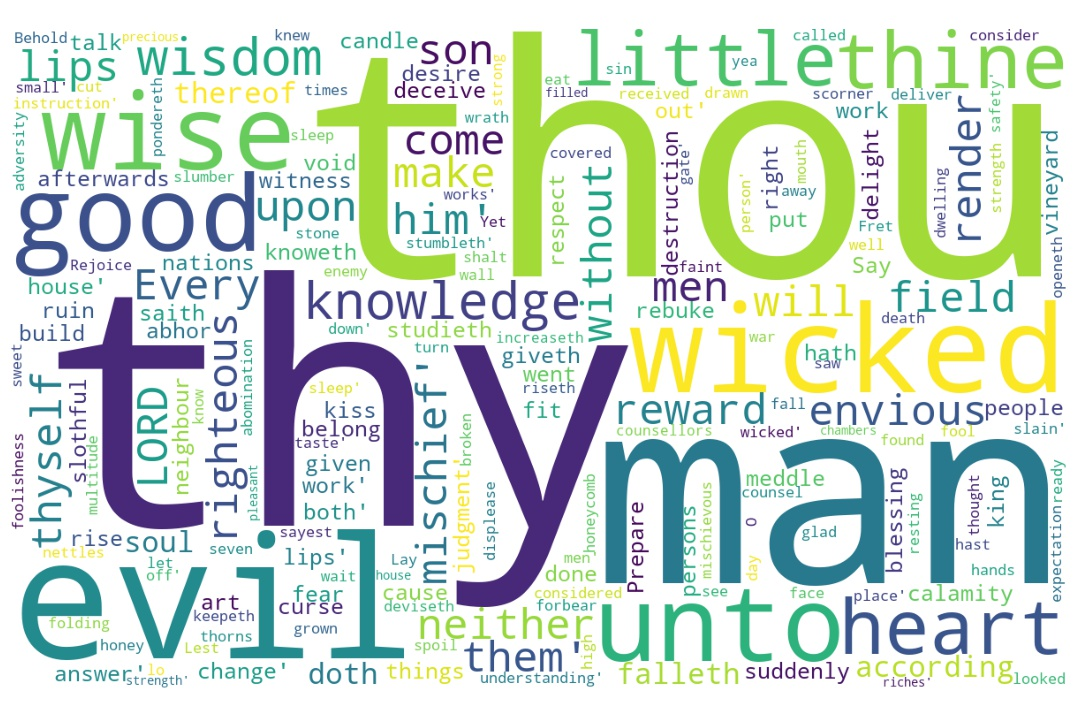
\includegraphics[width=\linewidth]{20OT-Proverbs/Proverb24-WordCloud.jpg}
  \caption{Proverb 24 Word Cloud}
  \label{fig:Proverb 24 word Cloud}
\end{figure}

\marginpar{\scriptsize \centering \fcolorbox{bone}{lime}{\textbf{HOUSE BUILT BY WISDOM}}\\ (Proverb 24:1-5) \begin{compactenum}[I.][8]
    \item \textbf{It is Put Up (Built)} \index[scripture]{Proverbs!Pro 24:03} (Pro 24:3)
    \item \textbf{It is Provided For} \index[scripture]{Proverbs!Pro 24:04} (Pro 24:4)
    \item \textbf{It has Precious Riches} \index[scripture]{Proverbs!Pro 24:04} (Pro 24:4)
    \item \textbf{It is Pleasant} \index[scripture]{Proverbs!Pro 24:04} (Pro 24:4)
    \item \textbf{It is Plenteous} \index[scripture]{Proverbs!Pro 24:04} (Pro 24:4)
    \item \textbf{It is Replete with Goods} \index[scripture]{Proverbs!Pro 24:04} (Pro 24:4)
    \item \textbf{It is Permanent} \index[scripture]{Proverbs!Pro 24:05} (Pro 24:5)
\end{compactenum}}

% \marginpar{\scriptsize \centering \fcolorbox{bone}{yellow}{\textbf{\textcolor[rgb]{1.00,1.00,1.00}{VOID OF UNDERSTANDING}}}\\ (Proverbs 24:1-5) \begin{compactenum}[I.][8]
\marginpar{\scriptsize \centering \fcolorbox{bone}{yellow}{\textbf{VOID OF UNDERSTANDING}}\\ (Proverb 24:1-5) \begin{compactenum}[I.][8]
    \item \textcolor[rgb]{0.00,0.00,0.00}{Is \textbf{Sensual} (\index[scripture]{Proverbs!Pro 7:7}Pro 7:7)}
    \item \textcolor[rgb]{0.00,0.00,0.00}{Reckless \textbf{Speech} (\index[scripture]{Proverbs!Pro 10:13}Pro 10:13)}
    \item \textcolor[rgb]{0.00,0.00,0.00}{Has \textbf{Schemes} (\index[scripture]{Proverbs!Pro 12:11}Pro 12:11)}
    \item \textcolor[rgb]{0.00,0.00,0.00}{Is \textbf{Surety} for Others (\index[scripture]{Proverbs!Pro 17:18}Pro 17:18)}
    \item \textcolor[rgb]{0.00,0.00,0.00}{Is \textbf{Slothful} (\index[scripture]{Proverbs!Pro 24:30}Pro 24:30)}\end{compactenum}}

\marginpar{\scriptsize \centering \fcolorbox{black}{black}{\textbf{\textcolor[rgb]{1.00,1.00,1.00}{THINGS OF THE SLOTHFUL}}}\\ (Proverbs 24:31-33) \begin{compactenum}[I.][8]
    \item \textcolor[rgb]{0.00,0.00,0.00}{His \textbf{Lands} (\index[scripture]{Proverbs!Pro 24:31}Pro 24:31)}
    \item \textcolor[rgb]{0.00,0.00,0.00}{His \textbf{Life} (\index[scripture]{Proverbs!Pro 24:31}Pro 24:31)}
    \item \textcolor[rgb]{0.00,0.00,0.00}{His \textbf{Loves} (\index[scripture]{Proverbs!Pro 24:31}Pro 24:31)}
    \item \textcolor[rgb]{0.00,0.00,0.00}{His \textbf{Learning} (\index[scripture]{Proverbs!Pro 24:31}Pro 24:31)}
    \item \textcolor[rgb]{0.00,0.00,0.00}{His \textbf{Longings} (\index[scripture]{Proverbs!Pro 24:31}Pro 24:31)}
\end{compactenum}}

\marginpar{\scriptsize \centering \fcolorbox{bone}{blue}{\textbf{\textcolor[rgb]{1.00,1.00,1.00}{FIVE JUST MEN}}}\\ (Proverbs 24:16)\\
%\textbf{Introduction:} There are ten references to ``just men'' in scripture. Proverb 9:9 tells us that a just man will listen to instruction and become wiser. Proverb 20:7 tells us that he will maintain integrity. Proverb 24:16 says that, when  he falls, he will get up and get back on the correct path.  Ecclesiastes 7:20 says that just men are difficult to find. Ecclesiastes 7:15 that a just man will go to his grace having nothing but integrity, while a wicked man prolongs his life.
\begin{compactenum}[I.][8]
    \item \textbf{Noah} \index[scripture]{Genesis!Gen 06:09} (Gen 6:9)
    \item \textbf{Joseph} \index[scripture]{Matthew!Mat 01:19} (Mat 1:19)
    \item \textbf{Jesus} \index[scripture]{Matthew!Mat 27:19} (Mat 27:19)
    \item \textbf{John} \index[scripture]{Mark!Mk 06:20} (Mk 6:20)
    \item \textbf{Cornelius} \index[scripture]{Acts!Acts 10:22} (Acts 10:22)
\end{compactenum}}

\footnote{\textcolor[cmyk]{0.99998,1,0,0}{\hyperlink{TOC}{Return to end of Table of Contents.}}}\footnote{\href{https://audiobible.com/bible/proverbs_24.htm}{\textcolor[cmyk]{0.99998,1,0,0}{Proverbs Audio}}}\textcolor[cmyk]{0.99998,1,0,0}{Be not thou envious against evil men, neither desire to be with them.}
[2] \textcolor[cmyk]{0.99998,1,0,0}{For their heart studieth destruction, and their lips talk of mischief.}\footnote{\textbf{Proverbs 15:28} - The heart of the righteous studieth to answer: but the mouth of the wicked poureth out evil things.}
[3] \textcolor[cmyk]{0.99998,1,0,0}{Through wisdom is an house \fcolorbox{bone}{lime}{builded}; and by \fcolorbox{bone}{MYGOLD}{understanding} it is established:}
[4] \textcolor[cmyk]{0.99998,1,0,0}{And by knowledge shall the chambers be \fcolorbox{bone}{lime}{filled} with all \fcolorbox{bone}{lime}{precious} and \fcolorbox{bone}{lime}{pleasant} riches.}
[5] \textcolor[cmyk]{0.99998,1,0,0}{A wise man \emph{is} strong; yea, a man of knowledge \fcolorbox{bone}{lime}{increaseth} strength.}
[6] \textcolor[cmyk]{0.99998,1,0,0}{For by wise counsel thou shalt make thy war: and in multitude of counsellors \emph{there} \emph{is} safety.}
[7] \textcolor[cmyk]{0.99998,1,0,0}{Wisdom \emph{is} too high for a fool: he openeth not his mouth in the gate.}
[8] \textcolor[cmyk]{0.99998,1,0,0}{He that deviseth to do evil shall be called a mischievous person.}\footnote{The connection of the word mischievous is clearly set in scripture in that it is used 5 times, in (1) Psalm 21:11, (2) Psalm 38:12, (3) Proverbs 24:8, (4) Ecclesiastes 10:13, and (5) Micah 7:3. Scripture sets the tone of mischievous as wicked and evil and not ``cute'' as used in the modern context. See, further, the use of the word ``mischief'' as above in verse 2. The word is perhaps best defined by its last use in Acts 13:10: And said, O full of all subtilty and all mischief, thou child of the devil, thou enemy of all righteousness, wilt thou not cease to pervert the right ways of the Lord?}
[9] \textcolor[cmyk]{0.99998,1,0,0}{The thought of foolishness \emph{is} sin: and the scorner \emph{is} an abomination to men.}
[10] \textcolor[cmyk]{0.99998,1,0,0}{\emph{If} thou faint in the day of adversity, thy strength \emph{is} small.}
[11] \textcolor[cmyk]{0.99998,1,0,0}{If thou forbear to deliver \emph{them} \emph{that} \emph{are} drawn unto death, and \emph{those} \emph{that} \emph{are} ready to be slain;}
[12] \textcolor[cmyk]{0.99998,1,0,0}{If thou sayest, Behold, we knew it not; doth not he that pondereth the heart consider \emph{it}? and he that keepeth thy soul, doth \emph{not} he know \emph{it}? and shall \emph{not} he render to \emph{every} man according to his works?}\footnote{\textbf{Jeremiah 17:9, 10} - he heart is deceitful above all things, and desperately wicked: who can know it? [10] I the LORD search the heart, I try the reins, even to give every man according to his ways, and according to the fruit of his doings. }\footnote{\textbf{Matthew 16:27} - For the Son of man shall come in the glory of his Father with his angels; and then he shall reward every man according to his works.}\footnote{\textbf{1 Timothy 4:14} - Alexander the coppersmith did me much evil: the Lord reward him according to his works:}\footnote{\textbf{Hebrews 4:12} - For the word of God is quick, and powerful, and sharper than any twoedged sword, piercing even to the dividing asunder of soul and spirit, and of the joints and marrow, and is a discerner of the thoughts and intents of the heart.}
[13] \textcolor[cmyk]{0.99998,1,0,0}{My son, eat thou honey, because \emph{it} \emph{is} good; and the honeycomb, \emph{which} \emph{is} sweet to thy taste:}
[14] \textcolor[cmyk]{0.99998,1,0,0}{So \emph{shall} the knowledge of wisdom \emph{be} unto thy soul: when thou hast found \emph{it}, then there shall be a reward, and thy expectation shall not be cut off.}
[15] \textcolor[cmyk]{0.99998,1,0,0}{Lay not wait, O wicked \emph{man}, against the dwelling of the righteous; spoil not his resting place:}
[16] \textcolor[cmyk]{0.99998,1,0,0}{For a just \emph{man} falleth seven times, and riseth up again: but the wicked shall fall into mischief.}
[17] \textcolor[cmyk]{0.99998,1,0,0}{Rejoice not when thine enemy falleth, and let not thine heart be glad when he stumbleth:}
[18] \textcolor[cmyk]{0.99998,1,0,0}{Lest the LORD see \emph{it}, and it displease him, and he turn away his wrath from him.}
[19] \textcolor[cmyk]{0.99998,1,0,0}{Fret not thyself because of evil \emph{men}, neither be thou envious at the wicked;}
[20] \textcolor[cmyk]{0.99998,1,0,0}{For there shall be no reward to the evil \emph{man}; the candle of the wicked shall be put out.}\footnote{\textbf{Job 21:17} - How oft is the candle of the wicked put out! and how oft cometh their destruction upon them! God distributeth sorrows in his anger.} 
[21] \textcolor[cmyk]{0.99998,1,0,0}{My son, fear thou the LORD and the king: \emph{and} meddle not with them that are given to change:}\footnote{\textbf{Daniel 7:25} - And he shall speak great words against the most High, and shall wear out the saints of the most High, and think to change times and laws: and they shall be given into his hand until a time and times and the dividing of time.}\footnote{\textbf{Malachi 3:6} - For I am the LORD, I change not; therefore ye sons of Jacob are not consumed.}
[22] \textcolor[cmyk]{0.99998,1,0,0}{For their calamity shall rise suddenly; and who knoweth the ruin of them both?}\footnote{\textbf{Obadiah 1:13} - Thou shouldest not have entered into the gate of my people in the day of their calamity; yea, thou shouldest not have looked on their affliction in the day of their calamity, nor have laid hands on their substance in the day of their calamity;}
[23] \textcolor[cmyk]{0.99998,1,0,0}{These \emph{things} also \emph{belong} to the wise. \emph{It} \emph{is} not good to have respect of persons in judgment.}\footnote{\textbf{2 Chronicles 19:7} - Wherefore now let the fear of the LORD be upon you; take heed and do it: for there is no iniquity with the LORD our God, nor respect of persons, nor taking of gifts.}\footnote{\textbf{Romans 2:11} - For there is no respect of persons with God.}\footnote{\textbf{Ephesians 6:9} - And, ye masters, do the same things unto them, forbearing threatening: knowing that your Master also is in heaven; neither is there respect of persons with him.}
[24] \textcolor[cmyk]{0.99998,1,0,0}{He that saith unto the wicked, Thou \emph{art} righteous; him shall the people curse, nations shall abhor him:}\footnote{\textbf{Romans 12:9} - Let love be without dissimulation. Abhor that which is evil; cleave to that which is good.}
[25] \textcolor[cmyk]{0.99998,1,0,0}{But to them that rebuke \emph{him} shall be delight, and a good blessing shall come upon them.}
[26] \textcolor[cmyk]{0.99998,1,0,0}{\emph{Every} \emph{man} shall kiss \emph{his} lips that giveth a right answer.}
[27] \textcolor[cmyk]{0.99998,1,0,0}{Prepare thy work without, and make it fit for thyself in the field; and afterwards build thine house.}
[28] \textcolor[cmyk]{0.99998,1,0,0}{Be not a witness against thy neighbour without cause; and deceive \emph{not} with thy lips.}
[29] \textcolor[cmyk]{0.99998,1,0,0}{Say not, I will do so to him as he hath done to me: I will render to the man according to his work.}
[30] \textcolor[cmyk]{0.99998,1,0,0}{I went by the field of the slothful, and by the vineyard of the man void of \fcolorbox{bone}{MYGOLD}{understanding};}
[31] \textcolor[cmyk]{0.99998,1,0,0}{And, lo, it was all grown over with thorns, \emph{and} nettles had covered the face thereof, and the stone wall thereof was broken down.}\footnote{\textbf{Job 30:7} - Among the bushes they brayed; under the nettles they were gathered together.}\footnote{\textbf{Isaiah 34:13} - And thorns shall come up in her palaces, nettles and brambles in the fortresses thereof: and it shall be an habitation of dragons, and a court for owls.}\footnote{\textbf{Hosea 9:6} - For, lo, they are gone because of destruction: Egypt shall gather them up, Memphis shall bury them: the pleasant places for their silver, nettles shall possess them: thorns shall be in their tabernacles.}\footnote{\textbf{Zephaniah 2:9} - Therefore as I live, saith the LORD of hosts, the God of Israel, Surely Moab shall be as Sodom, and the children of Ammon as Gomorrah, even the breeding of nettles, and saltpits, and a perpetual desolation: the residue of my people shall spoil them, and the remnant of my people shall possess them. }
[32] \textcolor[cmyk]{0.99998,1,0,0}{Then I saw, \emph{and} considered \emph{it} well: I looked upon \emph{it,} \emph{and} received instruction.}
[33] \textcolor[cmyk]{0.99998,1,0,0}{\emph{Yet} a little sleep, a little slumber, a little folding of the hands to sleep:}
[34] \textcolor[cmyk]{0.99998,1,0,0}{So shall thy poverty come \emph{as} one that travelleth; and thy want as an armed man.}




\index[NWIV]{13!Proverbs!Pro 24:1}\index[AWIP]{Be!Proverbs!Pro 24:1}\index[AWIP]{not!Proverbs!Pro 24:1}\index[AWIP]{thou!Proverbs!Pro 24:1}\index[AWIP]{envious!Proverbs!Pro 24:1}\index[AWIP]{against!Proverbs!Pro 24:1}\index[AWIP]{evil!Proverbs!Pro 24:1}\index[AWIP]{men!Proverbs!Pro 24:1}\index[AWIP]{neither!Proverbs!Pro 24:1}\index[AWIP]{desire!Proverbs!Pro 24:1}\index[AWIP]{to!Proverbs!Pro 24:1}\index[AWIP]{be!Proverbs!Pro 24:1}\index[AWIP]{with!Proverbs!Pro 24:1}\index[AWIP]{them!Proverbs!Pro 24:1}

\index[NWIV]{11!Proverbs!Pro 24:2}\index[AWIP]{For!Proverbs!Pro 24:2}\index[AWIP]{their!Proverbs!Pro 24:2}\index[AWIP]{their!Proverbs!Pro 24:2 (2)}\index[AWIP]{heart!Proverbs!Pro 24:2}\index[AWIP]{studieth!Proverbs!Pro 24:2}\index[AWIP]{destruction!Proverbs!Pro 24:2}\index[AWIP]{and!Proverbs!Pro 24:2}\index[AWIP]{lips!Proverbs!Pro 24:2}\index[AWIP]{talk!Proverbs!Pro 24:2}\index[AWIP]{of!Proverbs!Pro 24:2}\index[AWIP]{mischief!Proverbs!Pro 24:2}

\index[NWIV]{12!Proverbs!Pro 24:3}\index[AWIP]{Through!Proverbs!Pro 24:3}\index[AWIP]{wisdom!Proverbs!Pro 24:3}\index[AWIP]{is!Proverbs!Pro 24:3}\index[AWIP]{is!Proverbs!Pro 24:3 (2)}\index[AWIP]{an!Proverbs!Pro 24:3}\index[AWIP]{house!Proverbs!Pro 24:3}\index[AWIP]{builded!Proverbs!Pro 24:3}\index[AWIP]{and!Proverbs!Pro 24:3}\index[AWIP]{by!Proverbs!Pro 24:3}\index[AWIP]{understanding!Proverbs!Pro 24:3}\index[AWIP]{it!Proverbs!Pro 24:3}\index[AWIP]{established!Proverbs!Pro 24:3}

\index[NWIV]{14!Proverbs!Pro 24:4}\index[AWIP]{And!Proverbs!Pro 24:4}\index[AWIP]{by!Proverbs!Pro 24:4}\index[AWIP]{knowledge!Proverbs!Pro 24:4}\index[AWIP]{shall!Proverbs!Pro 24:4}\index[AWIP]{the!Proverbs!Pro 24:4}\index[AWIP]{chambers!Proverbs!Pro 24:4}\index[AWIP]{be!Proverbs!Pro 24:4}\index[AWIP]{filled!Proverbs!Pro 24:4}\index[AWIP]{with!Proverbs!Pro 24:4}\index[AWIP]{all!Proverbs!Pro 24:4}\index[AWIP]{precious!Proverbs!Pro 24:4}\index[AWIP]{and!Proverbs!Pro 24:4}\index[AWIP]{pleasant!Proverbs!Pro 24:4}\index[AWIP]{riches!Proverbs!Pro 24:4}

\index[NWIV]{12!Proverbs!Pro 24:5}\index[AWIP]{A!Proverbs!Pro 24:5}\index[AWIP]{wise!Proverbs!Pro 24:5}\index[AWIP]{man!Proverbs!Pro 24:5}\index[AWIP]{man!Proverbs!Pro 24:5 (2)}\index[AWIP]{\emph{is}!Proverbs!Pro 24:5}\index[AWIP]{strong!Proverbs!Pro 24:5}\index[AWIP]{yea!Proverbs!Pro 24:5}\index[AWIP]{a!Proverbs!Pro 24:5}\index[AWIP]{of!Proverbs!Pro 24:5}\index[AWIP]{knowledge!Proverbs!Pro 24:5}\index[AWIP]{increaseth!Proverbs!Pro 24:5}\index[AWIP]{strength!Proverbs!Pro 24:5}\index[AWIP]{\emph{is}!Proverbs!Pro 24:5}

\index[NWIV]{17!Proverbs!Pro 24:6}\index[AWIP]{For!Proverbs!Pro 24:6}\index[AWIP]{by!Proverbs!Pro 24:6}\index[AWIP]{wise!Proverbs!Pro 24:6}\index[AWIP]{counsel!Proverbs!Pro 24:6}\index[AWIP]{thou!Proverbs!Pro 24:6}\index[AWIP]{shalt!Proverbs!Pro 24:6}\index[AWIP]{make!Proverbs!Pro 24:6}\index[AWIP]{thy!Proverbs!Pro 24:6}\index[AWIP]{war!Proverbs!Pro 24:6}\index[AWIP]{and!Proverbs!Pro 24:6}\index[AWIP]{in!Proverbs!Pro 24:6}\index[AWIP]{multitude!Proverbs!Pro 24:6}\index[AWIP]{of!Proverbs!Pro 24:6}\index[AWIP]{counsellors!Proverbs!Pro 24:6}\index[AWIP]{\emph{there}!Proverbs!Pro 24:6}\index[AWIP]{\emph{is}!Proverbs!Pro 24:6}\index[AWIP]{safety!Proverbs!Pro 24:6}\index[AWIP]{\emph{there}!Proverbs!Pro 24:6}\index[AWIP]{\emph{is}!Proverbs!Pro 24:6}

\index[NWIV]{15!Proverbs!Pro 24:7}\index[AWIP]{Wisdom!Proverbs!Pro 24:7}\index[AWIP]{\emph{is}!Proverbs!Pro 24:7}\index[AWIP]{too!Proverbs!Pro 24:7}\index[AWIP]{high!Proverbs!Pro 24:7}\index[AWIP]{for!Proverbs!Pro 24:7}\index[AWIP]{a!Proverbs!Pro 24:7}\index[AWIP]{fool!Proverbs!Pro 24:7}\index[AWIP]{he!Proverbs!Pro 24:7}\index[AWIP]{openeth!Proverbs!Pro 24:7}\index[AWIP]{not!Proverbs!Pro 24:7}\index[AWIP]{his!Proverbs!Pro 24:7}\index[AWIP]{mouth!Proverbs!Pro 24:7}\index[AWIP]{in!Proverbs!Pro 24:7}\index[AWIP]{the!Proverbs!Pro 24:7}\index[AWIP]{gate!Proverbs!Pro 24:7}\index[AWIP]{\emph{is}!Proverbs!Pro 24:7}

\index[NWIV]{12!Proverbs!Pro 24:8}\index[AWIP]{He!Proverbs!Pro 24:8}\index[AWIP]{that!Proverbs!Pro 24:8}\index[AWIP]{deviseth!Proverbs!Pro 24:8}\index[AWIP]{to!Proverbs!Pro 24:8}\index[AWIP]{do!Proverbs!Pro 24:8}\index[AWIP]{evil!Proverbs!Pro 24:8}\index[AWIP]{shall!Proverbs!Pro 24:8}\index[AWIP]{be!Proverbs!Pro 24:8}\index[AWIP]{called!Proverbs!Pro 24:8}\index[AWIP]{a!Proverbs!Pro 24:8}\index[AWIP]{mischievous!Proverbs!Pro 24:8}\index[AWIP]{person!Proverbs!Pro 24:8}

\index[NWIV]{14!Proverbs!Pro 24:9}\index[AWIP]{The!Proverbs!Pro 24:9}\index[AWIP]{thought!Proverbs!Pro 24:9}\index[AWIP]{of!Proverbs!Pro 24:9}\index[AWIP]{foolishness!Proverbs!Pro 24:9}\index[AWIP]{\emph{is}!Proverbs!Pro 24:9}\index[AWIP]{\emph{is}!Proverbs!Pro 24:9 (2)}\index[AWIP]{sin!Proverbs!Pro 24:9}\index[AWIP]{and!Proverbs!Pro 24:9}\index[AWIP]{the!Proverbs!Pro 24:9}\index[AWIP]{scorner!Proverbs!Pro 24:9}\index[AWIP]{an!Proverbs!Pro 24:9}\index[AWIP]{abomination!Proverbs!Pro 24:9}\index[AWIP]{to!Proverbs!Pro 24:9}\index[AWIP]{men!Proverbs!Pro 24:9}\index[AWIP]{\emph{is}!Proverbs!Pro 24:9}\index[AWIP]{\emph{is}!Proverbs!Pro 24:9 (2)}

\index[NWIV]{12!Proverbs!Pro 24:10}\index[AWIP]{\emph{If}!Proverbs!Pro 24:10}\index[AWIP]{thou!Proverbs!Pro 24:10}\index[AWIP]{faint!Proverbs!Pro 24:10}\index[AWIP]{in!Proverbs!Pro 24:10}\index[AWIP]{the!Proverbs!Pro 24:10}\index[AWIP]{day!Proverbs!Pro 24:10}\index[AWIP]{of!Proverbs!Pro 24:10}\index[AWIP]{adversity!Proverbs!Pro 24:10}\index[AWIP]{thy!Proverbs!Pro 24:10}\index[AWIP]{strength!Proverbs!Pro 24:10}\index[AWIP]{\emph{is}!Proverbs!Pro 24:10}\index[AWIP]{small!Proverbs!Pro 24:10}\index[AWIP]{\emph{If}!Proverbs!Pro 24:10}\index[AWIP]{\emph{is}!Proverbs!Pro 24:10}

\index[NWIV]{19!Proverbs!Pro 24:11}\index[AWIP]{If!Proverbs!Pro 24:11}\index[AWIP]{thou!Proverbs!Pro 24:11}\index[AWIP]{forbear!Proverbs!Pro 24:11}\index[AWIP]{to!Proverbs!Pro 24:11}\index[AWIP]{to!Proverbs!Pro 24:11 (2)}\index[AWIP]{deliver!Proverbs!Pro 24:11}\index[AWIP]{\emph{them}!Proverbs!Pro 24:11}\index[AWIP]{\emph{that}!Proverbs!Pro 24:11}\index[AWIP]{\emph{that}!Proverbs!Pro 24:11 (2)}\index[AWIP]{\emph{are}!Proverbs!Pro 24:11}\index[AWIP]{\emph{are}!Proverbs!Pro 24:11 (2)}\index[AWIP]{drawn!Proverbs!Pro 24:11}\index[AWIP]{unto!Proverbs!Pro 24:11}\index[AWIP]{death!Proverbs!Pro 24:11}\index[AWIP]{and!Proverbs!Pro 24:11}\index[AWIP]{\emph{those}!Proverbs!Pro 24:11}\index[AWIP]{ready!Proverbs!Pro 24:11}\index[AWIP]{be!Proverbs!Pro 24:11}\index[AWIP]{slain!Proverbs!Pro 24:11}\index[AWIP]{\emph{them}!Proverbs!Pro 24:11}\index[AWIP]{\emph{that}!Proverbs!Pro 24:11}\index[AWIP]{\emph{that}!Proverbs!Pro 24:11 (2)}\index[AWIP]{\emph{are}!Proverbs!Pro 24:11}\index[AWIP]{\emph{are}!Proverbs!Pro 24:11 (2)}\index[AWIP]{\emph{those}!Proverbs!Pro 24:11}

\index[NWIV]{40!Proverbs!Pro 24:12}\index[AWIP]{If!Proverbs!Pro 24:12}\index[AWIP]{thou!Proverbs!Pro 24:12}\index[AWIP]{sayest!Proverbs!Pro 24:12}\index[AWIP]{Behold!Proverbs!Pro 24:12}\index[AWIP]{we!Proverbs!Pro 24:12}\index[AWIP]{knew!Proverbs!Pro 24:12}\index[AWIP]{it!Proverbs!Pro 24:12}\index[AWIP]{not!Proverbs!Pro 24:12}\index[AWIP]{not!Proverbs!Pro 24:12 (2)}\index[AWIP]{doth!Proverbs!Pro 24:12}\index[AWIP]{doth!Proverbs!Pro 24:12 (2)}\index[AWIP]{he!Proverbs!Pro 24:12}\index[AWIP]{he!Proverbs!Pro 24:12 (2)}\index[AWIP]{he!Proverbs!Pro 24:12 (3)}\index[AWIP]{he!Proverbs!Pro 24:12 (4)}\index[AWIP]{that!Proverbs!Pro 24:12}\index[AWIP]{that!Proverbs!Pro 24:12 (2)}\index[AWIP]{pondereth!Proverbs!Pro 24:12}\index[AWIP]{the!Proverbs!Pro 24:12}\index[AWIP]{heart!Proverbs!Pro 24:12}\index[AWIP]{consider!Proverbs!Pro 24:12}\index[AWIP]{\emph{it}?!Proverbs!Pro 24:12}\index[AWIP]{\emph{it}?!Proverbs!Pro 24:12 (2)}\index[AWIP]{and!Proverbs!Pro 24:12}\index[AWIP]{and!Proverbs!Pro 24:12 (2)}\index[AWIP]{keepeth!Proverbs!Pro 24:12}\index[AWIP]{thy!Proverbs!Pro 24:12}\index[AWIP]{soul!Proverbs!Pro 24:12}\index[AWIP]{\emph{not}!Proverbs!Pro 24:12}\index[AWIP]{\emph{not}!Proverbs!Pro 24:12 (2)}\index[AWIP]{know!Proverbs!Pro 24:12}\index[AWIP]{shall!Proverbs!Pro 24:12}\index[AWIP]{render!Proverbs!Pro 24:12}\index[AWIP]{to!Proverbs!Pro 24:12}\index[AWIP]{to!Proverbs!Pro 24:12 (2)}\index[AWIP]{\emph{every}!Proverbs!Pro 24:12}\index[AWIP]{man!Proverbs!Pro 24:12}\index[AWIP]{according!Proverbs!Pro 24:12}\index[AWIP]{his!Proverbs!Pro 24:12}\index[AWIP]{works?!Proverbs!Pro 24:12}\index[AWIP]{\emph{it}?!Proverbs!Pro 24:12}\index[AWIP]{\emph{it}?!Proverbs!Pro 24:12 (2)}\index[AWIP]{\emph{not}!Proverbs!Pro 24:12}\index[AWIP]{\emph{not}!Proverbs!Pro 24:12 (2)}\index[AWIP]{\emph{every}!Proverbs!Pro 24:12}

\index[NWIV]{18!Proverbs!Pro 24:13}\index[AWIP]{My!Proverbs!Pro 24:13}\index[AWIP]{son!Proverbs!Pro 24:13}\index[AWIP]{eat!Proverbs!Pro 24:13}\index[AWIP]{thou!Proverbs!Pro 24:13}\index[AWIP]{honey!Proverbs!Pro 24:13}\index[AWIP]{because!Proverbs!Pro 24:13}\index[AWIP]{\emph{it}!Proverbs!Pro 24:13}\index[AWIP]{\emph{is}!Proverbs!Pro 24:13}\index[AWIP]{\emph{is}!Proverbs!Pro 24:13 (2)}\index[AWIP]{good!Proverbs!Pro 24:13}\index[AWIP]{and!Proverbs!Pro 24:13}\index[AWIP]{the!Proverbs!Pro 24:13}\index[AWIP]{honeycomb!Proverbs!Pro 24:13}\index[AWIP]{\emph{which}!Proverbs!Pro 24:13}\index[AWIP]{sweet!Proverbs!Pro 24:13}\index[AWIP]{to!Proverbs!Pro 24:13}\index[AWIP]{thy!Proverbs!Pro 24:13}\index[AWIP]{taste!Proverbs!Pro 24:13}\index[AWIP]{\emph{it}!Proverbs!Pro 24:13}\index[AWIP]{\emph{is}!Proverbs!Pro 24:13}\index[AWIP]{\emph{is}!Proverbs!Pro 24:13 (2)}\index[AWIP]{\emph{which}!Proverbs!Pro 24:13}

\index[NWIV]{29!Proverbs!Pro 24:14}\index[AWIP]{So!Proverbs!Pro 24:14}\index[AWIP]{\emph{shall}!Proverbs!Pro 24:14}\index[AWIP]{the!Proverbs!Pro 24:14}\index[AWIP]{knowledge!Proverbs!Pro 24:14}\index[AWIP]{of!Proverbs!Pro 24:14}\index[AWIP]{wisdom!Proverbs!Pro 24:14}\index[AWIP]{\emph{be}!Proverbs!Pro 24:14}\index[AWIP]{unto!Proverbs!Pro 24:14}\index[AWIP]{thy!Proverbs!Pro 24:14}\index[AWIP]{thy!Proverbs!Pro 24:14 (2)}\index[AWIP]{soul!Proverbs!Pro 24:14}\index[AWIP]{when!Proverbs!Pro 24:14}\index[AWIP]{thou!Proverbs!Pro 24:14}\index[AWIP]{hast!Proverbs!Pro 24:14}\index[AWIP]{found!Proverbs!Pro 24:14}\index[AWIP]{\emph{it}!Proverbs!Pro 24:14}\index[AWIP]{then!Proverbs!Pro 24:14}\index[AWIP]{there!Proverbs!Pro 24:14}\index[AWIP]{shall!Proverbs!Pro 24:14}\index[AWIP]{shall!Proverbs!Pro 24:14 (2)}\index[AWIP]{be!Proverbs!Pro 24:14}\index[AWIP]{be!Proverbs!Pro 24:14 (2)}\index[AWIP]{a!Proverbs!Pro 24:14}\index[AWIP]{reward!Proverbs!Pro 24:14}\index[AWIP]{and!Proverbs!Pro 24:14}\index[AWIP]{expectation!Proverbs!Pro 24:14}\index[AWIP]{not!Proverbs!Pro 24:14}\index[AWIP]{cut!Proverbs!Pro 24:14}\index[AWIP]{off!Proverbs!Pro 24:14}\index[AWIP]{\emph{shall}!Proverbs!Pro 24:14}\index[AWIP]{\emph{be}!Proverbs!Pro 24:14}\index[AWIP]{\emph{it}!Proverbs!Pro 24:14}

\index[NWIV]{17!Proverbs!Pro 24:15}\index[AWIP]{Lay!Proverbs!Pro 24:15}\index[AWIP]{not!Proverbs!Pro 24:15}\index[AWIP]{not!Proverbs!Pro 24:15 (2)}\index[AWIP]{wait!Proverbs!Pro 24:15}\index[AWIP]{O!Proverbs!Pro 24:15}\index[AWIP]{wicked!Proverbs!Pro 24:15}\index[AWIP]{\emph{man}!Proverbs!Pro 24:15}\index[AWIP]{against!Proverbs!Pro 24:15}\index[AWIP]{the!Proverbs!Pro 24:15}\index[AWIP]{the!Proverbs!Pro 24:15 (2)}\index[AWIP]{dwelling!Proverbs!Pro 24:15}\index[AWIP]{of!Proverbs!Pro 24:15}\index[AWIP]{righteous!Proverbs!Pro 24:15}\index[AWIP]{spoil!Proverbs!Pro 24:15}\index[AWIP]{his!Proverbs!Pro 24:15}\index[AWIP]{resting!Proverbs!Pro 24:15}\index[AWIP]{place!Proverbs!Pro 24:15}\index[AWIP]{\emph{man}!Proverbs!Pro 24:15}

\index[NWIV]{18!Proverbs!Pro 24:16}\index[AWIP]{For!Proverbs!Pro 24:16}\index[AWIP]{a!Proverbs!Pro 24:16}\index[AWIP]{just!Proverbs!Pro 24:16}\index[AWIP]{\emph{man}!Proverbs!Pro 24:16}\index[AWIP]{falleth!Proverbs!Pro 24:16}\index[AWIP]{seven!Proverbs!Pro 24:16}\index[AWIP]{times!Proverbs!Pro 24:16}\index[AWIP]{and!Proverbs!Pro 24:16}\index[AWIP]{riseth!Proverbs!Pro 24:16}\index[AWIP]{up!Proverbs!Pro 24:16}\index[AWIP]{again!Proverbs!Pro 24:16}\index[AWIP]{but!Proverbs!Pro 24:16}\index[AWIP]{the!Proverbs!Pro 24:16}\index[AWIP]{wicked!Proverbs!Pro 24:16}\index[AWIP]{shall!Proverbs!Pro 24:16}\index[AWIP]{fall!Proverbs!Pro 24:16}\index[AWIP]{into!Proverbs!Pro 24:16}\index[AWIP]{mischief!Proverbs!Pro 24:16}\index[AWIP]{\emph{man}!Proverbs!Pro 24:16}

\index[NWIV]{16!Proverbs!Pro 24:17}\index[AWIP]{Rejoice!Proverbs!Pro 24:17}\index[AWIP]{not!Proverbs!Pro 24:17}\index[AWIP]{not!Proverbs!Pro 24:17 (2)}\index[AWIP]{when!Proverbs!Pro 24:17}\index[AWIP]{when!Proverbs!Pro 24:17 (2)}\index[AWIP]{thine!Proverbs!Pro 24:17}\index[AWIP]{thine!Proverbs!Pro 24:17 (2)}\index[AWIP]{enemy!Proverbs!Pro 24:17}\index[AWIP]{falleth!Proverbs!Pro 24:17}\index[AWIP]{and!Proverbs!Pro 24:17}\index[AWIP]{let!Proverbs!Pro 24:17}\index[AWIP]{heart!Proverbs!Pro 24:17}\index[AWIP]{be!Proverbs!Pro 24:17}\index[AWIP]{glad!Proverbs!Pro 24:17}\index[AWIP]{he!Proverbs!Pro 24:17}\index[AWIP]{stumbleth!Proverbs!Pro 24:17}

\index[NWIV]{17!Proverbs!Pro 24:18}\index[AWIP]{Lest!Proverbs!Pro 24:18}\index[AWIP]{the!Proverbs!Pro 24:18}\index[AWIP]{LORD!Proverbs!Pro 24:18}\index[AWIP]{see!Proverbs!Pro 24:18}\index[AWIP]{\emph{it}!Proverbs!Pro 24:18}\index[AWIP]{and!Proverbs!Pro 24:18}\index[AWIP]{and!Proverbs!Pro 24:18 (2)}\index[AWIP]{it!Proverbs!Pro 24:18}\index[AWIP]{displease!Proverbs!Pro 24:18}\index[AWIP]{him!Proverbs!Pro 24:18}\index[AWIP]{him!Proverbs!Pro 24:18 (2)}\index[AWIP]{he!Proverbs!Pro 24:18}\index[AWIP]{turn!Proverbs!Pro 24:18}\index[AWIP]{away!Proverbs!Pro 24:18}\index[AWIP]{his!Proverbs!Pro 24:18}\index[AWIP]{wrath!Proverbs!Pro 24:18}\index[AWIP]{from!Proverbs!Pro 24:18}\index[AWIP]{\emph{it}!Proverbs!Pro 24:18}

\index[NWIV]{14!Proverbs!Pro 24:19}\index[AWIP]{Fret!Proverbs!Pro 24:19}\index[AWIP]{not!Proverbs!Pro 24:19}\index[AWIP]{thyself!Proverbs!Pro 24:19}\index[AWIP]{because!Proverbs!Pro 24:19}\index[AWIP]{of!Proverbs!Pro 24:19}\index[AWIP]{evil!Proverbs!Pro 24:19}\index[AWIP]{\emph{men}!Proverbs!Pro 24:19}\index[AWIP]{neither!Proverbs!Pro 24:19}\index[AWIP]{be!Proverbs!Pro 24:19}\index[AWIP]{thou!Proverbs!Pro 24:19}\index[AWIP]{envious!Proverbs!Pro 24:19}\index[AWIP]{at!Proverbs!Pro 24:19}\index[AWIP]{the!Proverbs!Pro 24:19}\index[AWIP]{wicked!Proverbs!Pro 24:19}\index[AWIP]{\emph{men}!Proverbs!Pro 24:19}

\index[NWIV]{19!Proverbs!Pro 24:20}\index[AWIP]{For!Proverbs!Pro 24:20}\index[AWIP]{there!Proverbs!Pro 24:20}\index[AWIP]{shall!Proverbs!Pro 24:20}\index[AWIP]{shall!Proverbs!Pro 24:20 (2)}\index[AWIP]{be!Proverbs!Pro 24:20}\index[AWIP]{be!Proverbs!Pro 24:20 (2)}\index[AWIP]{no!Proverbs!Pro 24:20}\index[AWIP]{reward!Proverbs!Pro 24:20}\index[AWIP]{to!Proverbs!Pro 24:20}\index[AWIP]{the!Proverbs!Pro 24:20}\index[AWIP]{the!Proverbs!Pro 24:20 (2)}\index[AWIP]{the!Proverbs!Pro 24:20 (3)}\index[AWIP]{evil!Proverbs!Pro 24:20}\index[AWIP]{\emph{man}!Proverbs!Pro 24:20}\index[AWIP]{candle!Proverbs!Pro 24:20}\index[AWIP]{of!Proverbs!Pro 24:20}\index[AWIP]{wicked!Proverbs!Pro 24:20}\index[AWIP]{put!Proverbs!Pro 24:20}\index[AWIP]{out!Proverbs!Pro 24:20}\index[AWIP]{\emph{man}!Proverbs!Pro 24:20}

\index[NWIV]{19!Proverbs!Pro 24:21}\index[AWIP]{My!Proverbs!Pro 24:21}\index[AWIP]{son!Proverbs!Pro 24:21}\index[AWIP]{fear!Proverbs!Pro 24:21}\index[AWIP]{thou!Proverbs!Pro 24:21}\index[AWIP]{the!Proverbs!Pro 24:21}\index[AWIP]{the!Proverbs!Pro 24:21 (2)}\index[AWIP]{LORD!Proverbs!Pro 24:21}\index[AWIP]{and!Proverbs!Pro 24:21}\index[AWIP]{king!Proverbs!Pro 24:21}\index[AWIP]{\emph{and}!Proverbs!Pro 24:21}\index[AWIP]{meddle!Proverbs!Pro 24:21}\index[AWIP]{not!Proverbs!Pro 24:21}\index[AWIP]{with!Proverbs!Pro 24:21}\index[AWIP]{them!Proverbs!Pro 24:21}\index[AWIP]{that!Proverbs!Pro 24:21}\index[AWIP]{are!Proverbs!Pro 24:21}\index[AWIP]{given!Proverbs!Pro 24:21}\index[AWIP]{to!Proverbs!Pro 24:21}\index[AWIP]{change!Proverbs!Pro 24:21}\index[AWIP]{\emph{and}!Proverbs!Pro 24:21}

\index[NWIV]{14!Proverbs!Pro 24:22}\index[AWIP]{For!Proverbs!Pro 24:22}\index[AWIP]{their!Proverbs!Pro 24:22}\index[AWIP]{calamity!Proverbs!Pro 24:22}\index[AWIP]{shall!Proverbs!Pro 24:22}\index[AWIP]{rise!Proverbs!Pro 24:22}\index[AWIP]{suddenly!Proverbs!Pro 24:22}\index[AWIP]{and!Proverbs!Pro 24:22}\index[AWIP]{who!Proverbs!Pro 24:22}\index[AWIP]{knoweth!Proverbs!Pro 24:22}\index[AWIP]{the!Proverbs!Pro 24:22}\index[AWIP]{ruin!Proverbs!Pro 24:22}\index[AWIP]{of!Proverbs!Pro 24:22}\index[AWIP]{them!Proverbs!Pro 24:22}\index[AWIP]{both?!Proverbs!Pro 24:22}

\index[NWIV]{18!Proverbs!Pro 24:23}\index[AWIP]{These!Proverbs!Pro 24:23}\index[AWIP]{\emph{things}!Proverbs!Pro 24:23}\index[AWIP]{also!Proverbs!Pro 24:23}\index[AWIP]{\emph{belong}!Proverbs!Pro 24:23}\index[AWIP]{to!Proverbs!Pro 24:23}\index[AWIP]{to!Proverbs!Pro 24:23 (2)}\index[AWIP]{the!Proverbs!Pro 24:23}\index[AWIP]{wise!Proverbs!Pro 24:23}\index[AWIP]{\emph{It}!Proverbs!Pro 24:23}\index[AWIP]{\emph{is}!Proverbs!Pro 24:23}\index[AWIP]{not!Proverbs!Pro 24:23}\index[AWIP]{good!Proverbs!Pro 24:23}\index[AWIP]{have!Proverbs!Pro 24:23}\index[AWIP]{respect!Proverbs!Pro 24:23}\index[AWIP]{of!Proverbs!Pro 24:23}\index[AWIP]{persons!Proverbs!Pro 24:23}\index[AWIP]{in!Proverbs!Pro 24:23}\index[AWIP]{judgment!Proverbs!Pro 24:23}\index[AWIP]{\emph{things}!Proverbs!Pro 24:23}\index[AWIP]{\emph{belong}!Proverbs!Pro 24:23}\index[AWIP]{\emph{It}!Proverbs!Pro 24:23}\index[AWIP]{\emph{is}!Proverbs!Pro 24:23}

\index[NWIV]{18!Proverbs!Pro 24:24}\index[AWIP]{He!Proverbs!Pro 24:24}\index[AWIP]{that!Proverbs!Pro 24:24}\index[AWIP]{saith!Proverbs!Pro 24:24}\index[AWIP]{unto!Proverbs!Pro 24:24}\index[AWIP]{the!Proverbs!Pro 24:24}\index[AWIP]{the!Proverbs!Pro 24:24 (2)}\index[AWIP]{wicked!Proverbs!Pro 24:24}\index[AWIP]{Thou!Proverbs!Pro 24:24}\index[AWIP]{\emph{art}!Proverbs!Pro 24:24}\index[AWIP]{righteous!Proverbs!Pro 24:24}\index[AWIP]{him!Proverbs!Pro 24:24}\index[AWIP]{him!Proverbs!Pro 24:24 (2)}\index[AWIP]{shall!Proverbs!Pro 24:24}\index[AWIP]{shall!Proverbs!Pro 24:24 (2)}\index[AWIP]{people!Proverbs!Pro 24:24}\index[AWIP]{curse!Proverbs!Pro 24:24}\index[AWIP]{nations!Proverbs!Pro 24:24}\index[AWIP]{abhor!Proverbs!Pro 24:24}\index[AWIP]{\emph{art}!Proverbs!Pro 24:24}

\index[NWIV]{17!Proverbs!Pro 24:25}\index[AWIP]{But!Proverbs!Pro 24:25}\index[AWIP]{to!Proverbs!Pro 24:25}\index[AWIP]{them!Proverbs!Pro 24:25}\index[AWIP]{them!Proverbs!Pro 24:25 (2)}\index[AWIP]{that!Proverbs!Pro 24:25}\index[AWIP]{rebuke!Proverbs!Pro 24:25}\index[AWIP]{\emph{him}!Proverbs!Pro 24:25}\index[AWIP]{shall!Proverbs!Pro 24:25}\index[AWIP]{shall!Proverbs!Pro 24:25 (2)}\index[AWIP]{be!Proverbs!Pro 24:25}\index[AWIP]{delight!Proverbs!Pro 24:25}\index[AWIP]{and!Proverbs!Pro 24:25}\index[AWIP]{a!Proverbs!Pro 24:25}\index[AWIP]{good!Proverbs!Pro 24:25}\index[AWIP]{blessing!Proverbs!Pro 24:25}\index[AWIP]{come!Proverbs!Pro 24:25}\index[AWIP]{upon!Proverbs!Pro 24:25}\index[AWIP]{\emph{him}!Proverbs!Pro 24:25}

\index[NWIV]{11!Proverbs!Pro 24:26}\index[AWIP]{\emph{Every}!Proverbs!Pro 24:26}\index[AWIP]{\emph{man}!Proverbs!Pro 24:26}\index[AWIP]{shall!Proverbs!Pro 24:26}\index[AWIP]{kiss!Proverbs!Pro 24:26}\index[AWIP]{\emph{his}!Proverbs!Pro 24:26}\index[AWIP]{lips!Proverbs!Pro 24:26}\index[AWIP]{that!Proverbs!Pro 24:26}\index[AWIP]{giveth!Proverbs!Pro 24:26}\index[AWIP]{a!Proverbs!Pro 24:26}\index[AWIP]{right!Proverbs!Pro 24:26}\index[AWIP]{answer!Proverbs!Pro 24:26}\index[AWIP]{\emph{Every}!Proverbs!Pro 24:26}\index[AWIP]{\emph{man}!Proverbs!Pro 24:26}\index[AWIP]{\emph{his}!Proverbs!Pro 24:26}

\index[NWIV]{18!Proverbs!Pro 24:27}\index[AWIP]{Prepare!Proverbs!Pro 24:27}\index[AWIP]{thy!Proverbs!Pro 24:27}\index[AWIP]{work!Proverbs!Pro 24:27}\index[AWIP]{without!Proverbs!Pro 24:27}\index[AWIP]{and!Proverbs!Pro 24:27}\index[AWIP]{and!Proverbs!Pro 24:27 (2)}\index[AWIP]{make!Proverbs!Pro 24:27}\index[AWIP]{it!Proverbs!Pro 24:27}\index[AWIP]{fit!Proverbs!Pro 24:27}\index[AWIP]{for!Proverbs!Pro 24:27}\index[AWIP]{thyself!Proverbs!Pro 24:27}\index[AWIP]{in!Proverbs!Pro 24:27}\index[AWIP]{the!Proverbs!Pro 24:27}\index[AWIP]{field!Proverbs!Pro 24:27}\index[AWIP]{afterwards!Proverbs!Pro 24:27}\index[AWIP]{build!Proverbs!Pro 24:27}\index[AWIP]{thine!Proverbs!Pro 24:27}\index[AWIP]{house!Proverbs!Pro 24:27}

\index[NWIV]{15!Proverbs!Pro 24:28}\index[AWIP]{Be!Proverbs!Pro 24:28}\index[AWIP]{not!Proverbs!Pro 24:28}\index[AWIP]{a!Proverbs!Pro 24:28}\index[AWIP]{witness!Proverbs!Pro 24:28}\index[AWIP]{against!Proverbs!Pro 24:28}\index[AWIP]{thy!Proverbs!Pro 24:28}\index[AWIP]{thy!Proverbs!Pro 24:28 (2)}\index[AWIP]{neighbour!Proverbs!Pro 24:28}\index[AWIP]{without!Proverbs!Pro 24:28}\index[AWIP]{cause!Proverbs!Pro 24:28}\index[AWIP]{and!Proverbs!Pro 24:28}\index[AWIP]{deceive!Proverbs!Pro 24:28}\index[AWIP]{\emph{not}!Proverbs!Pro 24:28}\index[AWIP]{with!Proverbs!Pro 24:28}\index[AWIP]{lips!Proverbs!Pro 24:28}\index[AWIP]{\emph{not}!Proverbs!Pro 24:28}

\index[NWIV]{24!Proverbs!Pro 24:29}\index[AWIP]{Say!Proverbs!Pro 24:29}\index[AWIP]{not!Proverbs!Pro 24:29}\index[AWIP]{I!Proverbs!Pro 24:29}\index[AWIP]{I!Proverbs!Pro 24:29 (2)}\index[AWIP]{will!Proverbs!Pro 24:29}\index[AWIP]{will!Proverbs!Pro 24:29 (2)}\index[AWIP]{do!Proverbs!Pro 24:29}\index[AWIP]{so!Proverbs!Pro 24:29}\index[AWIP]{to!Proverbs!Pro 24:29}\index[AWIP]{to!Proverbs!Pro 24:29 (2)}\index[AWIP]{to!Proverbs!Pro 24:29 (3)}\index[AWIP]{to!Proverbs!Pro 24:29 (4)}\index[AWIP]{him!Proverbs!Pro 24:29}\index[AWIP]{as!Proverbs!Pro 24:29}\index[AWIP]{he!Proverbs!Pro 24:29}\index[AWIP]{hath!Proverbs!Pro 24:29}\index[AWIP]{done!Proverbs!Pro 24:29}\index[AWIP]{me!Proverbs!Pro 24:29}\index[AWIP]{render!Proverbs!Pro 24:29}\index[AWIP]{the!Proverbs!Pro 24:29}\index[AWIP]{man!Proverbs!Pro 24:29}\index[AWIP]{according!Proverbs!Pro 24:29}\index[AWIP]{his!Proverbs!Pro 24:29}\index[AWIP]{work!Proverbs!Pro 24:29}

\index[NWIV]{18!Proverbs!Pro 24:30}\index[AWIP]{I!Proverbs!Pro 24:30}\index[AWIP]{went!Proverbs!Pro 24:30}\index[AWIP]{by!Proverbs!Pro 24:30}\index[AWIP]{by!Proverbs!Pro 24:30 (2)}\index[AWIP]{the!Proverbs!Pro 24:30}\index[AWIP]{the!Proverbs!Pro 24:30 (2)}\index[AWIP]{the!Proverbs!Pro 24:30 (3)}\index[AWIP]{the!Proverbs!Pro 24:30 (4)}\index[AWIP]{field!Proverbs!Pro 24:30}\index[AWIP]{of!Proverbs!Pro 24:30}\index[AWIP]{of!Proverbs!Pro 24:30 (2)}\index[AWIP]{of!Proverbs!Pro 24:30 (3)}\index[AWIP]{slothful!Proverbs!Pro 24:30}\index[AWIP]{and!Proverbs!Pro 24:30}\index[AWIP]{vineyard!Proverbs!Pro 24:30}\index[AWIP]{man!Proverbs!Pro 24:30}\index[AWIP]{void!Proverbs!Pro 24:30}\index[AWIP]{understanding!Proverbs!Pro 24:30}

\index[NWIV]{24!Proverbs!Pro 24:31}\index[AWIP]{And!Proverbs!Pro 24:31}\index[AWIP]{lo!Proverbs!Pro 24:31}\index[AWIP]{it!Proverbs!Pro 24:31}\index[AWIP]{was!Proverbs!Pro 24:31}\index[AWIP]{was!Proverbs!Pro 24:31 (2)}\index[AWIP]{all!Proverbs!Pro 24:31}\index[AWIP]{grown!Proverbs!Pro 24:31}\index[AWIP]{over!Proverbs!Pro 24:31}\index[AWIP]{with!Proverbs!Pro 24:31}\index[AWIP]{thorns!Proverbs!Pro 24:31}\index[AWIP]{\emph{and}!Proverbs!Pro 24:31}\index[AWIP]{nettles!Proverbs!Pro 24:31}\index[AWIP]{had!Proverbs!Pro 24:31}\index[AWIP]{covered!Proverbs!Pro 24:31}\index[AWIP]{the!Proverbs!Pro 24:31}\index[AWIP]{the!Proverbs!Pro 24:31 (2)}\index[AWIP]{face!Proverbs!Pro 24:31}\index[AWIP]{thereof!Proverbs!Pro 24:31}\index[AWIP]{thereof!Proverbs!Pro 24:31 (2)}\index[AWIP]{and!Proverbs!Pro 24:31}\index[AWIP]{stone!Proverbs!Pro 24:31}\index[AWIP]{wall!Proverbs!Pro 24:31}\index[AWIP]{broken!Proverbs!Pro 24:31}\index[AWIP]{down!Proverbs!Pro 24:31}\index[AWIP]{\emph{and}!Proverbs!Pro 24:31}

\index[NWIV]{14!Proverbs!Pro 24:32}\index[AWIP]{Then!Proverbs!Pro 24:32}\index[AWIP]{I!Proverbs!Pro 24:32}\index[AWIP]{I!Proverbs!Pro 24:32 (2)}\index[AWIP]{saw!Proverbs!Pro 24:32}\index[AWIP]{\emph{and}!Proverbs!Pro 24:32}\index[AWIP]{\emph{and}!Proverbs!Pro 24:32 (2)}\index[AWIP]{considered!Proverbs!Pro 24:32}\index[AWIP]{\emph{it}!Proverbs!Pro 24:32}\index[AWIP]{\emph{it}!Proverbs!Pro 24:32 (2)}\index[AWIP]{well!Proverbs!Pro 24:32}\index[AWIP]{looked!Proverbs!Pro 24:32}\index[AWIP]{upon!Proverbs!Pro 24:32}\index[AWIP]{received!Proverbs!Pro 24:32}\index[AWIP]{instruction!Proverbs!Pro 24:32}\index[AWIP]{\emph{and}!Proverbs!Pro 24:32}\index[AWIP]{\emph{and}!Proverbs!Pro 24:32 (2)}\index[AWIP]{\emph{it}!Proverbs!Pro 24:32}\index[AWIP]{\emph{it}!Proverbs!Pro 24:32 (2)}

\index[NWIV]{15!Proverbs!Pro 24:33}\index[AWIP]{\emph{Yet}!Proverbs!Pro 24:33}\index[AWIP]{a!Proverbs!Pro 24:33}\index[AWIP]{a!Proverbs!Pro 24:33 (2)}\index[AWIP]{a!Proverbs!Pro 24:33 (3)}\index[AWIP]{little!Proverbs!Pro 24:33}\index[AWIP]{little!Proverbs!Pro 24:33 (2)}\index[AWIP]{little!Proverbs!Pro 24:33 (3)}\index[AWIP]{sleep!Proverbs!Pro 24:33}\index[AWIP]{sleep!Proverbs!Pro 24:33 (2)}\index[AWIP]{slumber!Proverbs!Pro 24:33}\index[AWIP]{folding!Proverbs!Pro 24:33}\index[AWIP]{of!Proverbs!Pro 24:33}\index[AWIP]{the!Proverbs!Pro 24:33}\index[AWIP]{hands!Proverbs!Pro 24:33}\index[AWIP]{to!Proverbs!Pro 24:33}\index[AWIP]{\emph{Yet}!Proverbs!Pro 24:33}

\index[NWIV]{16!Proverbs!Pro 24:34}\index[AWIP]{So!Proverbs!Pro 24:34}\index[AWIP]{shall!Proverbs!Pro 24:34}\index[AWIP]{thy!Proverbs!Pro 24:34}\index[AWIP]{thy!Proverbs!Pro 24:34 (2)}\index[AWIP]{poverty!Proverbs!Pro 24:34}\index[AWIP]{come!Proverbs!Pro 24:34}\index[AWIP]{\emph{as}!Proverbs!Pro 24:34}\index[AWIP]{one!Proverbs!Pro 24:34}\index[AWIP]{that!Proverbs!Pro 24:34}\index[AWIP]{travelleth!Proverbs!Pro 24:34}\index[AWIP]{and!Proverbs!Pro 24:34}\index[AWIP]{want!Proverbs!Pro 24:34}\index[AWIP]{as!Proverbs!Pro 24:34}\index[AWIP]{an!Proverbs!Pro 24:34}\index[AWIP]{armed!Proverbs!Pro 24:34}\index[AWIP]{man!Proverbs!Pro 24:34}\index[AWIP]{\emph{as}!Proverbs!Pro 24:34}


%%%%%%%%%%%%%%%%%%%%%%%%%%%%%

\index[DOCTRINES]{Practicology - Satisfaction (contentment)!Proverbs!Pro 24:01}
\index[DOCTRINES]{Practicology - Satisfaction (contentment)!Proverbs!Pro 24:13}
\index[DOCTRINES]{Practicology - Satisfaction (contentment)!Proverbs!Pro 24:19}

\index[DOCTRINES]{Practicology - Slothfulness!Proverbs!Pro 24:30}
\index[DOCTRINES]{Practicology - Slothfulness!Proverbs!Pro 24:31}

\index[DOCTRINES]{Practicology - Status quo!Proverbs!Pro 24:21}

\index[DOCTRINES]{Practicology - Steadfastness!Proverbs!Pro 24:10}




\section{Proverb 24 Outlines}

\subsection{My Outlines}

\subsubsection{The House Built by Wisdom}
\textbf{Introduction:} There are all sorts of practical reasons why we should want our house to be built by wisdom:\\
\index[speaker]{Keith Anthony!Proverb 24 (The House Built by Wisdom)}
\index[series]{Proverbs (Keith Anthony)!Pro 24 (The House Built by Wisdom)}
\index[date]{2016/05/24!Proverb 24 (The House Built by Wisdom) (Keith Anthony)}
\begin{compactenum}[I.]
    \item \textbf{It is Put Up (Built)} (\index[scripture]{Proverbs!Pro 24:03}Pro 24:3)
    \item \textbf{It is Permanent} (\index[scripture]{Proverbs!Pro 24:05}Pro 24:5)
    \item \textbf{It is Provided For} (\index[scripture]{Proverbs!Pro 24:04}Pro 24:4)
    \item \textbf{It has Precious Riches} (\index[scripture]{Proverbs!Pro 24:04}Pro 24:4)
    \item \textbf{It is Pleasant} (\index[scripture]{Proverbs!Pro 24:05}Pro 24:5)
    \item \textbf{It is Plenteous} (\index[scripture]{Proverbs!Pro 24:04}Pro 24:4)
    \item \textbf{It is Replete with Goods} (\index[scripture]{Proverbs!Pro 24:04}Pro 24:4)
\end{compactenum}

\subsubsection{Things of the Slothful}
\index[speaker]{Keith Anthony!Proverb 24:31 (Things of the Slothful)}
\index[series]{Proverbs (Keith Anthony)!Pro 24:31 (Things of the Slothful)}
\index[date]{2016/05/24!Proverb 24:31 (Things of the Slothful) (Keith Anthony)}
\begin{compactenum}[I.]
    \item His \textbf{Lands} (\index[scripture]{Proverbs!Pro 24:31}Pro 24:31)
    \item His \textbf{Life} (\index[scripture]{Proverbs!Pro 24:31}Pro 24:31)
    \item His \textbf{Loves} (\index[scripture]{Proverbs!Pro 24:31}Pro 24:31)
    \item His \textbf{Learning} (\index[scripture]{Proverbs!Pro 24:31}Pro 24:31)
    \item His \textbf{Longings} (\index[scripture]{Proverbs!Pro 24:31}Pro 24:31)
\end{compactenum}

\subsubsection{Void of Understanding}
\index[speaker]{Keith Anthony!Proverb 24 (Void of Understanding)}
\index[series]{Proverbs (Keith Anthony)!Pro 24 (Void of Understanding)}
\index[date]{2016/05/24!Proverb 24 (Void of Understanding) (Keith Anthony)}
\begin{compactenum}[I.][8]
    \item \textcolor[rgb]{0.00,0.00,0.00}{Is \textbf{Sensual} (\index[scripture]{Proverbs!Pro 7:7}Pro 7:7)}
    \item \textcolor[rgb]{0.00,0.00,0.00}{Reckless \textbf{Speech} (\index[scripture]{Proverbs!Pro 10:13}Pro 10:13)}
    \item \textcolor[rgb]{0.00,0.00,0.00}{Has \textbf{Schemes} (\index[scripture]{Proverbs!Pro 12:11}Pro 12:11)}
    \item \textcolor[rgb]{0.00,0.00,0.00}{Is \textbf{Surety} for Others (\index[scripture]{Proverbs!Pro 17:18}Pro 17:18)}
    \item \textcolor[rgb]{0.00,0.00,0.00}{Is \textbf{Slothful} (\index[scripture]{Proverbs!Pro 24:30}Pro 24:30)}
\end{compactenum}

\subsubsection{Five Just Men}
\index[speaker]{Keith Anthony!Proverb 24:16 (Five Just Men)}
\index[series]{Proverbs (Keith Anthony)!Pro 24:16 (Five Just Men)}
\index[date]{2021/01/23!Proverb 24:16 (Five Just Men) (Keith Anthony)}
\begin{compactenum}[I.][5]
    \item \textbf{Noah} \index[scripture]{Genesis!Gen 06:09} (Gen 6:9)
    \item \textbf{Joseph} \index[scripture]{Matthew!Mat 01:19} (Mat 1:19)
    \item \textbf{Jesus} \index[scripture]{Matthew!Mat 27:19} (Mat 27:19)
    \item \textbf{John} \index[scripture]{Mark!Mk 06:20} (Mk 6:20)
    \item \textbf{Cornelius} \index[scripture]{Acts!Acts 10:22} (Acts 10:22)
\end{compactenum}
\subsection{Outlines from Others}


\section{Proverb 24 Comments}

\textbf{13:} There are 13 words in verse 1. There are 3 unique words in verses 1, 9, and 17. The 13-letter word ``understanding'' is used in chapter 24. 

\subsection{Proverb 24:16}
The phrase ``seven times'' is found 35 times in scripture: (1) Genesis 33:3, (2) Leviticus 4:6, (3) Leviticus 4:17, (4) Leviticus 8:11, (5) Leviticus 14:7, (6) Leviticus 14:16, (7) Leviticus 14:27, (8) Leviticus 14:51, (9) Leviticus 16:14, (10) Leviticus 16:19, (11) Leviticus 25:8, (12) Leviticus 26:18, (13) Leviticus 26:21, (14) Leviticus 26:24, (15) Leviticus 26:28, (16) Numbers 19:4, (17) Joshua 6:4, (18, 19) Joshua 6:4, (20) 1 Kings 18:43,  (21) 2 Kings 4:35, (22) 2 Kings 5:10, (23) 2 Kings 5:10, (24) Psalms 12:6, (25) Psalms 119:164, (26) Proverbs 24:16, (27) Daniel 3:19, (27) Daniel 4:16, (28) Daniel 4:23, (29) Daniel 4:25, (30) Daniel 4:32,  (31) Matthew 18:22, (32) Matthew 18:22, and (33, 34) Luke 17:4. The first occurrence is in Genesis 33:3, where a terrified Jacob is bowing seven times before Esau. Further, in that verse, the phrase starts at the thirteen word. The number seven in connected with ``completion'' or ``completeness,'' with the references in Leviticus typifying the complete perfection of Jesus' sacrifice.

\subsection{Proverb 24:17}
The verse sets the standard straight, that ``schadenfreude,'' pleasure derived by someone from another person's misfortune, is a sin.

\subsection{Proverb 24:20}
As described in Revelation 1:12-20, 2:1, and 11:4, candlesticks are representative, at least for individuals and groups of people, specifically churches in Revelation 1-3.  The Great Whore of Revelation 18 has her candle put out in Revelation 18:23.

\subsection{Proverb 24:29}
Revenge is found 5 times in scripture and vengeance 45 times. Vengeance is a thing which belongs to the Lord, summarized in Romans 12:19.\footnote{\textbf{Romans 12:19} - Dearly beloved, avenge not yourselves, but rather give place unto wrath: for it is written, Vengeance is mine; I will repay, saith the Lord.}

\subsection{Proverb 24:30-32}
These verses describe the third group of people in the parable of the sower. (Mt 13:22, Mark 4:19, Luke 8:14)\footnote{cf Hoggard, Watchman, 1 Feb 2015.} 
\subsection{Proverb 24 Repeated Phrases}


%%%%%%%%%%
%%%%%%%%%%
\normalsize
 
\begin{center}
\begin{longtable}{|c|c|}
\caption[Proverb 24 Repeated Phrases]{Proverb 24 Repeated Phrases}\label{table:Repeated Phrases Proverb 24} \\
\hline \multicolumn{1}{|c|}{\textbf{Phrase}} & \multicolumn{1}{c|}{\textbf{Frequency}} \\ \hline 
\endfirsthead
 
\multicolumn{2}{c}
{{\bfseries \tablename\ \thetable{} -- continued from previous page}} \\  
\hline \multicolumn{1}{|c|}{\textbf{Phrase}} & \multicolumn{1}{c|}{\textbf{Frequency}} \\ \hline 
\endhead
 
\hline \multicolumn{2}{c}{{ }} \\ \hline
\endfoot 
shall be & 5\\ \hline 
of the & 5\\ \hline 
and the & 4\\ \hline 
the wicked & 4\\ \hline 
in the & 3\\ \hline 
\emph{it} and & 3\\ \hline 
to the & 3\\ \hline 
a little & 3\\ \hline 
\end{longtable}
\end{center}



%%%%%%%%%%
%%%%%%%%%%



%\newpage
\section{Proverb 24 Statistics}

%%%%%%%%%%%%%%%%%%%%%%%%%%%
%%%%% Word Statistics
%%%%%%%%%%%%%%%%%%%%%%%%%%

\normalsize
\subsection{Chapter Word Statistics}


%%%%%%%%%%
%%%%%%%%%%
 
\begin{center}
\begin{longtable}{l|c|c|c|c}
\caption[Stats for Proverb 24]{Stats for Proverb 24} \label{table:Stats for Proverb 24} \\ 
\hline \multicolumn{1}{|c|}{\textbf{Verse(s)}} & \multicolumn{1}{|c|}{\textbf{Count}} & \multicolumn{1}{|c|}{\textbf{Unique}} & \multicolumn{1}{|c|}{\textbf{Italics}} & \multicolumn{1}{|c|}{\textbf{Uniq Italic}}  \\ \hline 
\endfirsthead
 
\multicolumn{5}{c}
{{\bfseries \tablename\ \thetable{} -- continued from previous page}} \\  
\hline \multicolumn{1}{|c|}{\textbf{Verse(s)}} & \multicolumn{1}{|c|}{\textbf{Count}} & \multicolumn{1}{|c|}{\textbf{Unique}} & \multicolumn{1}{|c|}{\textbf{Italics}} & \multicolumn{1}{|c|}{\textbf{Uniq Italic}}  \\ \hline 
\endhead
 
\hline \multicolumn{5}{|r|}{{Continued if needed}} \\ \hline
\endfoot 
1 & 13 & 13 & 0 & 0\\ \hline
2 & 11 & 10 & 0 & 0\\ \hline
3 & 12 & 11 & 0 & 0\\ \hline
4 & 14 & 14 & 0 & 0\\ \hline
5 & 12 & 11 & 1 & 1\\ \hline
6 & 17 & 17 & 2 & 2\\ \hline
7 & 15 & 15 & 1 & 1\\ \hline
8 & 12 & 12 & 0 & 0\\ \hline
9 & 14 & 13 & 2 & 1\\ \hline
10 & 12 & 12 & 2 & 2\\ \hline
11 & 19 & 16 & 6 & 4\\ \hline
12 & 40 & 30 & 5 & 3\\ \hline
13 & 18 & 17 & 4 & 3\\ \hline
14 & 29 & 26 & 3 & 3\\ \hline
15 & 17 & 15 & 1 & 1\\ \hline
16 & 18 & 18 & 1 & 1\\ \hline
17 & 16 & 13 & 0 & 0\\ \hline
18 & 17 & 15 & 1 & 1\\ \hline
19 & 14 & 14 & 1 & 1\\ \hline
20 & 19 & 15 & 1 & 1\\ \hline
21 & 19 & 18 & 1 & 1\\ \hline
22 & 14 & 14 & 0 & 0\\ \hline
23 & 18 & 17 & 4 & 4\\ \hline
24 & 18 & 15 & 1 & 1\\ \hline
25 & 17 & 15 & 1 & 1\\ \hline
26 & 11 & 11 & 3 & 3\\ \hline
27 & 18 & 17 & 0 & 0\\ \hline
28 & 15 & 14 & 1 & 1\\ \hline
29 & 24 & 19 & 0 & 0\\ \hline
30 & 18 & 12 & 0 & 0\\ \hline
31 & 24 & 21 & 1 & 1\\ \hline
32 & 14 & 11 & 4 & 2\\ \hline
33 & 15 & 10 & 1 & 1\\ \hline
34 & 16 & 15 & 1 & 1\\ \hline
\hline \hline
Total & 580 & 282 & 49 & 25




\end{longtable}
\end{center}

%%%%%%%%%%
%%%%%%%%%%


\subsection{Words by Frequency}

\begin{center}
\begin{longtable}{l|r}
\caption[Word Frequencies in Proverb 24]{Word Frequencies in Proverb 24} \label{table:WordsIn-Proverb-24} \\ 
\hline \multicolumn{1}{|c|}{\textbf{Word}} & \multicolumn{1}{c|}{\textbf{Frequency}} \\ \hline 
\endfirsthead
  
\multicolumn{2}{c}  
{{\bfseries \tablename\ \thetable{} -- continued from previous page}} \\   
\hline \multicolumn{1}{|c|}{\textbf{Word}} & \multicolumn{1}{c|}{\textbf{Frequency}} \\ \hline   
\endhead  
  
\hline \multicolumn{2}{|r|}{{Continue}} \\ \hline  
\endfoot  
  
\hline \hline  
\endlastfoot  
  
the & 30\\ \hline 
and & 23\\ \hline 
to & 18\\ \hline 
of & 15\\ \hline 
shall & 15\\ \hline 
not & 14\\ \hline 
be & 11\\ \hline 
a & 11\\ \hline 
thy & 11\\ \hline 
thou & 9\\ \hline 
\emph{is} & 9\\ \hline 
he & 8\\ \hline 
that & 8\\ \hline 
\emph{it} & 7\\ \hline 
man & 6\\ \hline 
with & 5\\ \hline 
them & 5\\ \hline 
For & 5\\ \hline 
by & 5\\ \hline 
it & 5\\ \hline 
in & 5\\ \hline 
his & 5\\ \hline 
wicked & 5\\ \hline 
him & 5\\ \hline 
I & 5\\ \hline 
evil & 4\\ \hline 
\emph{man} & 4\\ \hline 
\emph{and} & 4\\ \hline 
against & 3\\ \hline 
their & 3\\ \hline 
heart & 3\\ \hline 
lips & 3\\ \hline 
an & 3\\ \hline 
knowledge & 3\\ \hline 
wise & 3\\ \hline 
unto & 3\\ \hline 
\emph{not} & 3\\ \hline 
good & 3\\ \hline 
when & 3\\ \hline 
thine & 3\\ \hline 
little & 3\\ \hline 
Be & 2\\ \hline 
envious & 2\\ \hline 
men & 2\\ \hline 
neither & 2\\ \hline 
mischief & 2\\ \hline 
wisdom & 2\\ \hline 
is & 2\\ \hline 
house & 2\\ \hline 
understanding & 2\\ \hline 
And & 2\\ \hline 
all & 2\\ \hline 
strength & 2\\ \hline 
make & 2\\ \hline 
for & 2\\ \hline 
He & 2\\ \hline 
do & 2\\ \hline 
If & 2\\ \hline 
\emph{that} & 2\\ \hline 
\emph{are} & 2\\ \hline 
doth & 2\\ \hline 
soul & 2\\ \hline 
render & 2\\ \hline 
according & 2\\ \hline 
My & 2\\ \hline 
son & 2\\ \hline 
because & 2\\ \hline 
So & 2\\ \hline 
there & 2\\ \hline 
reward & 2\\ \hline 
righteous & 2\\ \hline 
falleth & 2\\ \hline 
LORD & 2\\ \hline 
thyself & 2\\ \hline 
come & 2\\ \hline 
upon & 2\\ \hline 
work & 2\\ \hline 
without & 2\\ \hline 
field & 2\\ \hline 
will & 2\\ \hline 
as & 2\\ \hline 
was & 2\\ \hline 
thereof & 2\\ \hline 
sleep & 2\\ \hline 
desire & 1\\ \hline 
studieth & 1\\ \hline 
destruction & 1\\ \hline 
talk & 1\\ \hline 
Through & 1\\ \hline 
builded & 1\\ \hline 
established & 1\\ \hline 
chambers & 1\\ \hline 
filled & 1\\ \hline 
precious & 1\\ \hline 
pleasant & 1\\ \hline 
riches & 1\\ \hline 
A & 1\\ \hline 
strong & 1\\ \hline 
yea & 1\\ \hline 
increaseth & 1\\ \hline 
counsel & 1\\ \hline 
shalt & 1\\ \hline 
war & 1\\ \hline 
multitude & 1\\ \hline 
counsellors & 1\\ \hline 
\emph{there} & 1\\ \hline 
safety & 1\\ \hline 
Wisdom & 1\\ \hline 
too & 1\\ \hline 
high & 1\\ \hline 
fool & 1\\ \hline 
openeth & 1\\ \hline 
mouth & 1\\ \hline 
gate & 1\\ \hline 
deviseth & 1\\ \hline 
called & 1\\ \hline 
mischievous & 1\\ \hline 
person & 1\\ \hline 
The & 1\\ \hline 
thought & 1\\ \hline 
foolishness & 1\\ \hline 
sin & 1\\ \hline 
scorner & 1\\ \hline 
abomination & 1\\ \hline 
\emph{If} & 1\\ \hline 
faint & 1\\ \hline 
day & 1\\ \hline 
adversity & 1\\ \hline 
small & 1\\ \hline 
forbear & 1\\ \hline 
deliver & 1\\ \hline 
\emph{them} & 1\\ \hline 
drawn & 1\\ \hline 
death & 1\\ \hline 
\emph{those} & 1\\ \hline 
ready & 1\\ \hline 
slain & 1\\ \hline 
sayest & 1\\ \hline 
Behold & 1\\ \hline 
we & 1\\ \hline 
knew & 1\\ \hline 
pondereth & 1\\ \hline 
consider & 1\\ \hline 
keepeth & 1\\ \hline 
know & 1\\ \hline 
\emph{every} & 1\\ \hline 
works & 1\\ \hline 
eat & 1\\ \hline 
honey & 1\\ \hline 
honeycomb & 1\\ \hline 
\emph{which} & 1\\ \hline 
sweet & 1\\ \hline 
taste & 1\\ \hline 
\emph{shall} & 1\\ \hline 
\emph{be} & 1\\ \hline 
hast & 1\\ \hline 
found & 1\\ \hline 
then & 1\\ \hline 
expectation & 1\\ \hline 
cut & 1\\ \hline 
off & 1\\ \hline 
Lay & 1\\ \hline 
wait & 1\\ \hline 
O & 1\\ \hline 
dwelling & 1\\ \hline 
spoil & 1\\ \hline 
resting & 1\\ \hline 
place & 1\\ \hline 
just & 1\\ \hline 
seven & 1\\ \hline 
times & 1\\ \hline 
riseth & 1\\ \hline 
up & 1\\ \hline 
again & 1\\ \hline 
but & 1\\ \hline 
fall & 1\\ \hline 
into & 1\\ \hline 
Rejoice & 1\\ \hline 
enemy & 1\\ \hline 
let & 1\\ \hline 
glad & 1\\ \hline 
stumbleth & 1\\ \hline 
Lest & 1\\ \hline 
see & 1\\ \hline 
displease & 1\\ \hline 
turn & 1\\ \hline 
away & 1\\ \hline 
wrath & 1\\ \hline 
from & 1\\ \hline 
Fret & 1\\ \hline 
\emph{men} & 1\\ \hline 
at & 1\\ \hline 
no & 1\\ \hline 
candle & 1\\ \hline 
put & 1\\ \hline 
out & 1\\ \hline 
fear & 1\\ \hline 
king & 1\\ \hline 
meddle & 1\\ \hline 
are & 1\\ \hline 
given & 1\\ \hline 
change & 1\\ \hline 
calamity & 1\\ \hline 
rise & 1\\ \hline 
suddenly & 1\\ \hline 
who & 1\\ \hline 
knoweth & 1\\ \hline 
ruin & 1\\ \hline 
both & 1\\ \hline 
These & 1\\ \hline 
\emph{things} & 1\\ \hline 
also & 1\\ \hline 
\emph{belong} & 1\\ \hline 
\emph{It} & 1\\ \hline 
have & 1\\ \hline 
respect & 1\\ \hline 
persons & 1\\ \hline 
judgment & 1\\ \hline 
saith & 1\\ \hline 
Thou & 1\\ \hline 
\emph{art} & 1\\ \hline 
people & 1\\ \hline 
curse & 1\\ \hline 
nations & 1\\ \hline 
abhor & 1\\ \hline 
But & 1\\ \hline 
rebuke & 1\\ \hline 
\emph{him} & 1\\ \hline 
delight & 1\\ \hline 
blessing & 1\\ \hline 
\emph{Every} & 1\\ \hline 
kiss & 1\\ \hline 
\emph{his} & 1\\ \hline 
giveth & 1\\ \hline 
right & 1\\ \hline 
answer & 1\\ \hline 
Prepare & 1\\ \hline 
fit & 1\\ \hline 
afterwards & 1\\ \hline 
build & 1\\ \hline 
witness & 1\\ \hline 
neighbour & 1\\ \hline 
cause & 1\\ \hline 
deceive & 1\\ \hline 
Say & 1\\ \hline 
so & 1\\ \hline 
hath & 1\\ \hline 
done & 1\\ \hline 
me & 1\\ \hline 
went & 1\\ \hline 
slothful & 1\\ \hline 
vineyard & 1\\ \hline 
void & 1\\ \hline 
lo & 1\\ \hline 
grown & 1\\ \hline 
over & 1\\ \hline 
thorns & 1\\ \hline 
nettles & 1\\ \hline 
had & 1\\ \hline 
covered & 1\\ \hline 
face & 1\\ \hline 
stone & 1\\ \hline 
wall & 1\\ \hline 
broken & 1\\ \hline 
down & 1\\ \hline 
Then & 1\\ \hline 
saw & 1\\ \hline 
considered & 1\\ \hline 
well & 1\\ \hline 
looked & 1\\ \hline 
received & 1\\ \hline 
instruction & 1\\ \hline 
\emph{Yet} & 1\\ \hline 
slumber & 1\\ \hline 
folding & 1\\ \hline 
hands & 1\\ \hline 
poverty & 1\\ \hline 
\emph{as} & 1\\ \hline 
one & 1\\ \hline 
travelleth & 1\\ \hline 
want & 1\\ \hline 
armed & 1\\ \hline 
\end{longtable}  
\end{center}  


  
\normalsize  

  
  


\subsection{Words Alphabetically}

\begin{center}
\begin{longtable}{l|r}
\caption[Word Frequencies in Proverb 24]{Word Frequencies in Proverb 24} \label{table:WordsIn-Proverb-24} \\ 
\hline \multicolumn{1}{|c|}{\textbf{Word}} & \multicolumn{1}{c|}{\textbf{Frequency}} \\ \hline 
\endfirsthead
  
\multicolumn{2}{c}  
{{\bfseries \tablename\ \thetable{} -- continued from previous page}} \\   
\hline \multicolumn{1}{|c|}{\textbf{Word}} & \multicolumn{1}{c|}{\textbf{Frequency}} \\ \hline   
\endhead  
  
\hline \multicolumn{2}{|r|}{{Continue}} \\ \hline  
\endfoot  
  
\hline \hline  
\endlastfoot  
  
A & 1\\ \hline 
And & 2\\ \hline 
Be & 2\\ \hline 
Behold & 1\\ \hline 
But & 1\\ \hline 
For & 5\\ \hline 
Fret & 1\\ \hline 
He & 2\\ \hline 
I & 5\\ \hline 
If & 2\\ \hline 
LORD & 2\\ \hline 
Lay & 1\\ \hline 
Lest & 1\\ \hline 
My & 2\\ \hline 
O & 1\\ \hline 
Prepare & 1\\ \hline 
Rejoice & 1\\ \hline 
Say & 1\\ \hline 
So & 2\\ \hline 
The & 1\\ \hline 
Then & 1\\ \hline 
These & 1\\ \hline 
Thou & 1\\ \hline 
Through & 1\\ \hline 
Wisdom & 1\\ \hline 
\emph{Every} & 1\\ \hline 
\emph{If} & 1\\ \hline 
\emph{It} & 1\\ \hline 
\emph{Yet} & 1\\ \hline 
\emph{and} & 4\\ \hline 
\emph{are} & 2\\ \hline 
\emph{art} & 1\\ \hline 
\emph{as} & 1\\ \hline 
\emph{belong} & 1\\ \hline 
\emph{be} & 1\\ \hline 
\emph{every} & 1\\ \hline 
\emph{him} & 1\\ \hline 
\emph{his} & 1\\ \hline 
\emph{is} & 9\\ \hline 
\emph{it} & 7\\ \hline 
\emph{man} & 4\\ \hline 
\emph{men} & 1\\ \hline 
\emph{not} & 3\\ \hline 
\emph{shall} & 1\\ \hline 
\emph{that} & 2\\ \hline 
\emph{them} & 1\\ \hline 
\emph{there} & 1\\ \hline 
\emph{things} & 1\\ \hline 
\emph{those} & 1\\ \hline 
\emph{which} & 1\\ \hline 
a & 11\\ \hline 
abhor & 1\\ \hline 
abomination & 1\\ \hline 
according & 2\\ \hline 
adversity & 1\\ \hline 
afterwards & 1\\ \hline 
again & 1\\ \hline 
against & 3\\ \hline 
all & 2\\ \hline 
also & 1\\ \hline 
an & 3\\ \hline 
and & 23\\ \hline 
answer & 1\\ \hline 
are & 1\\ \hline 
armed & 1\\ \hline 
as & 2\\ \hline 
at & 1\\ \hline 
away & 1\\ \hline 
be & 11\\ \hline 
because & 2\\ \hline 
blessing & 1\\ \hline 
both & 1\\ \hline 
broken & 1\\ \hline 
build & 1\\ \hline 
builded & 1\\ \hline 
but & 1\\ \hline 
by & 5\\ \hline 
calamity & 1\\ \hline 
called & 1\\ \hline 
candle & 1\\ \hline 
cause & 1\\ \hline 
chambers & 1\\ \hline 
change & 1\\ \hline 
come & 2\\ \hline 
consider & 1\\ \hline 
considered & 1\\ \hline 
counsel & 1\\ \hline 
counsellors & 1\\ \hline 
covered & 1\\ \hline 
curse & 1\\ \hline 
cut & 1\\ \hline 
day & 1\\ \hline 
death & 1\\ \hline 
deceive & 1\\ \hline 
delight & 1\\ \hline 
deliver & 1\\ \hline 
desire & 1\\ \hline 
destruction & 1\\ \hline 
deviseth & 1\\ \hline 
displease & 1\\ \hline 
do & 2\\ \hline 
done & 1\\ \hline 
doth & 2\\ \hline 
down & 1\\ \hline 
drawn & 1\\ \hline 
dwelling & 1\\ \hline 
eat & 1\\ \hline 
enemy & 1\\ \hline 
envious & 2\\ \hline 
established & 1\\ \hline 
evil & 4\\ \hline 
expectation & 1\\ \hline 
face & 1\\ \hline 
faint & 1\\ \hline 
fall & 1\\ \hline 
falleth & 2\\ \hline 
fear & 1\\ \hline 
field & 2\\ \hline 
filled & 1\\ \hline 
fit & 1\\ \hline 
folding & 1\\ \hline 
fool & 1\\ \hline 
foolishness & 1\\ \hline 
for & 2\\ \hline 
forbear & 1\\ \hline 
found & 1\\ \hline 
from & 1\\ \hline 
gate & 1\\ \hline 
given & 1\\ \hline 
giveth & 1\\ \hline 
glad & 1\\ \hline 
good & 3\\ \hline 
grown & 1\\ \hline 
had & 1\\ \hline 
hands & 1\\ \hline 
hast & 1\\ \hline 
hath & 1\\ \hline 
have & 1\\ \hline 
he & 8\\ \hline 
heart & 3\\ \hline 
high & 1\\ \hline 
him & 5\\ \hline 
his & 5\\ \hline 
honey & 1\\ \hline 
honeycomb & 1\\ \hline 
house & 2\\ \hline 
in & 5\\ \hline 
increaseth & 1\\ \hline 
instruction & 1\\ \hline 
into & 1\\ \hline 
is & 2\\ \hline 
it & 5\\ \hline 
judgment & 1\\ \hline 
just & 1\\ \hline 
keepeth & 1\\ \hline 
king & 1\\ \hline 
kiss & 1\\ \hline 
knew & 1\\ \hline 
know & 1\\ \hline 
knoweth & 1\\ \hline 
knowledge & 3\\ \hline 
let & 1\\ \hline 
lips & 3\\ \hline 
little & 3\\ \hline 
lo & 1\\ \hline 
looked & 1\\ \hline 
make & 2\\ \hline 
man & 6\\ \hline 
me & 1\\ \hline 
meddle & 1\\ \hline 
men & 2\\ \hline 
mischief & 2\\ \hline 
mischievous & 1\\ \hline 
mouth & 1\\ \hline 
multitude & 1\\ \hline 
nations & 1\\ \hline 
neighbour & 1\\ \hline 
neither & 2\\ \hline 
nettles & 1\\ \hline 
no & 1\\ \hline 
not & 14\\ \hline 
of & 15\\ \hline 
off & 1\\ \hline 
one & 1\\ \hline 
openeth & 1\\ \hline 
out & 1\\ \hline 
over & 1\\ \hline 
people & 1\\ \hline 
person & 1\\ \hline 
persons & 1\\ \hline 
place & 1\\ \hline 
pleasant & 1\\ \hline 
pondereth & 1\\ \hline 
poverty & 1\\ \hline 
precious & 1\\ \hline 
put & 1\\ \hline 
ready & 1\\ \hline 
rebuke & 1\\ \hline 
received & 1\\ \hline 
render & 2\\ \hline 
respect & 1\\ \hline 
resting & 1\\ \hline 
reward & 2\\ \hline 
riches & 1\\ \hline 
right & 1\\ \hline 
righteous & 2\\ \hline 
rise & 1\\ \hline 
riseth & 1\\ \hline 
ruin & 1\\ \hline 
safety & 1\\ \hline 
saith & 1\\ \hline 
saw & 1\\ \hline 
sayest & 1\\ \hline 
scorner & 1\\ \hline 
see & 1\\ \hline 
seven & 1\\ \hline 
shall & 15\\ \hline 
shalt & 1\\ \hline 
sin & 1\\ \hline 
slain & 1\\ \hline 
sleep & 2\\ \hline 
slothful & 1\\ \hline 
slumber & 1\\ \hline 
small & 1\\ \hline 
so & 1\\ \hline 
son & 2\\ \hline 
soul & 2\\ \hline 
spoil & 1\\ \hline 
stone & 1\\ \hline 
strength & 2\\ \hline 
strong & 1\\ \hline 
studieth & 1\\ \hline 
stumbleth & 1\\ \hline 
suddenly & 1\\ \hline 
sweet & 1\\ \hline 
talk & 1\\ \hline 
taste & 1\\ \hline 
that & 8\\ \hline 
the & 30\\ \hline 
their & 3\\ \hline 
them & 5\\ \hline 
then & 1\\ \hline 
there & 2\\ \hline 
thereof & 2\\ \hline 
thine & 3\\ \hline 
thorns & 1\\ \hline 
thou & 9\\ \hline 
thought & 1\\ \hline 
thy & 11\\ \hline 
thyself & 2\\ \hline 
times & 1\\ \hline 
to & 18\\ \hline 
too & 1\\ \hline 
travelleth & 1\\ \hline 
turn & 1\\ \hline 
understanding & 2\\ \hline 
unto & 3\\ \hline 
up & 1\\ \hline 
upon & 2\\ \hline 
vineyard & 1\\ \hline 
void & 1\\ \hline 
wait & 1\\ \hline 
wall & 1\\ \hline 
want & 1\\ \hline 
war & 1\\ \hline 
was & 2\\ \hline 
we & 1\\ \hline 
well & 1\\ \hline 
went & 1\\ \hline 
when & 3\\ \hline 
who & 1\\ \hline 
wicked & 5\\ \hline 
will & 2\\ \hline 
wisdom & 2\\ \hline 
wise & 3\\ \hline 
with & 5\\ \hline 
without & 2\\ \hline 
witness & 1\\ \hline 
work & 2\\ \hline 
works & 1\\ \hline 
wrath & 1\\ \hline 
yea & 1\\ \hline 
\end{longtable}  
\end{center}  


  
\normalsize  

  
  
\subsection{Word Lengths in Chapter} 
\normalsize 
\begin{center} 
\begin{longtable}{l|p{3.75in}} 
\caption[Words by Length in Proverb 24]{Words by Length in Proverb 24} \label{table:WordsIn-Proverb-24} \\ 
\hline \multicolumn{1}{|c|}{\textbf{Length}} & \multicolumn{1}{c|}{\textbf{Words}} \\ \hline 
\endfirsthead 
 
\multicolumn{2}{c} 
{{\bfseries \tablename\ \thetable{} -- continued from previous page}} \\ 
\hline \multicolumn{1}{|c|}{\textbf{Length}} & \multicolumn{1}{c|}{\textbf{Words}} \\ \hline 
\endhead 
 
\hline \multicolumn{2}{|r|}{{Continued}} \\ \hline 
\endfoot 
 
\hline \hline 
\endlastfoot 
1 & A, a, O, I\\ \hline 
2 & Be, to, be, of, is, an, by, it, \emph{is}, in, he, He, do, \emph{If}, If, we, \emph{it}, My, So, \emph{be}, up, at, no, \emph{It}, so, as, me, lo, \emph{as}\\ \hline 
3 & not, men, For, and, And, the, all, man, yea, thy, war, too, for, his, The, sin, day, \emph{are}, \emph{not}, son, eat, cut, off, Lay, \emph{man}, but, let, see, him, \emph{men}, put, out, \emph{and}, are, who, \emph{art}, But, \emph{him}, \emph{his}, fit, Say, was, had, saw, \emph{Yet}, one\\ \hline 
4 & thou, evil, with, them, lips, talk, wise, make, high, fool, gate, that, \emph{them}, \emph{that}, unto, knew, doth, soul, know, good, when, hast, then, wait, just, fall, into, glad, Lest, LORD, turn, away, from, Fret, fear, king, rise, ruin, both, also, have, Thou, come, upon, kiss, work, will, hath, done, went, void, over, face, wall, down, Then, well, want\\ \hline 
5 & their, heart, house, shall, shalt, \emph{there}, mouth, faint, small, drawn, death, \emph{those}, ready, slain, \emph{every}, works, honey, \emph{which}, sweet, taste, \emph{shall}, found, there, spoil, place, seven, times, again, thine, enemy, wrath, given, These, saith, curse, abhor, \emph{Every}, right, field, build, cause, grown, stone, sleep, hands, armed\\ \hline 
6 & desire, wisdom, filled, riches, strong, safety, Wisdom, called, person, sayest, Behold, render, reward, wicked, riseth, candle, meddle, change, \emph{things}, \emph{belong}, people, rebuke, giveth, answer, thorns, broken, looked, little\\ \hline 
7 & envious, against, neither, Through, builded, counsel, openeth, thought, scorner, forbear, deliver, keepeth, because, resting, falleth, Rejoice, thyself, knoweth, respect, persons, nations, delight, Prepare, without, witness, deceive, nettles, covered, thereof, slumber, folding, poverty\\ \hline 
8 & studieth, mischief, chambers, precious, pleasant, strength, deviseth, consider, dwelling, calamity, suddenly, judgment, blessing, slothful, vineyard, received\\ \hline 
9 & knowledge, multitude, adversity, pondereth, according, honeycomb, righteous, stumbleth, displease, neighbour\\ \hline 
10 & increaseth, afterwards, considered, travelleth\\ \hline 
11 & destruction, established, counsellors, mischievous, foolishness, abomination, expectation, instruction\\ \hline 
13 & understanding\\ \hline 
\end{longtable} 
\end{center} 




%%%%%%%%%%
%%%%%%%%%%
 

%\input{20OT-Proverbs/Example-DEVOTIONAL-Psalm3-DEVOTIONAL-BryanChapel}


%%% For Indexes

%\index[DEVOTIONAL]{TGIF1!Os Hillman (Living for a Cause Greater Than Yourself) - Proverb 19:17!2021/12/21}

%\index[DEVOTIONAL]{TGIF1!Os Hillman (Living for a Cause Greater Than Yourself) - Proverb 19:17!2021/12/21}

















%%% colour: cardinal red - \textcolor[cmyk]{0,0.85,0.70,0.23}{text}


%%%% Example marginpar with a compactenum list --- green color text
%\marginpar{\scriptsize \textcolor[rgb]{0.00,0.545,0.269}{$\rightarrow$7 Abominations: 
%\begin{compactenum}
%	\item A proud look,
%	\item a lying tongue,
%	\item hands that shed innocent blood,
%	\item An heart that deviseth wicked imaginations,
%	\item feet that be swift in running to mischief,
%	\item A false witness that speaketh lies, and
%	\item he that soweth discord among brethren.
%\end{compactenum}}}



%\newpage

%\begin{mdframed}[style=MyFrame]
%\begin{center}
%\begin{longtable}{|p{.5in}|p{3.5in}|}

%\caption[Corruption Alert: Proverbs 18:1]{Corruption Alert: Proverbs 18:1} \label{table:CorruptionProv18:1} \\ 

%\hline  
%\multicolumn{1}{|c|}{\textbf{Version}} & 
%\multicolumn{1}{c|}{\textbf{Corruption}}  \\ \hline 
%\endfirsthead
 
%\multicolumn{2}{c}
%{{\bfseries \tablename\ \thetable{} -- continued from previous page}} \\  \hline  
%\multicolumn{1}{|c|}{\textbf{Version}} & 
%\multicolumn{1}{c|}{\textbf{Corruption}}  \\ \hline 
%\endhead
 
%\hline \multicolumn{2}{|r|}{{Continued on next page}} \\ \hline
%\endfoot 
%\textcolor[rgb]{0.00,0.00,1.00}{AV} & \textcolor[rgb]{0.00,0.00,1.00}{Through desire a man, having separated himself, seeketh \emph{and} intermeddleth with all wisdom.} \\ \hline
%
%ASV &  He that separateth himself seeketh his own desire, And  rageth against all sound wisdom. \\ \hline
%
%CEB &  Unfriendly people look out for themselves; they bicker with sensible people.\\ \hline
%
%ESV & Whoever isolates himself seeks his own desire;  he breaks out against all sound judgment. \\ \hline
%
%NASV &  He who separates himself seeks his own desire, He quarrels against all sound wisdom.\\ \hline
%
%MEV & He who separates himself seeks his own desire; he seeks and quarrels against all wisdom.\\ \hline
%
%NIV &  An unfriendly person pursues selfish ends and against all sound judgment starts quarrels. \\ \hline
%
%NKJV &  A man who isolates himself seeks his own desire; He rages against all wise judgment.\\ \hline
%
%RSV &  He who is estranged seeks pretexts  to break out against all sound judgment.\\ \hline

% \multicolumn{2}{p{4.3in}}{{Modern translations, such as the ASV and others, strike out the first part of the verse, concealing the intent of mankind in genewisdom clearly revealed in scripture. How wonderful is the obfuscated RSV text: ``He who is estranged seeks pretexts.'' What does THAT mean?}} \\ %\hline

%\hline

%\end{longtable}
%\end{center}

%\normalsize 
%\end{mdframed}

%\marginpar{\scriptsize \centering \fcolorbox{black}{lime}{\textbf{OUTIDE THE PLACE OF PROMISE}}\\ (Psalm 137:1--9) 
%\begin{compactenum}[I.][8]
%	\item \textbf{Plight \& Distress} \index[scripture]{Psalms!Psa 137:01} (Psalm 137:1)
%	\item The \textbf{Place Desired} \index[scripture]{Psalms!Psa 137:01} (Psalm 137:1)
%	\item \textbf{Pining \& Despiar} \index[scripture]{Psalms!Psa 137:02} (Psalm 137:2)
%	\item \textbf{Provoked \& Degraded}\index[scripture]{Psalms!Psa 137:03} (Psalm 137:3)
%	\item The \textbf{Predicament Described}\index[scripture]{Psalms!Psa 137:04} (Psalm 137:4)
%	\item A \textbf{Preference Decided}\index[scripture]{Psalms!Psa 137:06} (Psalm 137:6)
%	\item A \textbf{Prediction of Destruction}\index[scripture]{Psalms!Psa 137:08} (Psalm 137:8)
%\end{compactenum} }


%\subsection{Outlines from Others}

%\subsubsection{Words on Wisdom}
%\index[speaker]{John Battles!Proverbs 01 (Words on Wisdom)}
%\index[series]{Proverbs (John Battles)!Proverbs 01 (Words on Wisdom)}
%\index[date]{2016/01/20!Proverbs 01 (Words on Wisdom) (John Battles)}
%\textbf{Lineage}: adpated from S. Conway\\
%\textbf{Introduction}: Proverbs distinctly points out things that a fool does:
%\begin{compactenum}[I.][4]
%	\item \textbf{Welcome to Wisdom} \index[scripture]{Proverbs!Pro 01:01-09}(Proverbs 1:1-9)
%	\item \textbf{Warnings of Wisdom} \index[scripture]{Proverbs!Pro 01:10-19}(Proverbs 1:10-19).
%	\item \textbf{Woe of Wisdom} \index[scripture]{Proverbs!Pro 01:24-32}(Proverbs 1:24-32)
%	\item \textbf{Watchcare of Wisdom} \index[scripture]{Proverbs!Pro 01:33}(Proverbs 1:33).
%\end{compactenum}


%%%%% COLOR FOR MARGINPAR OUTLINES
%% 1  LIME - \marginpar{\scriptsize \centering \fcolorbox{black}{lime}{\textbf{TITLE}}\\ (Passage) 
%% 2. YELLOW - \marginpar{\scriptsize \centering \fcolorbox{black}{yellow}{\textbf{TITLE}}\\ (Passage) 
%% 3. Blue BGND, WHITE LETTERS - \marginpar{\scriptsize \centering \fcolorbox{black}{blue}{\textbf{\textcolor[cmyk]{0,0,0,0}{TITLE}}}\\ (Passage) 
%% 4. black BGND, WHITE LETTERS - \marginpar{\scriptsize \centering \fcolorbox{black}{black}{\textbf{\textcolor[cmyk]{0,0,0,0}{TITLE}}}\\ (Passage) 
%% 5. red BGND, WHITE LETTERS - \marginpar{\scriptsize \centering \fcolorbox{black}{red}{\textbf{\textcolor[cmyk]{0,0,0,0}{TITLE}}}\\ (Passage) 

%%%%%% INCLUSION OF GRAPHIC
%\newpage

%\begin{figure}
%\begin{center}
%\includegraphics[scale=0.5, angle=90]{07OT-Judges/References/b201107i1-large}
%\caption[Summary of the 13 Judges]{Summary of the 13 Judges}
%\label{fig:Summary of the 13 Judges}
%\end{center}
%\end{figure}


%%%%%%%%%%%
%%%%%%%%%%%

% SYTEMATIC THEOLOGY (10 + 2)
% Theology proper – The study of the character of God
% Angelology – The study of angels
% Biblical theology – The study of the Bible
% Christology – The study of Christ
% Ecclesiology – The study of the church
% Eschatology – The study of the end times[5]
% Hamartiology – The study of sin
% Pneumatology – The study of the Holy Spirit
% Soteriology – The study of salvation
% Theological anthropology – The study of the nature of humanity.
% ++
% Moral theology
% Bilical cosomolgy

%%%%%%%%%%%%%%
%%%%%%%%%%%%%%

% \footnote{\href{https://audiobible.com/bible/psalms_91.html}{\textcolor[cmyk]{0.99998,1,0,0}{Psalm 91 Audio}}}

% \marginpar{\scriptsize \centering \fcolorbox{black}{lime}{\textbf{JERUSALEM}}\\
% \fcolorbox{black}{lime}{\textbf{DON'T GO BACK TO EGYPT}} \\ (Isaiah 31:1--9) 

%%%%%%%%%%%%%%
%%% Extra Colors
%%% from https://latexcolor.blogspot.com/2019/10/list-of-latex-colors.html
%%%%%%%%%%%%%%
% \definecolor{champagne}{rgb}{0.97,0.91,0.81}
% \definecolor{bone}{rgb}{0.89,0.85,0.79}
%\titleJE
%

%%%%% EXAMPLE Index entry:
% \index[DOCTRINES]{Eschatology - Millennium!Psalms!Psa 069:036}

%%% for things found 13 times
%\fcolorbox{black}{bone}{TEXT}
\scriptsize

%%%%%%%%%%%%%%%%%%%%%%%%%%%%%
%Indices

\chapter{Indexes}
\printindex[DOCTRINES]
\printindex[scripture]
\printindex[speaker]
%\printindex[series]

\printindex[FACEBOOK]
\printindex[LOCATION]
\printindex[DEVOTIONAL]
\printindex[AWIP]

\printbibliography
\end{document}


